\documentclass[11pt,a4paper]{jsreport}
\pagestyle{headings}

\usepackage{amsmath}
\usepackage{amsfonts}
\usepackage{amssymb}
\usepackage{ascmac}
\usepackage{mathtools}
\usepackage{here}
\usepackage{cite}
\usepackage[dvipdfmx]{graphicx}
\usepackage{color}
\usepackage{framed}

\usepackage{amsthm}
\theoremstyle{definition}
\newtheorem{EXAMPLE}{例}[chapter]
\newenvironment{ex}{\begin{EXAMPLE}}{\hfill $\blacksquare$ \end{EXAMPLE}}

\usepackage[dvipdfmx]{hyperref}
\usepackage{pxjahyper}
\hypersetup{
	colorlinks=true,
	citecolor=blue,
	linkcolor=red
}

\usepackage{multirow}
\usepackage{listings}
\lstset{
	%プログラム言語(複数の言語に対応,C,C++も可)
	language = Python,
	%背景色と透過度
	backgroundcolor={\color[gray]{.90}},
	%枠外に行った時の自動改行
	breaklines = true,
	%自動改行後のインデント量(デフォルトでは20[pt])	
	breakindent = 10pt,
	%標準の書体
	basicstyle = \ttfamily\scriptsize,
	%コメントの書体
	commentstyle = {\itshape \color[cmyk]{1,0.4,1,0}},
	%関数名等の色の設定
	classoffset = 0,
	%キーワード(int, ifなど)の書体
	keywordstyle = {\bfseries \color[cmyk]{0,1,0,0}},
	%表示する文字の書体
	stringstyle = {\ttfamily \color[rgb]{0,0,1}},
	%枠 "t"は上に線を記載, "T"は上に二重線を記載
	%他オプション:leftline,topline,bottomline,lines,single,shadowbox
	frame = TBrl,
	%frameまでの間隔(行番号とプログラムの間)
	framesep = 5pt,
	%行番号の位置
	numbers = left,
	%行番号の間隔
	stepnumber = 1,
	%行番号の書体
	numberstyle = \tiny,
	%タブの大きさ
	tabsize = 4,
	%キャプションの場所("tb"ならば上下両方に記載)
	captionpos = t
}


\newcommand{\HH}{\mathcal{H}}
\newcommand{\A}{\mathcal{A}}
\newcommand{\M}{\mathcal{M}}
\newcommand{\C}{\mathbb{C}}
\newcommand{\R}{\mathbb{R}}
\newcommand{\Z}{\mathbb{Z}}
\newcommand{\UHP}{\mathbb{H}}
\newcommand{\tr}{\textnormal{tr}}
\newcommand{\la}{\langle}
\newcommand{\ra}{\rangle}
\newcommand{\del}{\partial}
\newcommand{\so}{\mathfrak{so}}
\newcommand{\of}{\subset}
\newcommand{\fo}{\supset}
\newcommand{\subsub}[1]{\subsubsection{\underline{#1}}}
\newcommand{\laplacian}{\Delta}
\newcommand{\RE}{\text{Re}\,}
\newcommand{\IM}{\text{Im}\,}
\newcommand{\tensor}{\otimes}
\newcommand{\directsum}{\oplus}
\newcommand{\disjointunion}{\sqcup}
\newcommand{\union}{\cup}
\newcommand{\intersection}{\cap}
\newcommand{\Tr}{\text{Tr}}



\author{島地 哲平\thanks{京都大学物理学・宇宙物理学専攻 物理学第二分野 基礎物理学研究所素粒子論研究室; e-mail: teppei.shimaji@yukawa.kyoto-u.ac.jp / tetsu496magi@gmail.com}\thanks{これは2020年1月29日に提出した修士論文を修正したものです。大きく修正した箇所は、5.3節の「BTZ相での、中央の領域Cを囲む領域のEE」の記述と、最後の謝辞の2箇所です。「BTZ相での、中央の領域Cを囲む領域のEE」での記述において、提出したverでは熱力学極限をとらなくてもブラックホールエントロピーの半分になると記述していましたが、正しくないので修正しました。}}
\title{修士論文(公開ver)\\重力双対を持つ2次元共形場理論における分離クエンチ}

\setcounter{tocdepth}{2}
\begin{document}
	\maketitle
	\begin{abstract}
近年、実験技術の発展により冷却原子系における熱平衡化が実験で観測され、理論と実験の両方から量子系の非平衡過程への理解が進んでいる。量子系での非平衡過程を理論的に取り扱うことは、エンタングルメントと呼ばれる量子情報理論的な現象により相互作用が弱い場合でさえも容易ではなく、量子情報理論的なアプローチから非平衡過程を理解する理論研究が活発になされている。そこで我々は新たに、強結合でカオス性の強い1+1次元共形場理論を\textcircled{\scriptsize 1}分離クエンチをしたときの\textcircled{\scriptsize 2}エンタングルメントエントロピー(EE)の時間発展を計算した。
\begin{enumerate}
	\item クエンチとは、ある量子系のハミルトニアンの基底状態を用意して、瞬時にハミルトニアンを変化させることを指す。用意された基底状態はクエンチによって励起状態となり、クエンチ後のハミルトニアンの基底状態へと熱平衡化していく。$N$重分離クエンチとは、ある$N$点での相互作用を“切る”ことで、瞬時に量子系を$N+1$個に分離するクエンチのことである。
	\item エンタングルメントエントロピー(EE)とは注目系とそれ以外の系とのエンタングルメントの度合いを測る量であり、これを用いることでエンタングルメントに起因する量子系の非平衡過程を調べることができる。超弦理論から予想されたAdS/CFT対応を用いることで、AdS時空に双対となるような共形場理論(CFT)でのEEを、AdS時空内の測地線の長さを用いて計算することができる。AdS時空に双対となる共形場理論は、強結合でカオス性が強い量子系の臨界点での物理を記述する理論であると考えられており、冷却原子系への応用を考える上でも興味深い。
\end{enumerate}

我々の研究\cite{Shimaji:2018czt}\cite{Caputa:2019avh}では新たに、AdS時空に双対となる共形場理論の真空に対して接合/分離クエンチと2重接合/分離クエンチをしたときのEEの時間発展を、AdS空間内の測地線の長さを計算することで解析した。

本論文では分離クエンチ・2重分離クエンチに焦点を当てて、その解析結果を解説する。共形場理論に生じた分離によって、その双対なAdS時空にも分離が生じることが分かった。そしてこの描像を用いて、2重分離クエンチのEEを調べることでAdS$_3$時空の境界の重力相互作用の存在を予想した。
\end{abstract}

\tableofcontents

\chapter{導入}
\section*{ブラックホールエントロピーとAdS/CFT対応}
1973年にBekenstein\cite{Bekenstein:1973ur}によってブラックホールの面積の持つ性質と熱力学のエントロピーの性質の類似が指摘された。その後、Hawking,Unruh,Gibbons,Yorkらの研究\cite{Hawking:1974sw}\cite{Unruh1976}\cite{Bekenstein:1974ax}\cite{Gibbons:1976ue}\cite{York:1986it}によって、重力を半古典近似すればブラックホールはある温度(Hawking温度と呼ばれる)で黒体のように輻射しており、さらにブラックホールのエントロピーが
\begin{align}
S_{BH}=\frac{k_B c^3}{4G \hbar}\text{Area}(\text{horizon})
\end{align}
で表されることが分かった。このブラックホールエントロピーは\textbf{Bekenstein-Hawkingエントロピー}と呼ばれる。Bekenstein-Hawkingエントロピーは右辺にプランク定数を含むため、重力の量子論に対する指導原理の一つとして考えられている。また、Bekenstein-Hawkingエントロピーは表面積に比例するが、しかし通常の物質のエントロピーはその体積に比例する(示量性)ことが経験的に知られている。このことはブラックホールの内部の自由度があたかも表面のみで代表されることを示唆しており、Bekenstein-Hawkingエントロピーの式を統計力学的な導出から理解をすることを動機づけた。これによってBombelliら\cite{Bombelli:1986rw}やSrednicki\cite{Srednicki:1993im}によって場の量子論でのエンタングルメントエントロピーの解析が始まった。多くの研究によって場の理論のエンタングルメントエントロピーも面積に比例することが分かった。しかし場の理論のエンタングルメントエントロピーは紫外発散を含むので、ブラックホールエントロピーをブラックホール時空上の場の理論のエンタングルメントエントロピーとして解釈することはできない。しかし後に実はエンタングルメントエントロピーはブラックホールエントロピーの量子補正として解釈できることが分かった\cite{Solodukhin:2011gn}。また、この流れはHolzey, Larsen, Wilczek\cite{Holzhey_1994}による2次元共形場理論のエンタングルメントエントロピーの研究につながり、Calabrese, Cardy\cite{Calabrese:2004eu}\cite{Calabrese:2005in}によって物性理論へも応用されている。

1995年にPolchinski\cite{Polchinski:1995mt}によって超弦理論でのDブレーンが発見されると、Dブレーンを置いた超弦理論の低エネルギー極限としてブラックホールが記述できることが分かり、Strominger, Vafa\cite{Strominger:1996sh}によってAdS時空でのブラックホールのエントロピーが超弦理論での状態の数え上げから導出された。その後、Maldacena\cite{Maldacena:1997re}によってその枠組みは\textbf{AdS/CFT対応}へと昇華された。AdS/CFT対応は$d+1$次元の反de Sitter(AdS)時空上の量子重力理論」と「AdS時空の$d$次元の境界の上の共形場理論(CFT)」との等価性を主張し、$d+1$次元AdS時空のブラックホールは有限温度の$d$次元共形場理論に等価になる。したがってBekenstein-Hawkingエントロピーは有限温度の場の理論でのエントロピーとして解釈され、ブラックホール熱力学は単に場の理論での熱力学に対応することが分かった。しかし、この枠組みはあくまでAdS時空でのブラックホールに対する理論である。AdS時空でのブラックホールはde Sitter時空やMinkowski時空上のブラックホールとは異なり、Hawking放射によって蒸発しなかったり、宇宙定数が負であったりと、現実のブラックホールのモデルであるとは考えられていない。しかしAdS/CFT対応は、強結合で閉じ込めが起きるような共形場理論を古典AdS重力によって簡単に解析することを可能にし、QCD\cite{Sakai:2004cn}\cite{Kovtun:2004de}や強相関物性系\cite{Hartnoll_2009}への応用が考えられている。

2006年に笠,高柳によって発見されたホログラフィックなエンタングルメントエントロピーの\textbf{笠-高柳公式}\cite{Ryu:2006ef}は、AdS/CFT対応を用いて共形場理論でのエンタングルメントエントロピーをAdS空間の極小曲面の面積に関係づける公式で、
\begin{align}
S_\text{entanglement entropy}=\frac{k_B c^3}{4G \hbar}\text{Area}(\text{extremal surface})
\end{align}
と表される。AdS/CFT対応から、ブラックホールエントロピーは共形場理論の有限温度状態のエントロピーとして解釈できたが、この式はその一般化になっている。この公式はAdS/CFT対応を用いた量子重力理論への情報理論的なアプローチのみならず、強結合な場の理論でのエントロピーの解析にも応用されているなど、最近の理論研究の新たな潮流となってきた。

\section*{共形場理論における量子クエンチ}
量子系における熱平衡化の研究は、量子力学に基づく系の熱力学的な性質の理解につながるため、様々な物理の分野において長年にわたって研究されている。その中でも、外部系(熱浴)と相互作用していない孤立量子系において``熱平衡化"が起きるかという問題は1929年に既にvon Neumann\cite{Neumann1929}\cite{von_Neumann_2010}によって指摘されていたが、現在この問題は「量子多体系のエネルギー固有状態が熱平衡状態に近似できる」とする固有状態熱化仮説(eigenstate thermalization hypothesis, ETH)\cite{Deutsch1991}\cite{Srednicki1994}とともに再び注目を集めている。

孤立量子系の熱平衡化の重要性が見直された背景には、実験技術の進歩の貢献が大きい。1980年代に大きく発展したレーザー冷却\cite{Phillips1998}\cite{Metcalf2007}の実験技術によって、レーザーによってトラップされBose-Einstein凝縮した冷却原子系を実現することが可能になった。冷却原子系は孤立量子系を実験的に実現しており、その熱平衡化過程も実験的に調べられるようになったのである。

冷却原子系の実験では、様々な状態を用意したり、系のハミルトニアンの外部パラメータを簡単に変化させることができる。冷却原子系での熱平衡化を調べる典型的なセットアップの一つは、外部磁場などのパラメータを瞬時に変化させて系の状態を平衡状態からずらし(これを\textbf{クエンチ(quench)}と呼ぶ)、新たな平衡状態へ緩和する過程を調べるというものである。様々なクエンチを起こし方に対する物理量の変化を調べる研究は実験\cite{greiner2002collapse}\cite{kinoshita2006quantum}\cite{hofferberth2007non}\cite{trotzky2012probing}\cite{cheneau2012light}\cite{gring2012relaxation}、理論\cite{essler2016quench}\cite{Calabrese2006}\cite{fagotti2013}\cite{manmana2007}の双方から盛んに調べられている。

2次元共形場理論でのクエンチを考えることは、臨界点上の冷却原子系の振る舞いを調べられるだけでなく、AdS/CFT対応を用いてブラックホール時空に関連した熱平衡化過程を調べられるようになるという点で興味深い。とくにCalabrese, Cardyによって導入された、2次元共形場理論での大域クエンチ(global quench)\cite{Calabrese:2007rg}の問題設定は、高柳、宇賀神\cite{Takayanagi:2010wp}やHartman, Maldacena\cite{hartman2013time}らなどによってAdS/CFT対応を通してブラックホール生成過程の問題として解釈されたりしている。

\section*{我々の結果}
我々の研究\cite{Shimaji:2018czt}\cite{Caputa:2019avh}で注目したのは、2次元共形場理論での\textbf{局所クエンチ(local quench)}である。大域クエンチが系全体のハミルトニアンを瞬時に変化させることであるのに対し、局所クエンチとは系に瞬時に局所的な励起を与えることを指す。

1つ目の研究\cite{Shimaji:2018czt}では、我々は「接合」・「分離」の2つのタイプの局所クエンチによるエンタングルメントエントロピー(EE)の時間発展と、その重力双対である測地線の時間発展を考えた。

2つ目の研究\cite{Caputa:2019avh}では、我々は「接合」・「分離」の2つのタイプの2重局所クエンチによるエンタングルメントエントロピー(EE)の時間発展を解析し、2重接合クエンチについては重力双対の描像を考えた。

「接合」・「分離」の局所クエンチとは、時刻$t=0$である一点$x=x_1$において、「2つの半直線上の共形場理論の真空を接合する」・「直線上の共形場理論の真空を2つに分離する」クエンチのことを指し、また、2重クエンチとはそれらのクエンチが異なる2点$x=x_1,x_2$で同時に起きるモデルを指す。
\begin{figure}[H]
	\centering
	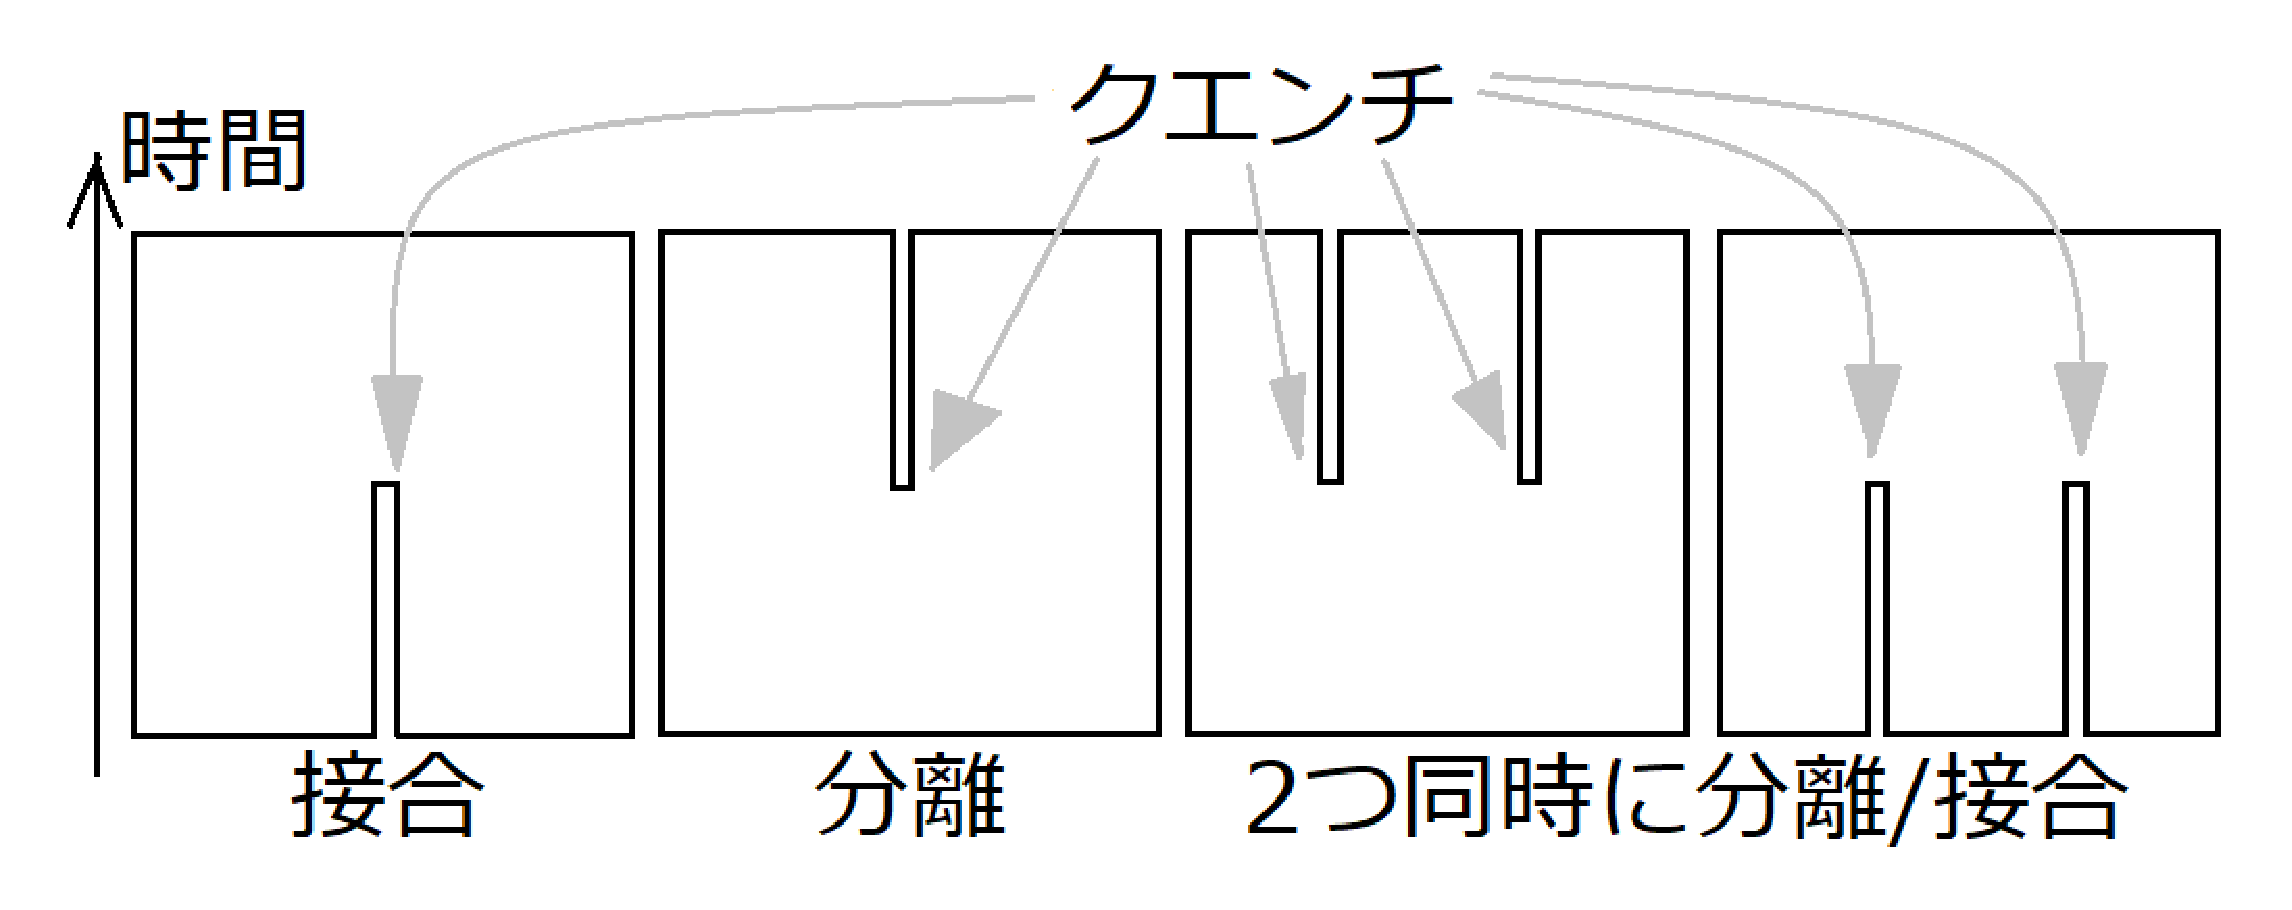
\includegraphics[width=0.7\linewidth]{quenchfig.pdf}
\end{figure}

以下に2つの論文で解析した内容の表をまとめる。
\begin{table}[H]
	\centering
	\begin{tabular}{|c||c|c|c|c|}\hline\hline
		  & 接合 & 分離 & 2重接合 & 2重分離 \\ \hline
		零質量自由Dirac場のEE & $\bigcirc$ & $\bigcirc$ & $\bigcirc$ & $\bigcirc$ \\
		重力双対を持つCFTのEE & $\bigcirc$ & $\bigcirc$ & $\bigcirc$ & $\bigcirc$ \\
		重力双対の測地線の描像 & $\bigcirc$ & $\bigcirc$ & $\bigcirc$ &  \\ \hline
	\end{tabular}
\end{table}

本論文では、分離クエンチと2重分離クエンチに焦点をあてて、その解析結果を解説する。分離クエンチは\cite{gring2012relaxation}で、二重井戸型ポテンシャルを用いて1次元冷却原子気体を2つに分離することで実験されており、実験への応用を考える上でも興味深い。また、格子系を分離クエンチしたときのEEの計算は\cite{Zamora_2014}で研究されていた。我々の解析はその連続理論版にあたる。

重力双対を持つCFTのEEの計算は、笠-高柳公式を用いて測地線の長さを計算することで行った。このとき、多くの場合で測地線はPoincare領域で覆われる領域を出て、AdS空間の大域的なトポロジーに関係することがわかった。この現象はHartman,Maldacena\cite{hartman2013time}などによって別の問題設定でも起きることが知られている。

零質量自由Dirac場はカオス性のない``可積分"な理論であるのに対して、重力双対を持つCFTは非常に強いカオス性を持つことが知られている\cite{Maldacena:2015waa}。これらのEEの振る舞いを比較することで、重力双対を持つCFTは、カオス的でない零質量自由Dirac場に比べて急速に熱平衡化が起きることが分かった。

また、2重分離クエンチでのエンタングルメントエントロピーの解析により、3次元重力理論の境界におけるboundary gravitonの自由度の存在を確認し、引力相互作用が働いていることを予想した。

\section*{本論文の構成}
本論文の構成は以下のとおりである。\ref{chap:adscftreview}章では2次元共形場理論やその具体例である自由場の理論と、3次元漸近的AdS空間の理論をして、それらのAdS$_3$/CFT$_2$対応を解説する。また本研究で用いたAdS/BCFTの処方についても解説する。\ref{chap:EEreview}章では場の理論におけるエンタングルメントの定義を述べた後、2次元共形場理論のエンタングルメントエントロピーと、AdS$_3$/CFT$_2$対応についての笠-高柳公式を解説する。

\ref{chap:singlquench}章では我々の研究\cite{Shimaji:2018czt}に基づいて、直線上の2次元共形場理論の真空を分離クエンチしたときのエンタングルメントエントロピーの時間発展を解析し、その重力双対の描像を調べる。このとき分離によって、双対なAdS$_3$空間に非常に重い障害が出来ることを見る。

\ref{chap:doublequench}章では我々の研究\cite{Caputa:2019avh}に基づいて、直線上の2次元共形場理論の真空を2重分離クエンチしたときのエンタングルメントエントロピーの時間発展を解析する。\ref{chap:singlquench}の解析から、共形場理論の2つの分離に対応してその双対なAdS$_3$空間には2つの重い障害が生じると考えられ、それらはAdS$_3$の境界に生じる重力相互作用で引き合うと考えられるが、このことをエンタングルメントエントロピーの振る舞いから解釈する。

	\chapter{AdS$_3$/CFT$_2$対応}\label{chap:adscftreview}
この章では\textbf{AdS$_3$/CFT$_2$対応}に焦点をあてて、本研究の内容を説明するために必要な事項を解説する。AdS$_{d+1}$とは$d+1$次元反 de Sitter(anti de Sitter)時空の略語で、CFT$_d$とは$d$次元共形場理論(conformal field theory)の略語であり、以降しばしばこの略語を用いる。
\newline

1995年にMaldacenaによって最初に発見された\textbf{AdS$_5$/CFT$_4$対応} \cite{Maldacena:1997re}は、「AdS$_5\times S^5$背景時空上のType IIB超弦理論」と「AdS$_5$の``境界"の$4$次元時空に存在する$\mathcal{N}=4$ 超対称SU($N$) Yang-Mills理論」の相関関数の等価性を主張する。この等価性は、Type IIB超弦理論において$N$枚のD3ブレーンを並行にならべた状況の低エネルギー極限をとることで発見された。AdS$_5$/CFT$_4$対応のほかにも、様々な理論やブレーンの配置の低エネルギー極限をとることで、「AdS$_{d+1}$背景時空上の重力理論」と「AdS$_{d+1}$の$d$次元の境界に住むゲージ理論」の相関関数が等価になる様々な具体例が構成されている\cite{Aharony:1999ti}。このとき、AdS重力に対応する場の理論には超対称性や共形対称性は必ずしも必要ではないため、このような等価性を\textbf{ゲージ重力対応(gauge gravity correspondence)}や\textbf{ホログラフィー原理(holographic principle)}などと呼ぶことも多い。

AdS$_{d+1}$/CFT$_d$対応とは「$d+1$次元AdS背景時空上の重力理論」と「$d$次元AdS空間の境界上の強結合な共形場理論(CFT)」の相関関数の等価性のことを指す予想である。この対応は現時点で数学的に証明されてはいないが、膨大な数の研究によってその等価性が検証されており、多くの研究者はこの予想が正しいと信じている。AdS$_5$/CFT$_4$対応を提唱したMaldacenaの論文\cite{Maldacena:1997re}は、素粒子物理学を中心とする論文のデータベース INSPIRE(http://inspirehep.net)において現時点で最も多い引用件数がある。また、この論文はプレプリントサーバー arXiv(https://arxiv.org)の物理のすべての分野で引用されており、現代の物理学の大きな潮流のひとつとなっている。

AdS/CFT対応を応用する手法は大きく2つに分類できる。一つは「強結合な場の理論」の相関関数を「重力理論」における測地線などの幾何学的な量に置き換える方法である。これにより一般に摂動論的な扱いが難しい強結合な理論の相関関数を、重力理論での比較的簡単な計算に置き換えることができる。そのため、AdS/CFT対応はQCD\cite{Sakai:2004cn}\cite{Kovtun:2004de}や強相関な物性系\cite{Hartnoll_2009}といった非摂動的な効果が重要になる物理系での物理量の計算にも応用されてきた。もう一つの応用法は、「(半古典)重力理論」における物理量を「強結合な場の理論」の相関関数に置き換える方法である。例えば、Bekenstein-Hawkingエントロピーは重力を半古典近似して取り扱うことで導出されたが、AdS/CFT対応によってこれを場の理論から導出することができる\cite{Strominger:1996sh}\cite{Strominger:1997eq}。
\newline

$\ref{sec:confsym},\ref{sec:2dcft},\ref{sec:2dscalar},\ref{sec:2ddirac}$節では、2次元共形場理論やその具体例である自由スカラー場や自由Dirac場を\cite{EguchiSugawara}\cite{NakaharaTop1}\cite{NakaharaTop2}\cite{NakayamaCFT}\cite{polchinski1998string1}\cite{polchinski1998string2}\cite{francesco2012conformal}を参考にして解説する。$\ref{sec:ads3}$節ではAdS/CFT対応で重要になる漸近的AdS$_3$時空を\cite{FukumaSakatani}\cite{Banados:1998gg}\cite{Donnay:2016iyk}を参考に解説する。$\ref{sec:adscft}$節ではAdS$_3$/CFT$_2$対応を\cite{TakayanagiJapan}\cite{Natsuume}\cite{Klebanov:2000me}\cite{Banerjee}を参考に解説する。最後に$\ref{sec:adsbcft}$節では、本研究で中心的な役割を果たした「境界付き漸近的AdS時空」と「境界付き空間上の共形場理論」の対応を取り扱う\textbf{AdS/BCFT}の処方を\cite{Takayanagi:2011zk}\cite{Fujita:2011fp}を参考に解説する。

\section{共形対称性}\label{sec:confsym}
ここでは\ref{sec:2dcft}節以降で2次元共形場理論を扱う準備として、共形対称性の定義を説明する。共形場理論を定義するときには「共形対称性」と「Weyl対称性」という混同しやすい概念が登場する。これらはどちらも重要な概念であるため、できるだけ誤解を排除するために若干形式的に導入する。

\subsection{古典的共形対称性}\label{subsecclassicalconfsym}
\subsub{共形変換・Weyl変換の定義}
多様体$M$からそれ自身への微分同相全体は写像の合成を積として群をなす。これを微分同相群(diffeomorphism group)といい$\text{Diff}(M)$で表す。

2つの擬Riemann多様体$(M_1,g_1),(M_2,g_2)$の間の微分同相$F\colon M_1\to M_2$が、$F^\ast g_2=e^\Omega g_1\ (\exists\Omega\in\text{C}^\infty(M_1,\R))$を満たすとき、$F$を\textbf{大域共形変換(global conformal transformation)}\footnote{数学では共形変換と呼ばれる。ここで定義した意味でも「大域共形変換」は「共形変換」になっているので、「任意の共形変換」と言った場合には大域共形変換も含まれることになる。}という。大域共形変換$F\colon M_1\to M_2$が存在するとき、$(M_1,g_1)$と$(M_2,g_2)$は\textbf{共形同値(conformally equivalent)}であるといい、平坦な多様体に共形同値な擬Riemann多様体は\textbf{共形平坦(conformally flat)}であるという。また、2つの擬Riemann多様体$(M_1,g_1),(M_2,g_2)$の部分空間$U_1\of M_1,U_2\of M_2$の間の大域共形変換$F\colon U_1\to U_2$を局所共形変換、あるいは誤解のない限りたんに\textbf{共形変換(conformal transformation)}という。

擬Riemann多様体$(M,g)$からそれ自身への大域共形変換全体は写像の合成を積として群をなす。これを大域共形変換群\footnote{普通は共形変換群という。ここではあえて大域をつけている。}といい$\text{Conf}(M,g)$と書く。明らかに$\text{Conf}(M,g)$は$\text{Diff}(M)$の部分群になっている。また大域共形変換群$\text{Conf}(M,g)$はその定義から、等長変換群$\text{Isom}(M,g)$を部分群に含む。

\begin{ex}
任意の2次元Riemann多様体は局所的に共形平坦\footnotemark であり、向き付け可能であれば複素構造が自動的に入ってRiemann面(Riemann surface)になる。共形変換の定義より、Riemann面上の局所共形変換とは局所的な双正則変換(biholomorphic transformation)のことであり、大域共形変換群とは正則自己同型群(automorphism group)のことである。
\end{ex}
\footnotetext{{2次元Riemann多様体に局所的な共形平坦座標である等温座標(isothermal coordinate)がとれることから従う。}}

多様体$M$に許容される$(p,q)$型の符号を持った計量$g$の全体を$\text{Met}(M,(p,q))$、あるいはたんに$\text{Met}(M)$と書くことにする。例えば、$M$上のRiemann計量全体は$\text{Met}(M,(d,0))$と書けて、$M$上のLorentz計量全体は$\text{Met}(M,(d-1,1))$と書ける。

いま、計量$g$と$e^\Omega g\ (\Omega\in\text{C}^\infty(M,\R))$の符号は変わらないので、$M$上でつねに正の値をとる関数$e^\Omega$を掛けてスケール変換する写像$g\mapsto e^\Omega g$は$\text{Met}(M,(p,q))$からそれ自身への写像となる。このスケール変換$e^\Omega\colon \text{Met}(M,(p,q))\to \text{Met}(M,(p,q))$を\textbf{Weyl変換(Weyl transformation)}\footnote{この変換を共形変換と呼ぶ流儀もあるので、注意しておく。}という。Weyl変換も写像の合成を積として群をなし、これを$\text{Weyl}(M,(p,q))$、あるいはたんに$\text{Weyl}(M)$と書く。共形変換(群)は計量を固定しなければ定義できなかったが、微分同相変換やWeyl変換は計量を固定せずに定義できることに注意する。

2つの計量$g,g'$がWeyl変換で移りあうなら$\text{Conf}(M,g)=\text{Conf}(M,g')$となるから、大域共形変換群はWeyl変換の同値類にしか依らない。そこで$\text{Conf}(M,g)$のことを、$\text{Conf}(M,[g])$と書くことも多い。ただし$[g]\in\text{Met}(M)/\text{Weyl}(M)$は$g$のWeyl同値類である。

\subsub{共形Killing方程式}
局所共形変換を生成する、$U\of M$上で局所的に定義されたベクトル場$v$を求めるためには、\textbf{共形Killing方程式}$\mathcal{L}_v g=fg\ (\exists f\in\text{C}^\infty(U,\R)))$を解けばいい。

共形Killing方程式を成分表示すると、$\nabla_\mu v_\nu(x)+\nabla_\nu v_\nu(x)=f(x)g_{\mu\nu}$であり、両辺のトレースをとれば、
\begin{align}\label{confkilling}
\nabla_\mu v_\nu+\nabla_\nu v_\mu=\frac{2}{d}g_{\mu\nu} \nabla_\rho v^\rho 
\end{align}
と$v$のみで書ける。

\begin{ex}
とくに平坦空間の場合、$\ g_{\mu\nu}=\eta_{\mu\nu},\nabla_\mu=\del_\mu$であり、共形Killing方程式から
\begin{align}
2\del^2 v_\nu=(2-d)\del_\nu f,\quad (2-d)\del_\nu\del_\rho f=\eta_{\nu\rho} \del^2 f,\quad (d-1)\del^2 f=0
\end{align}
という式を得る。したがって$d\geq 3$の平坦空間$\R^{(p,q)}$\footnotemark なら$\del_\mu\del_\nu f=0$となり、$f(x)=A+B_\mu x^\mu,\ (A,B_\mu\text{は定数})$の形のみ許され、$v$は$x^\mu$の2次式の形に制限される。これに注意して共形Killing方程式を解けば、$v$は次の4種類のベクトル場の線形結合として表されることが分かる。
\begin{align}
&\text{並進}&&P_\mu\coloneqq \del_\mu&&\\
&\text{回転(Lorentz変換)}&&M_{\mu\nu}\coloneqq x_\nu\del_\mu-x_\mu\del_\nu&&\\
&\text{スケール変換}&&D\coloneqq x^\mu\del_\mu&&\\
&\text{特殊共形変換}&&K_\mu\coloneqq 2x_\mu x^\nu\del_\nu-x^2\del_\mu&&
\end{align}

これらの生成子は次の交換関係を満たし、$\so(p+1,q+1)$の生成子となっている。また、$\text{Isom}(M,g)\of \text{Conf}(M,g)$よりポアンカレ群の生成子$P_\mu, M_{\mu\nu}$が含まれていることに注意する。
\begin{align}
[D,P_\mu]&=P_\mu\\
[K_\rho,D]&=K_\rho\\
[K_\rho,P_\mu]&=2(\eta_{\rho\mu}D-M_{\rho\mu})\\
[K_\rho,M_{\mu\nu}]&=\eta_{\rho\mu}K_\nu-\eta_{\rho\nu}K_\mu\\
[P_\rho,M_{\mu\nu}]&=\eta_{\rho\mu}P_\nu-\eta_{\rho\nu}P_\mu\\
[M_{\mu\nu},M_{\rho\sigma}]&=\eta_{\mu\sigma}M_{\nu\rho}+\eta_{\nu\rho}M_{\mu\sigma}-\eta_{\mu\rho}M_{\nu\sigma}-\eta_{\nu\sigma}M_{\mu\rho}
\end{align}
$P_{\mu},M_{\mu\nu},D,K_{\mu}$に対応する有限変換は
\begin{align}
&\text{並進}&&x^\mu \mapsto x^\mu+a^\mu&&\\
&\text{回転(Lorentz変換)}&&x^\mu\mapsto M^\mu_\nu x^\nu\  (M\in SO_+(p,q))&&\\
&\text{スケール変換}&&x^\mu \mapsto e^\alpha x^\mu&&\\
&\text{特殊共形変換}&& x^\mu\mapsto \frac{x^\mu-c^\mu x^2}{1-2c_\nu x^\nu+c^2x^2} &&
\end{align}
で与えられる。共形対称性は特殊共形変換に対する不変性も含む言葉なので、スケール不変性を持つ理論は共形場理論になるとは限らないことに注意しておく。
\end{ex}
\footnotetext{$\R^{(p,q)}$とは、平坦計量$\eta=\text{diag}(\overbrace{+1,\cdots,+1}^{p},\overbrace{-1,\cdots,-1}^{q})$を持った$p+q$次元平面のこと。}

\begin{ex}
Riemann面に共形平坦な局所座標$(x,\tau)$をとり、$g_{\mu\nu}(x,\tau)=e^{2\Omega(x,\tau)}\delta_{\mu\nu}$とする。このとき共形Killing方程式(\ref{confkilling})は$\Omega$に依らず、Cauchy-Riemann方程式
\begin{align}
\del_x v^x=\del_\tau v^\tau,\ \del_x v^\tau= -\del_\tau v^x
\end{align}
になる。共形平坦座標$(x,\tau)$に対して複素座標と複素微分
\begin{align}
&z\coloneqq x+i\tau, &&\overline{z}\coloneqq x-i\tau&&\\
&\del\coloneqq \del_z=\frac{1}{2}(\del_x-i\del_\tau), &&\overline{\del}\coloneqq \del_{\overline{z}}=\frac{1}{2}(\del_x+i\del_\tau)&&
\end{align}
を導入すると、共形Killing方程式(\ref{confkilling})は
\begin{align}
\del_z v^{\overline{z}}=0,\  \del_{\overline{z}} v^z=0
\end{align}
に等しい。したがってRiemann面上の局所共形変換を生成するベクトル場は、局所的に定義された正則・反正則ベクトル場に他ならない。

境界のない種数$g$のコンパクトRiemann面$\Sigma_g$上の大域的な共形Killingベクトル場(=正則ベクトル場)の自由度と、共形Killing群(=正則自己同型群の単位元に連結な成分)は
\begin{table}[H]
	\centering
	\begin{tabular}{|c|c|c|}\hline
		g & $\dim_\R$\{正則ベクトル場全体\} & 共形Killing群 \\ \hline
		$0$ & 6 & $PSL(2,\C)$ \\\hline
		$1$ & 2 & $U(1)\times U(1)$\\\hline
		$2$以上 & 0 & $\{1\}$\\ \hline
	\end{tabular}
\end{table}
となる。とくに$\Sigma_0=S^2$の正則自己同型群は
\begin{align}
Aut(S^2)=PSL(2,\C)=SO_+(3,1)=\left\{ \frac{az+b}{cz+d} \mid a,b,c,d\in \C,\ ad-bc\neq 0 \right\}
\end{align}
であり、$d\geq 3$の平坦空間$\R^{(p,q)}$の場合の結果に一致する。また、このLie群の6つの生成子として並進$P_\mu$、回転$M$、スケール変換$D$、特殊共形変換$K_\mu$ ($\mu=1,2$)がとれる。

$\Sigma_1=T^2$の共形Killing群$U(1)\times U(1)$は小円・大円の接線方向への並進変換(図\ref{fig:torusckv})に対応している。また、$\Sigma_{g\geq 2}$の正則自己同型群は有限群になる。

\begin{figure}[h]
	\centering
	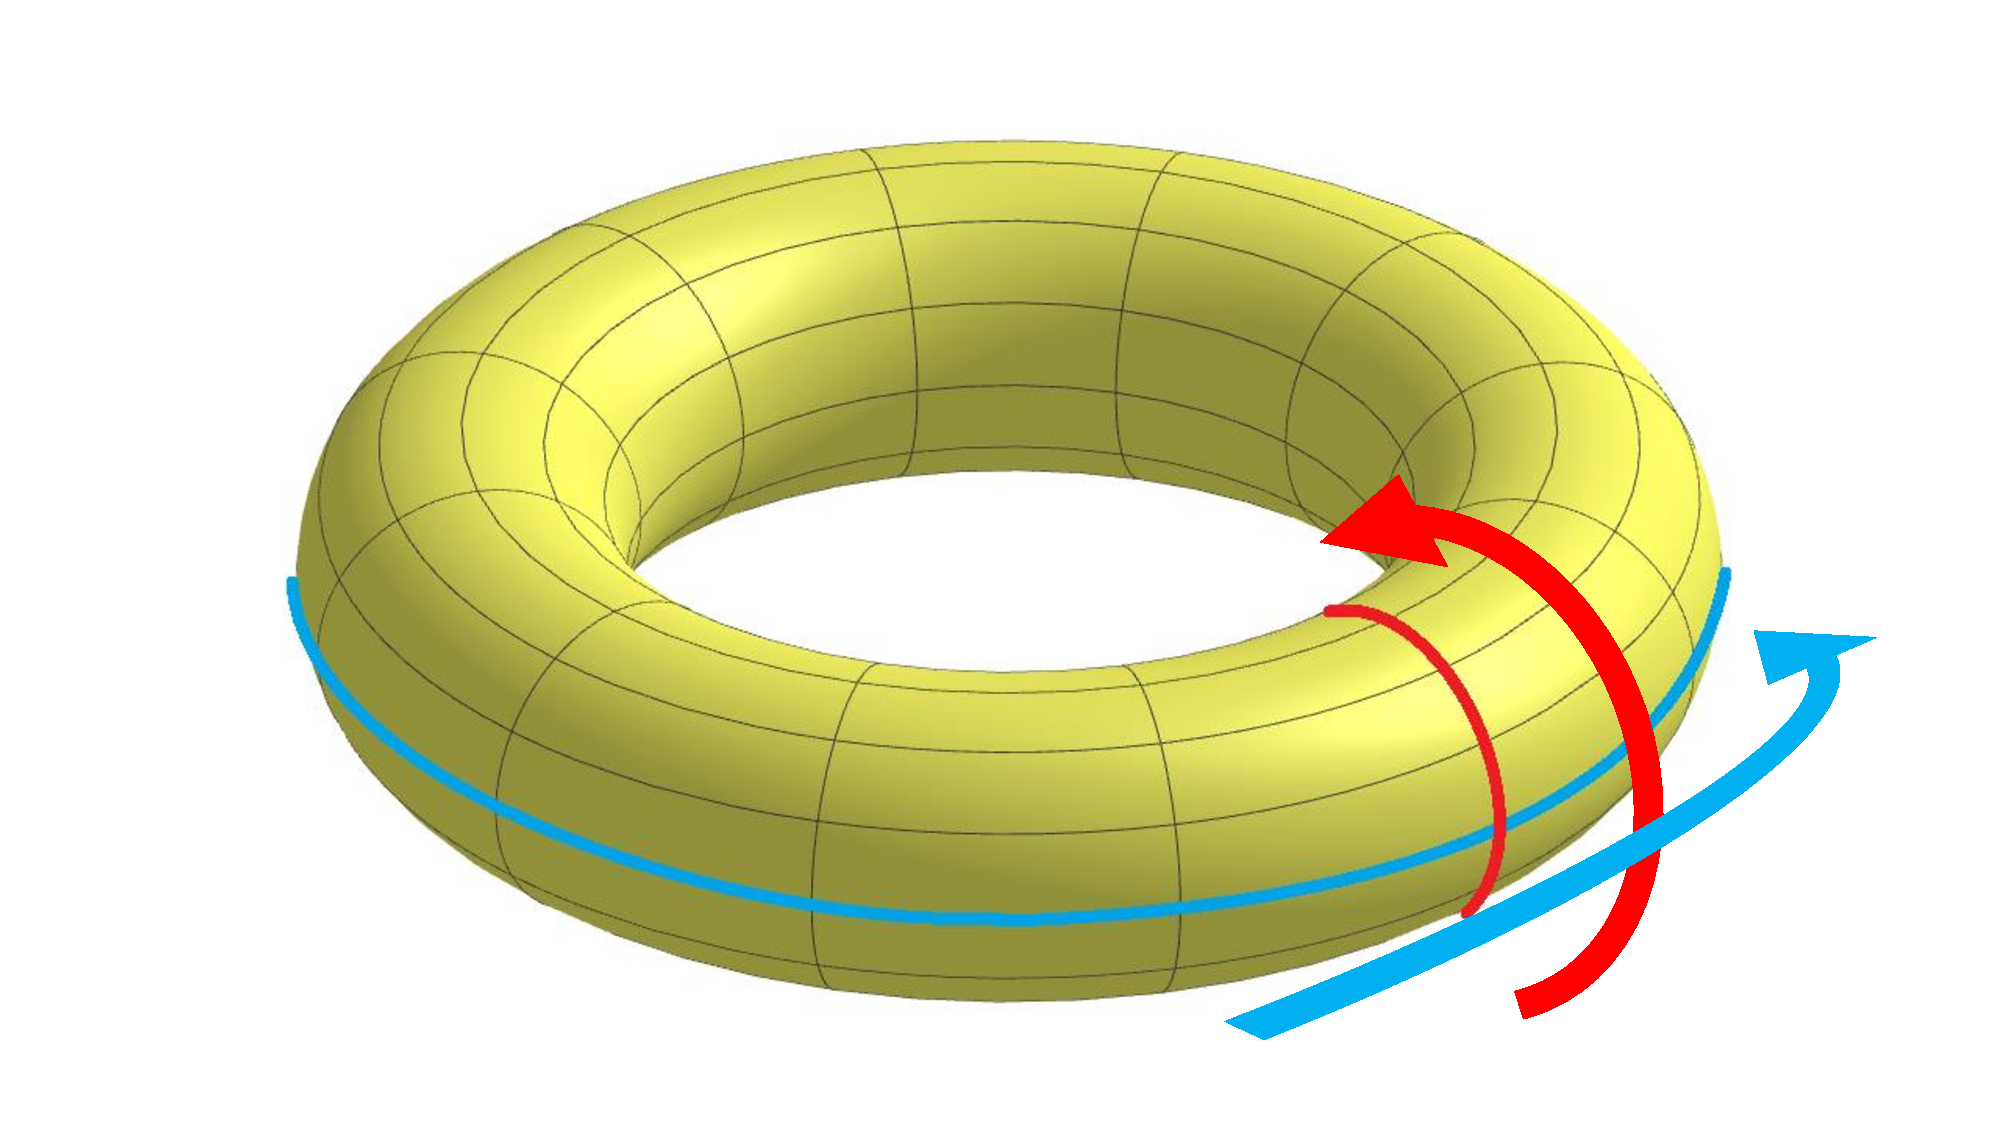
\includegraphics[width=0.7\linewidth]{torusCKV.pdf}
	\caption{トーラスの小円(赤線)と大円(青線)の接線方向が共形Killingベクトルになる。}
	\label{fig:torusckv}
\end{figure}


一般に$2$つのRiemann面が微分同相であっても共形同値になるとは限らない。そこで$1$つRiemann面$M$を与えたときに、$M$に微分同相な多様体全体の集合を共形同値なもので分類することを考えてみる。つまり
\begin{align}
\{ N\mid N\text{は}M\text{に微分同相} \}/\text{共形同値}
\end{align}
という分類を考えてみる。

単連結Riemann面についての分類は、K\"{o}beの一意化定理(uniformization theorem)として知られていて、任意の単連結Riemann面は平面$\C$、円板$D^2$、球面$S^2$のいずれかに共形同値であることが知られている。

境界のない、計量$\gamma$をもった種数$g$のコンパクトRiemann面$(\Sigma_g,\gamma)$についての分類集合
\begin{align}
\text{Mod}_g=\{ N\mid N\text{は}\Sigma_g\text{に微分同相} \}/\text{共形同値}
\end{align}
は$(\Sigma_g,\gamma)$のモジュライ空間(moduli space)と呼ばれ、
\begin{align}
\dim_\C \text{Mod}_g=\left\{ \begin{array}{cc}   
0 &(g=0)\\
1 &(g=1)\\
3g-3 &(g=2)
\end{array}\right.
\end{align}
であることが知られている。

たとえば$g=1$のときを考えてみる。$z\sim z+2\pi \sim z+2\pi\tau\ (\IM\tau>0)$と同一視の入った平坦トーラス $T_\tau^2\  (ds^2=dzd\overline{z})$を考え(図\ref{fig:flattorus})、モジュライパラメータを
\begin{align}
\tau' = \frac{a\tau+b}{c\tau+d}\quad (a,b,c,d\in \Z,\  ad-bc=1)
\end{align}
と$PSL(2,\Z)$変換することを考える。$PSL(2,\Z)$群は$2$つの元
\begin{align}
\tau'&= -\frac{1}{\tau}\\
\tau'&= \tau+1
\end{align}
で生成され、これらの変換は\textbf{モジュラー変換(modular transformation)}と呼ばれる。
\begin{figure}[h]
	\centering
	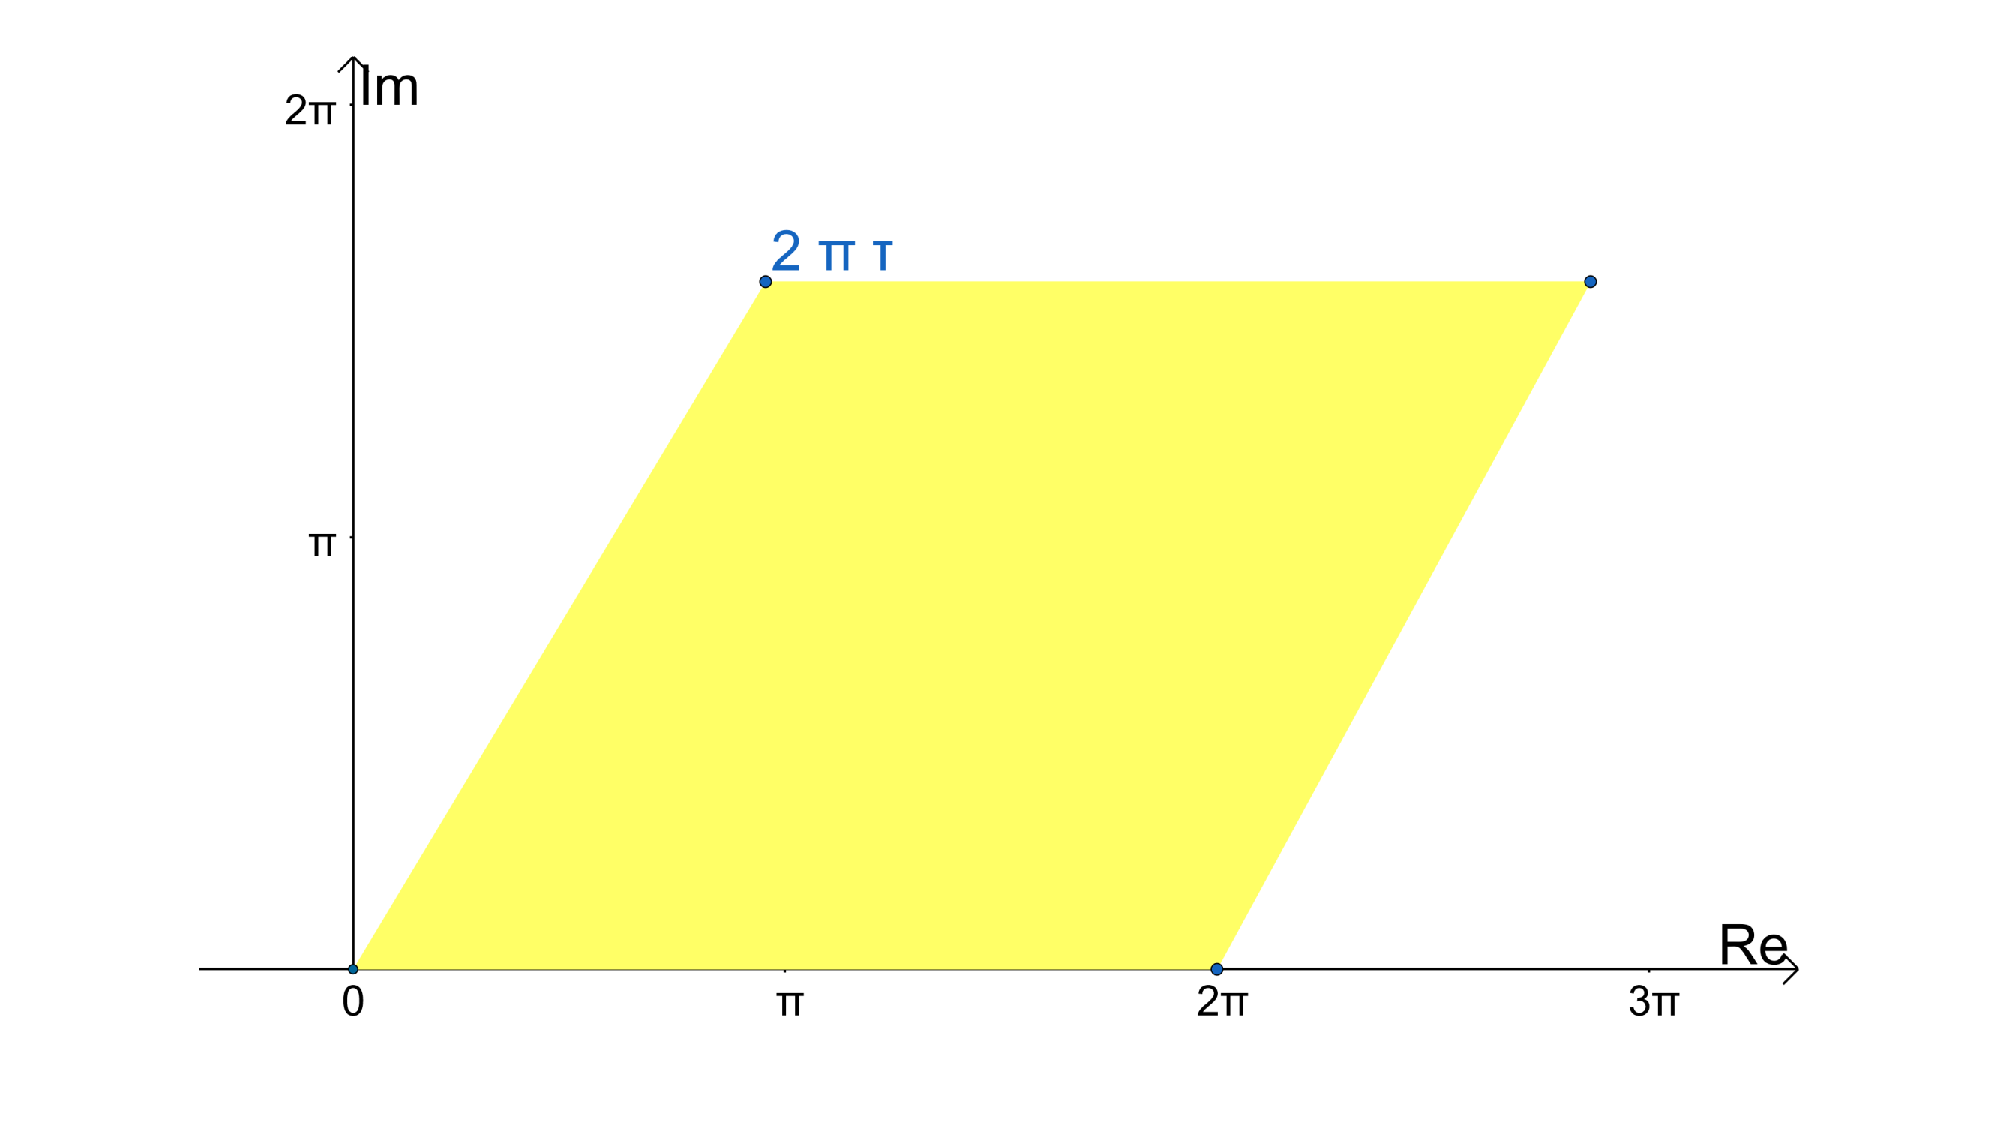
\includegraphics[width=0.7\linewidth]{flattorus.pdf}
	\caption{平坦トーラスを表す平行四辺形。2つの対辺をそれぞれ同一視することで平坦なトーラスを4次元空間に実現することができる。}
	\label{fig:flattorus}
\end{figure}

上のモジュラー変換に対して平坦トーラス$T_{\tau'}^2$は$T_{\tau}^2$とスケール変換で移りあうから、これらは共形同値である。したがって$\tau\ (\IM\tau>0)$を同一視のパラメータにもつ平坦トーラス$T_{\tau}^2$は、パラメータを$PSL(2,\Z)$変換しても共形同値であることが分かる。

トーラスのモジュライ空間$\text{Mod}_1$は$\UHP/PSL(2,\Z)$になり、たしかに$\dim_\C \text{Mod}_1=1$となっている。同一視のパラメータ$\tau$はモジュライ空間の座標を与えるので、\textbf{モジュライパラメータ(moduli parameter)}と呼ばれる。
\end{ex}

\subsub{作用の古典的共形対称性}
$d$次元(擬)Riemann多様体$(M,g)$を時空にもつ場$X$の理論を考える。計量$g$を力学変数として扱う場合、その古典作用を$S[X,g]$で表す。計量$g$を力学変数として扱わず、背景時空として外場と見なす場合、その古典作用を$S[X]_{(M,g)}$で表す\footnote{定義から当然、$S[X,g]=S[X]_{(M,g)}$なのだが、$g$が力学変数になっているか否かで敢えてノーテーションを分けた。例えば4次元Minkowski空間上のスカラー場のラグランジアン$\frac{1}{2}\eta^{\mu\nu}\del_\mu \phi \del_\nu \phi+\frac{1}{2}m\phi^2$を考えるときには、計量は$\eta$で固定されていて、これは右辺のノーテーションになっている。しかし一般相対論ではEinstein-Hilbert作用とともに、$g$に結合したスカラー場のラグランジアン$\frac{1}{2}g^{\mu\nu}\del_\mu \phi \del_\nu \phi+\frac{1}{2}m\phi^2$が使われ、これは左辺のノーテーションになっている。}。
\begin{oframed}
作用$S[X,g]$の(古典的)\textbf{微分同相不変性}と(古典的)\textbf{Weyl不変性}をそれぞれ次で定義する。
\begin{align}
&S[X,g]\text{が微分同相不変}&&\iff \forall F\in\text{Diff}(M),&& S[F^\ast X,F^\ast g]=S[X,g]&&\\
&S[X,g]\text{がWeyl不変}&&\iff \forall e^\Omega \in\text{Weyl(M)},&& S[X,e^\Omega g]=S[X,g]&&
\end{align}
また、時空を固定した上で、作用$S[X]_{(M,g)}$の(古典的)\textbf{共形不変性}を次で定義する。
\begin{align}
&S[X]_{(M,g)}\text{が共形不変}&&\iff \forall F;\text{ 局所共形変換},&& S[F^\ast X]_{(M,g)}=S[X]_{(M,g)}&&
\end{align}
これが古典的な共形場理論の定義である。
\end{oframed}

微分同相不変な$S[X,g]$がWeyl不変ならば
\begin{align}
S[F^\ast X]_{(M,g)}=S[F^\ast X,g]=S[X,(F^{-1})^\ast g]=S[X,e^{-\Omega}g]=S[X,g]=S[X]_{(M,g)}
\end{align}
より、$S[X]_{(M,g)}$は共形不変となる。しかし逆は成り立たない。

背景時空を固定した作用$S[X]_{(M,g)}$に対して、場$X$の\textbf{エネルギー運動量テンソル}$T^X_{\mu\nu}(x)$を求めるには、$g$を力学変数と思って$S[X]_{(M,g)}=S[X,g]$として、
\begin{align}\label{defEMtensor}
T^X_{\mu\nu}\coloneqq -\frac{4\pi}{\sqrt{|\det g|}}\frac{\delta S[X,g]}{\delta g^{\mu\nu}}
\end{align}
と定義すればいい。

関数$\Omega\in\text{C}^\infty(M,\R)$による1パラメータWeyl変換群$e^{s\Omega}\ (s\in\R)$を考え、これにより生成される無限小共形変換$\delta_\Omega g= \Omega g$を考えると、共形Killing方程式(\ref{confkilling})から、
\begin{align}
\delta_\Omega S[X,g]&=\frac{1}{2}\int d^d x \sqrt{|\det g|}(T^X)^{\mu\nu}\delta_\Omega g_{\mu\nu}\notag\\
&=\frac{1}{2}\int d^d x \sqrt{|\det g|}\Omega (T^X)^{\mu}_{\ \mu}
\end{align}
となる。よって$S[X]_{(M,g)}$を拡張した作用$S[X,g]$のWeyl不変性は$\forall x\in M,\ (T^X)^{\mu}_{\ \mu}(x)=0$となることに同値である。

したがって$(T^X)^{\mu}_{\ \mu}=0$となる作用$S[X]_{(M,g)}$は(古典的に)共形不変になることが分かった。しかし逆は成り立たないことに注意しておく。
\begin{ex}
$d$次元平坦空間上の質量$m$の自由スカラー場$\mathcal{L}=\frac{1}{2}((\del X)^2-m^2 X^2)$のエネルギー運動量テンソルは、
\begin{align}
\frac{1}{2\pi}T_{\mu\nu}=\del_\mu X \del_\nu X-\frac{1}{2}\eta_{\mu\nu}((\del X)^2-m^2 X^2)
\end{align}
で与えられ、そのトレースは
\begin{align}
\frac{1}{2\pi}T^\mu_{\ \mu}=\left(1-\frac{d}{2}\right)(\del X)^2+\frac{1}{2}m^2 X^2
\end{align}
となる。したがって2次元平坦空間上の零質量$(m=0)$自由スカラー場は古典的に共形不変な理論になる。
\end{ex}

\begin{ex}
$d$次元平坦空間上の$U(1)$Yang-Millsゲージ場$\mathcal{L}=-\frac{1}{4}F^2$のエネルギー運動量テンソルは
\begin{align}
\frac{1}{2\pi}T_{\mu\nu}=-\eta^{\rho\sigma}F_{\mu\rho}F_{\sigma\mu}+\frac{1}{4}\eta_{\mu\nu}F^2
\end{align}
で与えられ、そのトレースは
\begin{align}
\frac{1}{2\pi}T^{\mu}_{\ \mu}=\left(\frac{d}{4}-1\right)F^2
\end{align}
となる。したがって4次元平坦空間上の電磁場は古典的に共形不変な理論になる。
\end{ex}

\subsection{Weylアノマリー}
\ref{subsecclassicalconfsym}節では古典的なWeyl対称性が、エネルギー運動量テンソルのトレースが$0$になることと同値であることを見た。しかし量子論を考えると、計量$g$の経路積分をするときに経路積分測度が対称性を破って期待値$\la T^{\mu}_{\ \mu}\ra$が$0$にならないことがある。このときWeyl対称性は量子論的に破れており、\textbf{Weylアノマリー(Weyl anomaly)}あるいはトレースアノマリーがあるという\footnote{微分同相不変性や共形不変性のアノマリーを考えることもできるが、それらのアノマリーはふつうWeylアノマリーと関係して生じており、微分同相不変/共形不変な正則化を用いることでアノマリーをすべてWeylアノマリーに押し付けることができる。したがってここでは微分同相不変性や共形不変性はアノマリーがないと仮定する。}。

$\la T^\mu_\mu\ra$は質量次元$d$であり大域的共形変換で値が変わらない。一般に$\la T^\mu_\mu\ra$はEuler類$e(x)
$\footnote{接束$TM$の構造群を$SO(2n)$に簡約したとき、曲率$R$は$so(2n)$値$2$形式となる。Euler類はこの行列$R$に対して、$e(x)=\text{Pf}(R(x))/(2\pi)^n$で定義される、主$SO(2n)$束の特性類である。ただし$\text{Pf}$はパフィアンを表していて、$\text{Pf}(R)^2=\det R$を満たす。}
と、Weylテンソル$C_{\mu\nu\rho\sigma}(x)
$\footnote{$d$次元擬Riemann多様体におけるWeylテンソルは
\begin{align}
R_{\mu\nu\rho\sigma}=\frac{1}{d-2}\left(g_{\mu\rho}R_{\sigma\nu}-g_{\mu\sigma}R_{\rho\nu}+g_{\nu\sigma}R_{\rho\mu}-g_{\nu\rho}R_{\sigma\mu}-\frac{1}{d-1}R(g_{\mu\rho}g_{\sigma\nu}-g_{\mu\sigma}g_{\rho\nu})\right)+C_{\mu\nu\rho\sigma}
\end{align}
で定義される。Weylテンソルは$d(d+1)(d+2)(d-3)/12$個の自由度を持ち、$d\leq 3$次元では消える。またWeylテンソルは計量のWeyl変換に対して不変である。}
を縮約して得られる質量次元$d$のスカラー量たち$I_i(x)$の線形和になることが知られている\cite{Deser:1993yx}。とくに奇数次元ではEuler類は消え、Weylテンソルを縮約して得られる質量次元が奇数のスカラー量も無いので、Weylアノマリーは出ない。

$2$次元ではEuler類$e$はリッチスカラー$R$であり、Weylテンソルも消えるので、$2$次元多様体でのWeylアノマリーは無次元の定数$c$とリッチスカラー$R$と分配関数$Z$を用いて
\begin{oframed}
\begin{align}\label{confanomaly2d}
\la T^{\mu}_{\ \mu}(x) \ra=-\frac{c}{12}R(x)
\end{align}
\end{oframed}
の形になる。

\section{2次元共形場理論(CFT$_2$)}\label{sec:2dcft}
ここでは共形対称性をもった2次元の場の量子論の一般論を説明する。共形場理論は$1+1$次元と$1+d\ (d\leq2)$次元で無限小の対称性の性質が大きく異なる。そのため$1+d\ (d\leq2)$次元の共形場理論はしばしば高次元共形場理論と呼ばれ、$1+1$次元共形場理論と区別することが多い。ここでは$1+1=2$次元共形場理論に焦点をあてて、その量子論的な性質を論じる。

2次元共形場理論はBelavin,Polyakov,Zamolodchikov \cite{Polyakov:1970xd}\cite{Belavin:1984vu}によって導入され、スケール不変性を持つ理論や、無限個の対称性を持つ理論として、物理や数理物理のさまざまな分野に関連して発展してきた。とくにVirasoro対称性やCardy公式といった、2次元共形場理論特有の性質はAdS$_3$/CFT$_2$対応においても重要な役割を果たす。

\subsection{プライマリー場}
ローレンツ不変な場の理論ではローレンツ共変な場が基本的な役割を果たすが、共形場理論においてこれに相当する場はプライマリー場と呼ばれる。
\begin{oframed}
共形変換$z\mapsto f(z),\overline{z}\mapsto \overline{f}(\overline{z})$のもとでの場$\Phi$の変換$\Phi\mapsto f^\ast \Phi$が実数$h,\overline{h}$に対して次を満たすとき、$\Phi$を\textbf{共形ウェイト(weight)}$(h,\overline{h})$をもつ\textbf{プライマリー場(primary field)}という。
\begin{align}
(f^\ast\Phi)(z,\overline{z})=\Phi(f(z),\overline{f}(\overline{z}))\left(\frac{df(z)}{dz}\right)^h\left(\frac{d\overline{f}(\overline{z})}{d\overline{z}}\right)^{\overline{h}}
\end{align}
\end{oframed}

\begin{ex}
$S^2$上の大域共形変換である並進変換$f_T(z)=z+a$、スケール変換$f_D(z)=e^\alpha z$、回転$f_R(z)=e^{i\theta}z$、特殊共形変換$f_S(z)=z/(1-\overline{c}z)$に対してプライマリー場は
\begin{align}
(f_T^\ast\Phi)(z,\overline{z})&=\Phi(z+a,\overline{z}+\overline{a})\label{primarytranslation}\\
(f_D^\ast\Phi)(z,\overline{z})&=\Phi(e^\alpha z,e^\alpha\overline{z})e^{\alpha (h+\overline{h})}\label{primarydilation}\\
(f_R^\ast\Phi)(z,\overline{z})&=\Phi(e^{i\theta}z,e^{-i\theta}\overline{z})e^{i\theta (h-\overline{h})}\label{primaryrotation}\\
(f_S^\ast\Phi)(z,\overline{z})&=\Phi\left(\frac{z}{1-\overline{c}z},\frac{\overline{z}}{1-c\overline{z}}\right)\frac{1}{(1-\overline{c}z)^h(1-c\overline{z})^{\overline{h}}}
\end{align}
と変換する。したがって$h+\overline{h}$は$\Phi$のスケーリング次元を与え、$h-\overline{h}$は$\Phi$のスピンを与えることが分かる。
\end{ex}

\subsection{共形Ward恒等式}
次に、共形対称性を量子論的に扱うさいに重要になる共形Ward恒等式を紹介する。

コンパクトRiemann面$(\Sigma,g)$を背景にもつ理論$S[X]_{(M,g)}=S[X,g]$が古典的にも量子的にも微分同相不変であるときを考える。このとき、正則・反正則とは限らないベクトル場$v$によって生成される無限小微分同相$\delta_v$での、一般の場$\Phi_i$の相関関数の変換性を考えることで、微分同相不変性に対するWard恒等式を得る。
\begin{align}
\frac{1}{2\pi}\int_\Sigma d^2 x \sqrt{g} \nabla_\mu v_\nu(x) \la T^{\mu\nu}(x)\prod_{i=1}^N \Phi_i(x_i) \ra+ \sum_{i=1}^{N} \la \Phi_1(x_1)\cdots\delta_v \Phi_i(x_i)\cdots \Phi_N(x_N) \ra=0
\end{align}

さらに、$S[X,g]$はWeyl対称性を持ち、Weylアノマリーも無いとする。このとき$T^{\mu}_{\ \mu}=0$となるが、この条件は複素座標では$T_{z\overline{z}}=0$と書ける。したがって複素座標での$T_{\mu\nu}$は$T_{zz},T_{\overline{z}\overline{z}}$成分しか持たない。局所的な正則ベクトル場$v$によって生成される無限小共形変換による変分はエネルギー運動量テンソルの$T_{zz}$成分のみを出して、上のWard恒等式は
\begin{align}\label{confward}
\frac{1}{\pi}\int_\Sigma d^2 z \overline{\del}v(z)\la T_{zz}(z,\overline{z})\prod_{i=1}^N \Phi_i(z_i,\overline{z}_i) \ra+ \sum_{i=1}^{N} \la \Phi_1(z_1,\overline{z}_1)\cdots\delta_v \Phi_i(z_i,\overline{z}_i)\cdots \Phi_N(z_N,\overline{z}_N) \ra=0
\end{align}
となる。これを\textbf{共形Ward恒等式}という。反正則ベクトル場で変分すれば、$T_{\overline{z}\overline{z}}$に対する共形Ward恒等式を得る。

共形Ward恒等式は、共形対称性に対する量子論的な保存則を表しており、共形場理論を考える上で重要な役割を果たす。以下では共形Ward恒等式から導出される、共形場理論特有の性質を見ていく。

\subsub{エネルギー運動量テンソルの正則性}
とくに局所的な正則ベクトル場$v$として、演算子$\Phi_i$の挿入点$(z_i,\overline{z}_i)$の近傍で$0$になるものをとれば、$\delta_v \Phi_i=0$であり、(\ref{confward})を部分積分して
\begin{align}
\la \overline{\del} T_{zz}(z,\overline{z})\prod_{i=1}^N \Phi_i(z_i,\overline{z}_i) \ra=0
\end{align}
を得る。したがって$\Phi_i$の挿入点近傍以外では$T_{zz}$は正則であることが分かる。同様に、$T_{\overline{z}\overline{z}}$は場の挿入点近傍以外で反正則である。そこで以後$T(z)=T_{zz}(z),\overline{T}(\overline{z})=T_{\overline{z}\overline{z}}(\overline{z})$と書く。

$T_{zz}$の正則性は、古典的にはエネルギー保存則に他ならない。古典的な運動方程式のもとでエネルギー運動量保存$\del^\mu T_{\mu\nu}=0$が成り立ち、これを複素座標で書けば、
\begin{align}
\overline{\del} T_{zz}=0,\quad \del T_{\overline{z}\overline{z}}=0
\end{align}
であり、$T_{zz},T_{\overline{z}\overline{z}}$は正則・反正則である。
\subsub{大域的共形変換}
大域共形変換が共形Killingベクトル場(=大域的に定義された正則ベクトル場)によって生成されている場合、共形Ward恒等式(\ref{confward})の第1項は正則性から消えて、
\begin{align}
\sum_{i=1}^{N} \la \Phi_1(z_1,\overline{z}_1)\cdots\delta_v \Phi_i(z_i,\overline{z}_i)\cdots \Phi_N(z_N,\overline{z}_N) \ra=0
\end{align}
となる。つまり相関関数$\la \Phi_1(z_1,\overline{z}_1)\cdots\Phi_N(z_N,\overline{z}_N) \ra$は正則ベクトル場によって生成される大域共形変換で不変になる。したがって$S^2$上の相関関数は$PSL(2,\C)$不変になり、$T^2$上の相関関数は$U(1)\times U(1)$不変になる。

\begin{ex}
特に$S^2$上の相関関数の$PSL(2,\C)$不変性に注目してみる。$\dim_\C PSL(2,\C)=3$なので$S^2$上のプライマリー場の$N$点関数($N\leq 3$)は、$PSL(2,\C)$不変性から定数倍を除いて完全に決定される。$N\geq 4$については$PSL(2,\C)$不変な量である複比(cross ratio)
\begin{align}
x_{ij}^{kl}=\frac{(z_i-z_j)(z_k-z_l)}{(z_i-z_k)(z_j-z_l)}
\end{align}
への依存性が、相関関数の$PSL(2,\C)$不変性のみからは決定できず、それぞれの共形場理論によって異なる。

したがって共形ウェイト$(h_i,\overline{h}_i)$をもつプライマリー場$\Phi_i$の$S^2$上の$2,3,4$点関数は次のようになる。
\begin{oframed}
\begin{description}
	\item[$2$点関数] 
	\begin{align}
	\la \Phi_1(z_1,\overline{z}_1)\Phi_2(z_2,\overline{z}_2) \ra = \left\{
	\begin{array}{ll}
	\dfrac{(\text{const})}{(z_1-z_2)^{2h_1}(\overline{z}_1-\overline{z}_2)^{2\overline{h}_1}}\quad &(h_1=h_2,\overline{h}_1=\overline{h}_2)\bigskip\\
	0 &(otherwise)
	\end{array}
	\right.
	\end{align}
	
	\item[$3$点関数] 
	\begin{align}
	&\la \Phi_1(z_1,\overline{z}_1)\Phi_2(z_2,\overline{z}_2)\Phi_3(z_3,\overline{z}_3) \ra \notag\\
	&= (\text{const})\times \frac{1}{(z_1-z_2)^{h_1+h_2-h_3}(z_2-z_3)^{h_2+h_3-h_1}(z_3-z_1)^{h_3+h_1-h_2}}\notag\\
	&\qquad\qquad \times \frac{1}{(\overline{z}_1-\overline{z}_2)^{\overline{h}_1+\overline{h}_2-\overline{h}_3}(\overline{z}_2-\overline{z}_3)^{\overline{h}_2+\overline{h}_3-\overline{h}_1}(\overline{z}_3-\overline{z}_1)^{\overline{h}_3+\overline{h}_1-\overline{h}_2}}
	\end{align}
	
	\item[$4$点関数] 
	\begin{align}
	&\la \Phi_1(z_1,\overline{z}_1)\Phi_2(z_2,\overline{z}_2)\Phi_3(z_3,\overline{z}_3)\Phi_4(z_4,\overline{z}_4) \ra \notag\\
	&= \prod_{i<j}(z_i-z_j)^{-h_i-h_j+\frac{1}{3}\sum_{k=1}^{4}h_k}(\overline{z}_i-\overline{z}_j)^{-\overline{h}_i-\overline{h}_j+\frac{1}{3}\sum_{k=1}^{4}\overline{h}_k}F(x,\overline{x})
	\end{align}
\end{description}
\end{oframed}
\end{ex}

\subsub{2つの$T$の挿入に対する共形Ward恒等式}
$2$次元でのWeylアノマリーの式(\ref{confanomaly2d})から、
\begin{align}
\la T^\mu_\mu(x) \Phi \ra = -\frac{c}{12}R(x)\la \Phi \ra
\end{align}
を得る。上の式で計量の$g_{\overline{z}\overline{z}}$成分を平坦計量の周りで摂動させてエネルギー運動量テンソルの正則成分$T$を出すと、共形Ward恒等式から
\begin{align}\label{confwardEMtensor}
\frac{1}{\pi}\int_{M}d^2y (\overline{\del}v^z(y))\la  T(y)T(x)\Phi \ra+\la (\delta_v T)(x) \Phi \ra+\la T(x)\delta_v \Phi\ra =0
\end{align}
を得ることができる。ただし$T$の無限小正則変換$v$に対する変分$\delta_v T$を
\begin{align}
\delta_v T=v \del T+2(\del v)T+\frac{c}{12}\del^3 v
\end{align}
で定義した。これに対する有限変換は
\begin{oframed}
\begin{align}\label{transfofEmtensor}
(f^\ast T)(z)&=T(f(z))\left( \frac{\del f(z)}{\del z} \right)^{2}+\frac{c}{12}\{f(z),z\}\\
\{f(z),z\}&=\frac{2f'f'''-3(f'')^2}{2f'^2}
\end{align}
\end{oframed}
となる。$\{\ ,\ \}$は\textbf{Schwarz微分(Schwarzian derivative)}と呼ばれる。
エネルギー運動量テンソルは共形変換に対してテンソルとして変換せず、Weylアノマリーによって$c$に比例する補正を受けた形になっている。このことは量子論を考えたときに現れる効果であり、$2$次元共形場理論の重要な性質の$1$つである。

\subsection{演算子積展開}
一般に、演算子の積の相関関数$\la\Phi_1(x_1)\cdots \Phi_n(x_n)\ra$を、演算子の族$\{O_i\}$を用いて
\begin{align}
\Phi_1(x_1)\cdots \Phi_n(x_n)=\sum c_i(x;x_1,\cdots,x_n) O_i(x)
\end{align}
と展開することを\textbf{演算子積展開(operator product expansion, OPE)}という。ただし上の等式は期待値$\la \ \ra$をとって成り立つ式であるが、演算子積展開の慣習として、括弧$\la \ \ra$を省略して書いている。

共形Ward恒等式(\ref{confward})はエネルギー運動量テンソル$T$と場との演算子積展開を与えており、例えば共形ウェイト$(h,\overline{h})$のプライマリー場$\Phi$と$T$との演算子積展開は、共形Ward恒等式から
\begin{oframed}
\begin{align}
T(z)\Phi(w,\overline{w})=\frac{h}{(z-w)^2}\Phi(w,\overline{w})+\frac{1}{z-w}\del_w \Phi(w,\overline{w})+((z-w)\text{の正則関数})
\end{align}
\end{oframed}
となることが分かる。実際、$T(z)\Phi(w,\overline{w})$をLaurant展開したときに、$(z-w)^{-1}$の係数が$\del_w \Phi(w,\overline{w})$になることはプライマリー場が無限小並進変換に対して不変であることから分かり、$(z-w)^{-2}$の係数が$h\Phi(w,\overline{w})$になることはプライマリー場の無限小スケール・回転変換性から分かる。さらにLaurant展開の発散部分が高々$2$次になることはプライマリー場の無限小特殊共形変換に対する変換性から分かる。したがって逆に、上のような演算子積展開を持つ$\Phi$はプライマリー場に限られることも分かる。

一般に二つの演算子の挿入点が近づくと、紫外発散を生じるが、$\la T(z)\Phi(w) \ra$の発散は$(z-w)^{-2}$の$2$次発散になる。これはプライマリー場を特徴づける重要な性質である。

また、$\la T(z)T(w) \ra$の演算子積展開は(\ref{confwardEMtensor})より
\begin{align}\label{TTOPE}
T(z)T(w)=\frac{c}{2(z-w)^4}+\frac{2}{(z-w)^2}T(w)+\frac{1}{z-w}\del_w T(w)+((z-w)\text{の正則関数})
\end{align}
となる。右辺第$1$項はWeylアノマリーによるエネルギー運動量テンソルの共形変換性への補正(\ref{transfofEmtensor})に対応している。

\subsection{Virasoro代数}
\subsub{交換関係}
平面$\C$上のエネルギー運動量テンソル$T(z),\overline{T}(\overline{z})$を$z=0,\overline{z}=0$の周りでローラン展開したときの展開係数を
\begin{align}
&&T(z)&=\sum_{m=-\infty}^{\infty}\frac{L_m}{z^{m+2}},&\overline{T}(\overline{z})&=\sum_{m=-\infty}^{\infty}\frac{\overline{L}_m}{\overline{z}^{m+2}}&&\\
&&L_m&\coloneqq \oint_{0} \frac{dz}{2\pi i}z^{m+1}T(z)&\overline{L}_m&\coloneqq -\oint_{0} \frac{d\overline{z}}{2\pi i}\overline{z}^{m+1}\overline{T}(\overline{z})&&
\end{align}
で定める。ただし$\oint_{0}$は$0\in\C$周りの周回積分を表している。

このときエネルギー運動量テンソルの演算子積展開(\ref{TTOPE})より、
\begin{align}
[L_m,L_n]&=\oint_{0}\frac{dw}{2\pi i}\oint_{w}\frac{dz}{2\pi i}z^{m+1}T(z)w^{n+1}T(w)\notag\\
&=\oint_{0}\frac{dw}{2\pi i}w^{n+1}\oint_{w}\frac{dz}{2\pi i}z^{m+1}\left( \frac{c}{2(z-w)^4}+\frac{2}{(z-w)^2}T(w)+\frac{1}{z-w}\del T(w) \right)\notag\\
&=\oint_{0}\frac{dw}{2\pi i}w^{n+1} \left( \frac{c}{2}\frac{(m+1)m(m-1)}{3!}w^{m-2}+2(m+1)w^mT(w)+w^{m+1}\del T(w)\right)\notag\\
&=(m-n)L_{m+n}+\frac{c}{12}m(m^2-1)\delta_{m+n,0}
\end{align}
の交換関係を得る。

\begin{oframed}
交換関係
\begin{align}
[L_m,L_n]&=(m-n)L_{m+n}+\frac{c}{12}m(m^2-1)\delta_{m+n,0}\\
[\overline{L}_m,\overline{L}_n]&=(m-n)\overline{L}_{m+n}+\frac{c}{12}m(m^2-1)\delta_{m+n,0}
\end{align}
により定まるLie代数を\textbf{Virasoro代数(Virasoro algebra)}という。Weylアノマリーの係数$c$はVirasoro代数の中心の生成元になっており、$c$は\textbf{中心電荷(central charge)}と呼ばれる。
\end{oframed}

とくに$L_{-1},L_0,L_1$は交換関係
\begin{align}
[L_0,L_{\pm 1}]=\mp L_{\pm 1},\ [L_1,L_{-1}]=2L_0
\end{align}
を満たしており、$L_{-1},L_0,L_1,\overline{L}_{-1},\overline{L}_0,\overline{L}_1$は$PSL(2,\C)$のLie代数$sl(2,\C)$の生成子になっている。$L_{-1}\pm \overline{L}_{-1}$は実軸・虚軸方向への並進変換の生成子に対応し、$L_0+\overline{L}_0$はスケール変換、$L_0-\overline{L}_0$は原点周りの回転、$L_1\pm \overline{L}_1$は特殊共形変換の生成子に対応している。$L_m,\overline{L}_m$は無限小共形変換に対する無限個の保存量であり、Virasoro代数は高次元共形場理論には無い2次元特有の高い対称性を表している。

共形変換$z=e^{-iw}$によって平面$\C-\{0\}$を円筒$S^1\times \R$に移す(図\ref{fig:plane2cylinder})と、エネルギー運動量テンソルは中心電荷$c$のぶんだけ非テンソル的な変換をして
\begin{align}
T^{S^1\times \R}(w)=\left(\frac{\del z}{\del w}\right)^2 T(z)+\frac{c}{24}
\end{align}
と変換する。
\begin{figure}[h]
	\centering
	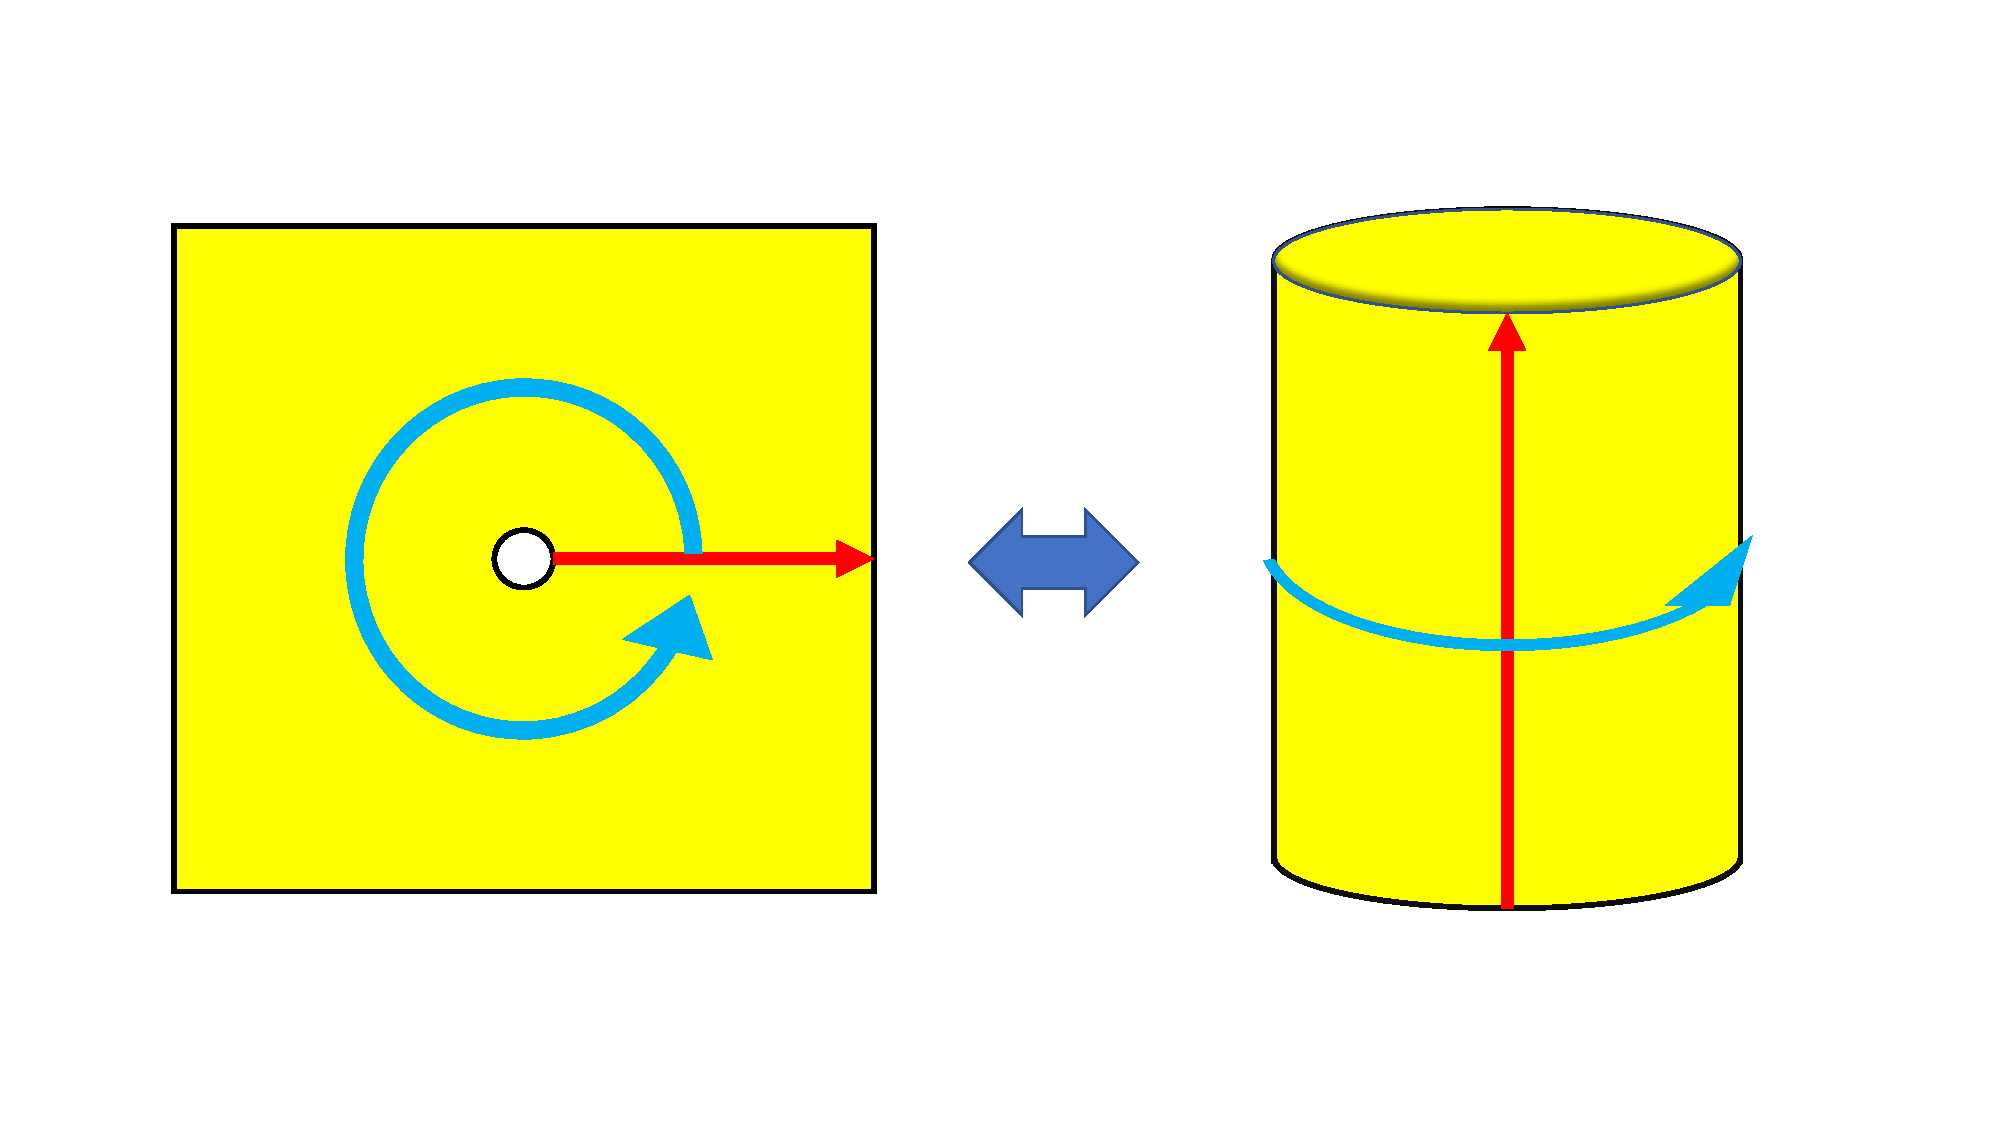
\includegraphics[width=0.7\linewidth]{plane2cylinder.pdf}
	\caption{共形変換$z=e^{-iw}$によって、平面$\C-\{0\}$と円筒$S^1\times \R$が移りあう。平面の動径方向は円筒の時間方向に対応し、平面の角度方向は円筒の円周方向に対応する。}
	\label{fig:plane2cylinder}
\end{figure}

したがって円筒座標でのエネルギー運動量テンソルのLaurant展開係数$L_m^{S^1\times \R}$は平面座標での$L_m$と
\begin{align}
L_m^{S^1\times \R}=L_m-\delta_{m,0} \frac{c}{24}
\end{align}
で関係しており、$L_m^{S^1\times \R}$は交換関係
\begin{align}\label{vircrCylinder}
[L_m^{S^1\times \R},L_n^{S^1\times \R}]=(m-n)L_{m+n}^{S^1\times \R}+\frac{c}{12}m^3\delta_{m+n,0}
\end{align}
を満たす。円筒座標の$\IM w$方向を時間と見なせば、円筒座標$w$での時間並進は平面座標$z$でのスケール変換そのものであり、円筒座標のハミルトニアンは
\begin{align}\label{hamincylinder}
H^{S^1\times \R}&=\oint \frac{dw^1}{2\pi} T_{00}(w)\notag\\
&=L_0^{S^1\times \R}+\overline{L}_0^{S^1\times \R}\\
&=L_0+\overline{L}_0-\frac{c}{12}
\end{align}
となる。

\subsub{ユニタリー共形場理論}
ユニタリー共形場理論(unitary conformal field theory)とは、Virasoro代数の生成子$L_m,\overline{L}_m$が$L_m^\dagger=L_{-m},\overline{L}_m^\dagger=\overline{L}_{-m}$となるような内積$\la\ |\ \ra$を持ったヒルベルト空間に表現された共形場理論のことである。

ユニタリー共形場理論の中心電荷$c$と最高ウェイト$h$は強い制限を受けて、点$(c,h)$は領域$c\geq 1,h\geq 0$にあるか、$0\leq c<1$の離散的な点
\begin{align}
c&=1-\frac{6}{m(m+1)}&&(m=2,3,4,\cdots)\\
h&=\frac{(r(m+1)-sm)^2-1}{4m(m+1)}&&(1\leq r\leq m-1,\ 1\leq s\leq m)
\end{align}
にしか存在しないことが知られている。

とくに中心電荷が$c=1-\frac{6}{m(m+1)}\ (m=2,3,4,\cdots)$となるような、$0\leq c <1$のユニタリー共形場理論を\textbf{ユニタリーミニマル模型}と呼び、$\mathcal{M}_m$で表す。

たとえば中心電荷$c=1/2$の$\mathcal{M}_3$はIsing模型と呼ばれる。これは2次元格子上のIsing模型
\begin{align}
H=-\frac{J}{2}\sum_{i,j} \sigma_i \sigma_j
\end{align}
の臨界点での連続極限に相当する共形場理論になっている。$\mathcal{M}_3$には3つのプライマリー場$1,\varepsilon,\sigma$が存在し、それぞれ共形ウェイト$0,1/2,1/16$を持っている。$1$は恒等演算子である。$\varepsilon,\sigma$はそれぞれエネルギー演算子、スピン演算子と呼ばれ、それぞれ格子上のスピン変数、エネルギーの連続極限に相当する。

\subsection{共形境界条件と二重化のトリック}\label{subsecdoubling}
\begin{oframed}
境界を持った$2$次元Riemann多様体$\Sigma$上の共形場理論を考える。境界$\del\Sigma$の単位接線・法線ベクトルを$t,n$で書くとき、次の境界条件は\textbf{共形境界条件(conformal boundary condition)}と呼ばれる\cite{Cardy:1989ir}。
\begin{align}
T_{\mu\nu} t^\mu n^\nu =0\text{  on }\del \Sigma
\end{align}
複素座標では$n=it,\overline{n}=-i\overline{t}$であり、上の共形境界条件は
\begin{align}
T_{zz}=T_{\overline{z}\overline{z}}\text{  on }\del \Sigma
\end{align}
と書ける。共形境界条件を課した、境界付き多様体上の共形場理論を\textbf{境界共形場理論(boundary conformal field theory, BCFT)}という。
\end{oframed}

共形場理論はスケール変換に対する対称性を持つため、境界つきの空間上での共形場理論の物理量を考える際に、境界条件は非常に重要になる。下で見るように、共形境界条件はVirasoro対称性を半分だけ保つ。高次元共形場理論でも共形境界条件を考えることができるが、そのときも理論の$SO(2,d)$対称性を半分だけ保つ境界条件になっている。

\begin{ex}
上半平面$\UHP$上の共形場理論は実軸を境界として持ち、共形境界条件$T_{zz}(x)=T_{\overline{z}\overline{z}}(x)\ (x\in\R)$を課すことを考える。このとき$T$は実軸上実数をとり、下半平面の点$z$での$T_{zz}(z)$を上半平面の点$\overline{z}$を用いて
\begin{align}
T_{zz}(z)\coloneqq T_{\overline{z}\overline{z}}(\overline{z})=\overline{T_{zz}(\overline{z})}\quad (\IM z<0)
\end{align}
で定めると、Schwartzの鏡像原理から$T$は下半平面へ解析接続される。同様にして$\overline{T}$も下半平面へ反正則に解析接続できる。このようにエネルギー運動量テンソルの解析接続を行う方法は\textbf{二重化のトリック(doubling trick)}と呼ばれる。

上半平面上でのVirasoro代数の生成子$L_m^\UHP$を
\begin{align}
L_m^\UHP\coloneqq \oint_{(\UHP\text{内の半円})}\frac{1}{2\pi i}\left( dz z^{m+1}T(z)-d\overline{z} \overline{z}^{m+1}\overline{T}(\overline{z}) \right)
\end{align}
で定めると、二重化のトリックから半円の積分は$0\in\C$周りの周回積分になり、
\begin{align}
L_m^\UHP&=\oint_{0} \frac{dz}{2\pi i}z^{m+1}T(z)\\
&=-\oint_{0} \frac{d\overline{z}}{2\pi i}\overline{z}^{m+1}\overline{T}(\overline{z})
\end{align}
となる。したがって上半平面では、平面$\C$上のVirasoro代数の生成子$L_m,\overline{L}_m$が共通のものとなり、一つの$L_m^\UHP$のみがVirasoro代数の生成子となる。交換関係は平面$\C$のときと同じで、
\begin{align}
[L_m^\UHP,L_n^\UHP]&=(m-n)L_{m+n}^\UHP+\frac{c}{12}m(m^2-1)\delta_{m+n,0}
\end{align}
である。このことは、上半平面の自己同型群が$PSL(2,\R)$で表されることに対応しており、$L_{-1}^\UHP,L_0^\UHP,L_1^\UHP$がその生成子になっている。
\end{ex}

\subsection{Cardy公式}
最後に、トーラス上の共形場理論がもつモジュラー不変性から、有限温度の円筒上の2次元共形場理論の高エネルギーでの状態密度を記述するCardy公式を導く。

モジュライパラメータ$\tau=\tau_1+i\tau_2$を持ち、$z\sim z+2\pi \sim z+2\pi\tau$となる平坦トーラス$ds^2=dzd\overline{z}$上の共形場理論を考える。トーラスには独立な共形Killingベクトルが$2$つ存在し、それぞれ小円・大円の接線方向への並進変換である。これらの変換に対応する保存量は(\ref{hamincylinder})と同様に
\begin{align}
H^{S^1\times \R}&=L_0^{S^1\times \R}+\overline{L}_0^{S^1\times \R}=L_0+\overline{L}_0-\frac{c}{12}\label{hamtorus}\\
P^{S^1\times \R}&=L_0^{S^1\times \R}-\overline{L}_0^{S^1\times \R}=L_0-\overline{L}_0\label{momtorus}
\end{align}
である。したがってトーラス上の共形場理論の分配関数は
\begin{align}\label{torusPF}
Z_{T^2}(\tau)&=\Tr \exp\left(-2\pi \tau_2 H^{S^1\times \R}+2\pi i \tau_1 P^{S^1\times \R}\right)\\
&=\Tr (e^{2\pi i \tau (L_0-\frac{c}{24})}e^{-2\pi i \overline{\tau} (\overline{L}_0-\frac{c}{24})})
\end{align}
となることが分かる。


平坦トーラスは$\tau$を$PSL(2,\Z)$変換しても共形同値であったから、共形場理論のトーラス分配関数はモジュライパラメータの$PSL(2,\Z)$変換に対する不変性(\textbf{モジュラー不変性})をもち、
\begin{oframed}
\begin{align}
Z_{T^2}(\tau)=Z_{T^2}\left(-\frac{1}{\tau}\right)=Z_{T^2}(\tau+1)
\end{align}
\end{oframed}
を満たすことが要請される。特にモジュライパラメータが純虚数$\tau=i\beta$のときに、$\beta$を系の逆温度と見なすと、分配関数は$\beta\leftrightarrow \beta^{-1}$の変換で不変であり、高温と低温が双対な理論になっていることが分かる。


このモジュラー不変性を使って、ユニタリー共形場理論に対して高温ないし高エネルギー極限でのエントロピーを計算したい。
\subsub{カノニカル分布を用いる方法}
$\tau=i\beta$のときの分配関数は、モジュラー不変性から
\begin{align}
Z_{T^2}(\beta)&=\Tr (e^{-2\pi \beta (L_0+\overline{L}_0-\frac{c}{12})})\\
&=\Tr (e^{-2\pi \beta^{-1} (L_0+\overline{L}_0-\frac{c}{12})})
\end{align}
を満たす。

いまユニタリー共形場理論を考えると$L_0,\overline{L}_0$はエルミート演算子であり、それぞれの最小固有値を$E_0,\overline{E}_0$と書く。このとき$\beta\to 0$の高温極限において分配関数は
\begin{align}
Z_{T^2}(\beta)\sim e^{-2\pi \beta^{-1} (E_0+\overline{E}_0-\frac{c}{12})}
\end{align}
と評価できる。

したがって$\beta\to 0$でのHelmholtz自由エネルギーは
\begin{align}
F(\beta)=-(2\pi\beta)^{-1}\log Z_{T^2}(\beta)\sim \beta^{-2}\left(E_0+\overline{E}_0-\frac{c}{12}\right)
\end{align}
と評価され、同様に熱力学的エントロピーは$\beta\to 0$で
\begin{align}
S_\text{thermal}(\beta)=-\frac{\del F(\beta)}{\del (2\pi\beta)^{-1}}
\sim 4\pi\beta^{-1}\left( \frac{c}{12}-(E_0+\overline{E}_0) \right)
\end{align}
と評価できる。

特に規格化可能で$E_0=\overline{E}_0=0$を満たす真空が存在するようなユニタリー共形場理論については
\begin{oframed}
\begin{align}\label{cardyCE}
S_\text{thermal}(\beta)\sim \frac{c}{3}\pi \beta^{-1}
\end{align}
\end{oframed}
となる。特に高温極限のエントロピーは、理論の詳細によらず中心電荷$c$のみで決まることが分かる。


\subsub{ミクロカノニカル分布を用いる方法}
分配関数$Z_{T^2}(\tau)$を、エネルギー$E+\overline{E}-c/12$での状態密度$\rho(E)\rho(\overline{E})$を用いて
\begin{align}
Z_{T^2}(\tau)=\int_{E_0}^{\infty}dE \rho(E)e^{2\pi i\tau (E-\frac{c}{24})} \int_{\overline{E}_0}^{\infty} d\overline{E} \rho(\overline{E})e^{-2\pi i\overline{\tau}(\overline{E}-\frac{c}{12})}
\end{align}
と表示するとき、Boltzmannエントロピーは
\begin{align}
S_\text{Boltzmann}(E+\overline{E}-c/12)=\log \rho(E)\rho(\overline{E})
\end{align}
で定義される。これを$E,\overline{E}\gg c/24$の高エネルギー極限で漸近評価したい。

状態密度は分配関数の逆Laplace変換で書けて、
\begin{align}
\rho(E)&=\oint d\tau Z(\tau)e^{-2\pi i\tau (E-\frac{c}{24})}
\end{align}
となる。$E_0,\overline{E}_0<c/24$のとき、分配関数は$\tau\sim 0$で$Z_{T^2}(\tau)\sim e^{-2\pi i \tau^{-1} (E_0-\frac{c}{24})}e^{2\pi i \overline{\tau}^{-1} (\overline{E}_0-\frac{c}{24})}
$と特異性を持つので、上の逆Laplace変換を
\begin{align}
\rho(E)\sim \oint d\tau \exp\left(-2\pi i \left(\tau (E-\frac{c}{24})+\tau^{-1}(E_0-\frac{c}{24}) \right) \right)
\end{align}
と評価できる。$E\gg c/24$の高エネルギー極限で上の積分を鞍点法で近似すると、鞍点は
\begin{align}
\tau_\ast =i\sqrt{\frac{c/24-E_0}{E-c/24}}
\end{align}
と決まり、
\begin{align}
\rho(E)\sim \exp\left( 2\pi\sqrt{\left(\frac{c}{6}-4E_0\right)\left(E-\frac{c}{24}\right)} \right)
\end{align}
と評価できる。この密度行列の漸近評価式は\textbf{Cardy公式(Cardy formula)}\cite{Cardy:1991kr}と呼ばれる。

したがって$E,\overline{E}\gg c/24$の高エネルギー極限でのBoltzmannエントロピーは
\begin{align}
S_\text{Boltzmann}(E+\overline{E}-c/12)\sim 2\pi\sqrt{\left(\frac{c}{6}-4E_0\right)\left(E-\frac{c}{24}\right)}+2\pi\sqrt{\left(\frac{c}{6}-4\overline{E}_0\right)\left(\overline{E}-\frac{c}{24}\right)}
\end{align}
と評価できる。

特に規格化可能で$E_0=\overline{E}_0=0$を満たす真空が存在するようなユニタリー共形場理論については
\begin{oframed}
\begin{align}\label{cardyMCE}
S_\text{Boltzmann}(E+\overline{E}-c/12)\sim 2\pi\sqrt{\frac{c}{6}\left(E-\frac{c}{24}\right)}+2\pi\sqrt{\frac{c}{6}\left(\overline{E}-\frac{c}{24}\right)}
\end{align}
\end{oframed}
となる。特に高エネルギー極限のエントロピーは、理論の詳細によらず中心電荷$c$のみで決まることが分かる。


\section{2次元零質量自由スカラー場}\label{sec:2dscalar}
ここでは\ref{sec:2dcft}で導入した2次元共形場理論の具体例として、2次元零質量自由スカラー場の頂点演算子の相関関数を計算する。2次元零質量自由スカラー場は、弦理論で重要な役割を果たすPolyakov作用に現れ、頂点演算子とは外線の閉弦に対応する演算子である。したがって以下で計算する相関関数は、弦理論の相関関数の計算にも応用できる。

\subsection{頂点演算子}
\subsub{正規順序}
以下では2次元平面上の零質量自由実スカラー場$X(z,\overline{z})$の理論を考える。
\begin{oframed}
\begin{align}
S[X]_{\C}=\frac{1}{8\pi}\int_\C d^2 x \del^\mu X \del_\mu X=\frac{1}{4\pi}\int_\C d^2 z \del X \overline{\del} X
\end{align}
\end{oframed}

運動方程式は波動方程式$\la \del\overline{\del}X \ra_\C=0$であり、解は正則・反正則な部分$X_L,X_R$に分解できる。
\begin{align}
X(z,\overline{z})=X_L(z)+X_R(\overline{z})
\end{align}

平面上の2点グリーン関数$G(z,\overline{z})=\la X(z,\overline{z})X(0,0)\ra_\C$はラプラシアンの積分核$-\laplacian G(z,\overline{z})=2\pi\delta(z,\overline{z})$であり、
\begin{align}
G(z,\overline{z})=-\log|z|^2
\end{align}
となる。つまり場$X$の挿入点が近づくとき、相関関数は$\log$発散する。

この$\log$発散の正則化として、\textbf{正規順序(normal order)}$\colon \ \colon $を
\begin{align}
\colon X(z,\overline{z})X(0,0)\colon \coloneqq X(z,\overline{z})X(0,0)+\log|z|^2
\end{align}
で定める\footnote{この定義は、$X$の生成消滅演算子の順番を並べ替えるものとして定義した正規順序に一致する。}。一般の$X$の汎関数$F[X]$の正規順序はWick縮約をとって
\begin{align}
\colon F[X](z,\overline{z})\colon =\exp\left(\frac{1}{2}\int d^2 z_1 d^2 z_2 \log|z_1-z_2|^2 \frac{\delta}{\delta X(z_1,\overline{z}_1)}\frac{\delta}{\delta X(z_2,\overline{z}_2)} \right)F[X](z,\overline{z})
\end{align}
で定義する。このとき正規順序化された2つの演算子$\colon F[X]\colon ,\colon G[X]\colon $の積は
\begin{align}
\colon F[X]\colon \colon G[X]\colon =\exp\left( -\int d^2 z_1 d^2 z_2 \log|z_1-z_2|^2 \frac{\delta}{\delta X_F(z_1,\overline{z}_1)}\frac{\delta}{\delta X_G(z_2,\overline{z}_2)} \right)\colon F[X]G[X]\colon 
\end{align}
となることに注意する。ただし$\delta/\delta X_F,\delta/\delta X_G$はそれぞれ$F[X],G[X]$に対する汎関数微分を表している。

\subsub{エネルギー運動量テンソル}
エネルギー運動量テンソルは正規順序をとって
\begin{align}
T_{\mu\nu}&=-\frac{1}{2}\colon \left(\del_{\mu}X\del_{\nu}X-\frac{1}{2}\eta_{\mu\nu}\del_{\rho}X\del^{\rho}X\right)\colon \\
T&=-\frac{1}{2}\colon \del X_L\del X_L\colon \\
\overline{T}&=-\frac{1}{2}\colon \overline{\del} X_R\overline{\del} X_R\colon 
\end{align}
で定義する。このとき$TT$の演算子積展開の発散項は
\begin{align}
T(z)T(0)&=\frac{1}{4}\colon \del X_L(z)\del X_L(z)\colon \colon \del X_L(0)\del X_L(0)\colon \\
&=\frac{1}{4}\exp\left(-\int dz_1 dz_2 \log(z_1-z_2) \frac{\delta}{\delta X_{L,T}(z_1)}\frac{\delta}{\delta X_{L,V}(z_2)} \right)\notag\\
&\qquad \colon \del X_L(z)\del X_L(z)\colon \colon \del X_L(0)\del X_L(0)\colon \\
&\sim \frac{1}{2z^4}+\frac{2}{z^2}T(0)+\frac{1}{z}\del T(0)
\end{align}
となる。よって2次元零質量自由スカラー場の中心電荷は$c=1$である。

\subsub{頂点演算子}
$V_{(k_L,k_R)}(z,\overline{z})\coloneqq \colon e^{ik_L X_L(z)+ik_R X_R(\overline{z})}\colon $で定義された演算子$V_{(k_L,k_R)}$を\textbf{頂点演算子(vertex operator)}という。とくに$k_L=k_R=k$のときの頂点演算子を$\colon e^{ikX(z,\overline{z})}\colon $と書く。

頂点演算子とエネルギー運動量テンソルの発散項は
\begin{align}
T(z)V_{(k_L,k_R)}(0,0)&=-\frac{1}{2}\colon \del X_L(z)\del X_L(z)\colon \colon e^{ik_L X_L(0)+ik_R X_R(\overline{0})}\colon \\
&=-\frac{1}{2}\exp\left(-\int dz_1 dz_2 \log(z_1-z_2) \frac{\delta}{\delta X_{L,T}(z_1)}\frac{\delta}{\delta X_{L,V}(z_2)} \right)\notag\\
&\qquad \colon \del X_L(0)\del X_L(0)e^{ik_L X_L(0)+ik_R X_R(\overline{0})}\colon \\
&\sim \frac{k_L^2/2}{z^2}V_{(k_L,k_R)}(0,0)+\frac{ik_L}{z}\colon \del X_L(0)e^{ik_L X_L(0)+ik_R X_R(\overline{0})}\colon 
\end{align}
となるから、$V_{(k_L,k_R)}$はウェイト$(k_L^2/2,k_R^2/2)$のプライマリー場になる。

また、頂点演算子同士の演算子積展開の発散項は
\begin{align}\label{vertexopOPE}
V_{(k_{L1},k_{R1})}(z,\overline{z})V_{(k_{L2},k_{R2})}(0,0)\sim z^{k_{L1}k_{L2}}\overline{z}^{k_{R1}k_{R2}} V_{(k_{L1}+k_{L2},k_{R1}+k_{R2})}
\end{align}
となることに注意しておく。

\subsection{共形境界条件と二重化のトリック}
境界を持ったリーマン面$\Sigma$上の零質量自由スカラー場を考える。共形境界条件は、境界での単位接線・法線ベクトルを$t,n$として
\begin{align}
0=T_{\mu\nu}t^\mu n^\nu=(t^\mu \del_{\mu}X)(n^\nu \del_{\nu} X) \text{   on }\del\Sigma
\end{align}
となる。そこで例えばスカラー場$X$の境界条件として、
\begin{align}
&&&\text{Neumann境界条件}&& n^\mu \del_{\mu}X=0\ \text{ on }\del\Sigma &&\\
&&&\text{Dirichlet境界条件}&& t^\mu \del_{\mu}X=0\ \text{ on }\del\Sigma \iff X=(\text{const}) \text{ on }\del\Sigma &&
\end{align}
を考えると、これらは共形境界条件になっている。

\begin{ex}
いま上半平面$\UHP$の境界である実軸上で$X$にNeumann境界条件
\begin{align}
\del X_L(x)=\overline{\del} X_R(x),\ (x\in\R)
\end{align}
を課すときを考える。(\ref{subsecdoubling})でのエネルギー運動量テンソルに対する二重化のトリックと同様に、スカラー場$X$についての二重化のトリック
\begin{align}
X_L(z)\coloneqq X_R(\overline{z})\ (\IM z<0)
\end{align}
を施すことで、$X_L$は下半平面へ解析接続される。同様に$X_R$は下半平面へ反正則に解析接続される。
\end{ex}

\subsection{頂点演算子の相関関数}
\subsub{グリーン関数の一般論}
以下では連結コンパクトRiemann面$(\Sigma,g)$上の零質量自由実スカラー場$X(z,\overline{z})$の理論を考える。$\Sigma$上の2点関数$\la X(x_1,\tau_1)X(x_2,\tau_2) \ra_\Sigma$はラプラシアンの積分核として与えられる。これを計算するためにまず場$X(x,\tau)$を$(\Sigma,g)$のラプラシアン$\laplacian$の固有関数で展開する。$-\laplacian$の固有値を$0=\omega_0<\omega_1<\omega_2<\cdots$として、各$\omega_i$に対応する固有空間の正規直交基底を$X_{i,I_i}$とする。とくにゼロモードはただ一つの基底を持つので単に$X_0$と書く\footnote{Hodge理論の結果から、向き付け可能連結コンパクトRiemann多様体の$-\laplacian$は、離散的で非有界で集積点を持たない非負のスペクトルをもち、各固有空間は有限次元で、線形独立な固有ベクトル全体は$L^2$空間の完全系を張ることが知られている。また、ラプラシアンのゼロモードの独立なベクトルの数はコホモロジーの次元に一致することも知られている。したがって$0$次形式のゼロモードの基底はただ一つ存在し、それは定数関数に他ならない。}。
\begin{align}
X(x,\tau)&=\sum_{i=0}^\infty\sum_{I_i} a_{i,I_i} X_{i,I_i}(x,\tau)\\
\laplacian X_{i,I_i}&=-\omega_i^2 X_{i,I_i}\\
\int_\Sigma d^2 x X_{i,I_i} X_{j,J_j} &= \delta_{ij}\delta_{I_i,J_j}\\
X_0&=\left(\int_\Sigma d^2 x \right)^{-1/2}=(\Sigma\text{の面積})^{-1/2}
\end{align}

2点関数$\la X(x_1,\tau_1)X(x_2,\tau_2) \ra_\Sigma$を経路積分から計算するために、$X$と結合する外場$J$を加えた分配関数$Z[J]=\la \exp\left( i\int_\Sigma d^2 x J(x,\tau)X(x,\tau) \right) \ra_\Sigma$を考える。

外場$J$の$X_{i,I_i}$成分を$J_{i,I_i}=\int_\Sigma d^2 x J(x,\tau)X_{i,I_i}(x,\tau)$とすれば、
\begin{align}\label{generalpartitionfunc}
Z_\Sigma[J]&=\int \mathcal{D}X \exp \left( \int_\Sigma(\frac{1}{8\pi}X\laplacian X+iJX)  \right)\notag\\
&=\prod_{i,I_i}\int da_{i,I_i}\exp\left( -\frac{\omega_{i,I_i}^2}{8\pi}a_{i,I_i}^2+iJ_{i,I_i}a_{i,I_i} \right)\notag\\
&=\int da_0\exp(ia_0 J_0)\prod_{i\neq 0, I_i}\int da_{i,I_i}\exp\left( -\frac{\omega_{i,I_i}^2}{8\pi}\left(a_{i,I_i}-i\frac{4\pi}{\omega_{i,I_i}^2}J_{i,I_i}\right)^2-\frac{2\pi}{\omega_{i,I_i}^2}J_{i,I_i}^2 \right)\notag\\
&=i(2\pi)^2\delta^2(J_0)\prod_{i\neq 0,I_i}\left(\sqrt{\frac{\pi}{\omega_{i,I_i}^2/8\pi}}\right)^2 \exp\left(-\frac{2\pi}{\omega_{i,I_i}^2}J_{i,I_i}^2\right)\notag\\
&=i(2\pi)^2\delta^2(J_0)\times \left(\text{det}' \frac{-\laplacian}{8\pi^2} \right)^{-1} \exp\left( \frac{1}{2}\int d^2 x_1 d^2 x_2 J(x_1,\tau_1)J(x_2,\tau_2)G'(x_1,\overline{x_1};x_2,\tau_2) \right)
\end{align}
と表示できる。ここで、$\text{det}'$は$0$を除く固有値の無限積を表す。また、途中で$i$倍が生じたのはEuclid化のためである。

$G'(x_1,\tau_1;x_2,\tau_2)$は次で定義される。
\begin{align}
G'(x_1,\tau_1;x_2,\tau_2)=\sum_{i\neq 0,I_i}\frac{4\pi}{\omega_{i,I_i}^2}X_{i,I_i}(x_1,\tau_1)X_{i,I_i}(x_2,\tau_2)
\end{align}
これはゼロモードの寄与を除いたGreen関数であり、次を満たす。
\begin{align}\label{greenfunc}
-\frac{1}{4\pi}\laplacian|_{(x_1,\tau_1)}G'(x_1,\overline{x_1};x_2,\tau_2)=\delta^2(x_1-x_2,\tau_1-\tau_2)-X_0^2 
\end{align}

一般的な分配関数をGreen関数で書き直したので、次に頂点演算子の$N$点関数を考える。

正則化されていない頂点演算子$e^{ik_i X(x_i,\tau_i)}$の挿入は外場$J(x,\tau)=k_i \delta^2(x-x_i,\tau-\tau_i)$の挿入に等しく、(\ref{generalpartitionfunc})から、
\begin{align}
\la \prod_{i=1}^{N} e^{ikX(x_i,\tau_i)} \ra_\Sigma&=i(2\pi)^2\delta^2\left(\sum_{i=1}^{N}k_i \right)X_0^{-2}\left(\text{det}' \frac{-\laplacian}{8\pi^2} \right)^{-1}\notag\\
&\quad \times \exp\left( -\sum_{\substack{i,j=1\\i<j}}^{N}k_i k_j G'(x_i,\tau_i;x_j,\tau_j)-\frac{1}{2}\sum_{i=1}^{N}k_i^2 G'(x_i,\tau_i;x_i,\tau_i) \right)
\end{align}
となる。いま、自己相互作用項の$G'(x_i,\tau_i;x_i,\tau_i)$は発散するので、次のように正則化する。
\begin{align}
G_r'(x_1,\tau_1;x_2,\tau_2)=G'(x_1,\tau_1;x_2,\tau_2)+\log d^2((x_1,\tau_1),(x_2,\tau_2))
\end{align}
ただし$d((x_1,\tau_1),(x_2,\tau_2))$は$\Sigma$上の2点$(x_1,\tau_1),(x_2,\tau_2)$の測地距離を表す。この正則化は、平面では正規順序をとることに一致する。

この正則化のもとで、頂点演算子$N$点関数は
\begin{oframed}
\begin{align}\label{vertexnptfunc}
\la \prod_{i=1}^{N} \colon e^{ikX(x_i,\tau_i)}\colon  \ra_\Sigma&=i(2\pi)^2\delta\left(\sum_{i=1}^{N}k_i \right)X_0^{-2}\left(\text{det}' \frac{-\laplacian}{8\pi^2} \right)^{-1}\notag\\
&\quad \times \exp\left( -\sum_{\substack{i,j=1\\i<j}}^{N}k_i k_j G'(x_i,\tau_i;x_j,\tau_j)-\frac{1}{2}\sum_{i=1}^{N}k_i^2 G_r'(x_i,\tau_i;x_i,\tau_i) \right)
\end{align}
\end{oframed}
となる。

以下ではこの式の具体例として、球面、平面、上半平面、トーラス、有限の長さの円筒での頂点演算子$N$点関数を計算する。

\subsub{球面・平面での相関関数}
球面$S^2$あるいは平面$\C$に無限遠点を付け加えてコンパクト化した空間上に等温座標$(z,\overline{z})$をとり、計量を$ds_\omega^2=e^{2\omega(z,\overline{z})}dzd\overline{z}$と表す\footnote{一意化定理から$S^2$に微分同相なRiemann多様体はすべて共形同値になる。つまり、どのような$\omega$をとっても$ds_\omega^2$は、$\R^3$に埋め込まれた半径$1$の球面の計量$ds^2=d\theta^2+\sin^2 \theta d\phi^2$に共形同値である。}。

(\ref{greenfunc})の解は、
\begin{align}
G'(z_1,\overline{z_1};z_2,\overline{z}_2)&=-\log (|z_1-z_2|^2)+f(z_1,\overline{z}_1)+f(z_2,\overline{z}_2)-k\\
f(z,\overline{z})&=\frac{X_0^2}{2}\int_\Sigma d^2 w \exp(2\omega(w,\overline{w}))\log (|z-w|^2)
\end{align}
となる。ただし定数$k$は$G'$と$X_0$を直交させるように決まり、$-\log (|z_1-z_2|^2)+f(z_1,\overline{z}_1)+f(z_2,\overline{z}_2)$の定数部分に他ならない。

このとき$G_r'$は
\begin{align}
G_r'(z,\overline{z};z,\overline{z})&=-\log(|z-z|^2)+2f(z,\overline{z})-k+\log(e^{2\omega(z,\overline{z})}|z-z|^2)\notag\\
&=2f(z,\overline{z})+2\omega(z,\overline{z})-k
\end{align}
となる。これを(\ref{vertexnptfunc})に代入すると、運動量保存$\delta\left(\sum_{i=1}^{N}k_i \right)$から$f(z,\overline{z})$と$k$の寄与は消えて、
\begin{align}
\la \prod_{i=1}^{N} \colon e^{ikX(z_i,\overline{z}_i)}\colon  \ra_{S^2}&=i(2\pi)^2\delta\left(\sum_{i=1}^{N}k_i \right)X_0^{-2}\left(\text{det}' \frac{-\laplacian}{8\pi^2} \right)^{-1}\notag\\
&\quad \times \exp\left( -\sum_{i=1}^{N}k_i^2\omega(z_i,\overline{z}_i) \right)\prod_{\substack{i,j=1\\i<j}}^{N}|z_i-z_j|^{2k_ik_j}
\end{align}
となる。特に$S^2$として、平面$\C$に無限遠点を加えてコンパクト化したものを考える場合、曲率を無限遠方に押し付けるのが自然で、全ての頂点演算子の挿入点を含む領域で$\omega$が$0$になるような計量をとる。このとき頂点演算子$N$点関数は
\begin{align}\label{vertexnptSphere}
\la \prod_{i=1}^{N} \colon e^{ikX(z_i,\overline{z}_i)}\colon  \ra_{\C}&=i(2\pi)^2\delta\left(\sum_{i=1}^{N}k_i \right)X_0^{-2}\left(\text{det}' \frac{-\laplacian}{8\pi^2} \right)^{-1}\notag\\
&\quad \times \prod_{\substack{i,j=1\\i<j}}^{N}|z_i-z_j|^{2k_ik_j}
\end{align}
となる。
\begin{figure}[h]
	\centering
	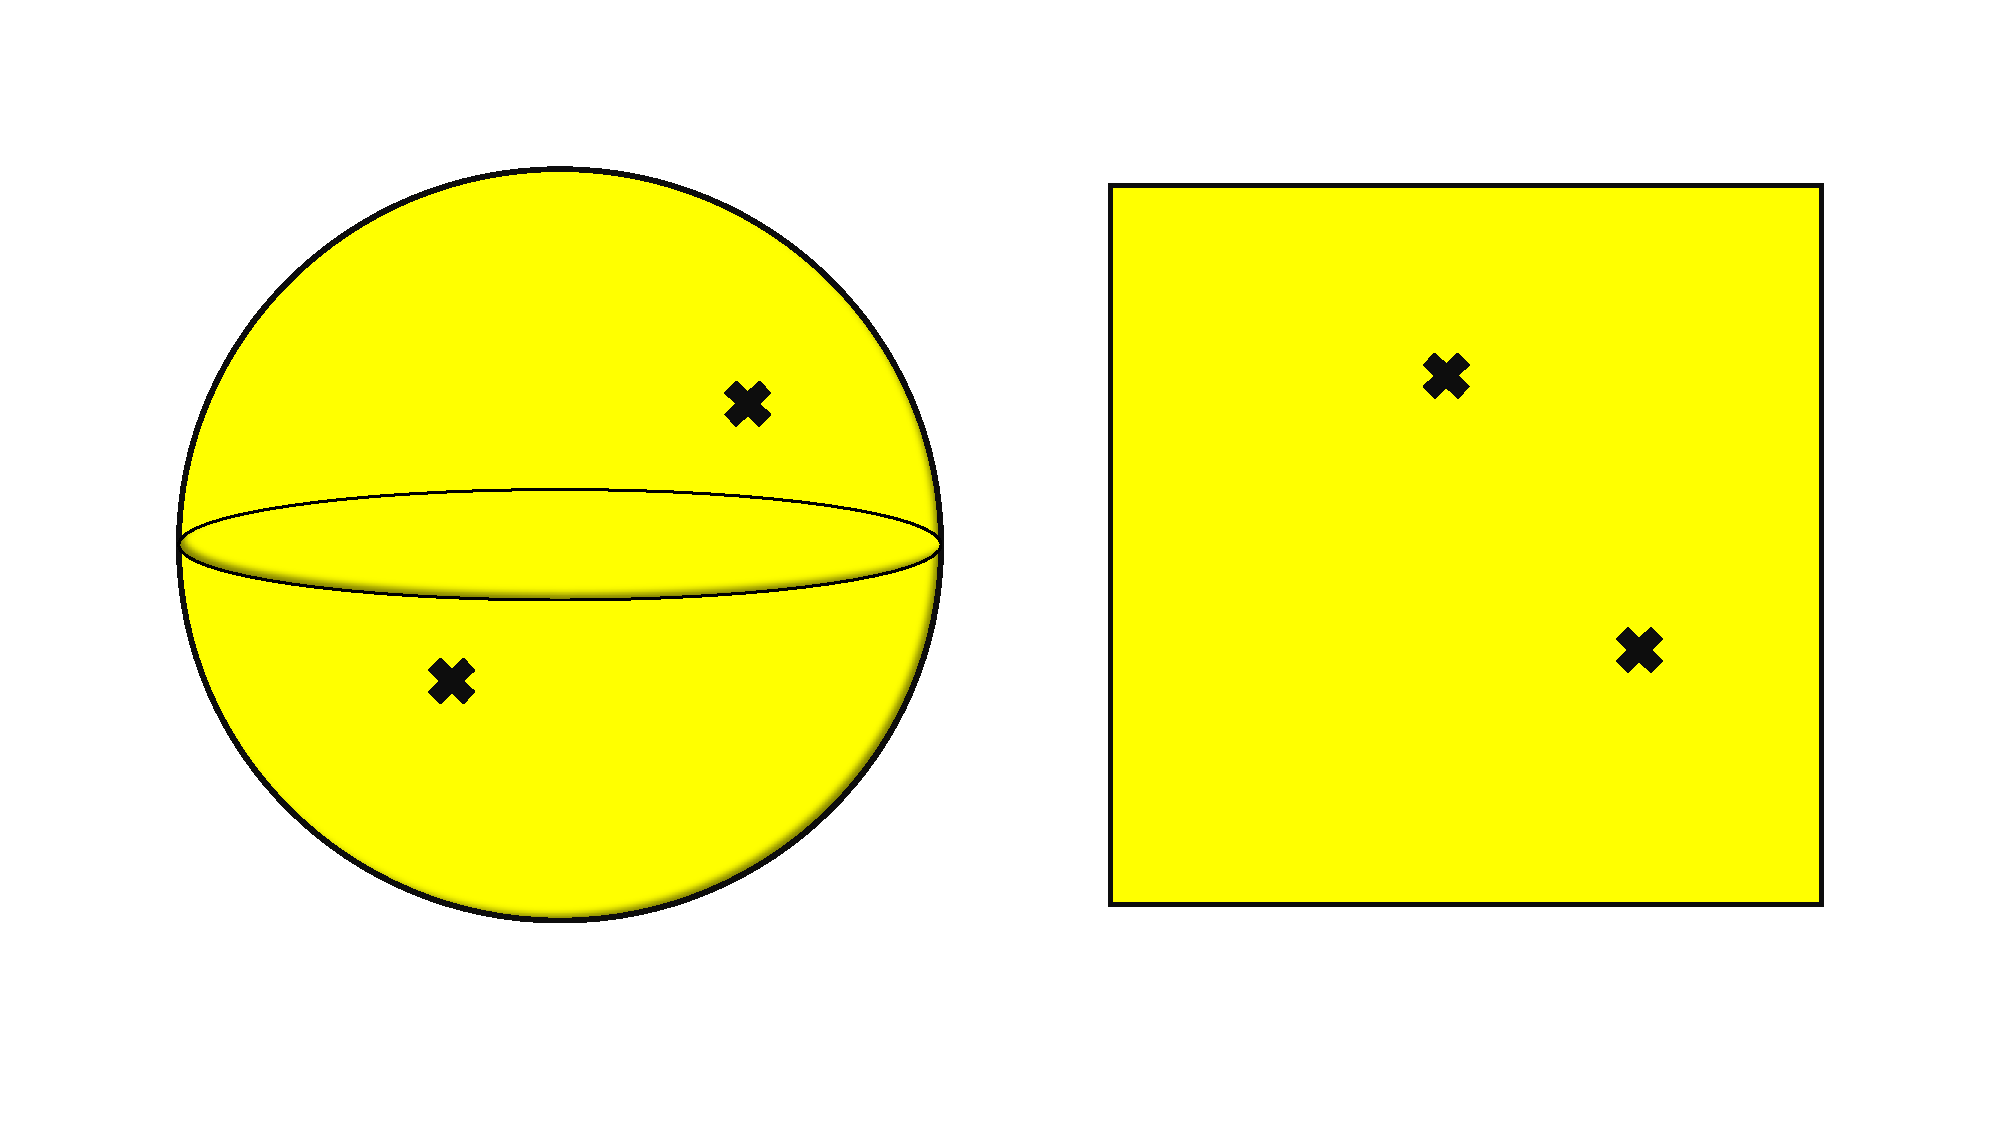
\includegraphics[width=0.7\linewidth]{sphereCF.pdf}
	\caption{バツ($\times$)印は球面や平面に挿入された頂点演算子を表している。}
	\label{fig:spherecf}
\end{figure}


\subsub{上半平面での相関関数}
上半平面の実軸上でNeumannまたはDirichlet境界条件を課して、二重化のトリックを使う。このとき$X_L(z)$と$X_R(\overline{z})$が同一視されたことにより、$(z,\overline{z})$の鏡像$(\overline{z},z)$の寄与がGreen関数に生じる。また、無限遠点をコンパクト化して曲率を無限遠に押し付ける。

鏡像の寄与によりGreen関数は
\begin{align}\label{scalarGreenUHP}
G'(z_1,\overline{z_1};z_2,\overline{z}_2)&=-\log (|z_1-z_2|^2)\mp\log(|z_1-\overline{z}_2|^2)+(\text{運動量保存で消える項})\\
G_r'(z,\overline{z};z,\overline{z})&=\mp\log(|z-\overline{z}|^2)+(\text{運動量保存で消える項})
\end{align}
となる。ただし$\mp$の負符号がNeumann境界条件、正符号がDirichlet境界条件に対応している。したがって例えばNeumann境界条件に対しての相関関数は、
\begin{align}
\la \prod_{i=1}^{N} \colon e^{ikX(z_i,\overline{z}_i)}\colon  \ra_{\UHP}&=i(2\pi)^2\delta\left(\sum_{i=1}^{N}k_i \right)X_0^{-2}\left(\text{det}' \frac{-\laplacian}{8\pi^2} \right)^{-1}\notag\\
&\quad \times \prod_{i=1}^{N}|z_i-\overline{z}_i|^{k_i^2} \prod_{\substack{i,j=1\\i<j}}^{N}|z_i-z_j|^{2k_ik_j}|z_i-\overline{z}_j|^{2k_ik_j}
\end{align}
となる。
\begin{figure}[h]
	\centering
	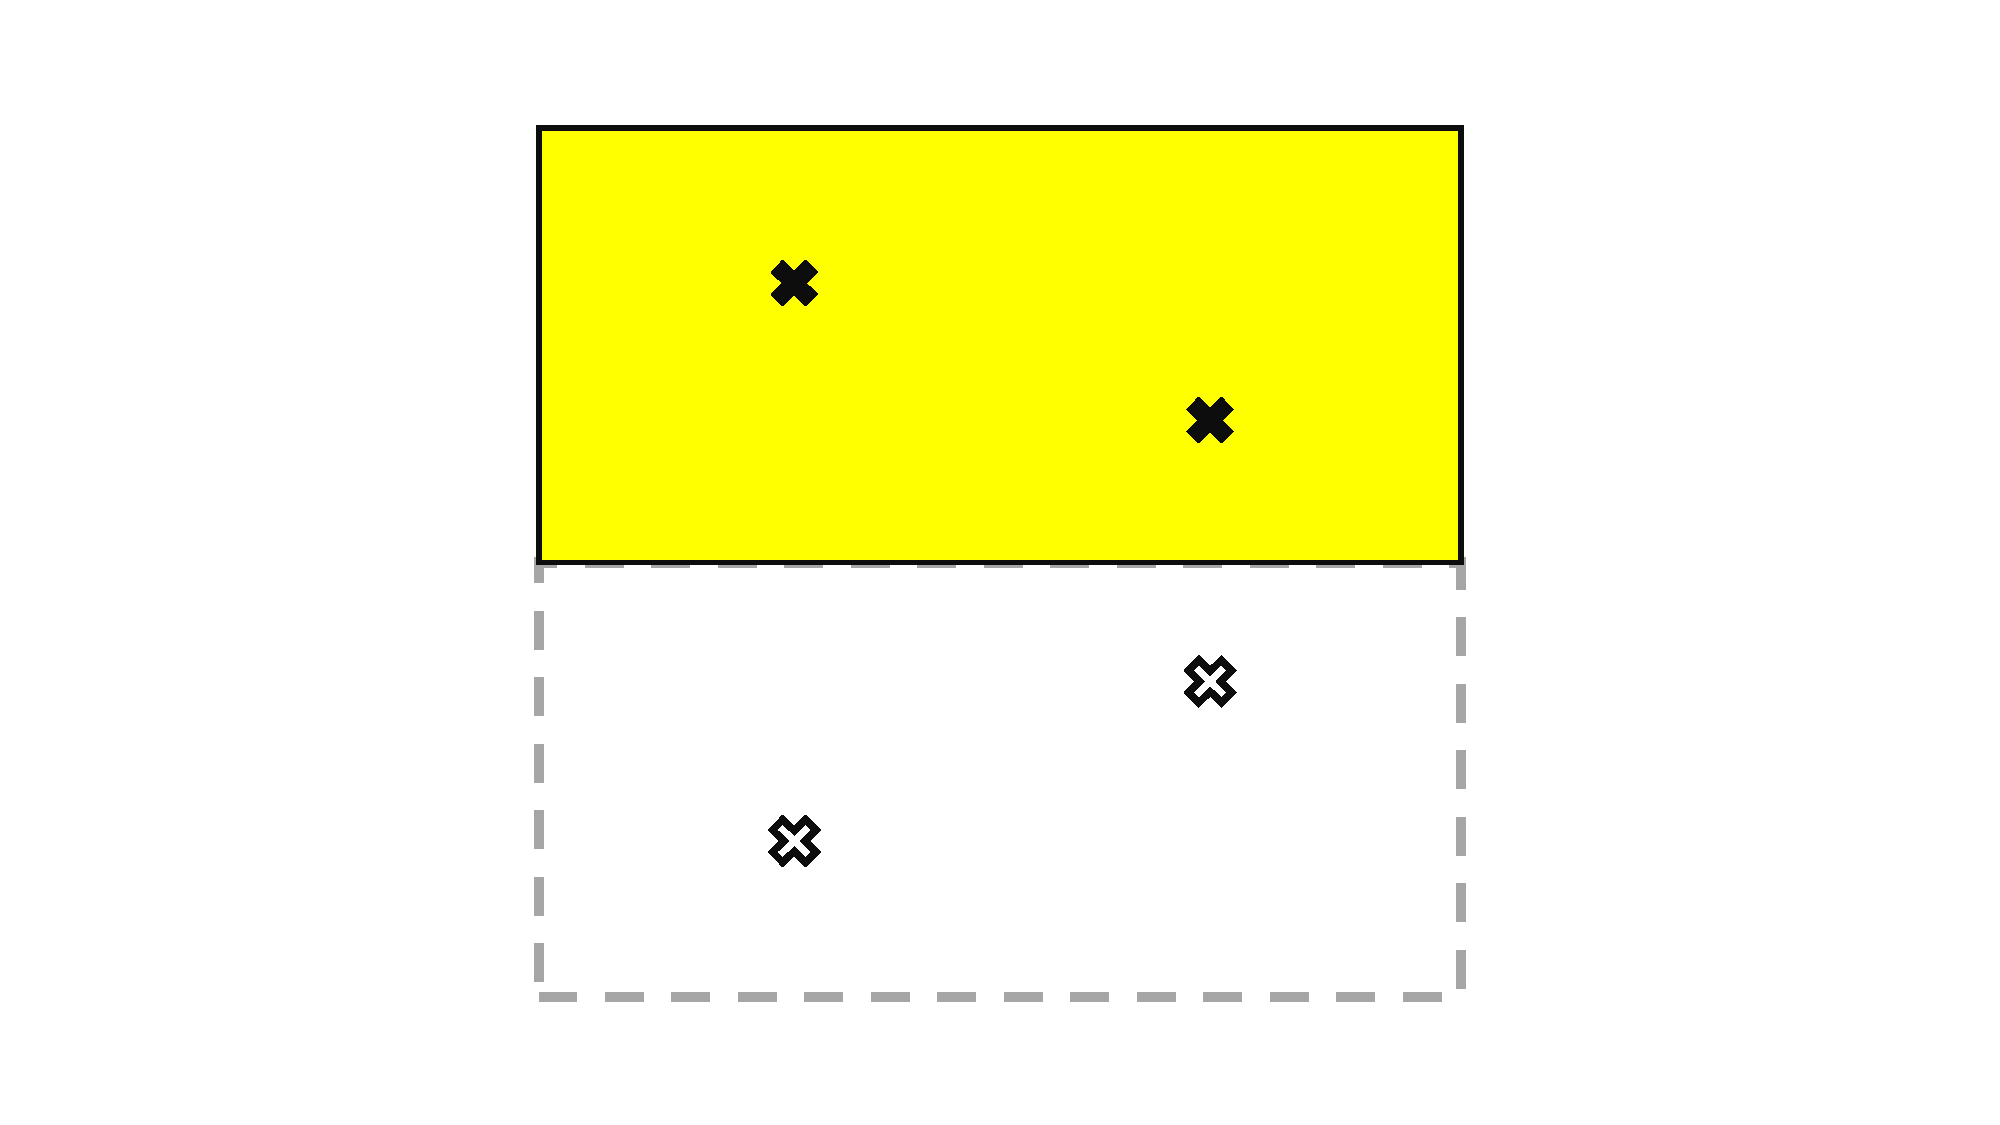
\includegraphics[width=0.7\linewidth]{UHPCF.pdf}
	\caption{黒いバツ($\times$)印は上半平面に挿入された頂点演算子を表している。下半平面にある白いバツ印は、二重化のトリックによって生じた鏡像を表している。}
	\label{fig:uhpcf}
\end{figure}


\subsub{トーラスでの相関関数}
モジュライパラメータ$\tau=\tau_1+i\tau_2$を持ち、$z\sim z+2\pi \sim z+2\pi\tau$となる平坦トーラス$ds^2=dzd\overline{z}$上のスカラー場を考えると、$X_0=(4\pi^2\tau_2)^{-1/2}$であり、グリーン関数は(\ref{greenfunc})から次のように決まる。

\begin{align}
G'(z_1,\overline{z_1};z_2,\overline{z}_2)&=-\log \left(\left|\theta_1(\frac{z_1-z_2}{2\pi}|\tau) \right|^2\right)+\frac{(\IM(z_1-z_2) )^2}{2\pi\tau_2}-k(\tau,\overline{\tau})\\
\theta_1(\nu|\tau)&=-\sum_{n=-\infty}^{\infty}\exp\left(\pi i\left(n+\frac{1}{2}\right)^2\tau+2\pi i\left(n+\frac{1}{2}\right)\left(\nu+\frac{1}{2}\right)\right)\\
&=2e^{\pi i \tau/4}\sin\pi\nu \prod_{k=1}^{\infty}(1-e^{2\pi i k\tau})(1-e^{2\pi i\nu}e^{2\pi i k\tau})(1-e^{-2\pi i\nu}e^{2\pi i k\tau})
\end{align}

ただし定数$k(\tau,\overline{\tau})$は$G'$と$X_0$を直交させるように決まる。第$2$項の$\IM$は、テータ関数$\theta_1$の擬二重周期性(\ref{quasidoubleperiod})を補正して、$G'$をトーラス上の$1$価関数にするために現れている。

また$G_r'$は
\begin{align}
G'(z,\overline{z};z,\overline{z})&=-\log \left(\left|\theta_1(\frac{z-z}{2\pi}|\tau) \right|^2\right)+\frac{(\IM(z-z) )^2}{2\pi\tau_2}-k(\tau,\overline{\tau})+\log(|z-z|^2)\notag\\
&=-\log\left(\left|\eta(\tau)^3\right|^2\right)-k(\tau,\overline{\tau})
\end{align}
であり、これを(\ref{vertexnptfunc})に代入すると、運動量保存$\delta\left(\sum_{i=1}^{N}k_i \right)$から$k(\tau,\overline{\tau})$の寄与は消える。さらに運動量保存のもとで$\frac{1}{2}\sum_i k_i^2=-\sum_{i<j}k_ik_j$が成り立つから、
\begin{align}
\la \prod_{i=1}^{N} \colon e^{ikX(z_i,\overline{z}_i)}\colon  \ra_{T^2}&=i(2\pi)^2\delta\left(\sum_{i=1}^{N}k_i \right)X_0^{-2}\left(\text{det}' \frac{-\laplacian}{8\pi^2} \right)^{-1}\notag\\
&\quad \times \prod_{\substack{i,j=1\\i<j}}^{N}\left|\frac{\theta_1(\frac{z_i-z_j}{2\pi}|\tau)}{\eta(\tau)^3}\exp\left(-\frac{(\IM(z_i-z_j) )^2}{4\pi\tau_2}\right) \right|^{2k_ik_j}
\end{align}
を得る。
\begin{figure}[h]
	\centering
	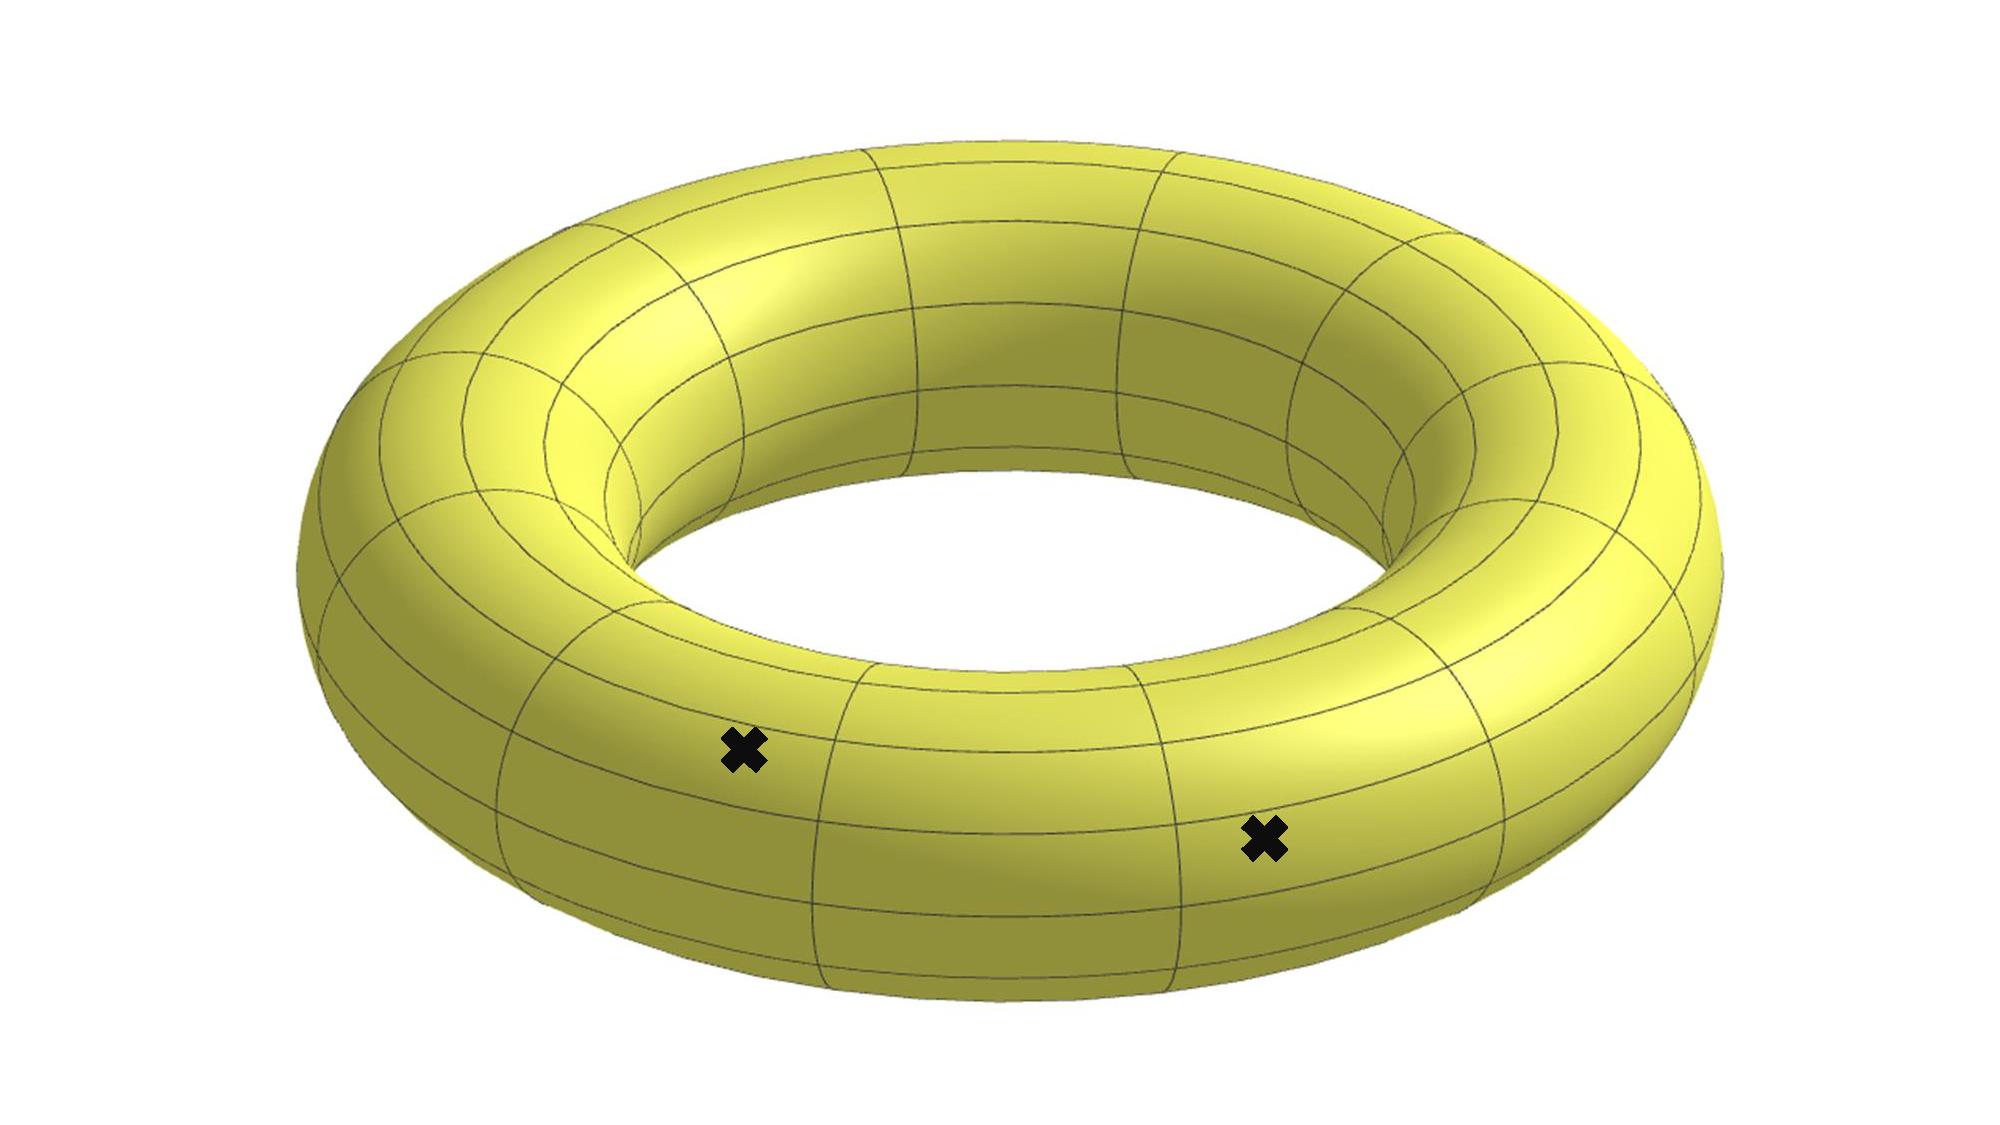
\includegraphics[width=0.7\linewidth]{torusCF.pdf}
	\caption{バツ($\times$)印はトーラスに挿入された頂点演算子を表している。}
	\label{fig:toruscf}
\end{figure}


\subsub{有限の長さの円筒での相関関数}
後の\ref{chap:doublequench}章への応用を考えて、$\RE z=-\pi/2,\pi/2$に境界をもち、$z\sim z+2\pi i\beta$と同一視の入った円筒$[-\pi/2,\pi/2]\times S_{\beta}^1$ (図\ref{fig:cylindercf})を考える。境界でNeumann境界条件またはDirichlet境界条件を課して二重化のトリックを使えば、モジュライパラメータ$i\beta$を持ち$z\sim z+2\pi \sim z+2\pi i\beta$となる平坦トーラスへ解析接続される。$(z,\overline{z})$の鏡像は
\begin{align}
(z',\overline{z}')=(\pi-\overline{z},\pi-z)
\end{align}
にあり、グリーン関数は
\begin{align}\label{scalarGreenCylinder}
G'(z_1,\overline{z_1};z_2,\overline{z}_2)&=-\log \left(\left|\theta_1(\frac{z_1-z_2}{2\pi}|i\beta) \right|^2\right)\mp\log \left(\left|\theta_1(\frac{z_1-z_2'}{2\pi}|i\beta) \right|^2\right)\notag\\
&\quad +\frac{(\IM(z_1-z_2) )^2}{2\pi\beta}\pm\frac{(\IM(z_1-z_2') )^2}{2\pi\beta}+(\text{運動量保存で消える項})\\
&=-\log \left(\left|\theta_1(\frac{z_1-z_2}{2\pi}|i\beta) \right|^2\right)\mp\log \left(\left|\theta_2(\frac{z_1+\overline{z}_2}{2\pi}|i\beta) \right|^2\right)\notag\\
&\quad +\frac{(\IM(z_1-z_2) )^2}{2\pi\beta}\pm\frac{(\IM(z_1+\overline{z}_2) )^2}{2\pi\beta}+(\text{運動量保存で消える項})\\
G_r'(z,\overline{z};z,\overline{z})&=-\log\left(\left|\frac{\del_\nu\theta_1(0|\tau)}{2\pi}\right|^2\right)\mp\log \left(\left|\theta_2(\frac{z+\overline{z}}{2\pi}|\tau) \right|^2\right)\notag\\
&\quad +(\text{運動量保存で消える項})
\end{align}
である。ただし$\mp$の負符号がNeumann境界条件、正符号がDirichlet境界条件に対応している。

例えばNeumann境界条件についての頂点演算子の$N$点関数は
\begin{align}
&\la \prod_{i=1}^{N} \colon e^{ikX(z_i,\overline{z}_i)}\colon  \ra_{[-\pi/2,\pi/2]\times S_\beta^1}\notag\\
&=i(2\pi)^2\delta\left(\sum_{i=1}^{N}k_i \right)X_0^{-2}\left(\text{det}' \frac{-\laplacian}{8\pi^2} \right)^{-1}\notag\\
&\quad \times \prod_{\substack{i,j=1\\i<j}}^{N}\left|\frac{\theta_1(\frac{z_i-z_j}{2\pi}|i\beta)}{\eta(i\beta)^3}\theta_2(\frac{z_i+\overline{z}_j}{2\pi}|i\beta)\exp\left(-\frac{(\IM (z_i-z_j) )^2}{2\pi\beta}\right) \right|^{2k_ik_j}\times \prod_{i=1}^{N}\left|\theta_2(\frac{z_i+\overline{z}_i}{2\pi}|i\beta)\right|^{k_i^2}
\end{align}
となる。
\begin{figure}[h]
	\centering
	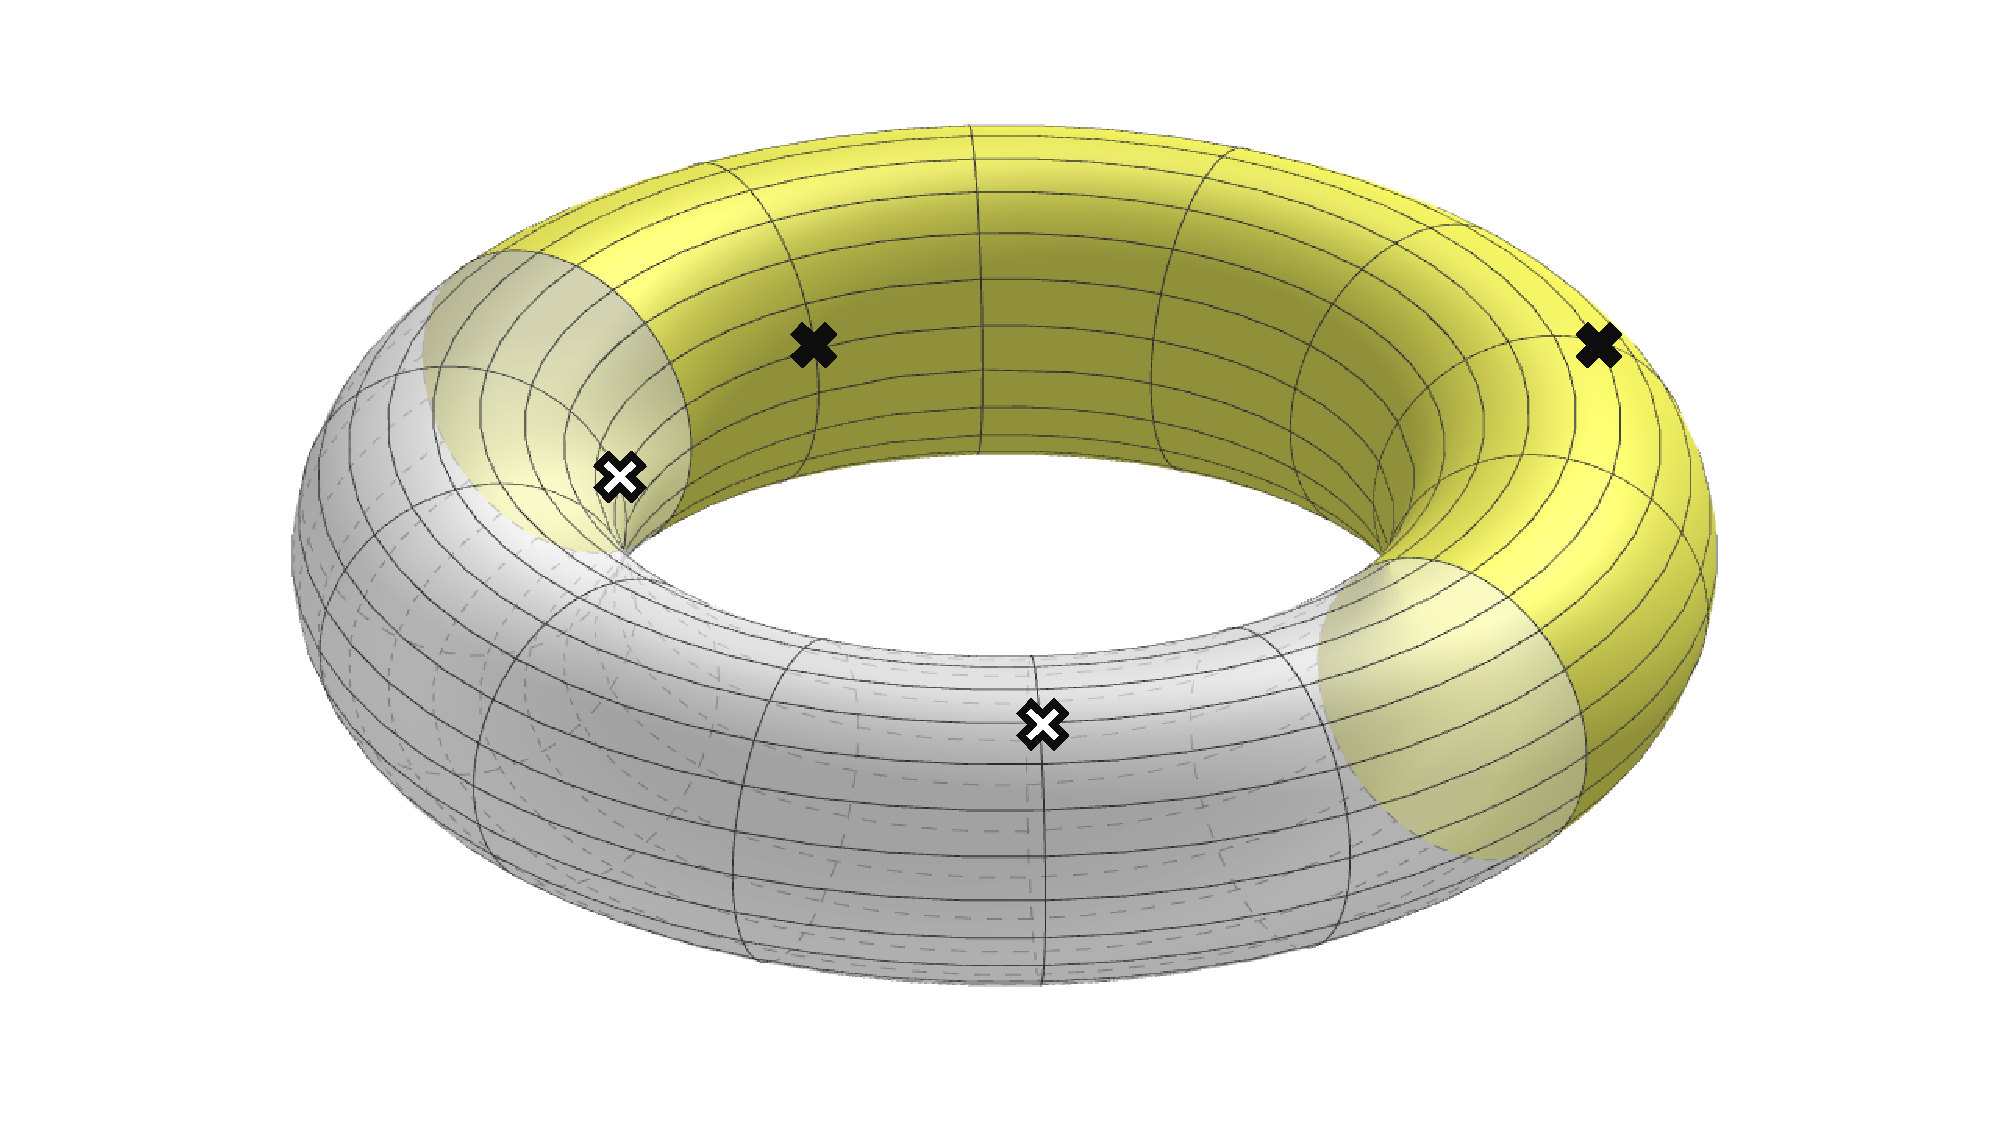
\includegraphics[width=0.7\linewidth]{cylinderCF.pdf}
	\caption{$\RE z=-\pi/2,\pi/2$に境界をもち、$z\sim z+2\pi i\beta\  (\beta<1)$と同一視の入った円筒$[-\pi/2,\pi/2]\times S_{\beta}^1$に対する二重化のトリックの概略図。黒いバツ($\times$)印は有限の長さの円筒に挿入された頂点演算子を表している。白いバツ印は、二重化のトリックによって生じた鏡像を表している。}
	\label{fig:cylindercf}
\end{figure}


\subsub{正則・反正則部分でウェイトが異なる場合}
上の計算では、正則・反正則部分のウェイトが等しい場合$\colon e^{ikX(z,\overline{z})}\colon $を考えた。一般の頂点演算子$\colon e^{ik_L X_L(z)+ik_R X_R(\overline{z})}\colon $の$N$点関数は上の結果とほとんど同じものになる。具体的には、次の変更をすればよい。

球面・平面・上半平面の場合には以下の変更をすればよい。
\begin{align}
|z_i-z_j|^{2k_ik_j}&\to (z_i-z_j)^{k_{Li}k_{Lj}}(\overline{z}_i-\overline{z}_j)^{k_{Ri}k_{Rj}}\\
|z_i-\overline{z}_j|^{2k_ik_j}&\to (z_i-\overline{z}_j)^{k_{Li}k_{Rj}}(\overline{z}_i-z_j)^{k_{Ri}k_{Lj}}\\
|z_i-\overline{z}_i|^{k_i^2}&\to |z_i-\overline{z}_i|^{k_{Li}k_{Ri}}
\end{align}
トーラス・有限サイズシリンダーの場合には、$F_{i}(z)=\theta_{i}(\frac{z}{2\pi}|i\beta)\exp(-\frac{(\IM(z))^2}{4\pi\beta})\ (i=1,2)$と書くと、
\begin{align}
|F_1(z_i-z_j)|^{2k_ik_j}&\to F_1(z_i-z_j)^{k_{Li}k_{Lj}}(F_1(\overline{z}_i-\overline{z}_j))^{k_{Ri}k_{Rj}}\\
|F_2(z_i+\overline{z}_j)|^{2k_ik_j}&\to F_2(z_i+\overline{z}_j)^{k_{Li}k_{Rj}}F_2(\overline{z}_i+z_j)^{k_{Ri}k_{Lj}}\\
|F_2(z_i+\overline{z}_i)|^{k_i^2}&\to |F_2(z_i+\overline{z}_i)|^{k_{Li}k_{Rj}}
\end{align}
と変更すればよい。

\begin{ex}
2次元零質量自由ディラック場のエンタングルメントエントロピーの計算で用いる式を導出しておく。

$(k_L,k_R)=(k,-k)$のときの頂点演算子$V_{(k,-k)}(z,\overline{z})=\colon e^{ik (X_L(z)- X_R(\overline{z}))}\colon $の2点関数で、境界のある場合はNeumann境界条件をとったものを計算する。球面、平面、上半平面、トーラス、有限・無限に長い円筒において定数部分を除いて以下のようになる。
\begin{oframed}
\begin{description}
	\item[球面・平面]
	\begin{align}
	\la V_{(k,-k)}(z_1,\overline{z_1}) V_{(-k,k)}(z_2,\overline{z_2}) \ra_{S^2,\C} \propto \left(\frac{1}{(z_1-z_2)(\overline{z}_1-\overline{z}_2)}\right)^{k^2}
	\end{align}
	
	\item[上半平面]
	\begin{align}
	\la V_{(k,-k)}(z_1,\overline{z_1}) V_{(-k,k)}(z_2,\overline{z_2}) \ra_{D^2} \propto \left(\frac{(z_1-\overline{z}_2)(\overline{z}_1-z_2)}{(z_1-z_2)(\overline{z}_1-\overline{z}_2)(z_1-\overline{z}_1)(z_2-\overline{z}_2)}\right)^{k^2}
	\end{align}
	
	\item[トーラス] \hfill\\
	$\overline{\theta_1(\nu|i\beta)}=-\theta_1(-\overline{\nu}|i\beta)$と$\eta(i\beta)\in\R$に注意すると、モジュライパラメーターが純虚数のときの$2$点関数は次のようになる。
	\begin{align}
	\la V_{(k,-k)}(z_1,\overline{z_1}) V_{(-k,k)}(z_2,\overline{z_2}) \ra_{T^2} \propto \left(\frac{\eta(i\beta)^6}{\theta_1(\frac{z_1-z_2}{2\pi}|i\beta)\theta_1(\frac{\overline{z}_1-\overline{z}_2}{2\pi}|i\beta)}e^{\frac{(\IM(z_1-z_2) )^2}{2\pi\beta}}\right)^{k^2}
	\end{align}
	
	\item[有限の長さの円筒]
	\begin{align}
	&\la V_{(k,-k)}(z_1,\overline{z_1}) V_{(-k,k)}(z_2,\overline{z_2}) \ra_{[-\pi/2,\pi/2]\times S_\beta^1}\notag\\
	&\propto \left(\frac{\eta(i\beta)^6}{\theta_1(\frac{z_1-z_2}{2\pi}|i\beta)\theta_1(\frac{\overline{z}_1-\overline{z}_2}{2\pi}|i\beta)}
	\frac{\theta_2(\frac{z_1+\overline{z}_2}{2\pi}|i\beta)\theta_2(\frac{\overline{z}_1+z_2}{2\pi}|i\beta)}{\theta_2(\frac{z_1+\overline{z}_1}{2\pi}|i\beta)\theta_2(\frac{z_2+\overline{z}_2}{2\pi}|i\beta)}\right)^{k^2}\label{fincylvertex2ptfunc}
	\end{align}
	
	\item[無限に長い円筒] \hfill\\
	トーラス上の相関関数で、実軸方向の周期を$2\pi$から$2\pi L$に変換して、$\beta\to\infty$の極限をとれば、半径$L$の無限に長い円筒$S_L^1\times \R$上の相関関数を得る。
	\begin{align}
	\la V_{(k,-k)}(z_1,\overline{z_1}) V_{(-k,k)}(z_2,\overline{z_2}) \ra_{S_L^1\times \R} \propto \left(\frac{1}{4L^2\sin\frac{z_1-z_2}{2L}\sin\frac{\overline{z}_1-\overline{z}_2}{2L}}\right)^{k^2}
	\end{align}
\end{description}
\end{oframed}

またこれらの2点関数の結果は、$(k_L,k_R)=(k,k)$のときの頂点演算子$V_{(k,k)}(z,\overline{z})=$\\$\colon e^{ik (X_L(z)+ X_R(\overline{z}))}\colon $の2点関数で、境界のある場合はDirichlet境界条件をとったものに等しいことにも注意しておく。
\end{ex}

\subsection{分配関数}
\subsub{トーラス分配関数}
スカラー場のトーラス分配関数は(\ref{generalpartitionfunc})や(\ref{torusPF})を計算すればよく、どちらでも同じ結果を得る。ここでは(\ref{generalpartitionfunc})を計算してみる。

まず平坦トーラスの座標$w$として$w\sim w+2\pi \sim w+2\pi\tau$の同一視が入ったものを考えて、$w=\xi_1+\tau\xi_2,\overline{w}=\xi_1+\overline{\tau}\xi_2$で$\xi_1,\xi_2$を定義すると、$X$を
\begin{align}
X&=\sum_{m,n\in\Z} X_{m,n}e^{i(m\xi_1+n\xi_2)}\\
&=\sum_{m,n\in\Z} X_{m,n}\exp\left( \frac{n-m\overline{\tau}}{2\tau_2}w-\frac{n-m\tau}{2\tau_2}\overline{w} \right)
\end{align}
とモード展開できる。ただし$X$は実スカラー場なので$X_{m,n}=\overline{X_{-m,-n}}$の条件がついている。

固有モード$e^{i(m\xi_1+n\xi_2)}$は
\begin{align}
\int_{T^2} d^2 w e^{-i(m\xi_1+n\xi_2)}e^{i(m'\xi_1+n'\xi_2)}=4\pi^2\tau_2 \delta_{m,m'}\delta_{n,n'}
\end{align}
を満たす直交系になっている。したがって、(\ref{generalpartitionfunc})の分配関数で外場$J$を$0$としたものは
\begin{align}
Z_{T^2}&=\frac{\int \mathcal{D}X \exp \left( \int_\Sigma(\frac{1}{8\pi}X\laplacian X)\right)}{\text{ゼロモードの寄与}}\\
&=\left({\det}' \frac{-\laplacian}{8\pi^2}\times 4\pi^2\tau_2 \right)^{-1}\\
&=\left( \prod_{m,n\in\Z-\{(0,0)\}} \frac{|n-m\tau|^2}{8\pi^2 \tau_2^2}\times 4\pi^2\tau_2 \right)^{-1/2}\label{freebosontoruspartitionfunctiontotyuukeisann}\\
&=\left(\prod_{n=1}^{\infty} \frac{n^2}{2\tau_2} \right)^{-1}\left( \prod_{m=1}^{\infty}\prod_{n\in \Z} \frac{|n-m\tau|^2}{2\tau_2} \right)^{-1}
\end{align}
となる。ただし(\ref{freebosontoruspartitionfunctiontotyuukeisann})で$1/2$乗になったのは$X_{m,n}=\overline{X_{-m,-n}}$の条件があるためである。


無限積を$\zeta$関数正則化を用いて評価すれば、最終的にトーラス分配関数
\begin{align}
Z_{T^2}(\tau)=\frac{1}{\sqrt{8\pi^2 \tau_2} |\eta(\tau)|^2}
\end{align}
を得る。$\tau_2|\eta(\tau)|^4$はモジュラー不変であり、$Z_{T^2}$はたしかにモジュラー不変になっている。


\subsub{円筒分配関数}
$2$つの境界で同じ共形境界条件を課した有限の長さの円筒の分配関数も同様に(\ref{generalpartitionfunc})や(\ref{torusPF})を計算できて、どちらでも同じ結果を得る。

円筒の座標を$w=x+i\tau,\  w\sim w+2\pi i\beta,\  -\pi/2\leq x \leq \pi/2$とすると、このときモジュライパラメータは純虚数$\tau=i\beta$である。

$2$つの境界$x=\pm \pi/2$での境界条件として
\begin{itemize}
	\item ともにNeumann境界条件
	\item ともにDirichlet境界条件$X(x=\pm\pi\beta/2)=x_{\pm}$
	\item 一方がNeumann境界条件で、もう一方はDirichlet境界条件
\end{itemize}
を課したとき、それぞれの円筒分配関数は
\begin{align}
Z_{[-\pi/2,\pi/2]\times S_\beta^1,\text{NN}}(i\beta)&=\frac{1}{\sqrt{16\pi^2 \beta} \eta(i\beta)}\\
Z_{[-\pi/2,\pi/2]\times S_\beta^1,\text{DD}}(i\beta)&=\frac{\exp\left(-\frac{(x_+-x_-)^2}{4\pi}\beta\right)}{\eta(i\beta)}\\
Z_{[-\pi/2,\pi/2]\times S_\beta^1,\text{ND}}(i\beta)&=\sqrt{\frac{\eta(i\beta)}{\theta_4(0|i\beta)}}
\end{align}
となる。

上の分配関数はいずれもモジュラー不変ではなく、さらに高温・低温極限$\beta\to 0,\infty$での漸近的な振る舞いも異なる。これは共形場理論がスケール対称性を持つことから、系の性質が境界条件に強く依存することが表れている。

\section{2次元零質量自由Dirac場}\label{sec:2ddirac}
ここでは\ref{sec:2dcft}で導入した2次元共形場理論の2つ目の具体例として、2次元零質量自由Dirac場について解説する。2次元零質量自由Dirac場は、ボソン化と呼ばれる対応関係によって2次元零質量自由スカラー場の理論に等価になる。このボソン化の手法は、2次元零質量自由Dirac場に対するエンタングルメントエントロピーの計算でも重要な役割を果たす。

\subsection{理論の定義}
2次元平面上の零質量自由Dirac場$\psi(z,\overline{z})$の理論を考える。
\begin{align}
S[X]_{\C}=\frac{1}{4\pi}\int_{\C} d^2 x \overline{\Psi}\gamma^\mu\del_\mu\Psi
\end{align}
ここで、ガンマ行列$\gamma^0,\gamma^1$は
\begin{align}
\gamma^0=\left(\begin{array}{cc}
0 & 1 \\
-1 & 0 \end{array}
\right),\ \gamma^1=\left(\begin{array}{cc}
0 & 1 \\
1 & 0 \end{array}
\right)
\end{align}
で定義している。また、$\del_t=-i\del_\tau$とユークリッド化して、
\begin{align}
\Psi=\left(\begin{array}{c}
\tilde{\psi} \\
\psi \end{array}
\right),\ \overline{\Psi}=\left(\begin{array}{c}
\overline{\psi} \\
\overline{\tilde{\psi}}\end{array}
\right)
\end{align}
と$2$つのWeylスピノルに分解すれば、作用は
\begin{oframed}
\begin{align}
S[X]_{\C}=\frac{1}{4\pi}\int_{\C} d^2 z (\overline{\psi}\overline{\del}\psi+\overline{\tilde{\psi}}\del\tilde{\psi})
\end{align}
\end{oframed}
となる。

運動方程式は$\overline{\del}\psi=0=\overline{\del}\overline{\psi},\ \del\tilde{\psi}=0=\del\overline{\tilde{\psi}}$であり、$\overline{\psi}\psi, \overline{\tilde{\psi}}\tilde{\psi}$の演算子積展開は
\begin{align}
\overline{\psi}(z)\psi(0)\sim \frac{1}{z},\quad \overline{\tilde{\psi}}(\overline{z})\tilde{\psi}(0)\sim \frac{1}{\overline{z}}
\end{align}
となる。

エネルギー運動量テンソルは
\begin{align}
T&=\frac{1}{2}\left((\del\overline{\psi})\psi-\overline{\psi}\del\psi\right)\\
\overline{T}&=\frac{1}{2}\left((\overline{\del}\overline{\tilde{\psi}})\tilde{\psi}-\overline{\tilde{\psi}}\overline{\del}\tilde{\psi}\right)
\end{align}
であり、$TT,T\psi$の演算子積展開は
\begin{align}
T(z)T(0)&\sim \frac{1}{2z^4}+\frac{2}{z^2}T(0)+\frac{1}{z}\del T(0)\\
T(z)\psi(0)&\sim \frac{1}{2z^2}\psi(0)+\frac{1}{z}\del\psi(0)
\end{align}
となる。したがって2次元零質量自由Dirac場は中心電荷$c=1$の共形場理論であり、場$\psi,\overline{\psi}$は共形ウェイト$(1/2,0)$のプライマリー場になる。同様に場$\tilde{\psi},\overline{\tilde{\psi}}$は共形ウェイト$(0,1/2)$のプライマリー場になる。

\subsection{スピン構造}
一般に、向き付け可能Riemann多様体$M$上にスピン構造(spin structure)が入るなら、その個数は$H_1(M,\Z_2)$の元の個数で与えられる。例えば、$d$次元平面$\R^d$、$d$次元球面$S^d$や、種数$g$のコンパクトRiemann面$\Sigma_g$にはつねにスピン構造を入れることができ、その個数はそれぞれ
\begin{align}
\R^d\text{に入るスピン構造の数}&=1\\
S^1\text{に入るスピン構造の数}&=2\\
S^d\ (d\geq 2)\text{に入るスピン構造の数}&=1\\
\Sigma_g\text{に入るスピン構造の数}&=2^{2g}
\end{align}
である。

したがって空間方向がコンパクト化された円筒上のDirac場の理論を考えると、$S^1\times \R=\{(x,\tau)\mid x\sim x+2\pi \}$には$2$個のスピン構造が入るので、場$\psi$が$x$方向に一周したときの境界条件として、
\begin{oframed}
\begin{align}
&&&\textbf{NSセクター(Neveu-Schwartz sector)}&\Psi(x+2\pi,\tau)&=-\Psi(x,\tau)&&\\
&&&\textbf{Rセクター(Ramond sector)}&\Psi(x+2\pi,\tau)&=\Psi(x,\tau)&&
\end{align}
\end{oframed}
と、$2$つの境界条件を考えることができる。

とくに平面上のDirac場を有限温度化して、時間方向がコンパクト化された円筒$\R\times S^1=\{(x,\tau)\mid \tau\sim \tau+\beta\}$上の経路積分を考える場合、フェルミオンの反可換性から、時間方向には反周期境界条件(=NSセクター)を課す必要がある。

また、空間方向がコンパクト化された円筒$w=x+i\tau,\ x\sim x+2\pi$上の零質量自由ディラック場を共形変換$z=e^{-iw}$で平面$\C-\{0\}$に移したとき、$\psi,\tilde{\psi}$が共形ウェイト$1/2$のプライマリー場であることからNS/Rセクターの境界条件が
\begin{align}
&&&\text{NSセクター}&\Psi(e^{2\pi i}z,e^{-2\pi i}\overline{z})&=\Psi(z,\overline{z})&&\\
&&&\text{Rセクター}&\Psi(e^{2\pi i}z,e^{-2\pi i}\overline{z})&=-\Psi(z,\overline{z})&&
\end{align}
となって、$-1$倍の付き方が逆になることに注意する。

\subsection{ボソン化}
平面$\C-\{0\}$上の2次元零質量自由スカラー/Dirac場を比べてみると、中心電荷はともに$c=1$で、さらにスカラー場の頂点演算子$V_{(1,0)}$とフェルミオン場$\psi,\overline{\psi}$の共形ウェイトはともに$(1/2,0)$である。
\begin{oframed}
特にNSセクターのフェルミオン場と頂点演算子は、$0$周りに一周したときの境界条件も同じで、相関関数が同じになるという意味で
\begin{align}
\psi(z)&\simeq \colon e^{iX_L(z)} \colon\\
\overline{\psi}(z)&\simeq \colon e^{-i X_L(z)} \colon\\
\tilde{\psi}(\overline{z})&\simeq \colon e^{iX_R(\overline{z})} \colon\\
\overline{\tilde{\psi}}(\overline{z})&\simeq \colon e^{-i X_R(\overline{z})} \colon
\end{align}
という等価関係が成り立っている。つまり、NSセクターのフェルミオンの相関関数は、対応する頂点演算子の相関関数として計算しても同じ結果を得る。この対応はボソン・フェルミオン対応と呼ばれ、上の式により$\psi$を$:e^{iX}:$に対応づけることを\textbf{ボソン化(bosonization)}という。
\end{oframed}

\subsection{分配関数}
\subsub{トーラス分配関数}
2次元零質量自由Dirac場のトーラス分配関数を計算する。まずスピン構造について注意しておくと、円筒に入るスピン構造の数は$2$個だったのに対し、トーラスでは$4$個入る。これはトーラスが$T^2=S^1\times S^1$であり、小円・大円方向にそれぞれ独立にNS/Rセクターの境界条件をつけることができるためである。

したがってトーラスの座標を$w=x+i\tau,\ w\sim w+2\pi\sim w+2\pi\tau$とすると、
\begin{align}
&&&\textbf{NS-NSセクター}&\Psi(w+2\pi)&=-\Psi(w)&\Psi(w+2\pi\tau)&=-\Psi(w)&&\\
&&&\textbf{NS-Rセクター}&\Psi(w+2\pi)&=-\Psi(w)&\Psi(w+2\pi\tau)&=\Psi(w)&&\\
&&&\textbf{R-NSセクター}&\Psi(w+2\pi)&=\Psi(w)&\Psi(w+2\pi\tau)&=-\Psi(w)&&\\
&&&\textbf{R-Rセクター}&\Psi(w+2\pi)&=\Psi(w)&\Psi(w+2\pi\tau)&=\Psi(w)&&
\end{align}
という$4$つのスピン構造が入る。

各セクターでのトーラス分配関数はスカラー場の場合と同様に、$\psi$と$\tilde{\psi}$のモードを足し上げて計算できて、
\begin{align}
Z_\text{NS-NS}(\tau)&=\left| \frac{\theta_3(0|\tau)}{\eta(\tau)} \right|^2\\
Z_\text{NS-R}(\tau)&=\left| \frac{\theta_4(0|\tau)}{\eta(\tau)} \right|^2\\
Z_\text{R-NS}(\tau)&=\left| \frac{\theta_2(0|\tau)}{\eta(\tau)} \right|^2\\
Z_\text{R-R}(\tau)&=0=\left| \frac{\theta_1(0|\tau)}{\eta(\tau)} \right|^2
\end{align}
となる。

これらの分配関数はモジュラー不変ではないが、スピン構造をすべて足し上げたもの
\begin{align}
Z_{T^2}(\tau)&=\frac{1}{2}\left(Z_\text{NS-NS}(\tau)+Z_\text{NS-R}(\tau)+Z_\text{R-NS}(\tau)+Z_\text{R-R}(\tau)\right)\notag\\
&=\frac{1}{2}\left( \left| \frac{\theta_3(0|\tau)}{\eta(\tau)} \right|^2+\left| \frac{\theta_4(0|\tau)}{\eta(\tau)} \right|^2+\left| \frac{\theta_2(0|\tau)}{\eta(\tau)} \right|^2 \right)
\end{align}
はモジュラー不変な分配関数になる。

\subsub{円筒分配関数}
円筒の座標を$w=x+i\tau,\  w\sim w+2\pi i\beta,\  -\pi/2\leq x \leq \pi/2$とする。モジュライパラメータは純虚数$\tau=i\beta$であり、$2$つの境界$x=\pm \pi/2$でともに$\psi,\tilde{\psi}$のNeumann境界条件をとる。この円筒の上のNSセクターのDirac場の分配関数を計算する。

いま$z=ie^{-iw}$の共形変換をつかって、円筒を上半平面上のバウムクーヘン型の領域(図\ref{fig:cyl2uhp})に移して二重化のトリックを使う。このとき上半平面を原点中心に一周するときに周期境界条件がつくので、トーラス上に二重化されたDirac場はNS-NSセクターのスピン構造をもつ。さらに、円筒上の場$\psi,\tilde{\psi}$は二重化により共通のものとなり、トーラス上の場は$\psi$のみ現れる。
\begin{figure}[h]
	\centering
	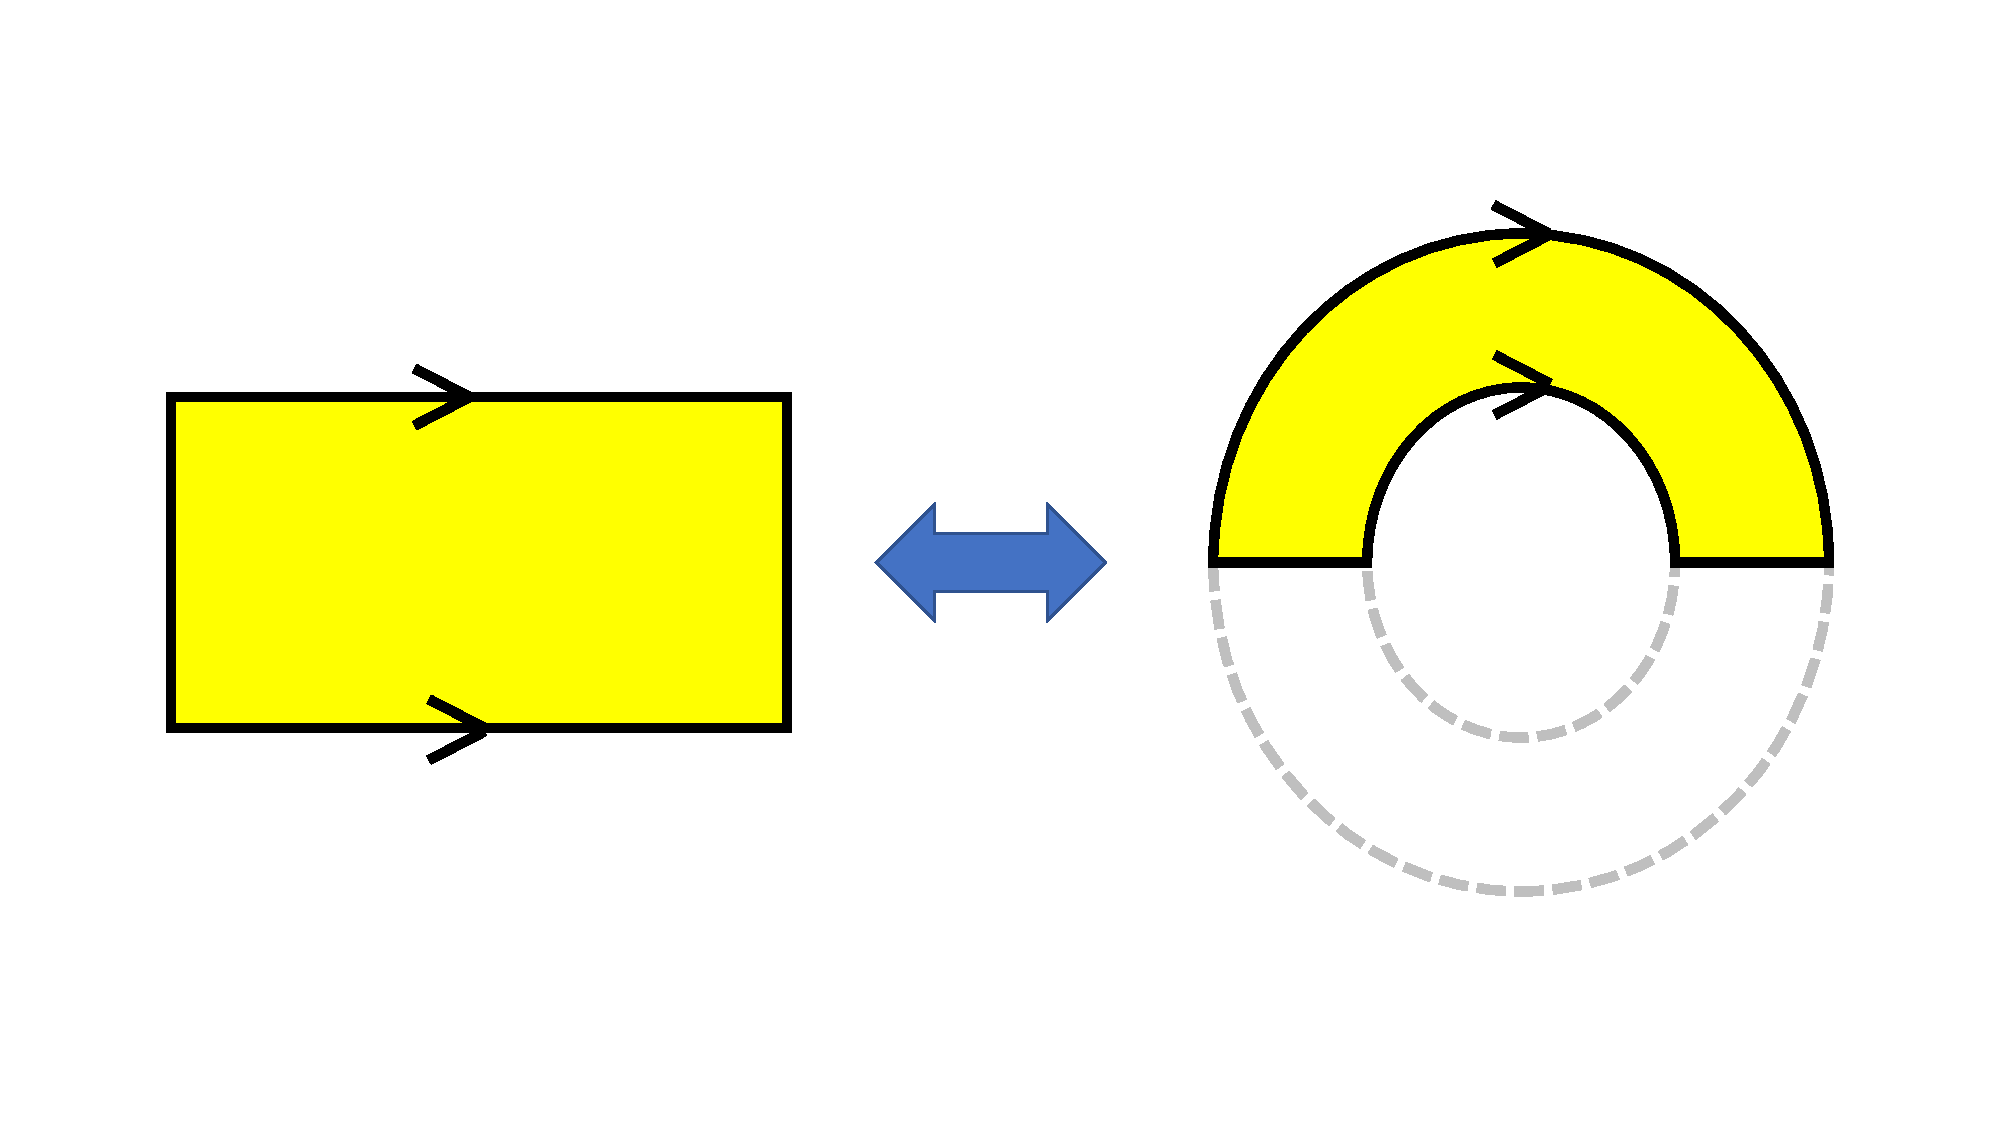
\includegraphics[width=0.7\linewidth]{cyl2uhp.pdf}
	\caption{左図は$w=x+i\tau,\  w\sim w+2\pi i\beta,\  -\pi/2\leq x \leq \pi/2$の円筒を表し、矢印の向きに沿って同一視されている。これを$z=ie^{-iw}$によって共形変換すると、右図のように上半平面上のバウムクーヘン型の領域に移る。}
	\label{fig:cyl2uhp}
\end{figure}

したがって上の設定での円筒分配関数は、$Z_\text{NS-NS}(i\beta)$を$1/2$乗すればよく、
\begin{align}
Z_{[-\pi/2,\pi/2]\times S_\beta^1,\text{NN,NS}}(i\beta)= \frac{\theta_3(0|i\beta)}{\eta(i\beta)}\label{diracPFfincyl}
\end{align}
となる。


\section{3次元反de Sitter時空(AdS$_3$)}\label{sec:ads3}
ここでは3次元の真空のEinstein方程式の負の宇宙定数を持つ解であり、無限遠方でVirasoro対称性を実現する漸近的AdS$_3$時空について論じる。3次元Einstein-Hilbert作用はChern-Simons作用になっており、時空の内部には物理的自由度は無い。しかし時空の``境界''にはVirasoro対称性をもった物理的自由度(``boundary graviton'')が存在できる。この事実はAdS$_3$/CFT$_2$対応において本質的に重要な役割を果たす。

\subsection{3次元重力理論とChern-Simons作用}
\subsub{Einstein方程式}
$3=1+2$次元重力理論を考える。Einstein-Hilbert作用は
\begin{oframed}
\begin{align}
S[g]=\frac{1}{16\pi G}\int_{(M,g)}d^3 x \sqrt{-\det{g}}(R-2\Lambda)
\end{align}
\end{oframed}
であり、真空のEinstein方程式は
\begin{align}
R_{\mu\nu}-\frac{1}{2}g_{\mu\nu}R+\Lambda g_{\mu\nu}=0
\end{align}
である。

3次元でWeylテンソルは消えるので、Einstein方程式の真空解となる$g_{\mu\nu}$は
\begin{align}
R_{\mu\nu\rho\sigma}=\Lambda(g_{\mu\rho}g_{\sigma\nu}-g_{\mu\sigma}g_{\rho\nu})
\end{align}
を満たす。これは断面曲率が$\Lambda$の定曲率空間に他ならない。

連結かつ単連結かつ測地的完備な定曲率Lorentz多様体は、$\Lambda=0$ならMinkowski空間に、$\Lambda>0$ならde Sitter(dS)空間に、$\Lambda<0$なら反de Sitter(anti de Sitter, AdS)空間に等長同型である。また、$d=3$においてそれぞれに作用する等長変換群は、MinkowskiがPoincare群$ISO(2,1)$、de Sitterが$SO(3,1)$、反de Sitterが$SO(2,2)$である。

\subsub{Einstein-Hilbert作用の書き換え}
境界のない向き付け可能擬Riemann多様体$M$の(局所的な開集合をとって)各点で正規直交基底をなすようなベクトル場の組${e_a^\mu(x)}$をとる。${e_a^\mu(x)}$は多脚場(vielbein)などと呼ばれる。
\begin{align}
g_{\mu\nu}e_a^\mu(x)e_b^\nu(x)=\eta_{ab}
\end{align}
計量$g$を使ってベクトル場と$1$形式を同一視して、$e_\mu^a=g_{\mu\nu}e_a^\nu$を定義する。定義から明らかに$e_\mu^a e_b^\mu=\delta_b^a,\ e_a^\mu e_\nu^a=\delta_\nu^\mu$が成り立つ。

$e=\det(e_\mu^a)=\sqrt{-\det g}$とすれば、反対称テンソルは$\epsilon_{\mu_1\cdots \mu_d}=e^{-1}\epsilon_{a_1\cdots a_d}e_{\mu_1}^{a_1} \cdots e_{\mu_d}^{a_d}$と書ける。

$M$の接束上のLevi-Civita接続を考えて、これを主$SO(p,q)$枠束に還元した$so(p,q)$値$1$形式を$\omega_\mu^{ab}$と書くと、$\omega$の曲率は
\begin{align}
R_{\mu\nu}^{ab}[\omega]&=(d\omega^{ab}+\omega^a_{\ c}\wedge\omega^{cb})_{\mu\nu}\notag\\
&=\del_\mu \omega_\nu^{ab}-\del_\nu \omega_\mu^{ab}+\omega_\mu^{ac}\omega_{\nu\ c}^{\ b}-\omega_\nu^{ac}\omega_{\mu\ c}^{\ b}
\end{align}
となる。これはLevi-Civita接続の曲率と$R_{\ \ \mu\nu}^{\rho\sigma}=e_a^\rho e_b^\sigma R_{\mu\nu}^{ab}$と関係している。

このとき$d$次元でのEinstein-Hilbert作用$S[g]=\frac{1}{16\pi G}\int_{(M,g)}d^d x \sqrt{-\det{g}}(R-2\Lambda)$は次のように書き換えられる。
\begin{align}
S[g]=\frac{1}{16\pi G}\int_{(M,g)} \epsilon_{a_1\cdots a_d}(e^{a_1}\wedge\cdots\wedge e^{a_{d-2}}\wedge R^{a_{d-1}a_d}[\omega]-\frac{2\Lambda}{d!}e^{a_1}\wedge\cdots\wedge e^{a_d})
\end{align}

とくに$d=3$なら、
\begin{align}
S[g]=\frac{1}{2\pi}\int_{(M,g)} \epsilon_{abc}(e^{a}\wedge R^{bc}[\omega]-\frac{\Lambda}{3}e^a\wedge e^b\wedge e^c)
\end{align}
である。さらに$\omega^{ab},R^{ab}$のHodge双対を
\begin{align}
\omega_a=\frac{1}{2}\epsilon_{abc}\omega^{bc},\ R_a=\frac{1}{2}\epsilon_{abc}R^{bc}=d\omega^a+\frac{1}{2}\epsilon_{abc}\omega^b\wedge \omega^c
\end{align}
で定義すると、これらは$so(p,q)\ (p+q=3)$ベクトル値$1$形式になっている。

これを用いて3次元Einstein-Hilbert作用を
\begin{align}
S[g]=\frac{1}{16\pi G}\int_{(M,g)} (e^{a}\wedge R_a[\omega]-\frac{\Lambda}{3}\epsilon_{abc} e^a\wedge e^b\wedge e^c)
\end{align}
と書くことができる。

\subsub{Chern-Simons作用}
以下では$\Lambda<0$のときにEinstein-Hilbert作用がChern-Simons作用として書けることを見る。

$SO(2,2)$のLie代数は$so(2,2)\simeq sl(2,\R)\directsum sl(2,\R)$と分解でき、各$sl(2,\R)$の生成子$J_a^\pm$を次を満たすようにとることができる。
\begin{align}
[J_a^+,J_b^+]=\epsilon_{abc}J^{c+},&&[J_a^-,J_b^-]=\epsilon_{abc}J^{c-},&&[J_a^+,J_b^-]=0\\
\Tr J_a^+ J_b^+=\frac{1}{2}\eta_{ab},&&\Tr J_a^- J_b^-=\frac{1}{2}\eta_{ab},&&\Tr J_a^+ J_b^-=0
\end{align}


このとき各$SL(2,\R)$ゲージ場を
\begin{align}
A_\mu\coloneqq \left(\omega_\mu^a-\sqrt{-\Lambda}e_\mu^a\right) J_a^-,\ \overline{A}_\mu\coloneqq \left(\omega_\mu^a+\sqrt{-\Lambda}e_\mu^a\right) J_a^+
\end{align}
で定義すると、$\del M=\emptyset$より、Einstein-Hilbert作用はそれぞれの$SL(2,\R)$ゲージ場のChern-Simons作用の和として書ける。
\begin{oframed}
\begin{align}
S[g]&=S_{CS}[A]-S_{CS}[\overline{A}]\\
S_{CS}[A]&=\frac{k}{4\pi}\int_M \Tr \left( A\wedge dA+\frac{2}{3}A\wedge A\wedge A \right)\\
k&=-\frac{1}{4G\sqrt{-\Lambda}}
\end{align}
\end{oframed}

したがって3次元Einstein-Hilbert作用は多様体の大域的なトポロジーにしか依らず、内部には自由度が存在しない。これは3次元ではWeylテンソルが消えて重力波が存在しないこととも捉えられる。

しかし多様体の境界には自由度が存在することができて、この自由度による計量のダイナミクスは\textbf{boundary graviton}と呼ばれる。

\subsection{漸近的AdS$_3$時空}
\subsub{global AdS計量とPoincare計量}
\begin{oframed}
$\R^{2,2}$の座標を$X^0,X^1,X^2,X^3$とし、計量を$ds^2=-(dX^0)^2-(dX^1)^2+(dX^2)^2+(dX^3)^2$とする。\textbf{AdS$_3$時空}を$\R^{2,2}$内の$3$次元部分多様体
\begin{align}
-(X^0)^2-(X^1)^2+(X^2)^2+(X^3)^2=-R_A^2
\end{align}
として定義する。
\end{oframed}

部分多様体全体を覆う座標$(t,\rho_\text{emb},\varphi)$として
\begin{align}
X^0&=R_A \cosh\rho_\text{emb} \cos t\\
X^1&=R_A \cosh\rho_\text{emb} \sin t\\
X^2&=R_A \sinh\rho_\text{emb} \cos \varphi\\
X^3&=R_A \sinh\rho_\text{emb} \sin \varphi
\end{align}
が取れる。ただし$t\sim t+2\pi,\  \varphi\sim \varphi+2\pi$の周期性を持つので、時間的閉曲線が出ないように$t$方向に$\R\to S^1$の被覆をとる。このとき部分多様体上の誘導計量は
\begin{align}
ds^2=R_A^2 (-\cosh^2 \rho_\text{emb} dt^2+d\rho_\text{emb}^2+\sinh^2\rho_\text{emb}d\varphi^2)
\end{align}
となる。また、$r_{B}=R_A\sinh\rho_\text{emb}$と動径方向を変数変換すれば計量は
\begin{oframed}
\begin{align}\label{globalAdS}
ds^2=-R_A^2\left(1+\frac{r_{B}^2}{R_A^2}\right)dt^2+\left(1+\frac{r_{B}^2}{R_A^2}\right)^{-1}dr_{B}^2+r_{B}^2d\varphi^2
\end{align}
\end{oframed}

となる。この計量は\textbf{global AdS$_3$}計量やpure AdS$_3$計量と呼ばれ、$\Lambda=-1/R_A ^2<0$のEinstein方程式の真空解になっている。$R_A$は宇宙定数の平方根であるが、$\R^{2,2}$への埋め込みの大きさを決めるパラメータでもあり、$R_A$は\textbf{AdS半径}と呼ばれる。global AdS$_3$は図\ref{fig:globalads}のように、円筒として描かれる。
\begin{figure}[h]
	\centering
	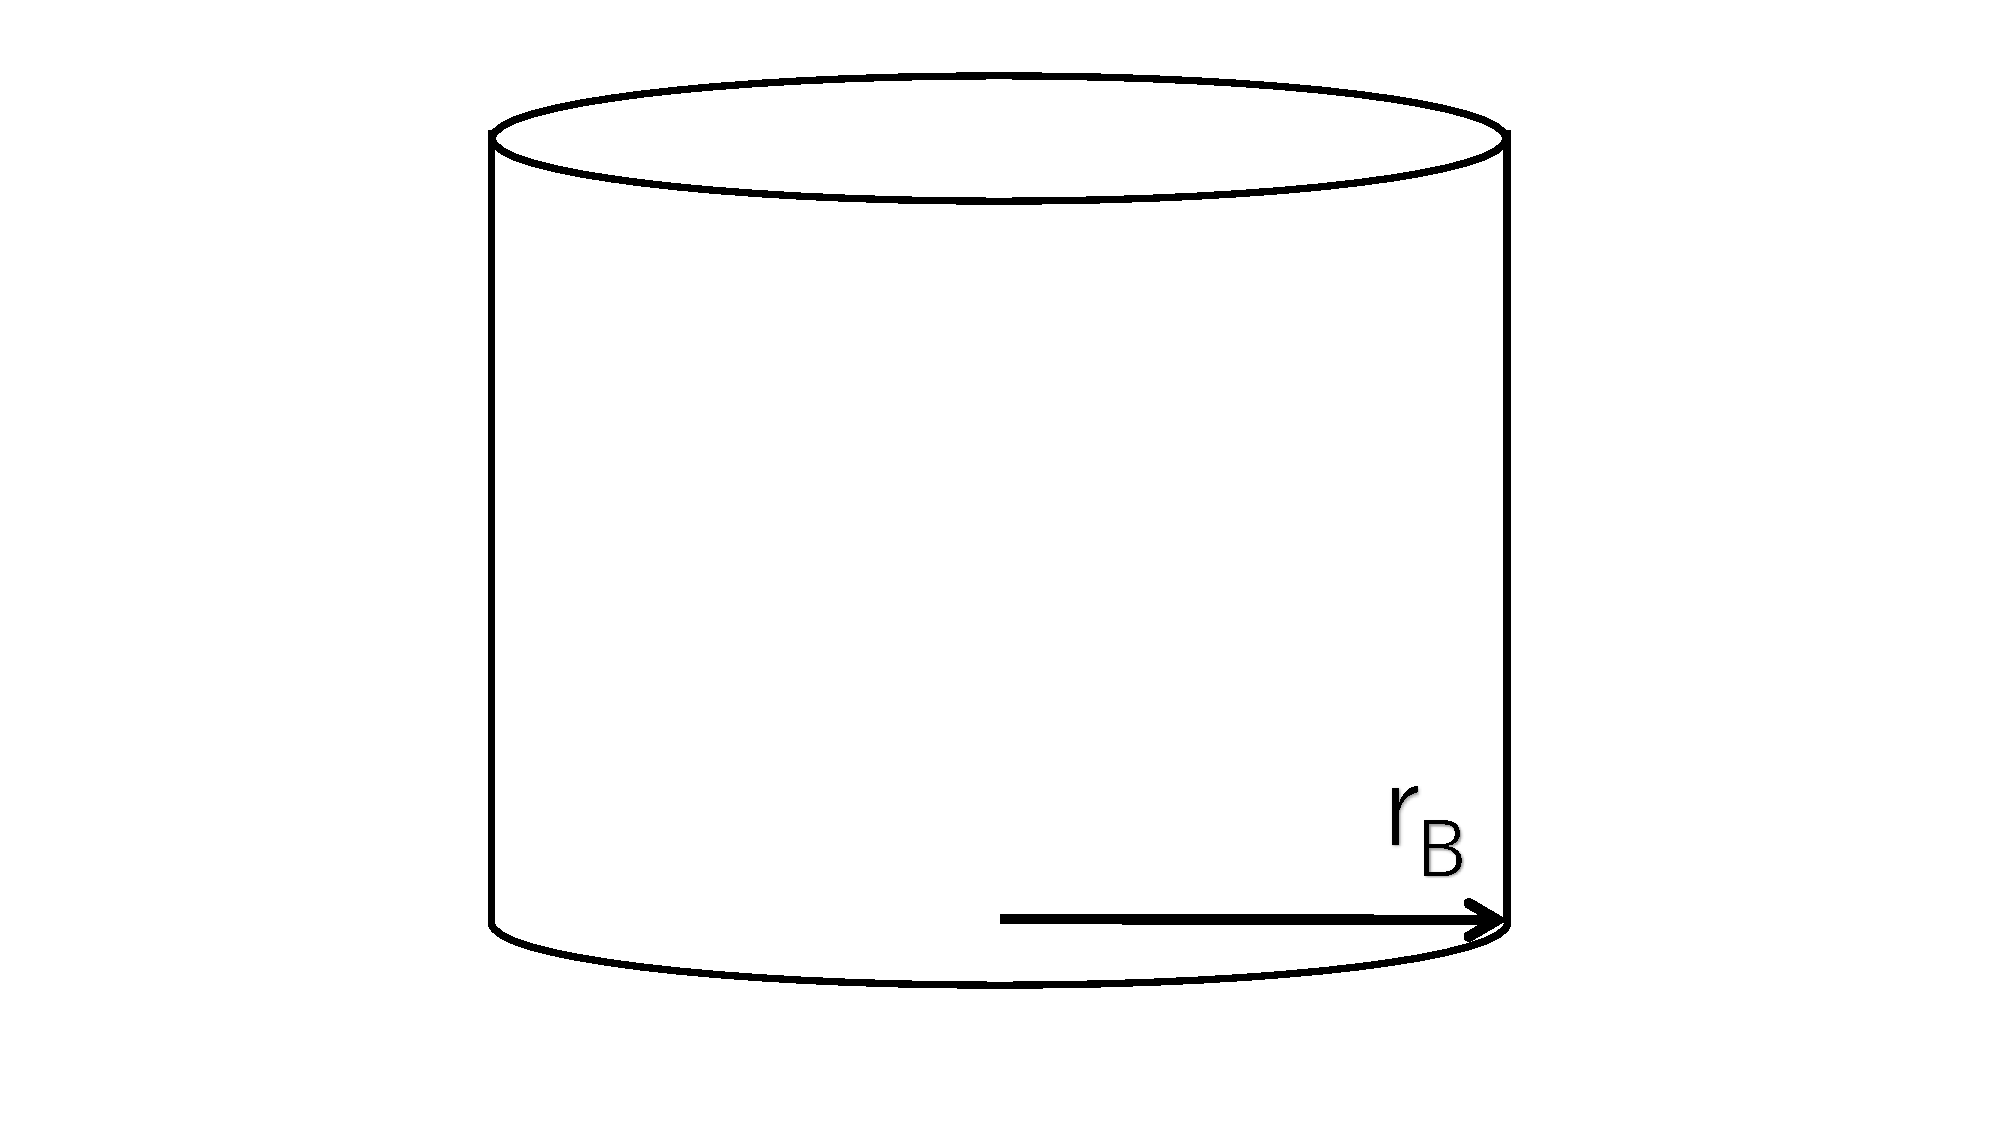
\includegraphics[width=0.7\linewidth]{globalAdS.pdf}
	\caption{global AdS$_3$の図。円の動径方向が$r$軸に対応している。}
	\label{fig:globalads}
\end{figure}

部分多様体の一部を覆う局所座標$(t_P,x_P,z_P),\ (z_P>0)$を
\begin{align}
X^0&=\frac{z_P}{2}\left( 1+\frac{R_A^2-t_P^2+x_P^2}{z_P^2} \right)\\
X^1&=\frac{R_A t_P}{z_P}\\
X^2&=\frac{z_P}{2}\left( 1+\frac{-R_A^2-t_P^2+x_P^2}{z_P^2} \right)\\
X^3&=\frac{R_A x_P}{z_P}
\end{align}
で定義すると、計量は
\begin{oframed}
\begin{align}\label{Poincaremetric}
ds^2=R_A^2\frac{-dt_P^2+dx_P^2+dz_P^2}{z_P^2}
\end{align}
\end{oframed}
となる。これは\textbf{Poincare計量}と呼ばれる。$r_P=1/z_P$と変数変換すれば
\begin{align}\label{Poincarer}
ds^2=R_A^2\left(\frac{dr_P^2}{r_P^2}+r_P^2(-dt_P^2+dx_P^2)\right)
\end{align}
となる。global AdS$_3$は図\ref{fig:poincare}のように描かれる。
\begin{figure}[h]
	\centering
	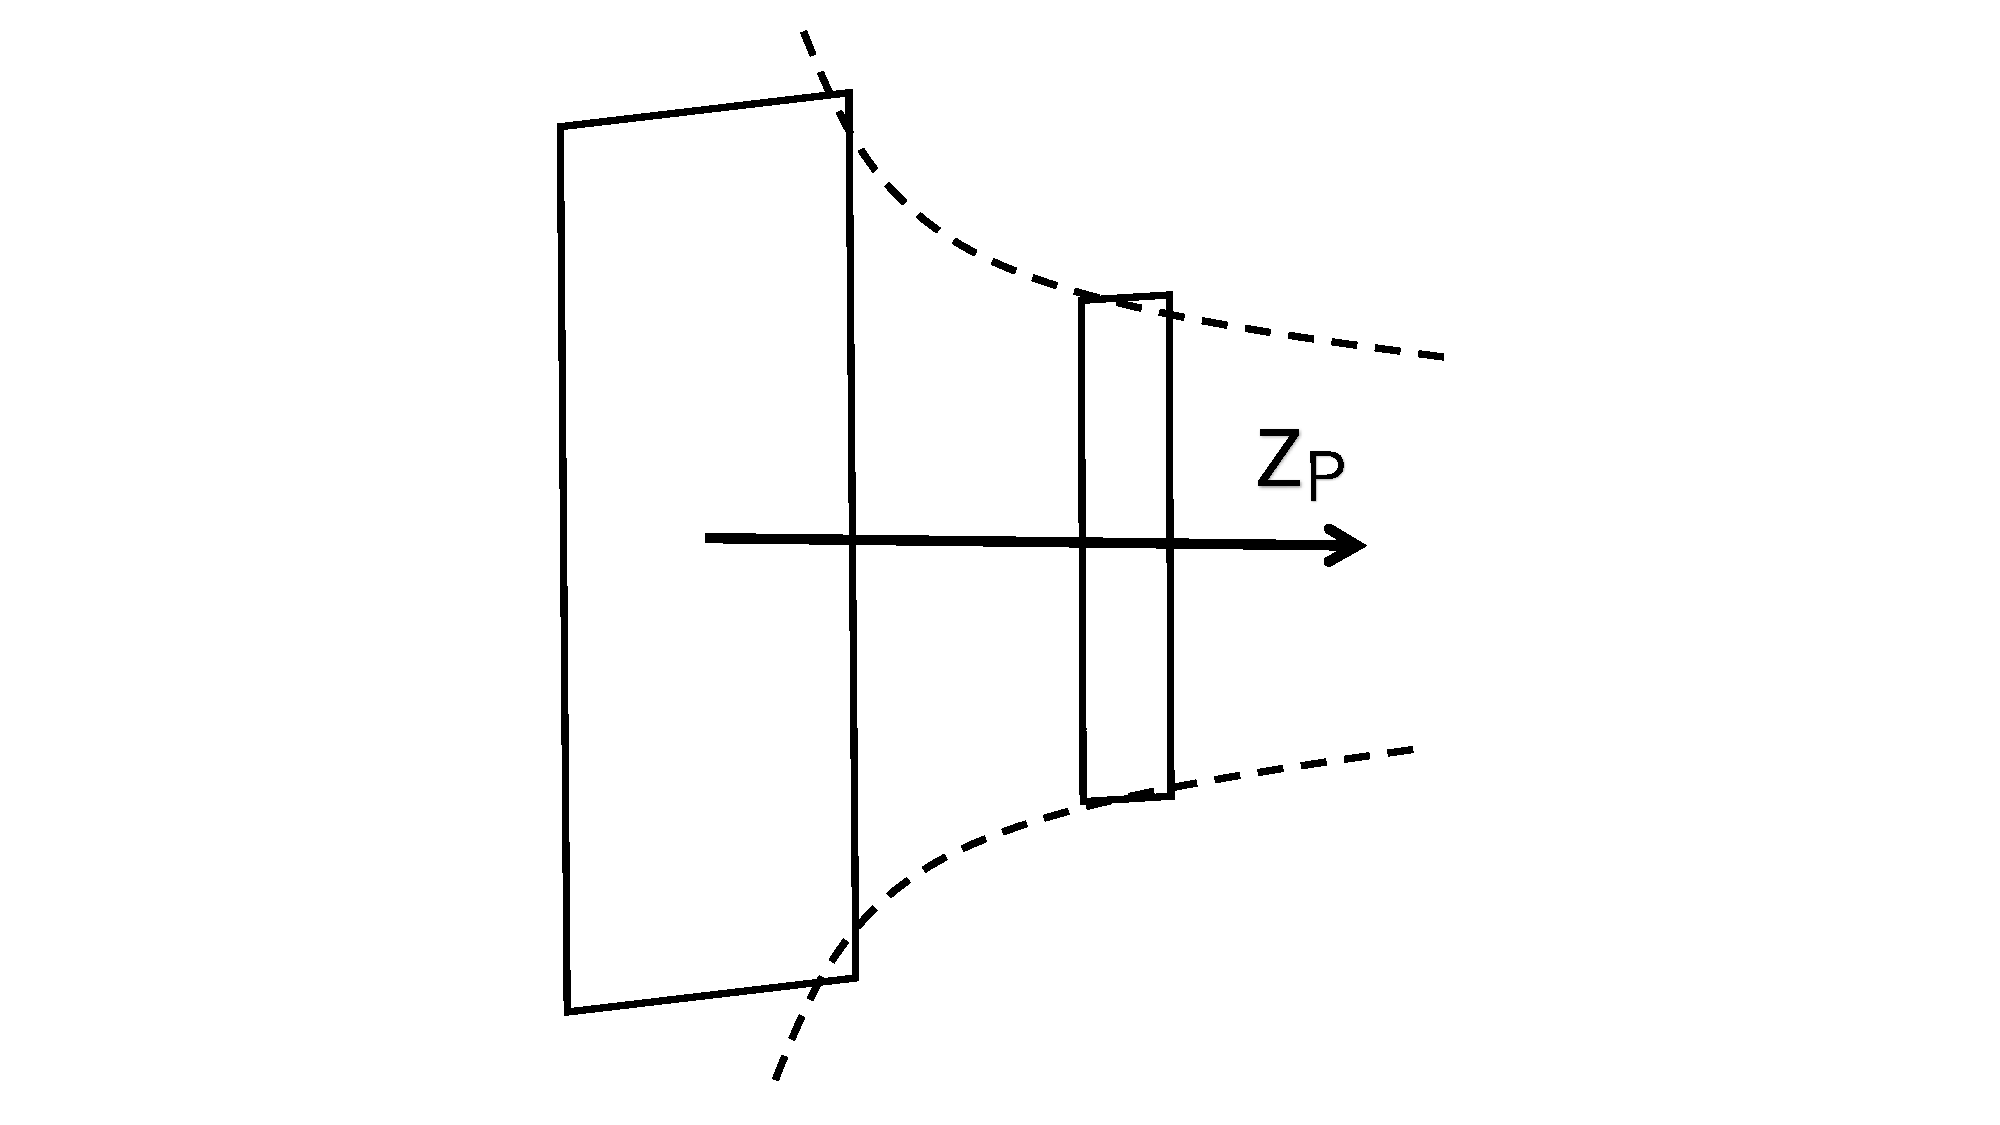
\includegraphics[width=0.7\linewidth]{Poincare.pdf}
	\caption{Poincare座標の図。$z_P$が大きくなるにつれて計量の$\det$が小さくなっていく。}
	\label{fig:poincare}
\end{figure}

\subsub{漸近的AdS$_3$時空の定義}
\begin{oframed}
以下では円筒座標$(t,r,\varphi),\ \varphi\sim \varphi+2\pi$を取り、$r=(\text{一定})$の面上の光円錐座標を$x^\pm=\varphi\pm t,\ \del_{\pm}=\frac{1}{2}(\del_\varphi\pm \del_t)$で定義しておく。このとき、次の形を満たす計量を考える。
\begin{align}
&&ds^2&=R_A^2\left(\frac{dr^2}{r^2}+\gamma_{ij}(r,x^+,x^-)dx^i dx^j\right)&&(i,j=\pm)\\
&&\gamma_{ij}dx^i dx^j&=r^2dx^- dx^+ +O(1)_{ij}dx^i dx^j&&(r\to\infty)
\end{align}
上の$r\to\infty$での境界条件を\textbf{Brown-Henneaux境界条件}\cite{Brown:1986nw}という。また、$r\to\infty$でこの計量はPoincare計量(\ref{Poincarer})に一致する。それゆえこの計量で表される時空は\textbf{漸近的AdS$_3$(asymptotic AdS)時空}と呼ばれる。

$\Lambda=-1/R_A ^2<0$のEinstein方程式の解となる漸近的AdS$_3$時空の計量は次の形に限られる\cite{Banados:1998gg}ことが知られていて、\textbf{Fefferman-Graham計量}\cite{FeffermanGraham}と呼ばれる。
\begin{align}\label{Feffermangraham}
ds^2=R_A^2\left(\frac{dr^2}{r^2}+\left(rdx^+ +\frac{L(x^-)}{r}dx^- \right)\left(rdx^- +\frac{\overline{L}(x^+)}{r}dx^+ \right)\right)
\end{align}
ここで$L(x^-),\overline{L}(x^+)$はそれぞれ$x^-,x^+$のみの関数であることに注意しておく。
\end{oframed}

Poincare計量は$L=\overline{L}=0$のFefferman-Graham計量になっている。

\subsub{漸近的Virasoro対称性}
いま光円錐座標$(x^-,x^+,r)$での接空間のミンコフスキー計量を
\begin{align}
\eta=\left(\begin{array}{ccc}
0 & 1 & 0 \\
1 & 0 & 0 \\
0 & 0 & 1 \end{array}
\right)
\end{align}
と定める。これに対応する$sl(2,\R)$の生成子を
\begin{align}
j_-=\frac{1}{\sqrt{2}}\left(\begin{array}{cc}
0 & 1 \\
0 & 0\end{array}
\right),\ 
j_+=\frac{1}{\sqrt{2}}\left(\begin{array}{cc}
0 & 0 \\
1 & 0\end{array}
\right),\ 
j_r=\frac{1}{2}\left(\begin{array}{cc}
1 & 0 \\
0 & -1\end{array}
\right)
\end{align}
ととると、$[j_a,j_b]=\epsilon_{abc}j_c,\ \Tr(j_aj_b)=\frac{1}{2}\eta_{ab}$を満たしている。

このとき計量(\ref{Feffermangraham})に対する$e^a,\omega^a$は
\begin{align}
e^-&=R_A\left(\frac{r}{\sqrt{2}}dx^-+\frac{\overline{L}(x^+)}{\sqrt{2}r}dx^+\right),&
e^+&=R_A\left(\frac{r}{\sqrt{2}}dx^++\frac{L(x^-)}{\sqrt{2}r}dx^-\right),&
e^r&=R_A\frac{dr}{r}\\
\omega^-&=-\frac{r}{\sqrt{2}}dx^-+\frac{\overline{L}(x^+)}{\sqrt{2}r}dx^+,&
\omega^+&=\frac{r}{\sqrt{2}}dx^+-\frac{L(x^-)}{\sqrt{2}r}dx^-,&
\omega^r&=0
\end{align}
であり、対応する$SL(2,\R)$ゲージ場は
\begin{align}
A=\left(\begin{array}{cc}
-\frac{1}{2r}dr & -rdx^- \\
-\frac{L(x^-)}{r}dx^- & \frac{1}{2r}dr \end{array}
\right),\ 
\overline{A}=\left(\begin{array}{cc}
\frac{1}{2r}dr & \frac{\overline{L}(x^+)}{r}dx^+ \\
rdx^+ & -\frac{1}{2r}dr \end{array}
\right)
\end{align}
となる。ここで$A,\overline{A}$は$x^-,x^+$成分に分解していることに注意する。ここで$x^\pm$を混ぜない$SL(2,\R)$ゲージ固定
\begin{align}
a=b^{-1}Ab+b^{-1}db,\ \overline{a}=b\overline{A}b^{-1}+bd(b^{-1}),\ b=\left(\begin{array}{cc}
r^{1/2} & 0\\
0 & r^{-1/2} \end{array}
\right)
\end{align}
をすると$A,\overline{A}$の$r$依存性は消えて、それぞれ$x^-,x^+$のみの関数となる。
\begin{align}
a(x^-)=\left(\begin{array}{cc}
0 & -1 \\
-L(x^-) & 0 \end{array}
\right)dx^-,\ 
\overline{a}(x^+)=\left(\begin{array}{cc}
0 & \overline{L}(x^+) \\
1 & 0 \end{array}
\right)dx^+
\end{align}
$a,\overline{a}$は境界の座標$x^\pm$にしか依存しておらず、したがってこの自由度がboundary gravitonを表している。

いま$a,\overline{a}$の成分のうち、$L,\overline{L}$のみ変えるような無限小ゲージ変換$\delta a=\del_-\lambda+[a,\lambda],\delta \overline{a}=\del_+\overline{\lambda}+[\overline{a},\overline{\lambda}]$はそれぞれ$1$つの関数によって決まり、
\begin{align}
\lambda=\left(\begin{array}{cc}
\frac{1}{2}\del_-\epsilon & -\epsilon \\
-(L(x^-)-\frac{1}{2}\del_-^2)\epsilon & -\frac{1}{2}\del_-\epsilon \end{array}
\right),\quad
\overline{\lambda}=\left(\begin{array}{cc}
-\frac{1}{2}\del_+\overline{\epsilon} & (\overline{L}(x^+)-\frac{1}{2}\del_+^2)\overline{\epsilon} \\
\overline{\epsilon} & \frac{1}{2}\del_+\overline{\epsilon}
\end{array}
\right)
\end{align}
で与えられる。ただし$\epsilon,\overline{\epsilon}$はそれぞれ$x^-,x^+$のみの関数である。これにより$L,\overline{L}$は
\begin{align}\label{infinitestimaltransfofL}
\delta L&=\epsilon \del_- L +2L\del_- \epsilon -\frac{1}{2}\del_-^3\epsilon\\
\delta \overline{L}&=\overline{\epsilon} \del_+ \overline{L} +2\overline{L}\del_+ \overline{\epsilon} -\frac{1}{2}\del_+^3\overline{\epsilon}
\end{align}
と変換する。このゲージ対称性は、boundary gravitonのもつ対称性を表している。

ここで$T=-kL,\overline{T}=-k\overline{L}$として
\begin{align}
L_m&\coloneqq -\frac{1}{2\pi}\int_{0}^{2\pi} e^{im\varphi}T d\varphi\\
\overline{L}_m&\coloneqq -\frac{1}{2\pi}\int_{0}^{2\pi} e^{im\varphi}\overline{T} d\varphi
\end{align}
とモード展開すると、$L_m,\overline{L}_m$は$SL(2,\R)$ゲージ固定をして得られるDirac括弧$\{\ ,\ \}$の交換関係
\begin{align}
i\{L_m,L_n\}&=(m-n)L_{m+n}-\frac{k}{2}m^3\delta_{m+n,0}\\
i\{L_m,\overline{L}_n\}&=0\\
i\{\overline{L}_m,\overline{L}_n\}&=(m-n)\overline{L}_{m+n}-\frac{k}{2}m^3\delta_{m+n,0}
\end{align}
を満たす。


したがって、$L_m-\frac{k}{4}\delta_{m,0},\overline{L}_n-\frac{k}{4}\delta_{n,0}$は中心電荷
\begin{oframed}
\begin{align}
c_A=-6k=\frac{3R_A}{2G}
\end{align}
\end{oframed}
のVirasoro代数の生成子になっており、$c_A$はBrown-Henneaux中心電荷\cite{Brown:1986nw}と呼ばれることも多い。いま$L_m-\frac{k}{4}\delta_{m,0},\overline{L}_n-\frac{k}{4}\delta_{n,0}$が古典Virasoro代数の生成子になったが、このことは円筒上のCFT$_2$を平面に共形変換するとエネルギー運動量テンソルが$T_\text{円筒}=T_\text{平面}+c/24$と中心電荷のぶんだけずれることに似ている。

3次元AdS重力には内部には自由度はないが、境界にはboundary gravitonの自由度を持つことができ、それはFefferman-Graham計量の$L,\overline{L}$によって記述される。さらにboundary gravitonの自由度もゲージ対称性を持ち、$L_m-\frac{k}{4}\delta_{m,0},\overline{L}_n-\frac{k}{4}\delta_{n,0}$がVirasoro代数の生成子となるのである。

\subsection{様々な漸近的AdS$_3$計量}
\subsub{BTZ計量}
$T,\overline{T}$を用いてFefferman-Graham計量(\ref{Feffermangraham})は
\begin{align}\label{FeffermangrahamT}
ds^2&=R_A^2\left(\frac{dr^2}{r^2}+\left(rdx^+ +\frac{4G}{R_A r}T(x^-)dx^- \right)\left(rdx^- +\frac{4G}{R_A r}\overline{T}(x^+)dx^+ \right)\right) \notag\\
&=\frac{R_A^2}{r^2}dr^2+4GR_A Tdx^{-2}+4GR_A \overline{T}dx^{+2}+\left(R_A^2 r^2+\frac{16G^2}{r^2}T\overline{T}\right)dx^-dx^+
\end{align}
と書ける。

$r=1/z$と変数変換すれば、
\begin{align}\label{FeffermangrahamZ}
ds^2=\frac{R_A ^2}{z^2}dz^2+4GR_A Tdx^{-2}+4GR_A \overline{T}dx^{+2}+\left(\frac{R_A^2}{z^2}+16G^2 z^2 T(x^-)\overline{T}\right)dx^-dx^+
\end{align}
となる。また$r=e^\rho$と変数変換すれば、
\begin{align}\label{FeffermangrahamRHO}
ds^2&=R_A^2 d\rho^2+4GR_A Tdx^{-2}+4GR_A \overline{T}dx^{+2}+\left(R_A^2 e^{2\rho}+16G^2 e^{-2\rho}T\overline{T}\right)dx^-dx^+
\end{align}
となる。さらに、$T,\overline{T}$が定数のとき
\begin{oframed}
\begin{align}
T+\overline{T}&=MR_A=\frac{r_+^2+r_-^2}{8GR_A}\\
T-\overline{T}&=J=\frac{2r_+r_-}{8GR_A}\\
r_\pm^2&=4GR_A^2M \left(1\pm\sqrt{1-(J/MR_A)^2}\right)
\end{align}
\end{oframed}
で$r_\pm,M,J$を定義して、動径方向を
\begin{align}
r_{B}^2&=r_+^2\cosh^2(\rho-\rho_0)-r_-^2\sinh^2(\rho-\rho_0)\\
e^{2\rho_0}&=(r_+^2-r_-^2)/(4R_A^2)
\end{align}
と変数変換すれば、
\begin{oframed}
\begin{align}\label{FeffermangrahamBTZ}
ds^2&=-R_A^2(N(r_{B}))^2dt^2+(N(r_{B}))^{-2}dr_{B}^2+r_{B}^2(d\varphi+N^\varphi(r)dt)^2\\
&=-\frac{(r_{B}^2-r_+^2)(r_{B}^2-r_-^2)}{r_{B}^2}dt^2+\frac{r_{B}^2R_A^2}{(r_{B}^2-r_+^2)(r_{B}^2-r_-^2)}dr_{B}^2+r_{B}^2\left(d\varphi-\frac{r_+r_-}{r_{B}^2R_A}dt\right)^2\\
(N(r_{B}))^2&=-8MG+\frac{r_{B}^2}{R_A^2}+\frac{16G^2J^2}{r_{B}^2}=\frac{(r_{B}^2-r_+^2)(r_{B}^2-r_-^2)}{r_{B}^2R_A^2}\\
N^\varphi(r_{B})&=-\frac{4GJ}{r_{B}^2}=-\frac{r_+r_-}{r_{B}^2R_A}
\end{align}
\end{oframed}
となる。これはAdS$_3$時空でのKerrブラックホールを記述する計量で、\textbf{BTZ(Banados-Teitelboim-Zanelli)計量}\cite{Banados:1992wn}と呼ばれる。

$|J|\leq MR_A$のとき、$M,J$はブラックホールのADM質量、角運動量に対応し、$r_+,r_-$はイベントホライズン、Cauchyホライズンに対応する。とくに$|J|=MR_A\iff r_+=r_-$のときのブラックホールは\textbf{極限(extremal) BTZブラックホール}と呼ばれる。$|J|< MR_A$のときは非極限(non-extremal) BTZブラックホールと呼ばれる。

\begin{oframed}
$J=0\iff r_-=0$のときの計量は
\begin{align}
ds^2=-(r_{B}^2-r_+^2)dt^2+\frac{R_A^2}{r_{B}^2-r_+^2}dr_{B}^2+r_{B}^2d\varphi^2
\end{align}
であり、さらに$z_{B}=R_A/r_{B},z_+=R_A/r_+$と変数変換すれば、
\begin{align}\label{BTZblackbrane}
ds^2=\frac{R_A^2}{z_{B}^2}\left( -\left(1-\frac{z_{B}^2}{z_+^2}\right)dt^2+\left(1-\frac{z_{B}^2}{z_+^2}\right)^{-1}dz_{B}^2+d\varphi^2 \right)
\end{align}
となる。この計量は\textbf{non-rotating BTZ計量}やAdS$_3$ Schwartzschild計量、あるいはAdS$_3$ black brane計量などと呼ばれる。
\end{oframed}
non-rotating BTZ時空は図\ref{fig:btz}のように、global AdSに穴が開いたような構造をしている。
\begin{figure}[h]
	\centering
	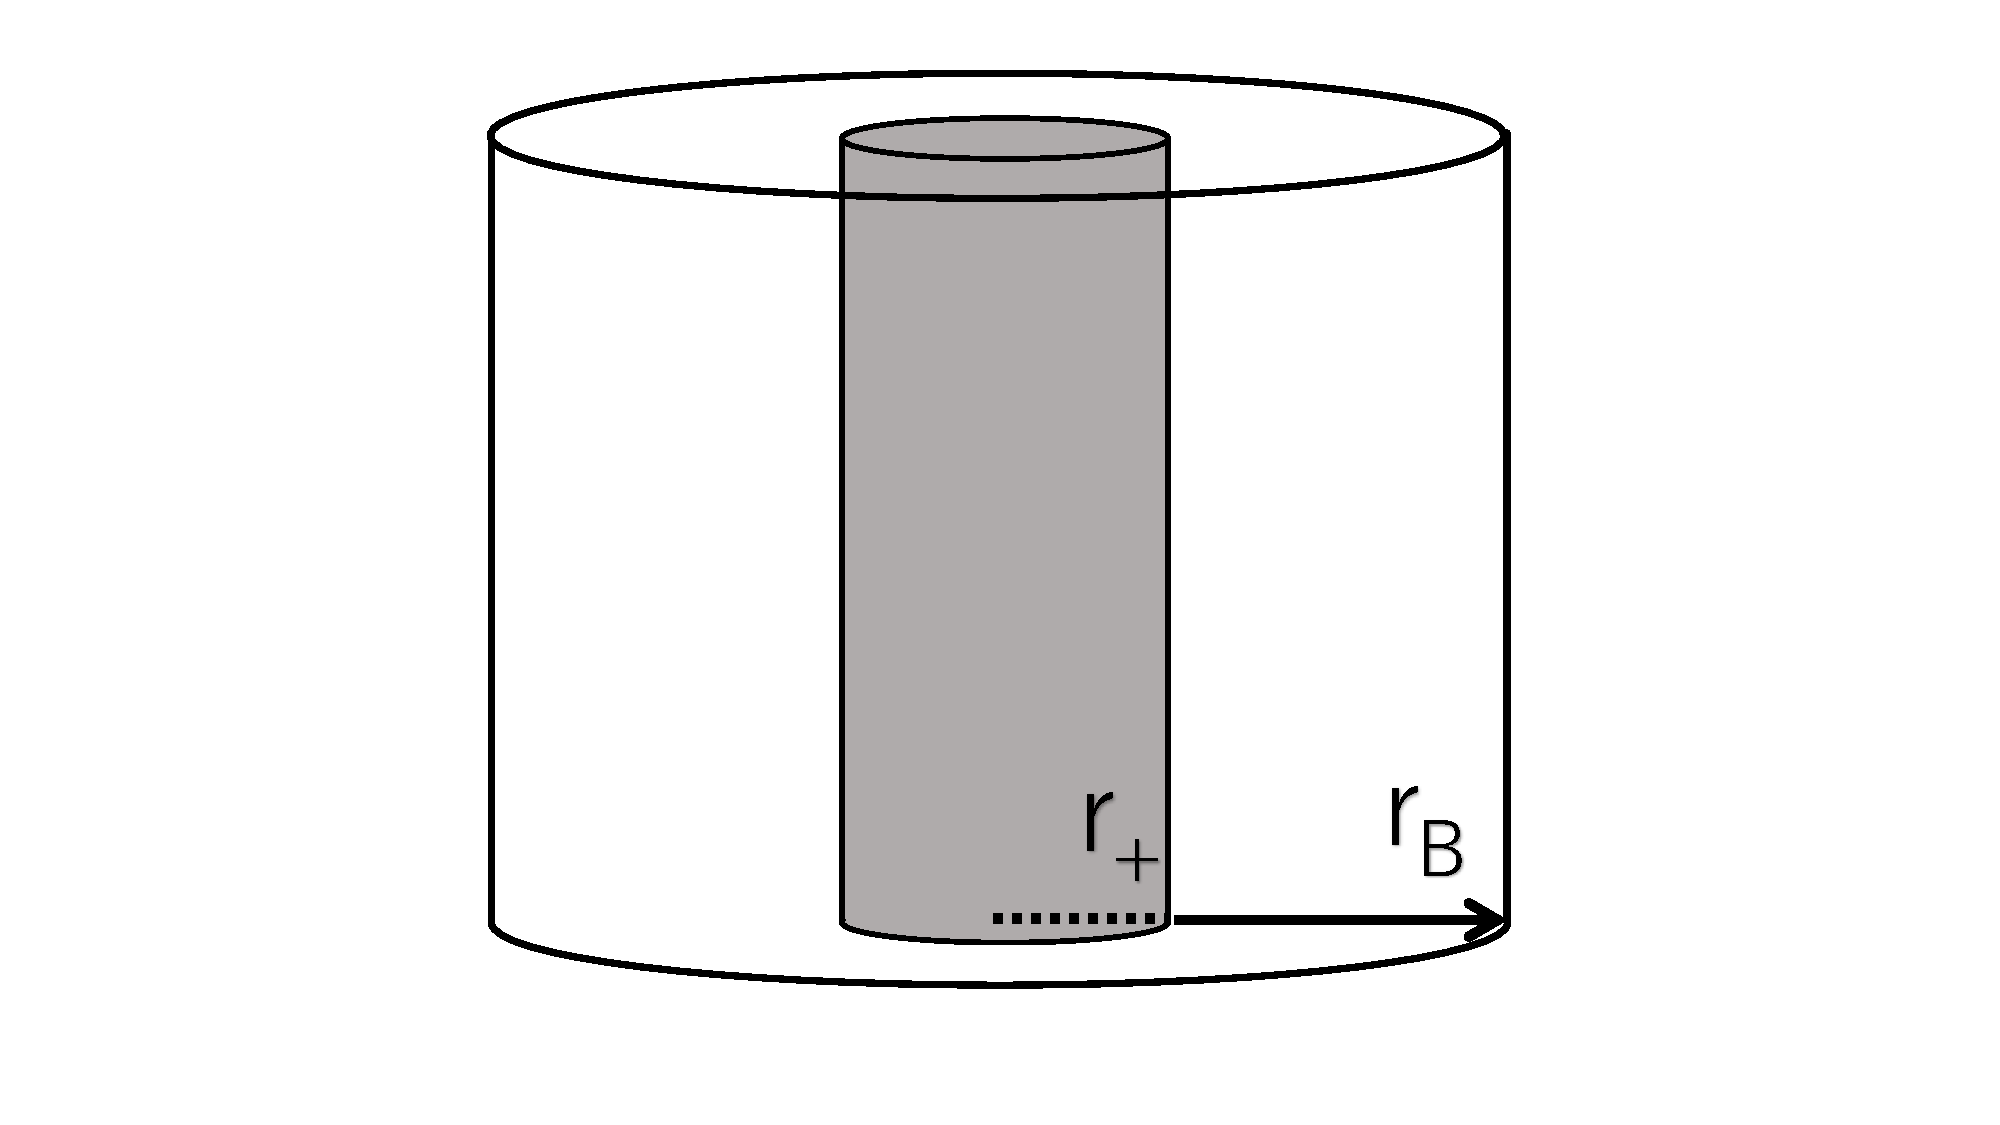
\includegraphics[width=0.7\linewidth]{BTZ.pdf}
	\caption{non-rotating BTZ時空の図。灰色の部分はホライズンの内側を表していて、そこでは計量は定義されていない。}
	\label{fig:btz}
\end{figure}

特に$r_+=r_-=0$の計量
\begin{align}\label{BPSBTZ}
ds^2=\frac{R_A^2}{r_{B}^2}dr_{B}^2+r_{B}^2(-dt^2+d\varphi^2)
\end{align}
は零質量BTZ (massless BTZ)ブラックホールや\textbf{BPS(Bogomol'nyi–Prasad–Sommerfield) BTZブラックホール}と呼ばれる。これは極限BTZブラックホールになっている。

\subsub{global AdS計量とPoincare計量}
$M=-1/(8G),J=0$のときのBTZ計量はホライズン$r_\pm$を持たず、global AdS$_3$計量
\begin{align}
ds^2=-R_A^2\left(1+\frac{r_{B}^2}{R_A^2}\right)dt^2+\left(1+\frac{r_{B}^2}{R_A^2}\right)^{-1}dr_{B}^2+r_{B}^2d\varphi^2
\end{align}
になる。

任意の漸近的AdS$_3$計量は局所的にはPoincare計量にゲージ同値である。したがってPoincare計量(\ref{Poincaremetric})とFefferman-Graham計量(\ref{FeffermangrahamZ})は変数変換で移りあえるが、実際これを実現する変数変換が知られており\cite{Roberts_2012}、以下で紹介する。

Poincare計量
\begin{align}
ds^2=R_A^2\frac{dz_P^2+dx_P^-dx_P^+}{z_P^2}
\end{align}
に対して、$x^-,x^+$のみの関数$f(x^-),\overline{f}(x^+)$をとり、
\begin{oframed}
\begin{align}
x_P^-&=f(x^-)-\frac{2z^2(f')^2\overline{f}''}{4f'\overline{f}'+z^2f''\overline{f}''}\label{robertsmap1}\\
x_P^+&=\overline{f}(x^+)-\frac{2z^2(\overline{f}')^2f''}{4f'\overline{f}'+z^2f''\overline{f}''}\label{robertsmap2}\\
z_P&=\frac{4z(f'\overline{f}')^{3/2}}{4f'\overline{f}'+z^2f''\overline{f}''}\label{robertsmapz}
\end{align}
\end{oframed}
として座標変換$(x^\pm,z)\to (x_P^\pm,z_P)$を定義すると、Fefferman-Graham計量(\ref{FeffermangrahamZ})において
\begin{align}
\frac{4G}{R_A} T(x'^-)=\frac{3(f'')^2-2f'f'''}{4f'^2},\ \frac{4G}{R_A} \overline{T}(x'^+)=\frac{3(\overline{f}'')^2-2\overline{f}'\overline{f}'''}{4\overline{f}'^2}
\end{align}
としたものに変換される。$T,\overline{T}$の変換は無限小変換(\ref{infinitestimaltransfofL})を有限変換にしたものに他ならない。いま$c_A=-3R_A/2G$を用いて表せば、
\begin{align}
T(x'^-)&=\frac{c_A}{12}\{f(x'^-),x'^-\}\\
T(x'^+)&=\frac{c_A}{12}\{f(x'^+),x'^+\}
\end{align}
と表すことができる。

Poincare座標は$T=\overline{T}=0$のFefferman-Graham計量であり、$z\downarrow 0$での座標変換$(x'^\pm,z)\to (x_P^\pm,z_P)$は$x_P^-\to f(x'^-),x_P^+\to \overline{f}(x'^+)$であるから、上の$T,\overline{T}$の変換性は$z\downarrow 0$に存在する共形場理論のエネルギー運動量テンソルの共形変換$f$に対する変換性(\ref{transfofEmtensor})に一致している。

\subsection{有限温度の計量とHawking-Page相転移}
\subsub{有限温度の計量}
global AdS$_3$ (\ref{globalAdS})の時間をユークリッド化$\tau=it$して、$\tau\sim \tau+2\pi \beta_A/R_A$の周期境界条件をつけて有限温度化したものを\textbf{thermal AdS$_3$}と呼ぶ。
\begin{align}\label{tads}
ds^2&=R_A^2\left(1+\frac{r_{B}^2}{R_A^2}\right)d\tau^2+\left(1+\frac{r_{B}^2}{R_A^2}\right)^{-1}dr_{B}^2+r_{B}^2d\varphi^2\\
&\tau\sim \tau+2\pi\frac{\beta_A}{R_A},\quad \varphi\sim \varphi+2\pi
\end{align}

また、BTZブラックホール(\ref{FeffermangrahamBTZ})の時間をユークリッド化$\tau=it$して、$\tau\sim \tau+2\pi \beta_A/R_A$の周期境界条件をつけて有限温度化したものを\textbf{thermal BTZブラックホール}と呼ぶ。
\begin{align}
ds^2&=R_A^2(N(r_{B}))^2d\tau^2+(N(r_{B}))^{-2}dr_{B}^2+r_{B}^2(d\varphi-iN^\varphi(r)d\tau)^2\\
&\tau\sim \tau+2\pi\frac{\beta_A}{R_A},\quad \varphi\sim \varphi+2\pi
\end{align}

ただし上の逆温度$\beta_A$は円錐特異性が出ないように
\begin{align}
\beta_A&=\frac{R_A^2 r_+}{r_+^2-r_-^2}
\end{align}
と決まる。$\beta_A^{-1}$は\textbf{Hawking温度}と呼ばれる。

いま$J=0$のthermal non-rotating BTZブラックホールを考えると$\beta=R_A^2/r_+$となるので、計量は
\begin{align}
ds^2&=(r_{B}^2-r_+^2)d\tau^2+\frac{R_A^2}{r_{B}^2-r_+^2}dr_{B}^2+r_{B}^2d\varphi^2\\
&=(r_{B}^2-(R_A^2\beta_A^{-1})^2)d\tau^2+\frac{R_A^2}{r_{B}^2-(R_A^2\beta_A^{-1})^2}dr_{B}^2+r_{B}^2d\varphi^2\label{adsbcftBTZmetric}
\end{align}
である。ここで座標変換
\begin{align}
\varphi'+i\tau'=-\frac{R_A}{i\beta_A}(\varphi+i\tau),\ r_B'=\frac{R_A}{r_+}\sqrt{r_B^2-r_+^2}
\end{align}
をすると、上の計量は
\begin{align}
ds^2&=R_A^2\left(1+\frac{r_{B}'^2}{R_A^2}\right)d\tau'^2+\left(1+\frac{r_{B}'^2}{R_A^2}\right)^{-1}dr_{B}'^2+r_{B}'^2d\varphi'^2\\
&\tau'\sim \tau'+2\pi\frac{R_A}{\beta_A},\quad \varphi'\sim \varphi'+2\pi
\end{align}
となって、thermal AdS$_3$計量に局所的に一致する。この座標変換はモジュラー変換に対応しており、$\varphi'+i\tau'=-\frac{R_A}{i\beta_A}(\varphi+i\tau)$は時間$\tau$と空間$\phi$を入れ替える変換になっている。

いま有限温度の計量を考えているので時空の境界はトーラスになっており、そのモジュライパラメーターは$i\beta_A/R_A$となっている。上の座標変換はトーラスのモジュラー変換$\beta_A/R_A\to R_A/\beta_A$に対応した座標変換になっている。したがって標語的には、「逆温度$\beta_A$のBTZブラックホールと逆温度$1/\beta_A$のThermal AdSはモジュラー変換によって等価である」ということが言えた。

逆に、逆温度$\beta_A$のthermal AdS計量(\ref{tads})に対して上のモジュラー変換の逆変換を行うと、
\begin{align}
ds^2=(r_{B}'^2-\beta_A^2)d\tau'^2+\frac{R_A^2}{r_{B}'^2-\beta_A^2}dr_{B}'^2+r_{B}'^2d\varphi'^2\label{adsbcftTAdSmetric}
\end{align}
へ座標変換されることも分かる。


\subsub{Bekenstein-Hawkingエントロピー}
BTZブラックホールのHawking逆温度と\textbf{Bekenstein-Hawkingエントロピー}\cite{Bekenstein:1973ur},\cite{Hawking:1974sw}は
\begin{oframed}
\begin{align}
\beta_A&=\frac{R_A^2 r_+}{r_+^2-r_-^2}\\
S_{BH}&=\frac{\text{Area of Horizon}}{4G}=\frac{\pi r_+}{2G}=\frac{c_A\pi r_+}{3R_A}=\frac{c_A}{3}\pi \beta_A^{-1} R_A
\end{align}
\end{oframed}
である。とくに$S_{BH}$の係数は無限遠でのVirasoro対称性の中心電荷で決まることが分かり、これは高温の2次元共形場理論でのエントロピー(\ref{cardyCE})の表式に一致している。また、極限BTZブラックホールの温度は$0$である。

いま$T=L_0,\overline{T}=\overline{L}_0$であることに注意すれば、
\begin{align}
MR_A&=L_0+\overline{L}_0\\
J&=L_0-\overline{L}_0
\end{align}
であり、これはトーラス上の2次元共形場理論の保存量であるハミルトニアン(\ref{hamtorus})と運動量(\ref{momtorus})に対応している。さらにBekenstein-Hawkingエントロピーは
\begin{oframed}
\begin{align}
S_{BH}=2\pi \sqrt{\frac{c_A}{6}\left(\frac{MR+J}{2}\right)}+2\pi \sqrt{\frac{c_A}{6}\left(\frac{MR-J}{2}\right)}
\end{align}
\end{oframed}
とも表せる。これは2次元共形場理論の高エネルギーのBoltzmannエントロピー(\ref{cardyMCE})の表式に一致している。これらの対応はStrominger\cite{Strominger:1997eq}によって指摘された。

\subsub{Hawking-Page相転移}
有限温度の計量に対してブラックホール熱力学を考えたい。

境界をトーラスに持つような電荷・角運動量のない有限温度漸近的AdS$_3$計量の分配関数
\begin{align}
Z_{AdS_3}=\int_{\del M=T^2,J=Q=0}\mathcal{D}g \exp(-S_E[g])
\end{align}
を考える。ただし$S_E[g]$はユークリッド化されたEinstein-Hilbert作用である。

平衡状態での系の唯一の保存量はADM質量$M$であり、自由エネルギーは
\begin{align}
F=-(2\pi\beta_A)^{-1}\log Z\sim (2\pi\beta_A)^{-1} I_E\sim M-(2\pi\beta_A)^{-1} S
\end{align}
と評価できる。

Thermal AdS$_3$とthermal non-rotating BTZブラックホールについて、エントロピーと質量はそれぞれ
\begin{align}
&&S_{TAdS}&=0,& M_{TAdS}&=-\frac{1}{8G}&&\\
&&S_{BTZ}&=\frac{\pi r_+}{2G}=\frac{\pi R_A^2}{2G\beta_A},& M_{BTZ}&=\frac{r_+^2}{8GR_A^2}=\frac{R_A^2}{8G\beta_A^2}&&
\end{align}
である。これを用いて自由エネルギーを比較すると、
\begin{align}
F_{TAdS}&\sim -\frac{1}{8G}\\
F_{BTZ}&\sim -\frac{r_+^2}{8GR_A^2}=-\frac{1}{8G}\times\left(\frac{R_A}{\beta_A}\right)^2
\end{align}
と評価できる。

したがって$\beta_A=R_A$を臨界温度として、$\beta_A>R_A$の低温では$F_{TAdS}<F_{BTZ}$となりthermal AdS$_3$が自由エネルギーの低い時空となる。逆に$\beta_A<R_A$の高温ではthermal non-rotating BTZブラックホールが自由エネルギーの低い時空となる。このように逆温度$\beta_A$の値によって安定なAdS時空が相転移する現象は\textbf{Hawking-Page相転移(Hawking-Page transition)}\cite{Hawking:1982dh}と呼ばれる。また、$\del F/\del T$は臨界温度で不連続であるから、thermal AdS$_3$とthermal non-rotating BTZブラックホールの相転移は$1$次相転移である。

Thermal AdS$_3$とthermal non-rotating BTZブラックホールの熱容量は
\begin{align}
C_{TAdS}&=T\frac{\del S}{\del T}=0\\
C_{BTZ}&=T\frac{\del S}{\del T}=\frac{\pi^2R_A^2}{G}T\geq 0
\end{align}
である。熱容量が非負なので、Thermal AdS$_3$もthermal non-rotating BTZブラックホールも熱力学的に安定な時空になる。しかし対照的に、平坦時空上のブラックホールは負の熱容量をもち、Hawking放射によって蒸発し、不安定な時空になる。

\subsection{AdS空間での曲線の長さ}
\subsub{global/Poincare座標の境界の2点間の測地線の長さ}
Poincare座標$(t_P,x_P,z_P)$において、2点$(0,-d/2,\epsilon),(0,d/2,\epsilon),\ (\epsilon\to 0)$を結ぶ測地線は半円$x^2+z^2=d^2/4+\epsilon^2$で与えられ、その測地的距離は
\begin{oframed}
\begin{align}\label{geodlengthPoincare}
\text{dist}((0,-d/2,\epsilon),(0,d/2,\epsilon))=2R_A \log\frac{d+\sqrt{d^2+4\epsilon^2}}{2\epsilon}\sim 2R_A\log\frac{d}{\epsilon}\quad (\epsilon\to 0)
\end{align}
\end{oframed}
となる。

また、global AdS座標$(t,\varphi,\rho_\text{emb})$の$\varphi$方向の周期を$L$倍して$\varphi\sim \varphi+2\pi L$とする。このときglobal AdS座標の2点$(0,\pm d/2,\rho_\infty)$の間の測地的距離は
\begin{align}
\text{dist}((0,d/2,\rho_\infty),(0,-d/2,\rho_\infty))=R_A \cosh^{-1}\left( 1+2\sinh^2\rho_\infty \sin^2\frac{d}{2L} \right)
\end{align}
で与えられる。$\rho_\infty$が境界でのカットオフを与えているが、これに対応するPoincare座標でのカットオフ$\epsilon$は、$\epsilon \to 0$の極限で
\begin{align}
\rho_\infty \sim \log \frac{L}{\epsilon}
\end{align}
で関係している。この極限でのglobal AdSでの測地的距離は
\begin{oframed}
\begin{align}\label{geodlengthGlobal}
\text{dist}((0,d/2,\rho_\infty),(0,-d/2,\rho_\infty))&\sim R_A \log\left( 4\sinh^2 \rho_\infty \sin^2\frac{d}{2L} \right)\notag\\
&\sim 2R_A\left(\frac{2L}{\epsilon}\sin\frac{d}{2L}\right) \quad (\epsilon\to 0)
\end{align}
\end{oframed}
となる。
\begin{figure}[h]
	\centering
	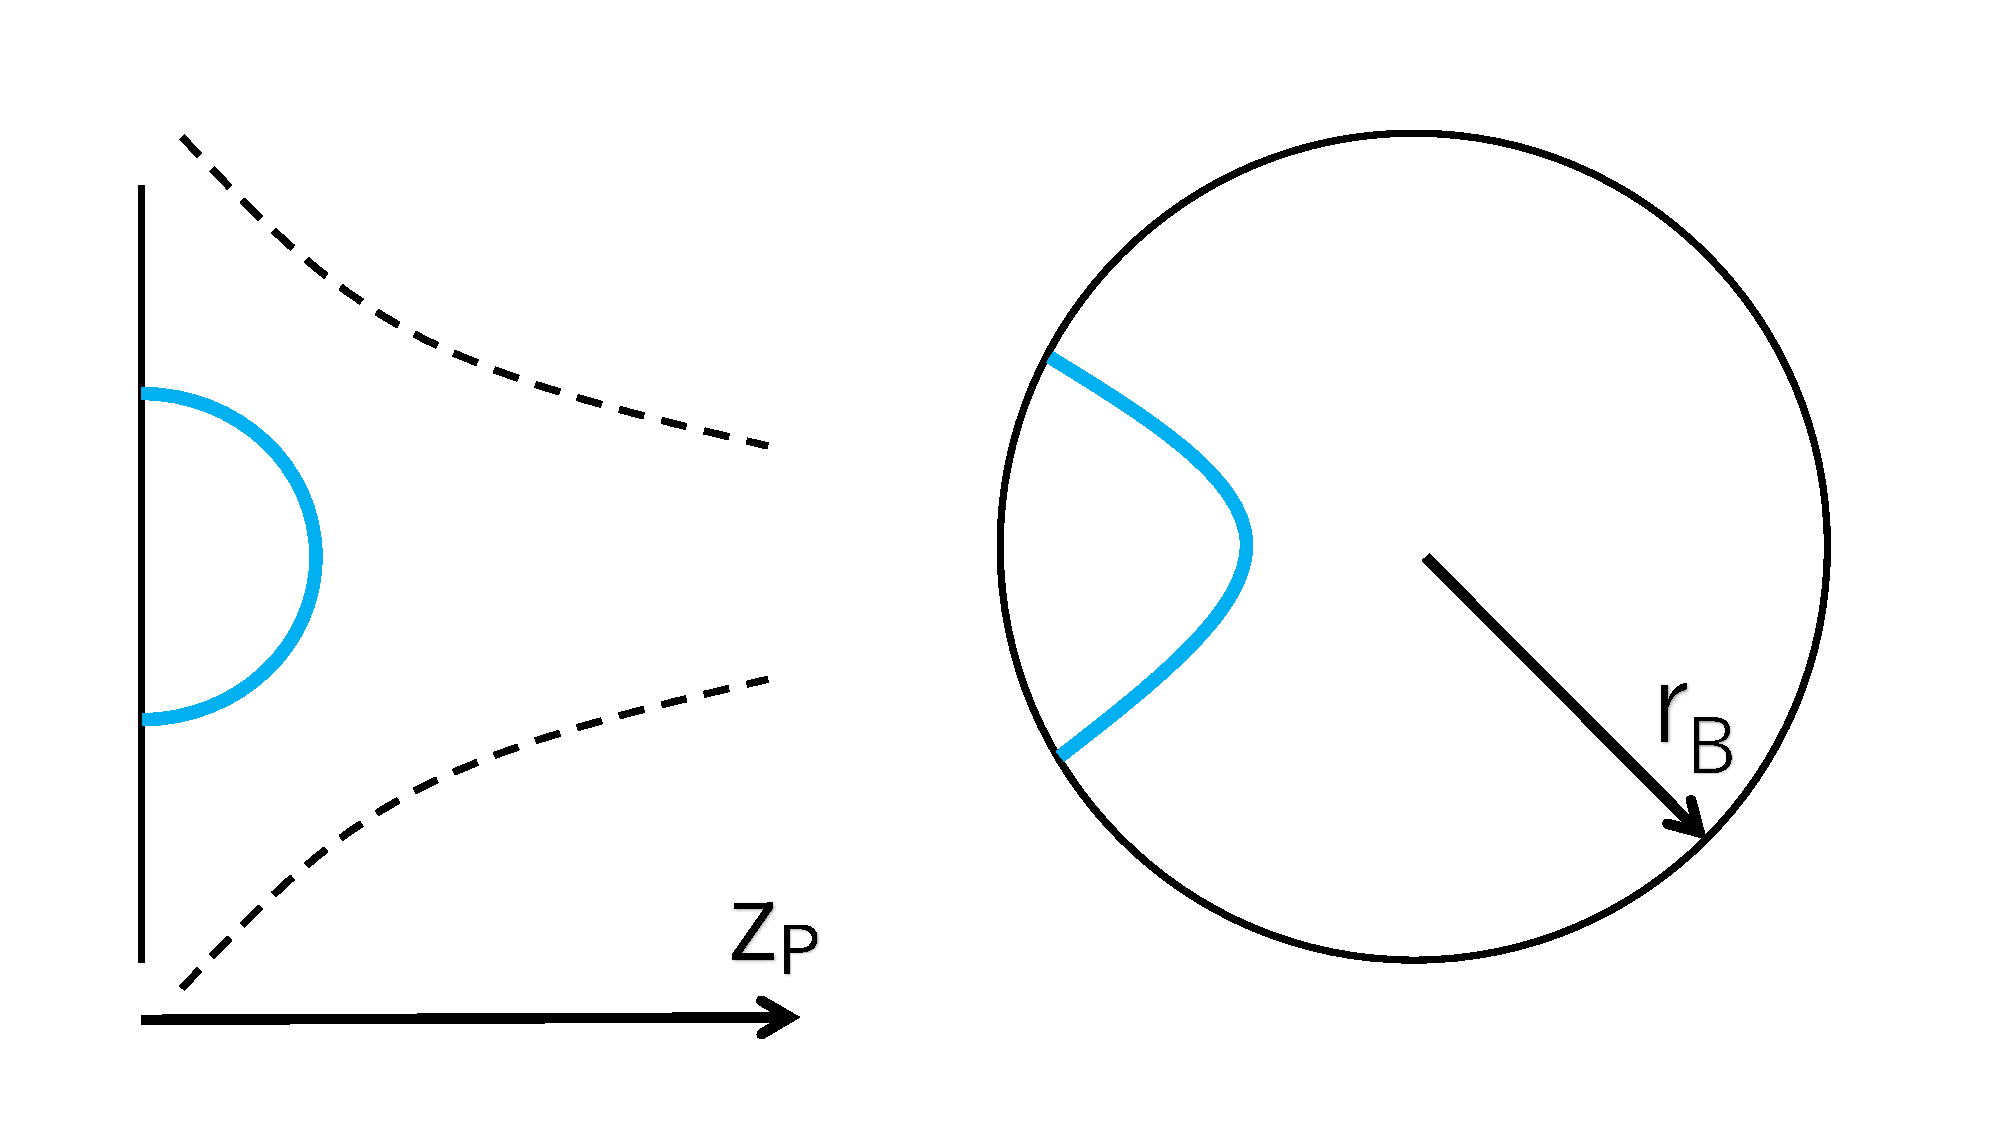
\includegraphics[width=0.7\linewidth]{adsgeod.pdf}
	\caption{Poincare座標(左)とglobal AdS座標(右)における測地線の図。}
	\label{fig:adsgeod}
\end{figure}

\subsub{non-rotating BTZブラックホールのホライズンの周りを$\varphi$方向に一周する円の長さ}
non-rotating BTZブラックホールのホライズンを$\varphi$方向に一周する円の長さは、誘導計量が$ds^2|_\text{円}=r^2d\varphi^2$となることから、
\begin{oframed}
\begin{align}
\text{length}(\text{BTZホライズンを一周する円})=2\pi r_+=2\pi R_A^2 \beta_A^{-1}\label{btzwindingcurvelength}
\end{align}
\end{oframed}
となる。
\begin{figure}[h]
	\centering
	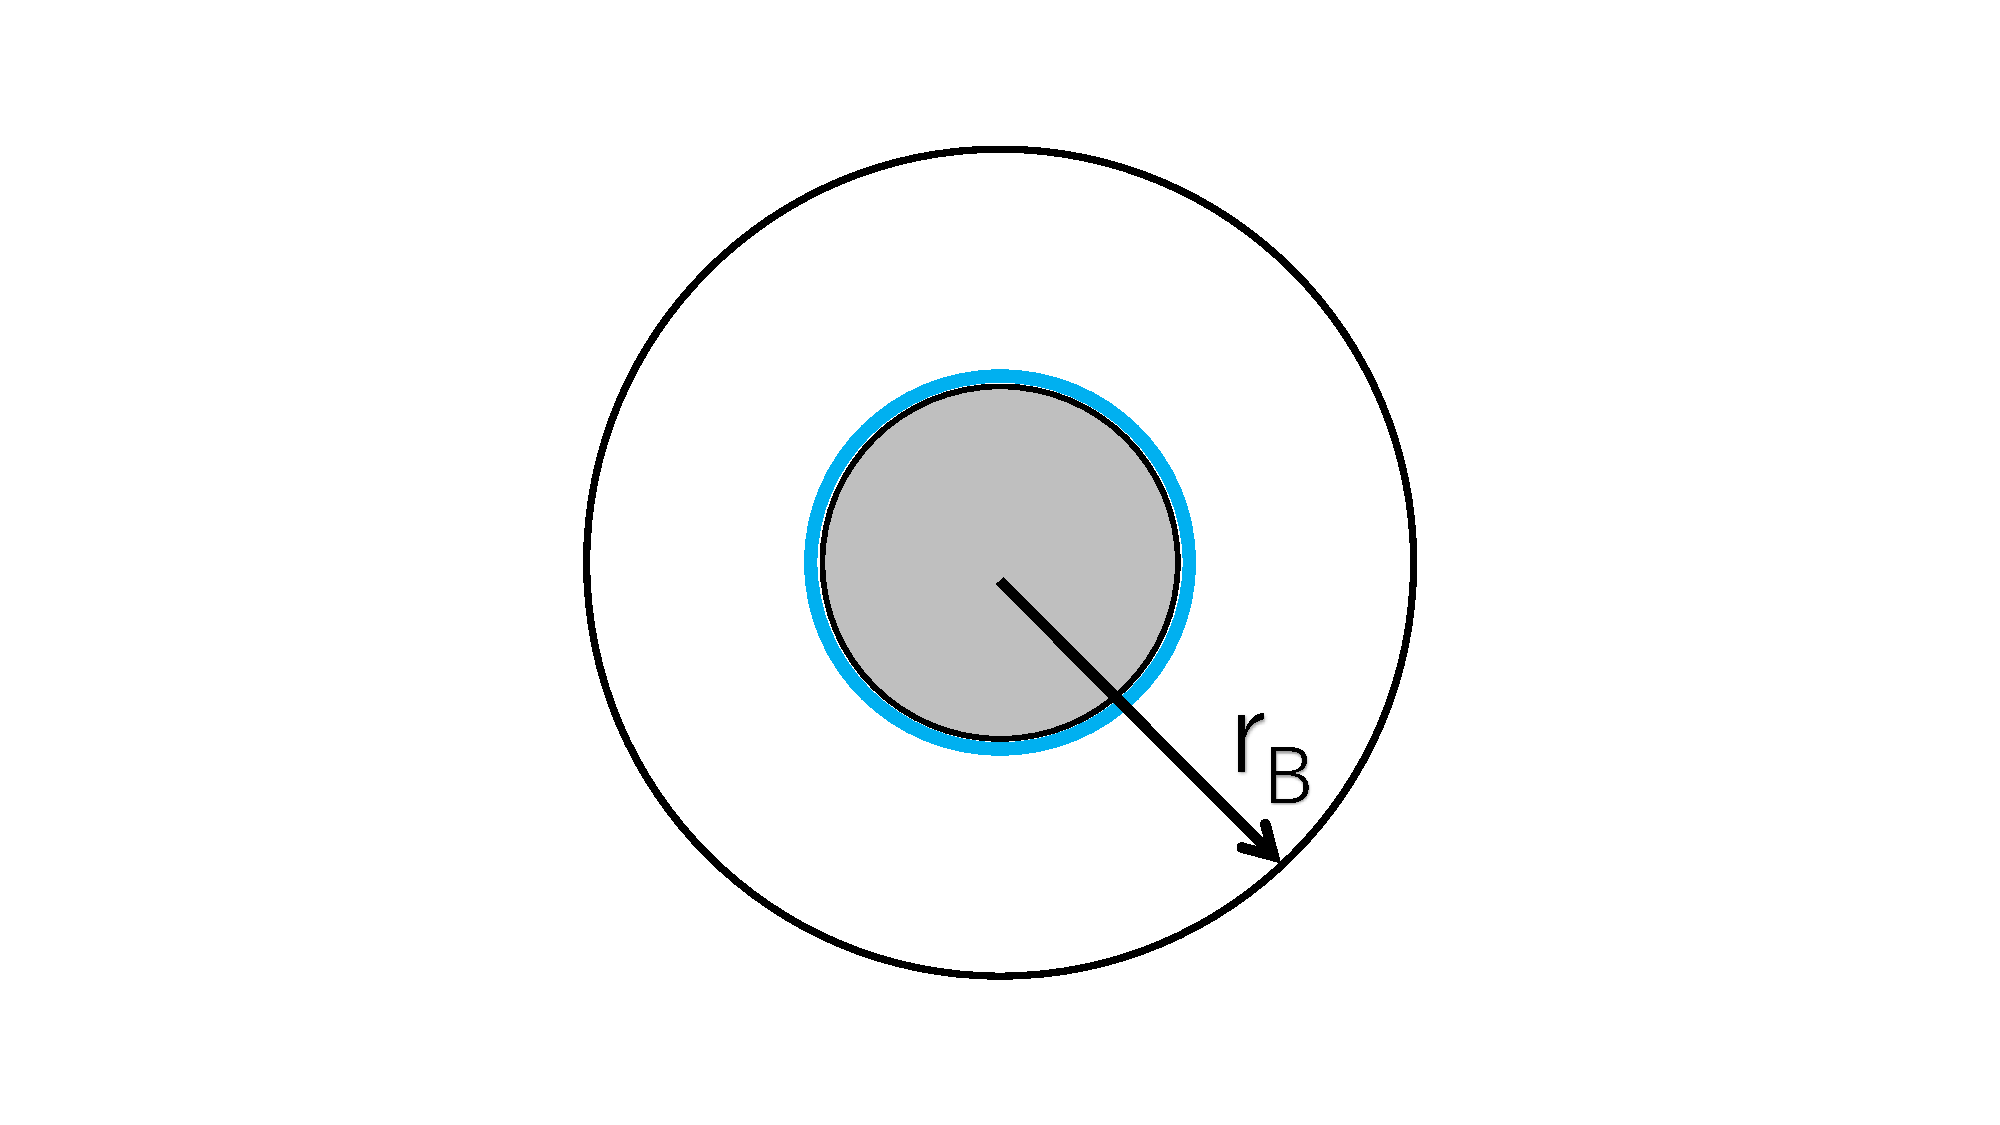
\includegraphics[width=0.7\linewidth]{BTZwindingcurve.pdf}
	\caption{non-rotating BTZブラックホールのホライズンを$\varphi$方向に一周する円の図。}
	\label{fig:BTZwindingcurve}
\end{figure}


\section{AdS$_3$/CFT$_2$対応}\label{sec:adscft}
ここでは\ref{sec:2dcft},\ref{sec:ads3}の内容を踏まえて、AdS$_3$/CFT$_2$対応を解説する。AdS/CFT対応は、一般には「AdS背景時空上の重力理論」と「AdSの``境界''上の共形場理論」の相関関数の対応を主張する。AdS/CFT対応は数学的に証明された主張ではなく、現時点では予想でしかないが、様々な具体例によって正しいことが信じられている。以下に見るように、AdS$_3$/CFT$_2$対応ではVirasoro代数の対応という非常に強力な対称性の対応関係が示唆される。

\subsection{一般論}
\subsub{AdS$_3$/CFT$_2$対応の証拠}
超弦理論から低エネルギー極限としてAdS$_3$空間を得る方法は、D1-D5ブレーン系などの構成法が知られているが、これに対応する2次元共形場理論の具体的構成はよく分かっていない。しかし、\ref{sec:2dcft},\ref{sec:ads3}節の内容から、超弦理論から天下り的に出発しなくても、AdS$_3$時空とその境界上の2次元共形場理論との対応が予想される。具体的には、以下の対応関係がその予想の根拠となる。
\begin{table}[H]
	\centering
	\begin{tabular}{|c|c|c|}\hline
		 & AdS$_3$ & CFT$_2$ \\ \hline
		大域的対称性 & $SL(2,\C)$ & $PSL(2,\C)$\\\hline
		Virasoro代数の中心電荷 & $c_A=3R_A/2G$ & $c$ \\\hline
		温度 & $\beta_A/R_A$ & $\beta$ \\\hline
		高温でのエントロピー & $(c_A/3)\pi\beta_A^{-1} R_A$ & $(c/3)\pi\beta^{-1}$ \\ \hline
	\end{tabular}
\end{table}
AdS$_3$とCFT$_2$はその大域的対称性がどちらも$SL(2,\C)$であり、その拡張として、AdS$_3$の境界に定義されたBrown-Henneaux中心電荷$c_A$のVirasoro代数はCFT$_2$の中心電荷$c$のVirasoro代数に一致することが予想される。また、高温状態のエントロピーについては、CFT$_2$についてはCardy公式から$S\sim (c/3)\pi\beta^{-1}$であり、またAdS$_3$の高温状態とはBTZ相のことだったからそのエントロピーはBekenstein-Hawkingエントロピー$(c_A/3)\pi\beta_A^{-1} R_A$である。これら2つの表式は同じ形をしており、AdS$_3$の中心電荷$c_A$とCFT$_2$の中心電荷$c$の等価性を示唆している。

\subsub{AdS$_3$に双対なCFT$_2$とは}
半古典的なAdS$_3$重力理論に双対なCFT$_2$の満たすべき条件を考える。ただし、ここで言う「双対」とは相関関数の意味での対応関係を指しており、
\begin{align}
\la e^{\int d^4x \phi(x) \mathcal{O}(x)} \ra_\text{CFT}=Z_\text{AdS}(\phi(x))
\end{align}
が成り立つようなCFT$_2$とはどのようなものかを考える。この式はAdS$_{d+1}$/CFT$_d$対応を表す基本的な式で、\textbf{GKPW(Gukov-Klebanov-Polyakov-Witten)公式}\cite{Gubser_1998}\cite{Witten:1998qj}と呼ばれている。

AdS$_3$重力理論での半古典極限とは、AdS半径がPlanck長よりも十分大きい$R_A\gg G$の極限である。このときBrown-Henneauxの関係式によって$c_A$がCFT$_2$の$c$に一致することを仮定すれば、$R_A\gg G$の半古典極限はCFT$_2$において中心電荷が$c\gg 1$となる極限に対応する。したがって、(半)古典重力双対を持つような2次元共形場理論の中心電荷は$c\gg 1$を満たすと予想される。

またGKPW公式から、CFT$_2$の状態と半古典AdS$_3$重力理論の状態が対応する。重力理論の半古典極限においてその量子的ゆらぎは非常に小さく、重力理論の基底状態(=Einstein方程式の解)と励起状態のエネルギー差は非常に大きい。したがってこれに対応するCFT$_2$のエネルギー固有値のスペクトルも、基底状態と励起状態とで大きなエネルギー差を持ち、``sparse''なスペクトルを持つと予想される。

したがって古典重力双対を持つような2次元共形場理論は少なくとも、「$c\gg 1$」でありかつ「sparseなスペクトル」を持つと予想される。

\subsection{状態と時空の対応}
GKPW公式は、CFT$_2$の基底状態と(古典)AdS$_3$時空の対応を述べている。直線/円周上のCFT$_2$のカノニカル分布に、相関関数の意味で対応する漸近的AdS$_3$時空は以下のものになる。ここで「直線/円周上の共形場理論」と書いたとき、空間$x$方向が直線/円周となっている共形場理論を指すことにする。例えば、円筒上の共形場理論の温度$\beta$のカノニカル分布$e^{\beta H}$に対応するRiemann面は、$x$方向が半径$L$にコンパクト化され、$\tau$方向が半径$\beta$にコンパクト化されたトーラスに対応する。
\begin{table}[H]
	\centering
	\begin{tabular}{|c|c|}\hline
		CFT$_2$ & AdS$_3$ \\ \hline
		円周上の高温状態$e^{-\beta H},\ \beta<1$ & thermal non-rotating BTZ \\\hline
		円周上の低温状態$e^{-\beta H},\ \beta>1$ & thermal AdS \\\hline
		直線上の真空 & Poincare座標(global AdSの半分) \\\hline
		\multirow{2}{*}{直線上の有限温度状態$e^{-\beta H}$} & Poincare座標の$z=z_H$にホライズンを持つ\\
		& ブラックホール(non-rotating BTZの半分) \\ \hline
	\end{tabular}
\end{table}

\section{AdS/BCFTの処方}\label{sec:adsbcft}
ここでは境界つき2次元多様体上の境界共形場理論(BCFT)に対するAdS/CFT対応を考える。

\subsection{AdS/BCFTの処方}
\cite{Takayanagi:2011zk}で提案されたAdS/BCFTの処方では、境界共形場理論に双対な境界付きAdS重力を、BCFTの境界に対応する境界$Q$ (図\ref{fig:adsbcft})についてNeumann境界条件を課して決める。ただし、CFTが現れる$r\to \infty$の境界$M$ (図\ref{fig:adsbcft})では通常のAdS/CFT対応と同様にDirichlet境界条件を課す。
\begin{figure}[h]
	\centering
	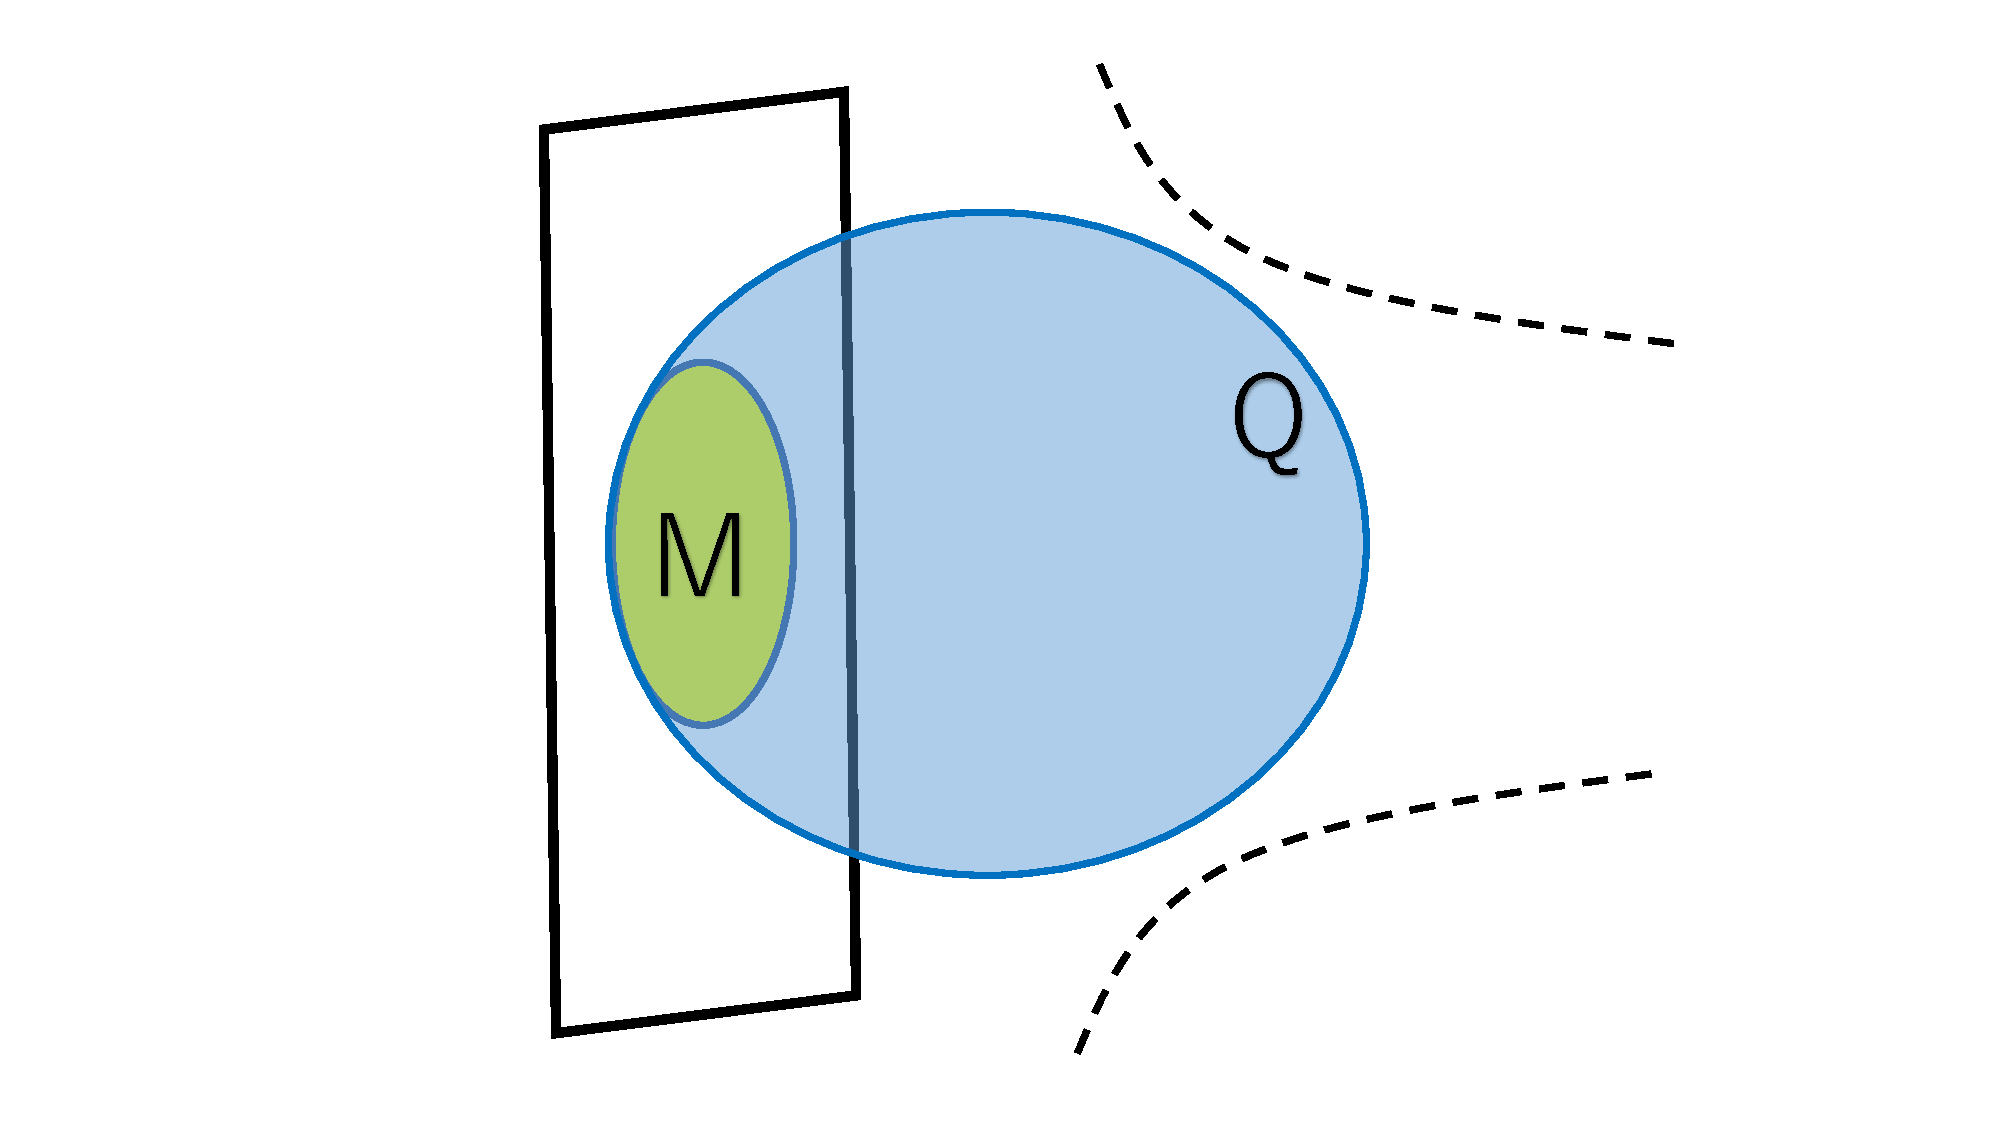
\includegraphics[width=0.7\linewidth]{adsbcft.pdf}
	\caption{黄色の領域がBCFTを表しており、青色の領域が双対な境界付きAdS$_3$時空を表している。$M$は$r\to\infty$の漸近的な境界のことであり、$Q$はBCFTの境界に対応するAdS$_3$の境界である。}
	\label{fig:adsbcft}
\end{figure}

Neumann境界条件を変分法で課すためには、通常Dirichlet境界条件に用いたGibbons-Hawking項\cite{York:1972sj}\cite{Gibbons:1976ue}を$1/2$倍して、
\begin{align}
S[g]=\frac{1}{16\pi G}\left(\int_\text{内部} \sqrt{-\det g}(R-2\Lambda) + \int_Q \sqrt{-\det h}K\right)
\end{align}
という作用を用いればよい\cite{Krishnan:2016mcj}。ただし$h$は境界$Q$上の誘導計量で、$Q$の単位法線ベクトルを$n$とすれば$h_{\mu\nu}=g_{\mu\nu}-n_\mu n_\nu$で定まる。また$K_{\mu\nu}=\nabla_\mu n_\nu$は外曲率(extrinsic curvature)と呼ばれ、さらに$K=h_{\mu\nu}K^{\mu\nu}$と書いた。

$Q$上の単位接ベクトルを$e_a\ (a=1,\ldots, \dim Q)$で表し$K_{ab}=e_a^\mu e_b^\nu K_{\mu\nu}$と書く。
このとき作用の変分は
\begin{align}
\delta_g S[g]&=\frac{1}{16\pi G}\left(\int_\text{内部} \sqrt{-\det g} \left( R^{\mu\nu}-\frac{1}{2}g^{\mu\nu}R+\Lambda g^{\mu\nu} \right)\delta g_{\mu\nu}\right.\notag\\
&\left.+\frac{1}{2}\int_\text{Q} \sqrt{-\det h}h^{ab}\delta (K_{ab}-h_{ab}K)\right)
\end{align}
となり、$Q$でのNeumann境界条件
\begin{align}
K_{ab}-h_{ab}K=0
\end{align}
が課される。より一般には$S[g]$に$h$のみに依存する境界項$S_0[h]$を加える自由度がある。そこでBrown-Yorkテンソル\cite{Brown:1992br}と同様に、$S_0[h]$についてのエネルギー運動量テンソル
\begin{align}
T^Q_{ab}=\frac{2}{\sqrt{-\det h}}\frac{\delta S_0[h]}{\delta h^{ab}}
\end{align}
と定義すると、$Q$についてのより一般的な境界条件として
\begin{align}
K_{ab}-h_{ab}K=16\pi G T_{ab}^Q
\end{align}
を得る。

\subsection{具体例}
\subsub{上半平面}
上半平面$\UHP$上の境界共形場理論に対応する境界付きAdS$_3$時空はどのようなものだろうか。$\UHP$上の境界共形場理論は、二重化のトリックを用いることで、Virasoro対称性が半分保たれた平面$\C$上の共形場理論に拡張できた。共形場理論のVirasoro代数はAdSの境界のVirasoro代数に対応するので、$\UHP$に対応する境界付きAdS空間として、上半分のPoincare AdS
\begin{align}
ds^2=R_A^2 \frac{dz^2+d\tau^2+dx^2}{z^2},\quad \tau,z>0
\end{align}
が対応すると自然に予想できる(図\ref{fig:uhpadsbcft})。
\begin{figure}[h]
	\centering
	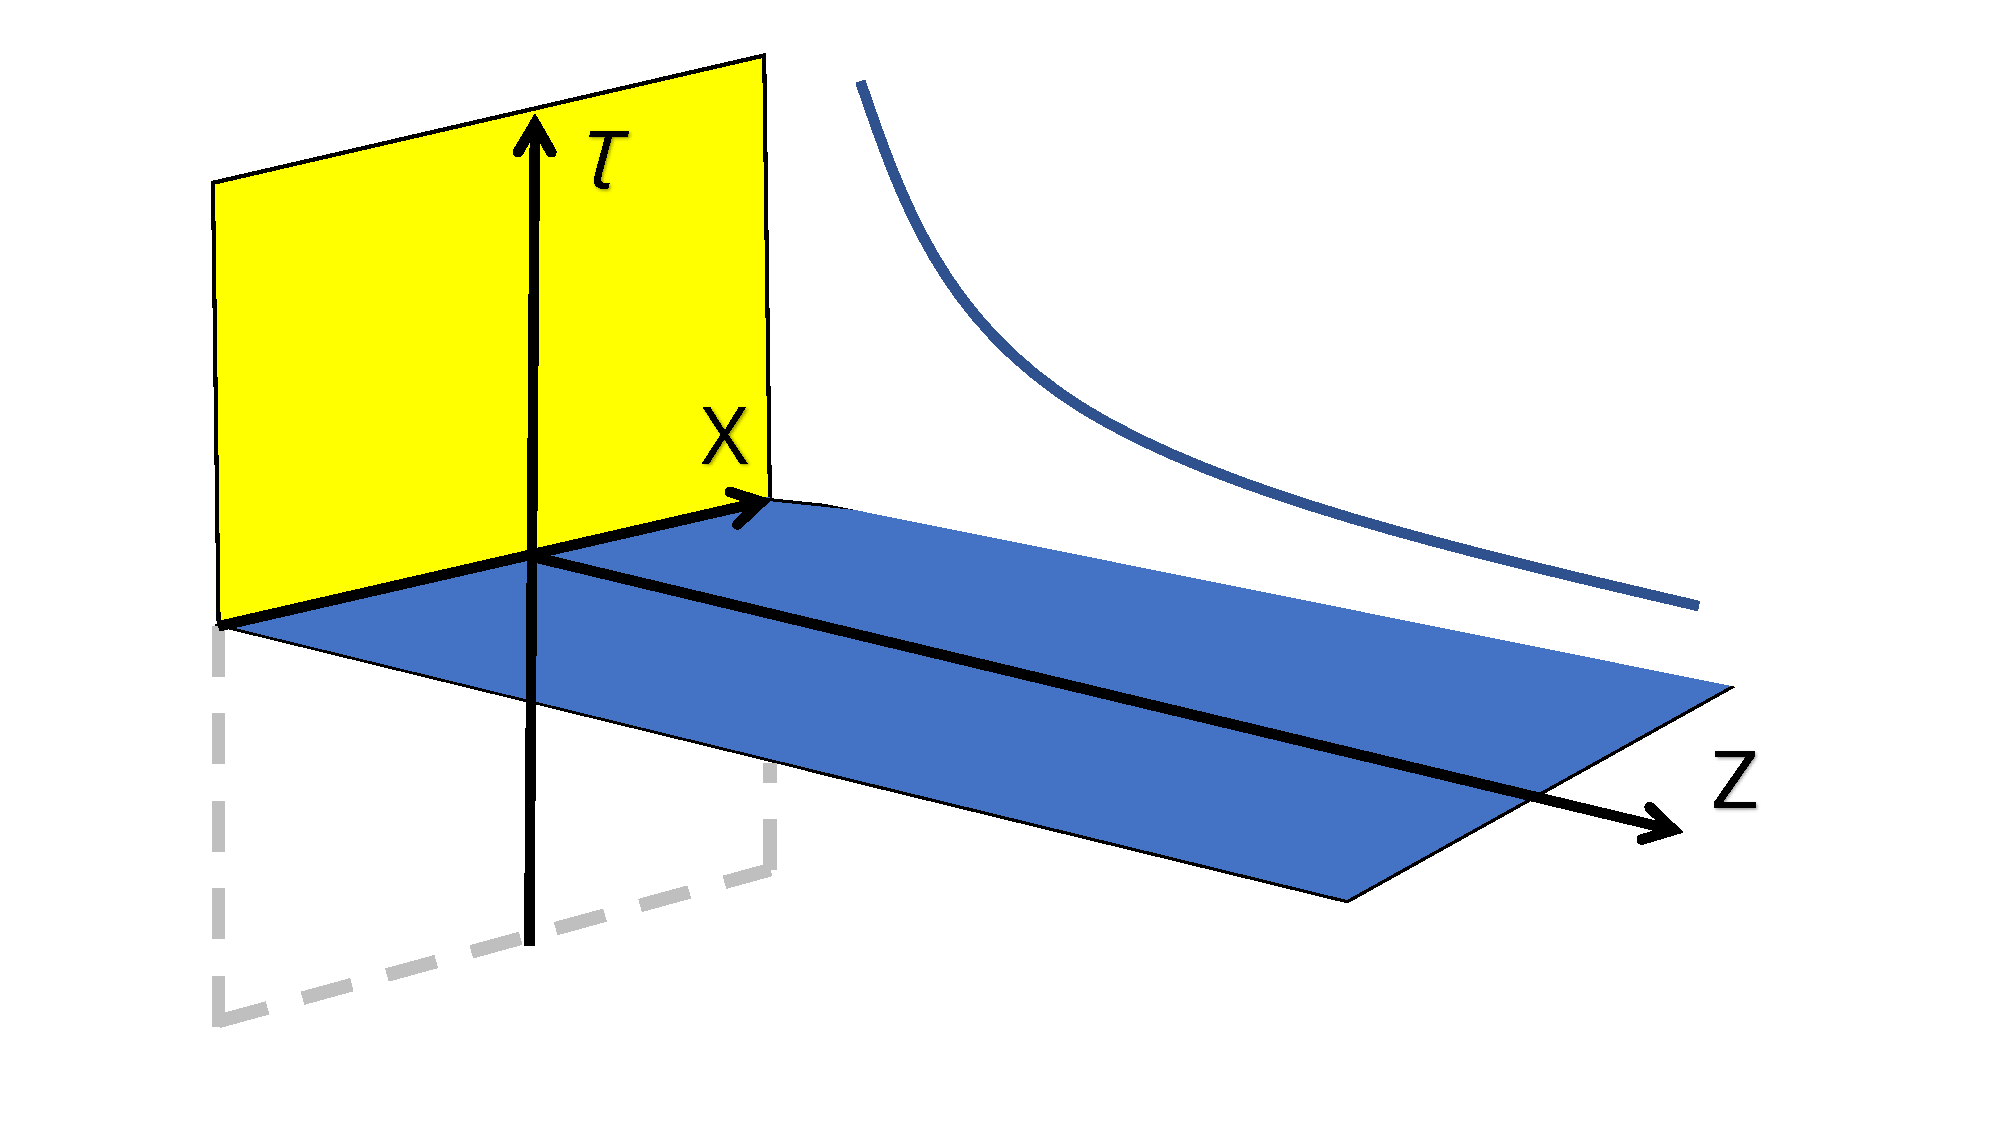
\includegraphics[width=0.7\linewidth]{UHPadsbcft.pdf}
	\caption{上半平面$\UHP$上の境界共形場理論に対応する境界付きAdS$_3$時空の図。黄色の領域がBCFTを表しており、青色の平面はBCFTの境界に対応するAdS$_3$の境界$Q$を表している。}
	\label{fig:uhpadsbcft}
\end{figure}

このとき時空の境界$Q$は$\tau=0$平面となっていて、$Q$上で常に$K_{ab}=0$となるから、たしかにNeumann境界条件$K_{ab}-h_{ab}K=0$を満たしている。

\subsub{有限の長さの円筒}
$z=-\pi/2,\pi/2$に境界をもち、$z\sim z+2\pi i\beta$と同一視の入った有限の長さの円筒$[-\pi/2,\pi/2]\times S_{\beta}^1$についても、二重化の方法を用いればトーラス$S^1\times S_{\beta}^1$に拡張できる。

$r\to \infty$での境界をトーラスに持つようなユークリッド符号のAdS$_3$時空は、thermal AdS$_3$とthermal non-rotating BTZの2つがあり、温度$\beta$によってどちらに対応するかが決まる。
\begin{description}
\item[$\beta>1$のとき] \hfill\\
$\beta>1$の低温では、thermal AdS$_3$がトーラスに対応する時空となる。したがって、円筒$[-\pi/2,\pi/2]\times S_{\beta}^1$に対応する時空は(\ref{adsbcftTAdSmetric})から、
\begin{align}
ds^2&=(r^2-\beta_A^2)d\varphi^2+\frac{R_A^2}{r^2-\beta_A^2}dr^2+r^2d\tau^2\\
&\tau\sim \tau+2\pi,\quad -\frac{\pi R_A}{2\beta_A}<\varphi <\frac{\pi R_A}{2\beta_A}
\end{align}
となる。ただし、モジュラー変換によって時間$\tau$と空間$\varphi$が入れ替わるので、\ref{adsbcftTAdSmetric}での$\tau',\varphi'$をそれぞれ$\varphi,\tau$と書いている。$R_A/\beta_A<1$より、$\tau$方向がトーラスの大円をなし、$\varphi$方向がトーラスの小円をなす。この時空は$1$つの連結成分をもつ境界$Q$を持ち、図のようになる。
\begin{figure}[h]
	\centering
	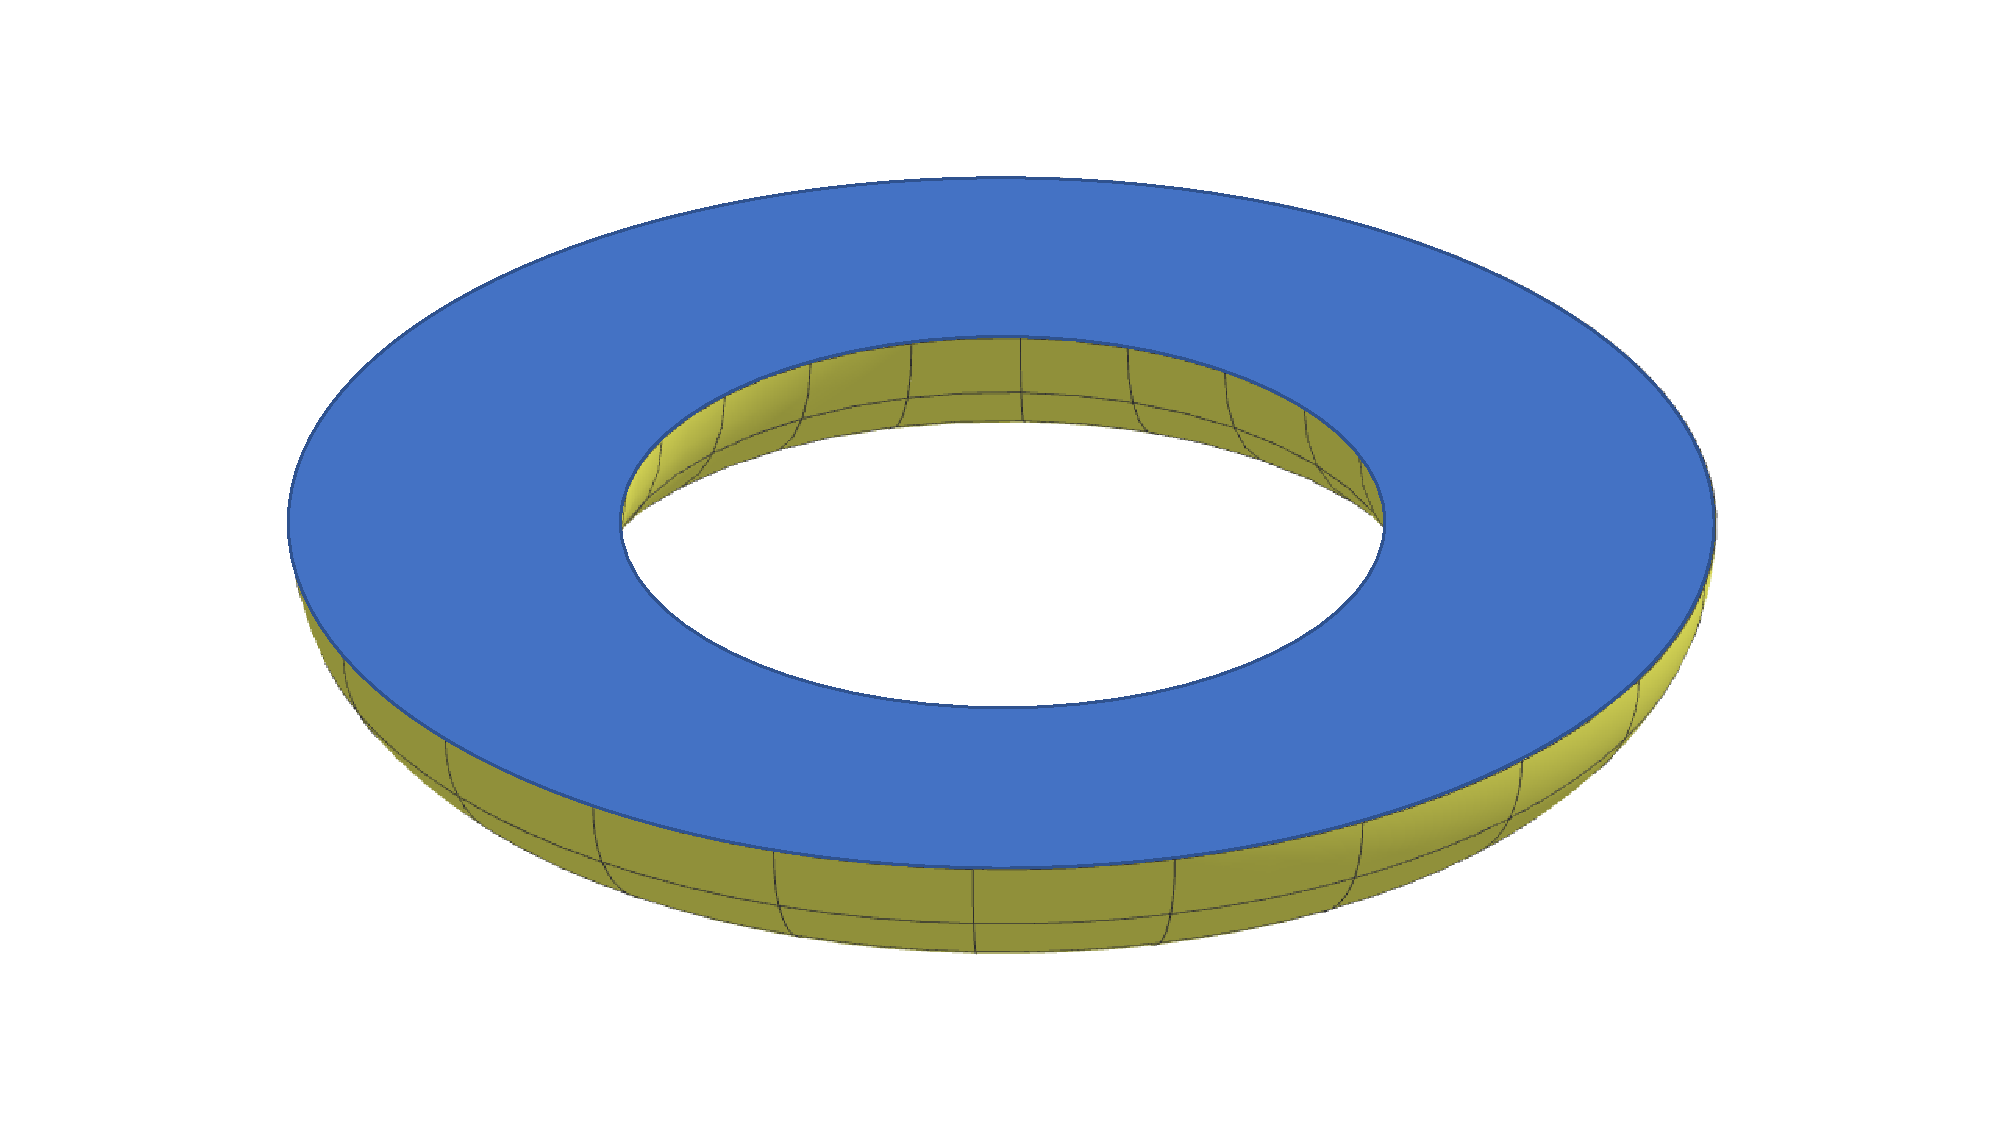
\includegraphics[width=0.7\linewidth]{adsbcftTAdS.pdf}
	\caption{$\beta>1$の円筒に対応する、$1$つの境界を持ったAdS時空。$\varphi=\pm\pi/2$に$1$つの境界$Q$(青い面)を持ち、トーラスの小円の動径方向が$r$軸に対応している。}
	\label{fig:adsbcfttads}
\end{figure}

\item[$\beta<1$のとき] \hfill\\
$\beta<1$の高温では、thermal non-rotating BTZがトーラスに対応する時空となる。したがって、円筒$[-\pi/2,\pi/2]\times S_{\beta_A}^1$に対応する時空は(\ref{adsbcftBTZmetric})から、
\begin{align}
ds^2&=(r^2-(R_A^2\beta_A^{-1})^2)d\tau^2+\frac{R_A^2}{r^2-(R_A^2\beta_A^{-1})^2}dr^2+r^2d\varphi^2\\
&\tau\sim \tau+2\pi\frac{\beta_A}{R_A},\quad -\frac{\pi}{2}<\varphi<\frac{\pi}{2} 
\end{align}
となる。$\beta_A/R_A<1$より、$\phi$方向がトーラスの大円をなし、$\tau$方向がトーラスの小円をなす。。この時空は$2$つの連結成分をもつ境界$Q$を持ち、図\ref{fig:adsbcftbtz}のようになる。
\begin{figure}[h]
	\centering
	\begin{tabular}{c}
	\begin{minipage}{0.50\hsize}
		\centering
		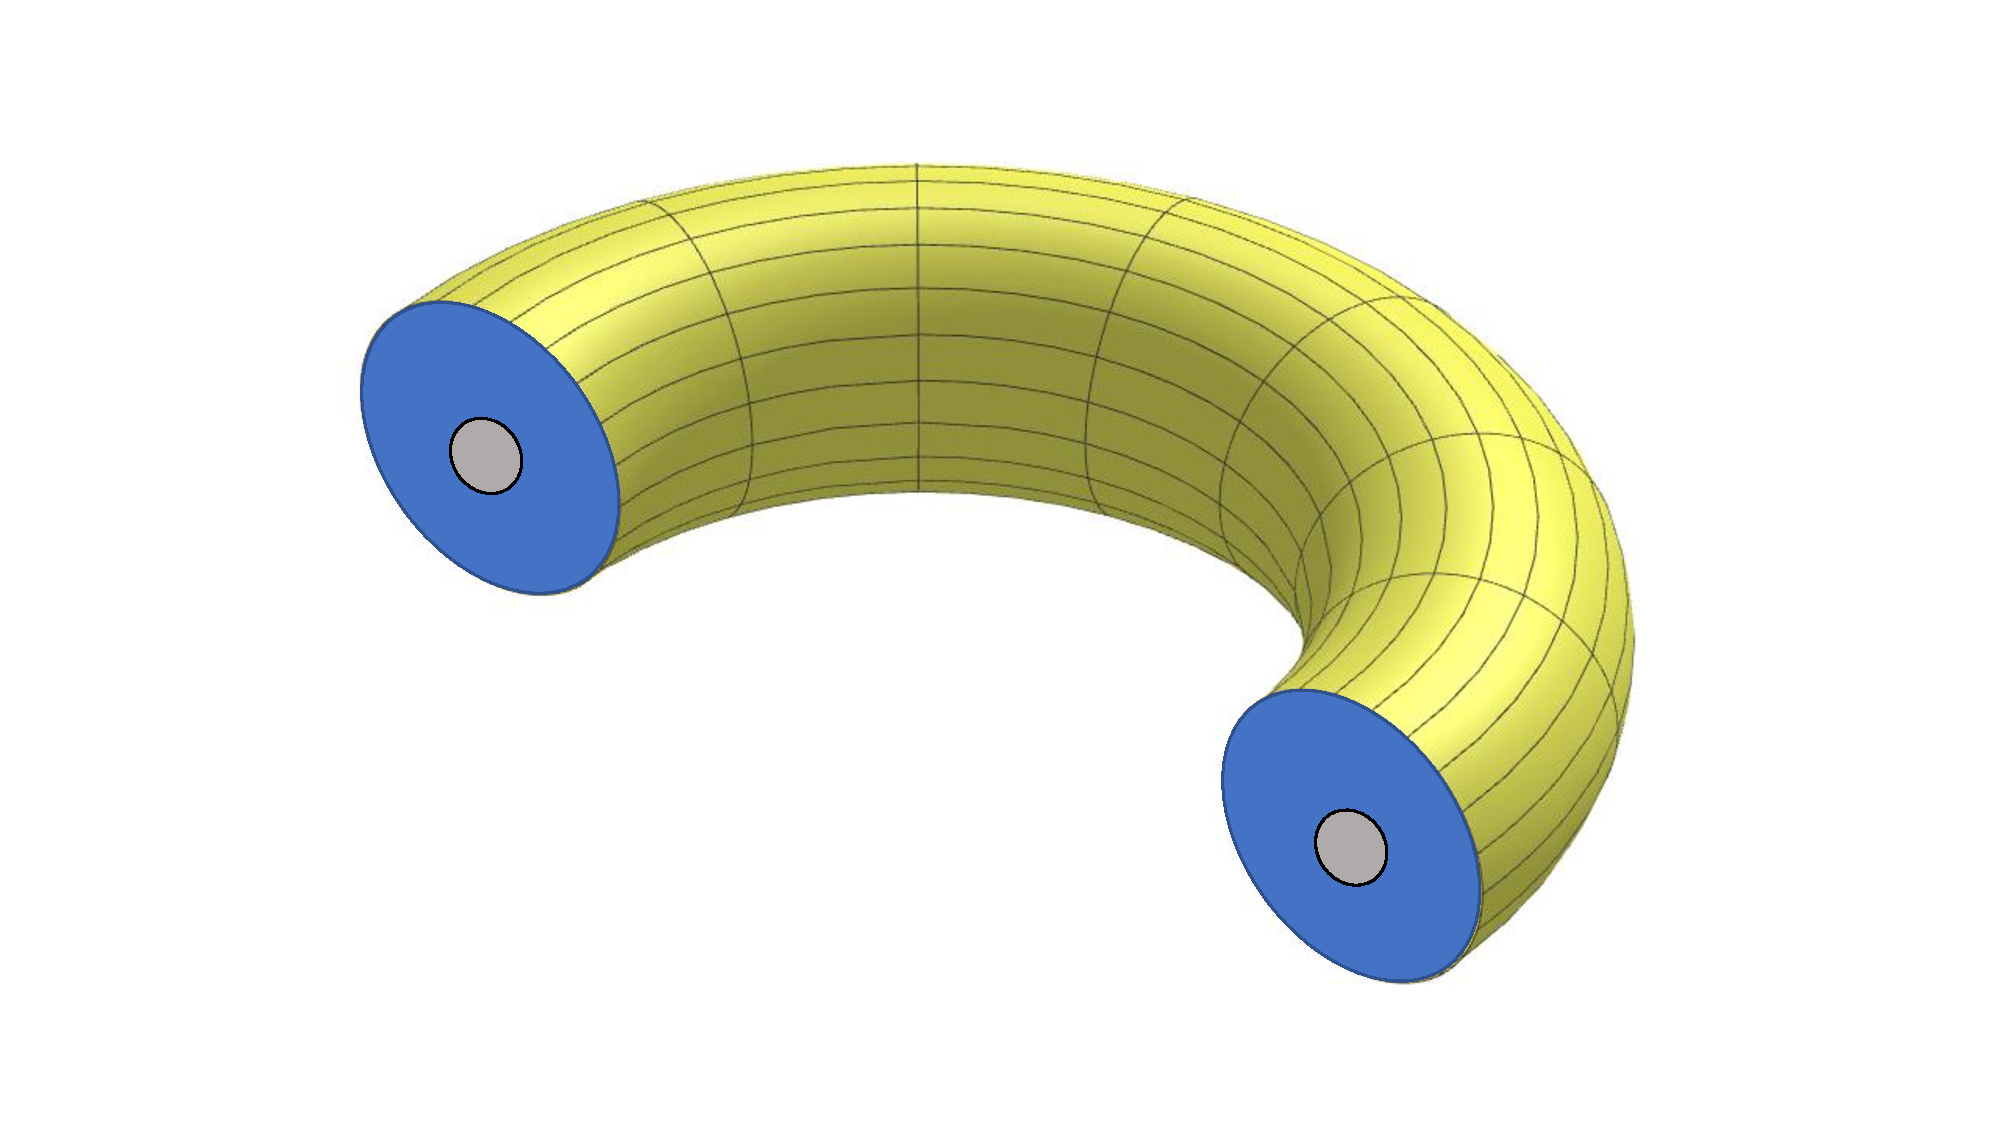
\includegraphics[width=\linewidth]{adsbcftBTZ.pdf}
		\caption{$\beta<1$の円筒に対応する、$2$つの境界を持ったAdS時空。$\varphi=\pm\pi/2$に$2$つの境界$Q$(青い面)を持ち、トーラスの小円の動径方向が$r$軸に対応している。灰色の領域はBTZブラックホールのホライズン内部を表しており、この領域で計量は定義されていない。}
		\label{fig:adsbcftbtz}
	\end{minipage}
	\begin{minipage}{0.50\hsize}
		\centering
		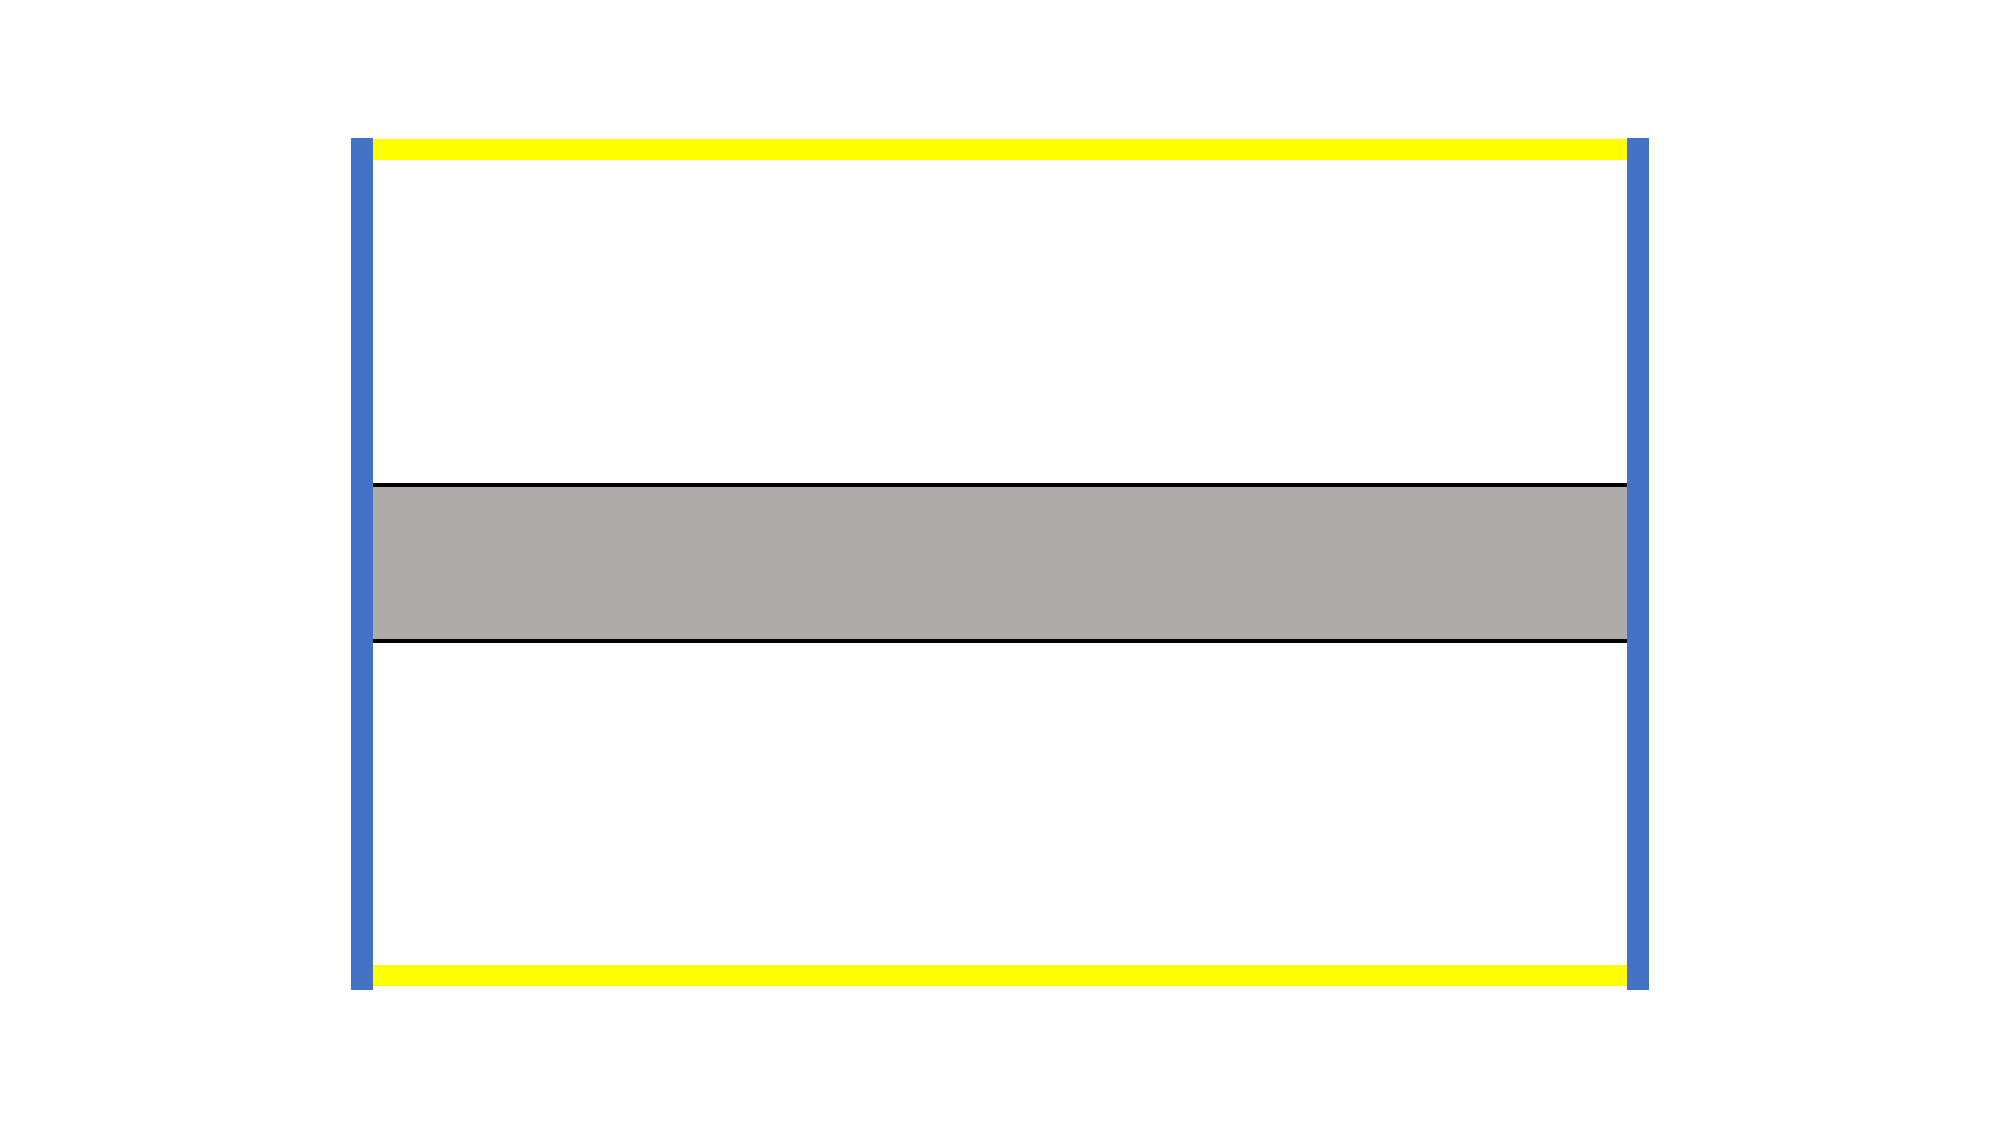
\includegraphics[width=\linewidth]{adsbcftBTZsection.pdf}
		\caption{左図の$\tau=0,\pi\beta/R_A$面での断面図。$\varphi=\pm\pi/2$に境界$Q$(青い直線)を持つ。灰色の領域はBTZブラックホールのホライズン内部を表しており、この領域で計量は定義されていない。黄色の半円は$r\to \infty$の境界を表している。}
		\label{fig:adsbcftbtzsection}
	\end{minipage}
	\end{tabular}
	
\end{figure}

\end{description}

	\chapter{2次元共形場理論におけるエンタングルメントエントロピー}\label{chap:EEreview}
この章では2次元共形場理論におけるエンタングルメントエントロピーに焦点をあてて、本研究の内容を説明するために必要な事項を解説する。
\newline

合成系の量子論における基礎的な現象である\textbf{エンタングルメント(entanglement)}は、1935年にEinstein, Podolsky, Rosenによって提案された思考実験\cite{EPR1935}を発端に1982年にAspect, Dalibard, Roger\cite{Aspect1982}らによって実験的に確認され、量子情報理論の分野で理論的に整備されてきた。エンタングルメントやその度合いを定量化する量は様々な分野において様々な文脈で応用・研究されている。例えば量子情報理論においては量子計算や量子誤り訂正を行うための源として応用されたり\cite{HayashietalQI}\cite{nielsen_chuang_2010}、相対論的な場の理論においてはある種の``閉じ込め"が起きて内部の情報にアクセスできなくなった系の熱力学を考える上で重要視されていたり、物性理論においてはトポロジカルな相構造の検出\cite{Kitaev2006}\cite{Levin_2006}や非平衡過程の熱力学的性質を調べるため\cite{Sagawa}\cite{Calabrese_2016}に用いられていたりする。この章では、相対論的な場の理論に焦点を当てて、エンタングルメントの性質を見ていく。

2次元共形場理論は中心電荷$c$によってその性質は大きく変わり、$c<1$のミニマルモデルや$c=1$の自由場は、物性理論での可解格子模型の連続極限にあると考えられているのに対し、$c\gg 1$で重力双対を持つような共形場理論は非常にカオス性の強い理論であると考えられている\cite{Maldacena:2015waa}。そのためエンタングルメントエントロピーの性質も中心電荷によって異なる。特に$c\gg 1$で重力双対を持つような2次元共形場理論でのエンタングルメントエントロピーを相関関数から計算することは難しいが、AdS$_3$/CFT$_2$対応によってAdS$_3$空間での測地線の長さを計算することに対応づけられる。この対応公式は\textbf{笠-高柳公式(Ryu-Takayanagi formula)}\cite{Ryu:2006ef}として知られており、AdS$_3$/CFT$_2$対応やBekenstein-Hawkingエントロピーの面積則への理解につながる公式としてだけでなく、臨界点上の強結合系におけるエンタングルメントの解析にも用いられるなど、様々な応用が考えられている。
\newline

\ref{sec:entanglement},\ref{sec:unruh}節では、エンタングルメントの定義と、場の理論の真空のエンタングルメントの具体例であるUnruh効果を\cite{Ohya}\cite{TakayanagiJapan}\cite{Hotta}\cite{Iso}\cite{Birrell:1982ix}\cite{Crispino:2007eb}\cite{Nishioka:2018khk}を参考にして解説する。\ref{sec:EE},\ref{sec:EEcft2},\ref{sec:RTformula}節では、2次元共形場理論でのエンタングルメントエントロピーの計算方法やその性質を\cite{TakayanagiJapan}\cite{Nishioka:2018khk}\cite{Rangamani:2016dms}\cite{Takayanagi:2012kg}\cite{wu2019ads3}\cite{Calabrese:2004eu}\cite{Calabrese:2009qy}を参考にして解説する。

\section{エンタングルメント}\label{sec:entanglement}
ここでは\ref{sec:unruh}節以降で、場の量子論の状態がもつエンタングルメントを扱う準備として、エンタングルメントの定義を説明する。エンタングルメントは合成系の量子力学で現れる、非局所的な性質をもった現象であり、場の量子論のおいては真空ですらエンタングルメントの構造がある。このことはブラックホールのHawking放射のモデルにおいて本質的な役割を果たし、量子重力理論の性質を調べる上で重要な鍵になると期待されている。

\subsection{有限次元量子力学におけるエンタングルメント}
\subsub{状態}
有限次元複素ヒルベルト空間$\HH=\C^d$で表される量子系の\textbf{状態(state)}、あるいは\textbf{密度行列(density matrix)}$\rho\in M_d(\C)$とは
\begin{align}
\rho \geq 0,\  \rho^\dagger = \rho,\  \tr \rho=1
\end{align}
となる行列のことである。とくに階数$1$の状態$\rho$を\textbf{純粋状態(pure state)}といい、その固有ベクトル$\psi$でノルムが$1$のものをとれば$\rho=\psi\psi^\dagger$と書ける。この$\psi\in\C^d$のことも純粋状態と呼ぶ。純粋状態でない状態を\textbf{混合状態(mixed state)}という。状態全体の集合は凸集合をなし、純粋状態はその端点になっている。したがって混合状態は必ず純粋状態の凸結合に分解できる。
\begin{ex}
	系にハミルトニアン$H\geq 0$が与えられたとき、カノニカル分布$\rho_\beta=e^{-\beta H}/Z(\beta)$は混合状態である。ただし$Z(\beta)=\tr e^{-\beta H}$と書いた。$H$の固有ベクトル$H|i\ra=E_i|i\ra$をとれば、
	\begin{align}
	\rho_\beta=\frac{e^{-\beta H}}{Z(\beta)}=\sum_{i}\frac{e^{-\beta E_i}}{Z(\beta)}|i\ra\la i|
	\end{align}
	となる。これは純粋状態$|i\ra\la i|$の凸結合による$\rho_\beta$の分解になっている。
\end{ex}

\subsub{エンタングル状態}
有限次元複素ヒルベルト空間$\HH_A=\C^m, \HH_B=\C^n (m,n\geq2)$上に記述される系$A,B$に対して、その合成系$A+B$のヒルベルト空間として$\HH=\HH_A\tensor \HH_B=\C^m\tensor \C^n$を考える。ただし$\HH$の内積は$\HH_A,\HH_B$の内積$\la,\ra_A,\la,\ra_B$を用いて、
\begin{align}
\la \psi_A\tensor \psi_B, \phi_A\tensor \phi_B\ra = \la\psi_A,\phi_A\ra_A \la\psi_B,\phi_B\ra_B\ (\psi_A,\phi_A\in \HH_A,\ \psi_B,\phi_B\in \HH_B)
\end{align}
と定めたものを線形拡張して定義する。\footnote{ちなみにヒルベルト空間の直和$\HH_A\directsum \HH_B$は、ベクトル空間としての直和に\[\la \psi_A\tensor \psi_B, \phi_A\tensor \phi_B\ra = \la\psi_A,\phi_A\ra_A +\la\psi_B,\phi_B\ra_B\ (\psi_A,\phi_A\in \HH_A,\ \psi_B,\phi_B\in \HH_B)\]で内積を入れたものである。
}
\begin{oframed}
$\HH_A,\HH_B$の純粋状態$\psi_A,\psi_B$(ノルム$1$のベクトル)のテンソル積$\Psi=\psi_A\tensor\psi_B$はノルム$1$であり、$\HH$の純粋状態となる。このように、$\HH$の純粋状態$\Psi$であって、$\HH_A,\HH_B$のある純粋状態$\psi_A,\psi_B$が存在して$\Psi=\psi_A\tensor\psi_B$と書けるようなものを、\textbf{セパラブル状態(separable state)}という。逆に、$\HH$のセパラブル状態でない純粋状態を\textbf{エンタングル状態(entangled state)}という。
\end{oframed}

$\HH_A,\HH_B$の正規直交基底$\psi_A^i,\psi_B^j$をとれば、Hilbert空間のテンソル積の定義から$\HH$の元を$\Psi=\sum_{i} c_{ij}\psi_A^i \tensor \psi_B^j$と展開できる。展開係数行列$C=(c_{ij})$を極分解して$C=UDV$  ($U,V$はユニタリー行列、$D$は対角行列)と分解できるので、正規直交基底を$\psi_A'=U^T \psi_A, \psi_B'=V\psi_B$と取り換えると、$\Psi=\sum_{i} d_{i}\psi_A^{'i} \tensor \psi_B^{'i}$と、対角的に展開できる。この展開を\textbf{Schmit展開}という。
このとき、展開係数行列$(d_i)$の階数が$1$であることと$\Psi$がセパラブル状態であることは同値である。

\begin{ex}
$\C^2$の基底を$|0\ra, |1\ra$ととると、次の$\HH=\C^2\tensor\C^2$の純粋状態はエンタングル状態である。
\begin{align}
\frac{|0\ra_A|0\ra_B\pm |1\ra_A|1\ra_B}{\sqrt{2}},\ \frac{|0\ra_A|1\ra_B\pm |1\ra_A|0\ra_B}{\sqrt{2}}
\end{align}
特に$(|0\ra_A|0\ra_B+ |1\ra_A|1\ra_B)/\sqrt{2}$は\textbf{EPR(Einstein-Podolsky-Rosen)状態}と呼ばれる。
\end{ex}

\begin{ex}\label{generalentangledstate}
$\HH=\C^d\tensor \C^d$の純粋状態
\begin{align}
|\Psi\ra=\sum_{i=1}^d a_i|i\ra_A |i\ra_B\quad \left(\sum_{i=1}^d a_i^2=1, a_1\neq 0, a_2\neq 0 \right)
\end{align}
はエンタングル状態である。特に$a_1=\cdots=a_d=1/\sqrt{d}$のときの状態を最大エンタングル状態(maximally entangled state)という。
\end{ex}

\begin{ex}
$\HH$上のカノニカル分布$\rho_\beta=e^{-\beta H}/Z(\beta)$に対して、$\HH$を``2倍"したヒルベルト空間$\HH_L\tensor \HH_R,\ \HH=\HH_L=\HH_R$を考え、その上の\textbf{thermofield double状態}を
\begin{oframed}
\begin{align}
\sum_{i} \frac{e^{-\beta E_i/2}}{\sqrt{Z(\beta)}}|i\ra_L |i\ra_R \in \HH_L\tensor\HH_R
\end{align}
\end{oframed}
で定義する。これは上の例\ref{generalentangledstate}のエンタングル状態になっていて、高温極限$\beta=0$のthermofield double状態は最大エンタングル状態に一致する。またこれは混合状態の純粋化の一例にもなっている。また、このように系$\HH$を$2$倍する形式は有限温度の場の理論でも本質的に重要な役割を果たす。
\end{ex}

\subsub{部分トレース}
合成系$\HH=\HH_A\tensor \HH_B=\C^m\tensor\C^n$の混合状態は$End(\C^m\tensor\C^n)=M_m(\C)\tensor M_n(\C)$の元であり、
\begin{align}
\rho=\sum_{i} c_{ij} \rho_A^i \tensor \rho_B^j
\end{align}
と展開できる。

このとき$M_n(\C)$部分のみトレースをとる写像$\tr_B\colon M_m(\C)\tensor M_n(\C)\to M_m(\C)\tensor 1_B$
\begin{align}
\tr_B \rho=\sum_{i} c_{ij}\tr\rho_B^j (\rho_A^i \tensor 1_B)
\end{align}
は$\rho_A^i,\rho_B^j$の展開の仕方によらずに定まり、これを\textbf{部分トレース(partial trace)}という。一般に、セパラブル状態を部分トレースすると純粋状態になり、エンタングル状態を部分トレースすると混合状態になる。

\begin{ex}\label{tfdpartialtrace}
thermofield doule状態の$\HH_R$部分を部分トレースすると
\begin{align}
\tr_R \left(\sum_{i}\frac{e^{-\beta E_i/2}}{\sqrt{Z(\beta)}}|i\ra_L |i\ra_R\right)\left(\sum_{j}\frac{e^{-\beta E_j/2}}{\sqrt{Z(\beta)}}|j\ra_L |j\ra_R\right)^\dagger=\sum_{i}\frac{e^{-\beta E_i}}{Z(\beta)}|i\ra_L\la i|_L\tensor 1_R
\end{align}
となって、$\HH_L$上のカノニカル分布を再現する。
\end{ex}

\subsection{場の量子論におけるエンタングルメントとは}
次に、場の量子論におけるエンタングルメントをどのように定義するかについて解説する。

まず簡単のため、1次元格子系でのエンタングルメントをどのように定義するかを考える。格子間隔$a$をもった有限サイズの1次元格子$\Gamma=\{-aN,-a(N-1),\cdots, -a,0,a,\cdots, a(N-1),aN\}$の各格子点$n\in\Gamma$上に、ヒルベルト空間$\HH_n=\C^d$に記述される自由度が存在しており、各格子間で相互作用している系を考える。たとえば1次元Isingモデルなどがこの例である。

このモデルの状態を記述するヒルベルト空間$\HH$は、各格子点$n\in\Gamma$に乗ったヒルベルト空間$\HH_n$の合成系
\begin{align}
\HH=\tensor_{n\in\Gamma} \HH_n=\tensor_{n\in\Z} \C^d
\end{align}
である。したがって、格子$\Gamma$を2つの部分系$A,B$に分けて$\Z=A\disjointunion B$とすると
\begin{align}
\HH=\left( \tensor_{m\in A} \HH_m \right) \tensor \left( \tensor_{n\in B} \HH_n \right)\coloneqq \HH_A\tensor \HH_B
\end{align}
のように全体系のヒルベルト空間も2つに分解できるので、セパラブル状態やエンタングル状態が定義できる。この系の``連続極限"をとることで、直線$\R$上に定義された$1+1$次元の場の理論において$\R=A\disjointunion B$と系を分解したときに$A$と$B$とのエンタングルメントが定義できると推測できる。

以上の設定は自然に高次元化できる。1次元の場合と同様に、格子理論の``連続極限"をとることで、一般の$\R^d$上の場の理論に対して$\R^d$を2つの領域$A,B$に分けることでエンタングルメントが定義できると推測できる(図\ref{fig:discreteentanglement})。
\begin{figure}[h]
	\centering
	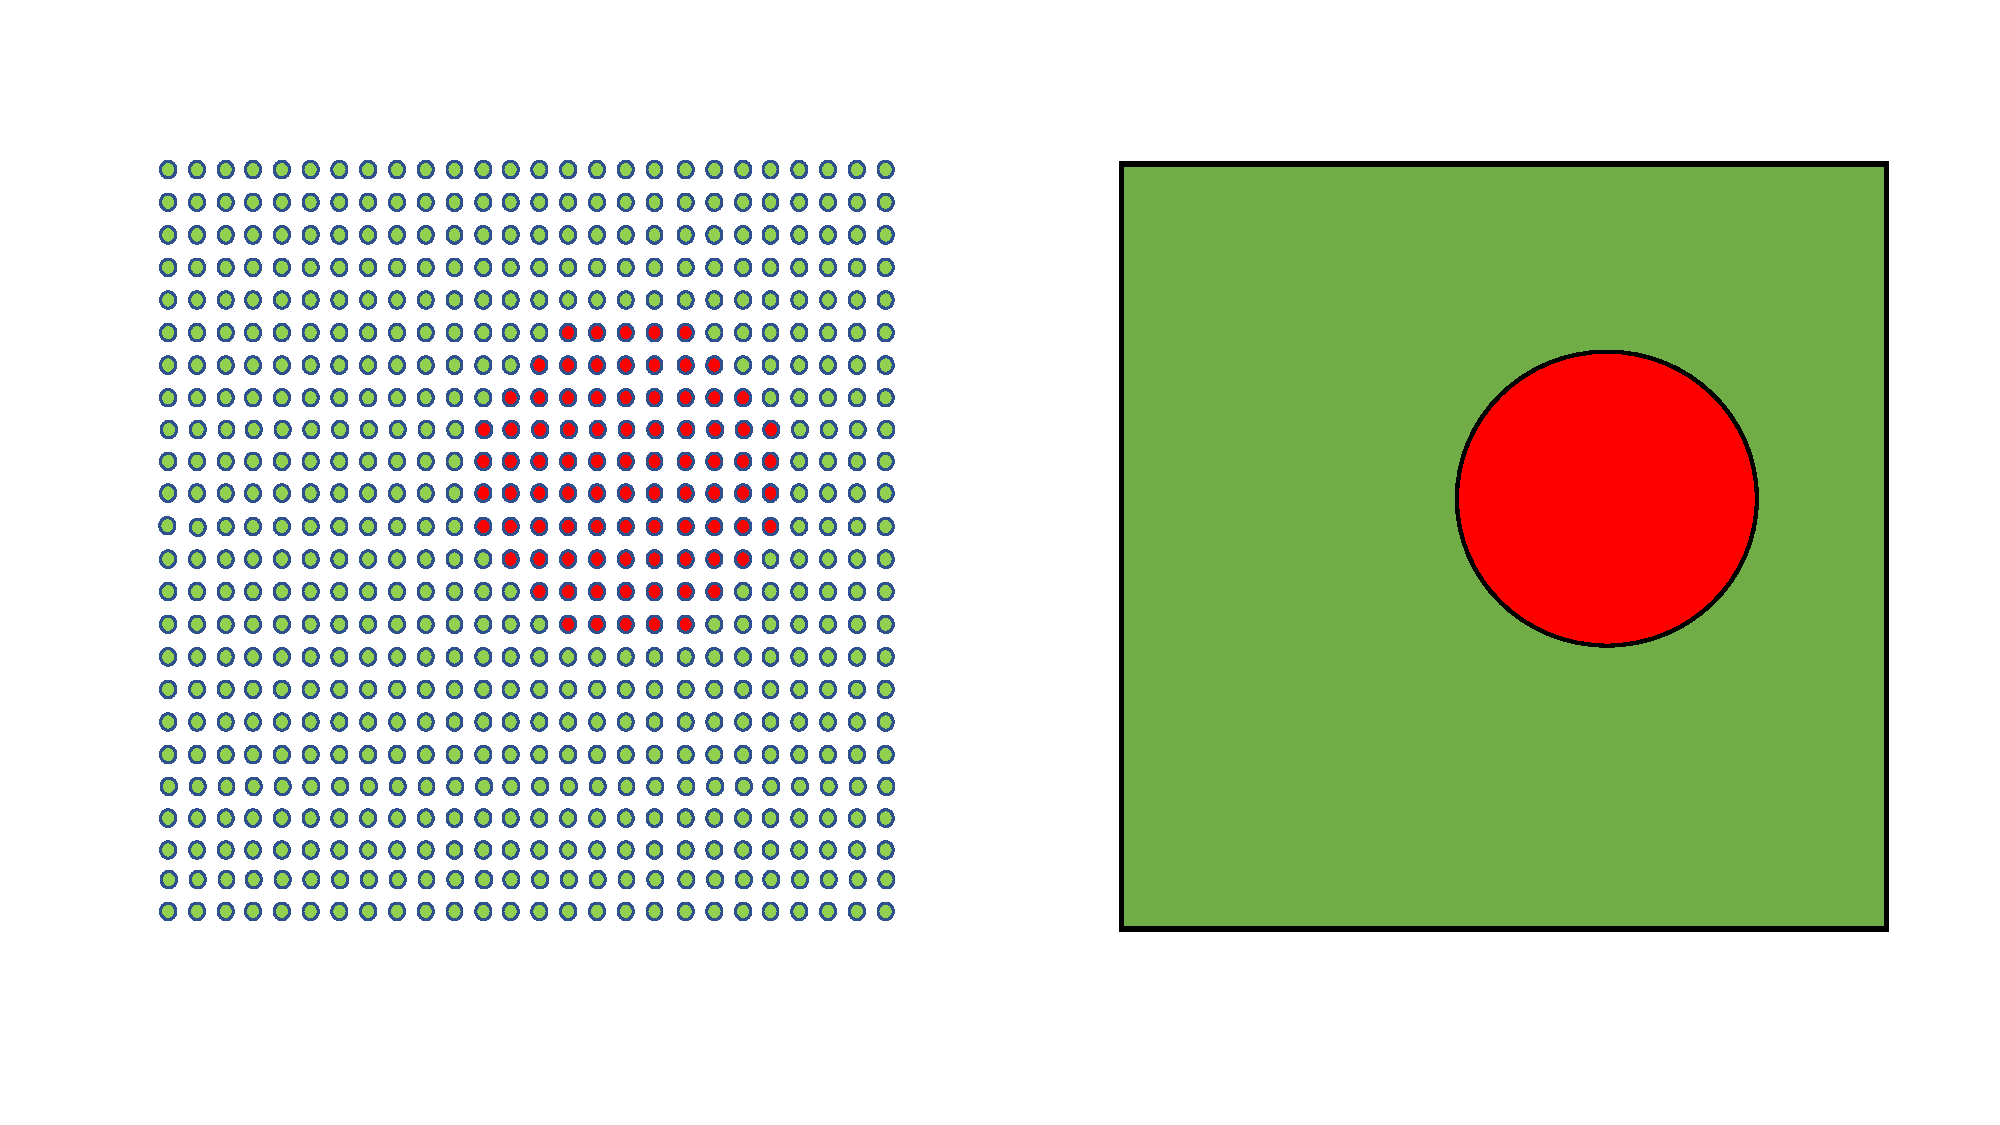
\includegraphics[width=0.7\linewidth]{discreteEntanglement.pdf}
	\caption{左は2次元格子系を表しており、ヒルベルト空間は赤と緑の領域に分解されている。この格子系の``連続極限"をとることで右の連続系でのヒルベルト空間の分解が得られる。}
	\label{fig:discreteentanglement}
\end{figure}

しかし実際に格子理論の領域を$A,B$の2つに分解して、その``連続極限"をとって連続理論へ持っていったときに、連続理論でのヒルベルト空間$\HH_A,\HH_B$やあるいは$A,B$上の局所演算子のなす作用素環$\mathfrak{A}_A,\mathfrak{A}_B$がどのようなものかを具体的に求めることは一般には容易ではない。さらに全系のヒルベルト空間$\HH$ないし局所演算子の作用素環$\mathfrak{A}$を$A,B$のテンソル積で分解できるかどうかも自明ではない。例えばゲージ理論では、$2$つの部分系に分解したときに超選択則による不定性が生じ、格子ゲージ理論ですらエンタングルメントを定義することが難しい\cite{Radicevic:2014kqa}\cite{Casini:2013rba}\cite{Aoki_2017}。こうした連続理論におけるエンタングルメントの問題に対して、代数的(公理論的)場の量子論の立場からアプローチする研究が最近盛んになされている\cite{hollands2018entanglement}\cite{Witten_2018}。

\section{Unruh効果}\label{sec:unruh}
ここでは場の量子論の真空のもつエンタングルメントから生じる現象であるUnruh効果について解説する。Unruh効果はブラックホールのHawking放射のトイモデルとして知られている。また、Unruh効果は代数的(公理論的)場の量子論によって導出できることが知られており、代数的(公理論的)場の量子論の立場からのエンタングルメントへのアプローチの指導原理の一つとなっている。

\subsub{$2$次元共形平坦空間での零質量自由スカラー場の正準量子化}
$1+1$次元Minkowski空間上の零質量自由スカラー場を、$ds^2=-dt^2+dx^2=e^{F(t_c,x_c)}(-dt_c^2+dx_c^2)$となる共形平坦座標$(t_c,x_c),\ (-\infty<t_c<\infty,-\infty<x_c<\infty)$において正準量子化することを考える。Minkowski空間の平坦座標$(t,x)$も自明に共形平坦であり、$(t_c,x_c)$での正準量子化はMinkowski空間の場合とまったく同様に行われる。

いま光円錐座標$x_c^\pm=x_c\pm t_c,\del_{c,\pm}=\frac{1}{2}(\del_{x_c}\pm \del_{t_c})$を導入すれば$ds^2=e^{F(x_c^-,x_c^+)}dx_c^-dx_c^+$で、零質量自由スカラー場の作用は共形不変なので、
\begin{align}
S[X]&=\int d^2 x\sqrt{-\det g} \left(-\frac{1}{2}g^{\mu\nu}\del_\mu X \del_\nu X\right)\notag\\
&=-\frac{1}{2}\int d^2x_c \left( -(\del_{t_c}X)^2+(\del_{x_c}X)^2 \right)\\
&=-\int dx_c^-dx_c^+(\del_{c,-} X \del_{c,+} X)
\end{align}
となる。とくに運動方程式は共形平坦座標においても波動方程式$\del_{c,-}\del_{c,+} X=0$になる。したがって運動方程式の解の完全系として、共形平坦座標での正エネルギーの平面波$e^{ip x_c^-}/\sqrt{2\pi\times 2p}$をとると、正エネルギー解$X$は
\begin{align}
X(x_c^-)=\int_{0}^{\infty} \frac{dp}{\sqrt{4\pi p}} (a_p^{c}e^{ip x_c^-}+a_p^{c\dagger}e^{-ip x_c^-})
\end{align}
と平面波展開できる。また、共形平坦座標におけるハミルトニアン$H_c$は
\begin{align}
H_c=\int_0^\infty dp\  p a_p^{c\dagger} a_p^c
\end{align}
とモード展開できる。

正準同時交換関係を課して$X$を正準量子化すれば、$a_p^{c\dagger},a_p^c$は生成消滅演算子と解釈でき、交換関係
\begin{align}
[a_p^c,a_q^c]=0=[a_p^{c,\dagger},a_q^{c,\dagger}],\quad [a_p^c,a_q^{c,\dagger}]=\delta(p-q)
\end{align}
を満たす。このとき共形平坦座標でのFock真空は$a_p^c|0\ra_c=0$で定義される。

いま$x_c^-$の複素数値関数$f,g$に対してKlein-Gordon双線形形式$(\ ,\ )$を
\begin{align}
(f,g)=-i\int_{-\infty}^\infty dx_c^-  (\overline{f}\del_{c,-}g-(\del_{c,-}\overline{f})g)
\end{align}
で定める。定義より$(f,g)=\overline{(g,f)}$が成り立つことに注意しておく。

正エネルギーの平面波$X_p^c=e^{ip x_c^-}/\sqrt{4\pi p},\ \overline{X_p^c}=e^{-ip x_c^-}/\sqrt{4\pi p}$は、Klein-Gordon双線形形式に対して直交系となす。すなわち$p,q>0$より、
\begin{align}
(X_p^c,X_q^c)&=\delta(p-q)\\ (X_p^c,\overline{X_q^c})&\propto \delta(p+q)=0
\end{align}
となる。

\subsub{Unruh効果}
$1+1$次元Minkowski空間$ds^2=-dt^2+dx^2$の局所座標として、Rindler座標$(t_L,x_L),(t_R,t_R)$を
\begin{align}
t&=\mp a^{-1}e^{ax_{L,R}} \sinh at_{L,R}\\
x&=\mp a^{-1}e^{ax_{L,R}} \cosh at_{L,R}
\end{align}
で定義する。この座標は左右の\textbf{Rindler wedge} $W_L,W_R$上で定義された座標であり、$W_L$と$W_R$は因果的に独立な領域になっている(図\ref{fig:rindlerwedge})。
\begin{align}
W_{L,R}=\{(t,x)\mid x^2>t^2, \mp x>0 \}
\end{align}
\begin{figure}[h]
	\centering
	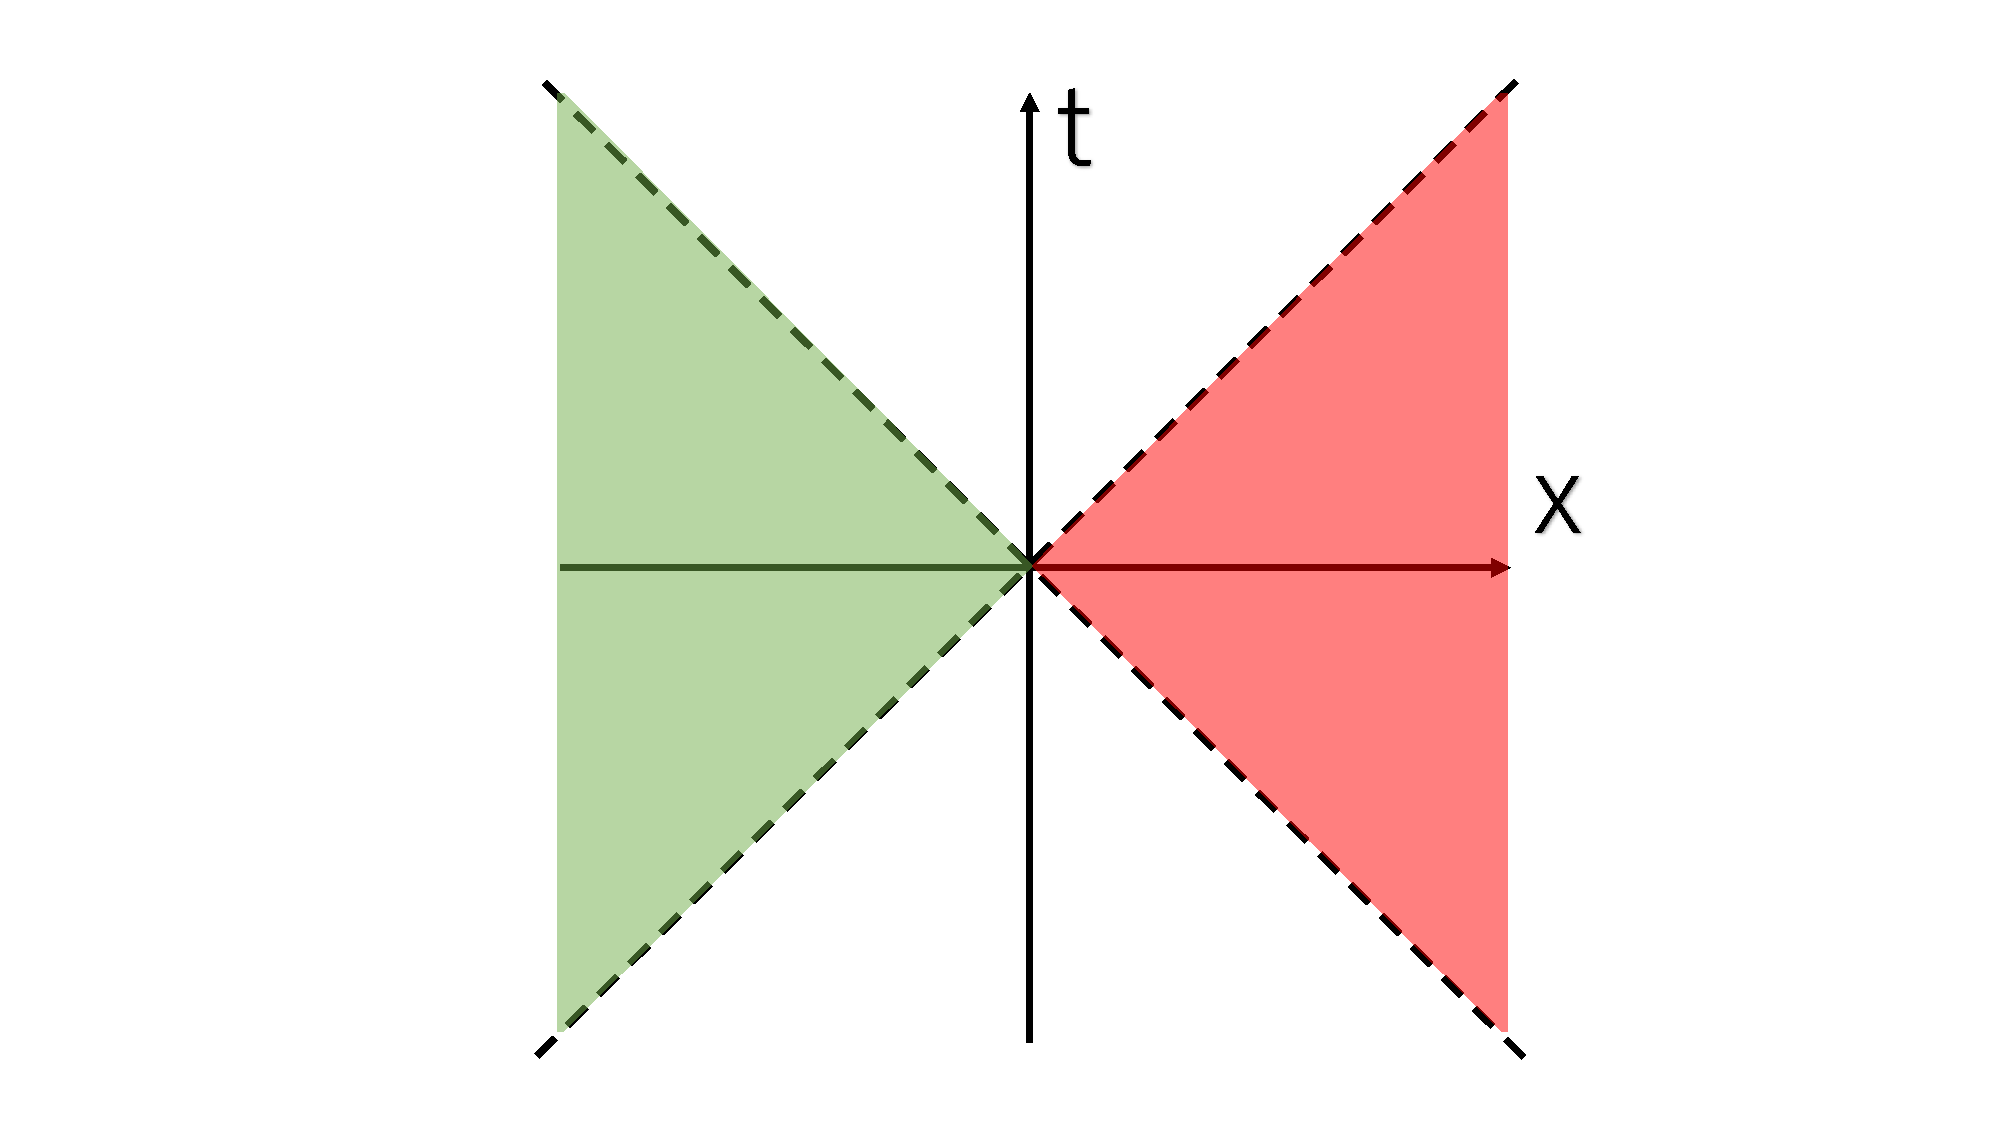
\includegraphics[width=0.7\linewidth]{rindlerwedge.pdf}
	\caption{Minkowski空間に埋め込んだRindler wedgeの図。赤・緑の領域がそれぞれRindler wedge $W_R,W_L$を表している。}
	\label{fig:rindlerwedge}
\end{figure}


計量は$ds^2=e^{2ax_{L,R}}(-dt_{L,R}^2+dx_{L,R}^2)$であるから、$(t_L,x_L),(t_R,t_R)$は共形平坦座標である。時間的Killingベクトル$\del_{t_{L,R}}=a(x\del_t+t\del_x)$に対応するハミルトニアン$K_{L,R}$はLorentzブーストの生成子に他ならず、
\begin{oframed}
\begin{align}
K_{L,R}=\int_{\mp x>0} xT_{00}(t,x) dx\label{modham}
\end{align}
\end{oframed}
と定義する。$K_{L,R}$は$W_{L,R}$の\textbf{モジュラーハミルトニアン(modular Hamiltonian)}とも呼ばれる。

スカラー場$X$の正エネルギー平面波での展開を、Minkowski座標と左右のRindler wedgeの2つで行うと
\begin{align}
X&=\int_{0}^{\infty}\frac{dp}{\sqrt{4\pi p}}(a_p e^{ip x^-}+a_p^{\dagger}e^{-ip x^-})\\
&=\int_{0}^{\infty} \frac{dp}{\sqrt{4\pi p}}(a_p^{L}e^{ip x_L^-}+a_p^{L\dagger}e^{-ip x_L^-}+a_p^{R}e^{ip x_R^-}+a_p^{R\dagger}e^{-ip x_R^-})
\end{align}
と展開され、正準交換関係は
\begin{align}
[a_p,a_q^\dagger]=[a_p^{L},a_q^{L,\dagger}]=[a_p^{R},a_q^{R,\dagger}]=\delta(p-q),\quad  (\text{otherwise})=0
\end{align}
となっている。生成消滅演算子を用いれば、モジュラーハミルトニアンは
\begin{align}
K_{L,R}=\int_{0}^{\infty} dp\  p a_p^{L,R\dagger}a_p^{L,R}
\end{align}
と展開できる。

いま平面波がKlein-Gordon双線形形式に対して直交系になることから、
\begin{align}
a_p=(X_p,X)=\int_{0}^{\infty}dq(a_q^{L}(X_p,X_q^L)+a_p^{L\dagger}(X_p,\overline{X_q^L})+a_p^{R}(X_p,X_q^R)+a_p^{R\dagger}(X_p,\overline{X_q^R}))
\end{align}
と展開できる。Minkowski座標とRindler座標の光円錐座標$x^\pm, x_{L,R}^\pm$は
\begin{align}
x^\pm=-a^{-1}e^{ax_L^\pm}=a^{-1}e^{ax_R^\pm}
\end{align}
で関係づいていることに注意すれば、$X_q^{L,R}=\theta(\mp x^-)\times (\mp ax^-)^{iq/a} /\sqrt{4\pi q}$と書ける。ただし$\theta(x)$は$x>0$で$1$、$x<0$で$0$となるHeaviside関数を表している。

これを用いて展開係数を計算すると
\begin{align}
(X_p,X_q^L)&=\frac{1}{2\pi a}\sqrt{\frac{q}{p}}\left(\frac{a}{p}\right)^{\dfrac{-iq}{a}}\exp\left(\frac{\pi q}{2a}\right)\Gamma\left(\frac{-iq}{a}\right)\\
(X_p,\overline{X_q^L})&=-\frac{1}{2\pi a}\sqrt{\frac{q}{p}}\left(\frac{a}{p}\right)^{\dfrac{iq}{a}}\exp\left(-\frac{\pi q}{2a}\right)\Gamma\left(\frac{iq}{a}\right)\\
(X_p,X_q^R)&=\frac{1}{2\pi a}\sqrt{\frac{q}{p}}\left(\frac{a}{p}\right)^{\dfrac{iq}{a}}\exp\left(\frac{\pi q}{2a}\right)\Gamma\left(\frac{iq}{a}\right)\\
(X_p,\overline{X_q^R})&=-\frac{1}{2\pi a}\sqrt{\frac{q}{p}}\left(\frac{a}{p}\right)^{\dfrac{-iq}{a}}\exp\left(-\frac{\pi q}{2a}\right)\Gamma\left(\frac{-iq}{a}\right)
\end{align}
となり、さらにこれらは
\begin{align}
\int_{0}^{\infty}dq (X_p^R,X_q)(X_q,X_{p'}^L)&=0\\
\int_{0}^{\infty}dq (X_p^R,X_q)(X_q,\overline{X_{p'}^L})&=-\frac{e^{\pi p/a}}{e^{2\pi p/a}-1}\delta(p-p')\\
\int_{0}^{\infty}dq (X_p^R,X_q)(X_q,X_{p'}^R)&=\frac{e^{2\pi p/a}}{e^{2\pi p/a}-1}\delta(p-p')\\
\int_{0}^{\infty}dq (X_p^R,X_q)(X_q,\overline{X_{p'}^R})&=0
\end{align}
を満たしている。$X_p^L$についても同様の式が成り立つ。

したがってMinkowski座標での真空の定義$a_p|0\ra_M=0$から、
\begin{align}
0&=\int_{0}^{\infty} dp (X_q^R,X_p)a_p|0\ra_M=(1-e^{-2\pi q/a})^{-1}(a_q^R-e^{-\pi q/a}a_q^{L\dagger})|0\ra_M\\
&=\int_{0}^{\infty} dp (X_q^L,X_p)a_p|0\ra_M=(1-e^{-2\pi q/a})^{-1}(a_q^L-e^{-\pi q/a}a_q^{R\dagger})|0\ra_M
\end{align}
となるから、Minkowski座標の真空$|0\ra_M$と左右のRindler座標の真空$|0\ra_L,|0\ra_R$は
\begin{align}
|0\ra_M &\propto \exp\left(\int_0^\infty dp\  e^{-\pi p/a}a_p^{L\dagger}a_p^{R\dagger} \right)|0\ra_L\tensor |0\ra_R\\
&=\sum_{n=0}^{\infty}\frac{1}{n!}\int_{p_i>0} dp_1\cdots dp_n e^{-\pi (p_1+\cdots+p_n)/a}a_{p_1}^{L\dagger}\cdots a_{p_n}^{L\dagger}|0\ra_L\tensor a_{p_1}^{R\dagger}\cdots a_{p_n}^{R\dagger}|0\ra_R
\end{align}
と関係していることが分かる。これはthemofield double状態になっていて、実際
\begin{oframed}
\begin{align}
\tr_L|0\ra\la0|_M&\propto\sum_{n=0}^{\infty}\frac{1}{n!}\int_{p_i>0} dp_1\cdots dp_n e^{-2\pi (p_1+\cdots+p_n)/a}a_{p_1}^{R\dagger}\cdots a_{p_n}^{R\dagger}|0\ra_R\la 0|_R a_{p_1}^{R}\cdots a_{p_n}^{R}\\
&=e^{-2\pi a^{-1}K_R}
\end{align}
\end{oframed}
となる。したがってMinkowski空間の真空を右側のRindler空間$W_R$で見ると、逆温度$\beta=2\pi/a$のカノニカル分布に見えることが分かる。この効果を\textbf{Unruh効果(Unruh effect)}\cite{Unruh1976}という。ブラックホールのHawking放射もこれと同様の現象として説明できる。

Unruh効果は、Wightmanの公理系を課した代数的場の量子論の枠組みから導出することもでき、Bisognano-Wichmannの定理\cite{bisognano1975duality}として知られている。これついては\cite{Araki2001}\cite{haag2012local}に詳しい解説が載っている。

\section{エンタングルメントエントロピー}\label{sec:EE}
ここでは純粋状態のエンタングルメントを測る唯一の量であるエンタングルメントエントロピーについて解説する。そして場の量子論の状態のエンタングルメントエントロピーの計算方法であるレプリカ法も説明する。

\subsection{エンタングルメントエントロピーの定義}
\subsub{von Neumannエントロピー}
複素ヒルベルト空間$\HH$上の状態$\rho$の\textbf{(von Neumann)エントロピー}$S(\rho)$を
\begin{oframed}
\begin{align}
S(\rho)=-\tr \rho\log\rho
\end{align}
\end{oframed}
で定める。ただし$-0\log 0=0$としている。

von Neumannエントロピーは正値$S(\rho)\geq 0$で、等号成立は純粋状態のときのみである。また、von Neumannエントロピーはユニタリー変換$U$に対して不変$S(U^\dagger \rho U)=S(\rho)$で、ユニタリーな時間発展で変化しない。

\begin{ex}
カノニカル分布$\rho_\beta=e^{-\beta H}/Z(\beta)$のvon Neumannエントロピーは
\begin{align}
S(\rho_\beta)&=-\tr (e^{-\beta H}/Z(\beta))\log(e^{-\beta H}/Z(\beta))\notag\\
&=\beta \la H\ra_{\rho_\beta}+\log Z(\beta)\notag\\
&=\beta (\la H\ra_{\rho_\beta}-F(\beta))
\end{align}
となる。ただし$\la H\ra_{\rho}=\tr \rho H$は状態$\rho$でのエネルギーの期待値であり、また、$F(\rho)=-\beta^{-1}\log Z(\beta)$はHelmholtz自由エネルギーである。
\end{ex}

\begin{oframed}
合成系$\HH=\HH_A\tensor \HH_B$の状態$\rho$に対して、$B,A$系をトレースアウトしてできる$A,B$系の密度行列を$\rho_A=\tr_B \rho,\ \rho_B=\tr_A \rho$として、$A$の\textbf{エンタングルメントエントロピー(entanglement entropy)}を$S(\rho_A)$で定める。
\end{oframed}

$\rho$が純粋状態なら$S(\rho_A)=S(\rho_B)$となる。実際、$\rho=|\Psi\ra\la\Psi|$で決まるベクトル$\Psi$をSchmit展開すれば
\begin{align}
\Psi=\sum_{i} d_i |\psi_A^i\ra\tensor |\psi_B^i\ra,\ \rho=\sum_{i} d_i^2 |\psi_A^i\ra\la\psi_A^i|\tensor |\psi_B^i\ra\la\psi_B^i|
\end{align}
であり、$\rho_{A}=\sum_{i} d_i^2 |\psi_{A}^i\ra\la\psi_{A}^i|,\rho_{B}=\sum_{i} d_i^2 |\psi_{B}^i\ra\la\psi_{B}^i|$となるので
\begin{align}
S(\rho_A)=-\sum_{i} d_i^2 \log(d_i^2)=S(\rho_B)
\end{align}
が分かる。したがって純粋状態に対しては、部分系への分解の仕方のみでエンタングルメントエントロピーが決まる。$\HH$の混合状態に対しては$S(\rho_A)=S(\rho_B)$が成り立つとは限らない。純粋状態がセパラブルならエンタングルメントエントロピーは$0$であり、エンタングルメントエントロピーは純粋状態のエンタングルメントの強さを測る唯一の量になっている。

例\ref{tfdpartialtrace}より、thermofield double状態のエンタングルメントエントロピーはカノニカル分布のvon Neumannエントロピーに等しい。
\begin{ex}
2次元Minkowski空間上の$t=0$面に零質量自由スカラー場の真空$|0\ra\la 0|_M$を用意する。このときRindler wedge $W_R$のエンタングルメントエントロピーは
\begin{align}
S(\rho_R)&=S(\tr_L |0\ra\la 0|_M)=S(e^{-2\pi a^{-1}K_R}/Z)=2\pi a^{-1}\la K_R \ra_{\rho_R}+\log Z
\end{align}
となる。一般に、場の量子論を2つの空間領域に分解したとき、エンタングルメントエントロピーは真空でさえ0ではなく、しかも紫外発散を含む量になっている。
\end{ex}


\subsub{von Neumannエントロピーの特徴づけ}
複素ヒルベルト空間$\HH$上の密度行列全体の空間$T(\HH)_{1+}$から$[0,\infty]$への写像$\Theta\colon T(\HH)_{1+}\to[0,\infty]$であり、以下の7つの性質を満たすものは定数倍を除いてvon Neumannエントロピ$S$に一致することが知られている。

\begin{enumerate}
\item $\Theta$はユニタリー不変
\begin{align}
\forall U\text{;ユニタリー},\ \Theta(U^\dagger \rho U)=\Theta(\rho)
\end{align}
\item 直和空間$\directsum_{k=1}^n \HH_k$の上の、直和で表される状態$\directsum_{k=1}^n a_k\rho_k,\ \sum_{k}a_k=1$に対して
\begin{align}
\Theta(\directsum_{k=1}^n a_k\rho_k)=\sum_{k=1}^{n}a_k\Theta(\rho_k)+\Theta\left( \text{diag}(a_1,\cdots,a_n) \right)
\end{align}
\item テンソル積空間$\tensor_{k=1}^n \HH_k$の上の、テンソル積で表される状態$\tensor_{k=1}^n \rho_k$に対して、次の\textbf{加法性(additivity)}を満たす。
\begin{align}
\Theta(\tensor_{k=1}^n \rho_k)=\sum_{k=1}^{n}\Theta(\rho_k)
\end{align}
\item テンソル積空間$\HH_1\tensor\HH_2$上の密度行列$\rho_{12}$に対して$\rho_1=\tr_2 \rho_{12},\ \rho_2=\tr_1 \rho_{12}$と書くとき、次の\textbf{劣加法性(subadditivity)}を満たす。
\begin{align}
\Theta(\rho_{12})\leq \Theta(\rho_1)+\Theta(\rho_2)
\end{align}
\item $\dim_\C\HH=1$なら$\Theta(\forall\rho)=0$
\item $\dim_\C\HH<\infty$なら$\Theta(\forall\rho)<\infty$で、$\Theta$は$\rho$の固有値についての連続関数
\item $\dim_\C\HH=\infty$のとき、階数が有限でない密度行列を$\rho=\sum_{n=1}^{\infty} \lambda_n P_n,\ (\lambda_1\geq \lambda_2\geq\cdots\text{かつ}\\n\to \infty\text{で}\lambda_n\to 0)$とスペクトル分解する。このスペクトルにカットオフを入れて定めた$\rho_N=\sum_{n=1}^{N}\lambda_n P_n/\sum_{n=1}^{N}\lambda_n$を定義すると
\begin{align}
\Theta(\rho_N)\to \Theta(\rho)\  (N\to \infty)
\end{align}
と収束する。
\end{enumerate}

\hfill\newline

von Neumannエントロピー(あるいはエンタングルメントエントロピー)はまた、次の不等式を満たすことも知られている。

\textbf{荒木-Lieb不等式}
\begin{align}
|S(\rho_1)-S(\rho_2)|\leq S(\rho_{12})
\end{align}

\textbf{強劣加法性(strong subadditivity)}
\begin{align}
S(\rho_{123})+S(\rho_2)&\leq S(\rho_{12})+S(\rho_{23})\\
S(\rho_{1})+S(\rho_2)&\leq S(\rho_{13})+S(\rho_{23})\label{ssa}
\end{align}

\subsub{Renyiエントロピー}
$\alpha\in(0,1)\union (1,\infty)$に対して、密度行列$\rho$の\textbf{$\alpha-$Renyiエントロピー}を
\begin{oframed}
\begin{align}
S_\alpha(\rho)=\frac{1}{1-\alpha}\log \tr \rho^\alpha
\end{align}
\end{oframed}
で定める。$S(\rho)=\lim_{\alpha\to 1}S_\alpha (\rho)=-\lim_{\alpha\to 1}\del_{\alpha} \log \tr \rho^\alpha$となっている。

\subsection{相対エントロピーとBekenstein bound}
複素ヒルベルト空間$\HH$上の$2$つの状態$\rho,\sigma$の\textbf{相対エントロピー(relative entropy)}$S(\rho||\sigma)$を
\begin{oframed}
\begin{align}
S(\rho||\sigma)=\tr \rho\log(\rho-\sigma)
\end{align}
\end{oframed}
で定める。相対エントロピーは正値$S(\rho||\sigma)\geq 0$で、等号成立は$\rho=\sigma$のときのみである。また、相対エントロピーはユニタリー変換$U$に対して不変$S(U^\dagger\rho U||U^\dagger \sigma U)=S(\rho||\sigma)$で、ユニタリーな時間発展で変化しない。

相対エントロピーはCPTP写像$\Lambda\colon B(\HH)\to B(\HH)$に対して、単調性$S(\Lambda^\ast \rho||\Lambda^\ast \sigma)\leq S(\rho||\sigma)$を満たす。
\begin{ex}
	ある状態$\rho$と逆温度のカノニカル分布$\rho_\beta$の相対エントロピー$S(\rho||\rho_\beta)$は
	\begin{align}
	S(\rho||\rho_\beta)&=\tr \rho\log(\rho-\rho_\beta)\notag\\
	&=-S(\rho)+\beta\la H\ra_{\rho}+\log Z(\beta)\\
	&=\beta(F(\rho)-F(\rho_\beta))
	\end{align}
	と、Helmholtz自由エネルギーの差になる。
\end{ex}

\subsub{CasiniによるBekenstein boundの導出}
ここで、Casini\cite{Casini:2008cr}によるBekenstein boundの導出を紹介する。\textbf{Bekenstein bound}\cite{Bekenstein:1980jp}とは一般的な物理系のもつエントロピーの普遍的な上限を示唆する式のことで、
\begin{align}
S\le O(1)RE
\end{align}
という式である。ただし$S,R,E$は系のエントロピー、典型的な半径、エネルギーを表している。Bekensteinはもともと、ブラックホールに小さな物体を入れた時にブラックホール熱力学の一般化された第二法則を考えて、この不等式を導出した。これに対してCasiniは相対エントロピーを用いて、この不等式を非常に一般的な設定のもとで導出した。

Minkowski空間の零質量自由スカラー場の真空をRindler wedge $W_R$にトレースアウトした密度行列を、モジュラーハミルトニアン$K_R$を用いて$\rho_{\text{vac},R}=e^{-\beta K_R}$と書く。このとき相対エントロピーの正値性から、$W_R$上の任意の密度行列$\rho_R$に対して
\begin{align}\label{bekensteinboundproof}
S(\rho_R)-S(\rho_{\text{vac},R})&=-S(\rho_R||\rho_{\text{vac},R})+\beta(\la K_R \ra_{\rho_R}-\la K_R\ra_{\rho_{\text{vac},R}})\notag\\
&\leq \beta(\la K_R \ra_{\rho_R}-\la K_R\ra_{\rho_{\text{vac},R}})
\end{align}
となる。

モジュラーハミルトニアンはLorentzブーストの生成子であり、\ref{modham}式から$K_A\sim (W_R\text{の``半径''})\times (W_R\text{でのエネルギー期待値})$と評価できる。したがって\ref{bekensteinboundproof}式は、Bekenstein bound $S\leq O(1)\times RE$を与えている。

\subsection{レプリカ法}
$d$次元Minkowski時空上の場の理論をWick回転してEuclid計量にして、$t\to \pm \infty$で系は真空状態にあるという境界条件を置く。$t=\pm \infty$からの経路積分で$t=0$に経路積分によって純粋状態$\rho=|\Psi\ra\la \Psi|$を用意する。

$t=0$の時間一定面での空間領域を$A,B$の$2$つに分けることで、エンタングルメントエントロピーを定義できる。このとき、$\rho$の部分トレースを経路積分として実行して
\begin{oframed}
\begin{align}
\rho_A=\tr_B\rho=\frac{1}{Z_{\R^d}}\int \mathcal{D}\psi_B(\vec{x}\in B)\ \la \psi_B|\Psi\ra\la \Psi|\psi_B\ra
\end{align}
\end{oframed}
とするのが\textbf{レプリカ法(replica trick)}である。

$A$が連結区間$[x_1,x_2]$で、$|\Psi\ra\la\Psi |$が真空状態なら、
\begin{align}
\tr_A \rho_A^n &= \frac{1}{Z^n} \tr_A \left(\int \mathcal{D}\psi_B(\vec{x}\in B)\la \psi_B|\Psi\ra\la |\Psi|\psi_B\ra\right)^n\\
&=\frac{Z_{(\R^d)^n}}{(Z_{\R^d})^n}
\end{align}
となる。ただし$\R^d$上の分配関数を$Z_{\R^d}$と書いた。また、$(\R^d)^n$は$A$を分岐とする$\R^d$の$n$重被覆のことで、$(\R^d)^n$上の分配関数を$Z_{(\R^d)^n}$と書いた。これを図に表すと図\ref{fig:replicatrick}のようになる。
\begin{figure}[h]
	\centering
	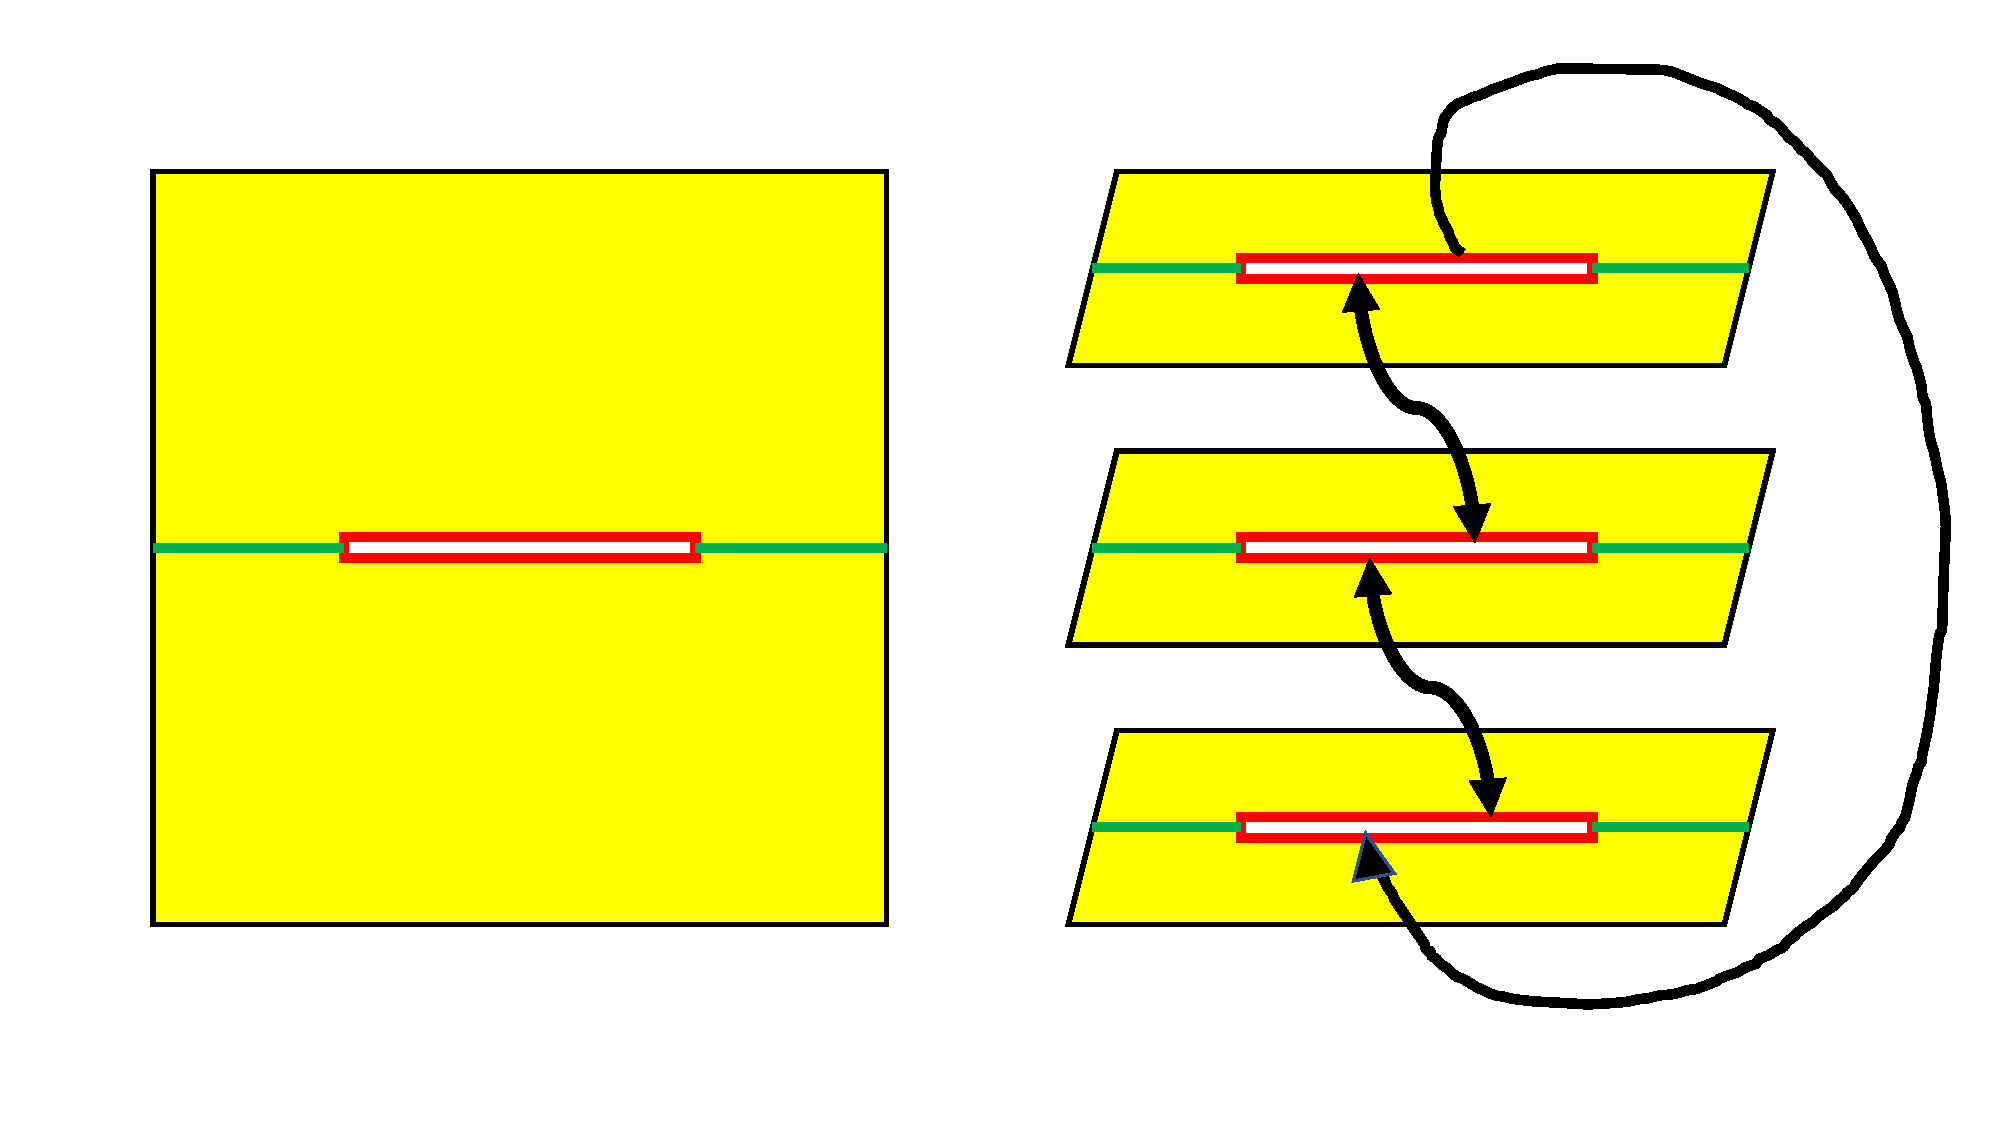
\includegraphics[width=0.7\linewidth]{replicatrick.pdf}
	\caption{左の$\tau=0$に用意された状態$\rho_A$を表している。これを$n=3$倍してトレースをとった$\tr_A\rho_A^3$を表した図が右である。}
	\label{fig:replicatrick}
\end{figure}

したがって真空をトレースアウトしてできた$A$系での混合状態の$n-$Renyiエントロピーは
\begin{align}
S_n(\rho_{A})=-\frac{1}{n-1}(\log Z_{(\R^d)^n} -n \log Z_{\R^d})
\end{align}
である。この$n$を実数へと解析接続して$n\to 1$の極限をとればエンタングルメントエントロピー$S(\rho_A)$が得られる。

\section{2次元共形場理論におけるエンタングルメントエントロピー}\label{sec:EEcft2}
ここでは前節で導入したレプリカ法を用いて、2次元共形場理論におけるエンタングルメントエントロピーを計算する。2次元共形場理論におけるエンタングルメントエントロピーは中心電荷と系の大きさのみで決まり、この結果は格子模型の数値計算によっても確認されている。以下では本研究での解析にも用いた、2次元零質量自由Dirac場の真空のエンタングルメントエントロピーの計算方法を解説し、そのあと一般の2次元共形場理論の真空のエンタングルメントエントロピーの計算方法を解説する。

\subsection{2次元零質量自由ディラック場でのエンタングルメントエントロピー}
\subsub{$A$が直線上の連結区間の場合}
平面$\C$上の2次元零質量自由ディラック場を考え、経路積分によって$\tau=0$の直線上に真空状態を用意する。このとき$\tau=0$の直線を2つの部分系$A,B$に分けてエンタングルメントを定義する。$A$が連結区間$[x_1,x_2]$の場合、レプリカ法を用いて真空$\rho=|0\ra\la 0|$に対して$\tr_A \rho_A^n$を計算するには、$\C$の$n$重orbifoldについての分配関数$Z_{(\C)^n}$を計算すればよい。

これを計算するために、場$\psi,\overline{\psi},\tilde{\psi},\overline{\tilde{\psi}}$をボソン化して得られるスカラー場$X$を用いて、\textbf{ツイスト演算子(twist operator)}
\begin{align}\label{twistopscalarplane}
\sigma_k(z,\overline{z})=e^{i\frac{k}{n}(X_L(z)-X_R(\overline{z}))}=V_{(k/n,-k/n)}(z,\overline{z})\quad \left(k=-\frac{n-1}{2},-\frac{n-3}{2},\cdots \frac{n-1}{2}\right)\\
\overline{\sigma}_k(z,\overline{z})=e^{-i\frac{k}{n}(X_L(z)-X_R(\overline{z}))}=V_{(-k/n,k/n)}(z,\overline{z})\quad \left(k=-\frac{n-1}{2},-\frac{n-3}{2},\cdots \frac{n-1}{2}\right)
\end{align}
を導入する。このとき、場$\psi,\overline{\psi},\tilde{\psi},\overline{\tilde{\psi}}$とツイスト演算子$\sigma,\overline{\sigma}$の演算子積展開は\ref{vertexopOPE}から
\begin{align}
\psi(z)\sigma_k(0,0)&\propto z^{k/n}\\
\tilde{\psi}(\overline{z})\sigma_k(0,0)&\propto \overline{z}^{-k/n}\\
\overline{\psi}(z)\overline{\sigma}_k(0,0)&\propto z^{k/n}\\
\overline{\tilde{\psi}}(\overline{z})\overline{\sigma}_k(0,0)&\propto \overline{z}^{-k/n}
\end{align}
となる。したがって例えば場$\psi$を$z\to e^{2\pi i}z$とツイスト演算子の周りに半時計周りに1周させたときに、$\psi$は位相$e^{2\pi ik/n}$を獲得する。

よって平面$\C$を$n$重にoribifoldした空間での零質量自由Dirac場での相関関数は、平面$\C$にツイスト演算子を挿入した相関関数に等しい。したがって分配関数$Z_{(\C)^n}$は
\begin{align}
\tr_A \rho_A^n&=\frac{Z_{(\C)^n}}{(Z_{\C})^n}\\
&=\prod_{k=0}^{n-1} \la \sigma_k(x_1)\overline{\sigma}_k(x_2) \ra_{\C}\\
&\propto \prod_{k=0}^{n-1}\frac{1}{(x_1-x_2)^{2(h_k+\overline{h}_k)}}
\end{align}
と計算できる。ただし$h_k=\overline{h}_k=k^2/2n^2$である。

$n$が奇数・偶数どちらであっても
\begin{align}
\sum_{k=-(n-1)/2}^{(n-1)/2} \frac{k^2}{n^2} =\frac{1}{12}\left(n-\frac{1}{n}\right)
\end{align}
となる。したがって$\tr_A \rho_A^n \propto (x_1-x_2)^{\frac{1}{6}(n-1/n)}$を得るので、
\begin{align}\label{freediracEEplane}
S(\rho_{A})=\frac{1}{3}\log \frac{|x_1-x_2|}{\epsilon}
\end{align}
となる。ただしここで紫外発散のカットオフパラメーター$\epsilon$を導入した。

\subsub{$A$が円筒上の連結区間の場合}
空間方向が半径$L$の円周にコンパクト化された2次元零質量自由ディラック場の真空のエンタングルメントエントロピーは同様に、$\la \sigma_k(x_1)\overline{\sigma}_k(x_2)\ra_{S_L^1\times \R}$を計算すればよく、
\begin{align}
S(\rho_{A})=\frac{1}{3}\log \left(\frac{2L}{\epsilon}\sin\left(\frac{x_1-x_2}{2L}\right)\right)
\end{align}
となる。

また、直線上の温度$2\pi\beta$のカノニカル分布のエンタングルメントエントロピーは、上のセットアップの座標を$i$倍して、$L$を$\beta$に読み替えればいいので、
\begin{align}
S(\rho_{A})=\frac{1}{3}\log \left(\frac{2\beta}{\epsilon}\sinh\left(\frac{x_1-x_2}{2\beta}\right)\right)
\end{align}
となる。とくに$\beta\to 0$の高温極限($\iff |x_1-x_2|\gg 1$の熱力学極限)をとると、
\begin{align}
S(\rho_{A})\sim\frac{1}{3}\log\frac{2\beta}{\epsilon}+\frac{1}{6}\frac{|x_1-x_2|}{\beta}
\end{align}
となり、第$2$項は通常の熱力学的な示量的エントロピーになっている。

\subsub{$A$が直線上の非連結区間の場合}
平面$\C$の$\tau=0$の直線上の真空について、$N$個の連結成分をもつ区間とそれ以外とのエンタングルメントエントロピーをレプリカ法で計算すると、$n$重にorbifoldされた空間の被覆空間は$g=(n-1)(N-1)$の種数をもったコンパクトRiemann面となる。

とくに$N=2$で$A=[x_1,x_2]\union [x_3,x_4]\ (x_1<x_2<x_3<x_4)$のとき、零質量自由Dirac場でのエンタングルメントエントロピーをレプリカ法で計算すると、各$n$に対して種数$n-1$のコンパクトRiemann面に対する相関関数を計算することになる。したがって$n\geq 2$では、相関関数はモジュライ空間のパラメータの不定性が生じる。しかし最終的に$n\to 1$の極限をとるので、エンタングルメントエントロピーを計算する上ではモジュライパラメータは関係せず、平面上のツイスト演算子$\sigma(x_1)\overline{\sigma}(x_2)\sigma(x_3)\overline{\sigma}(x_4)$の相関関数を計算すればよい。したがって零質量自由Dirac場での$A$のエンタングルメントエントロピーは
\begin{align}
S(\rho_A)=\frac{1}{3}\log\frac{|x_1-x_2||x_3-x_4||x_1-x_4||x_2-x_3|}{\epsilon^2|x_1-x_3||x_2-x_4|}
\end{align}
となる。

\subsection{一般の2次元共形場理論でのエンタングルメントエントロピー}
\subsub{$A$が直線上の連結区間の場合}
平面$\C$上の2次元共形場理論を考え、経路積分によって$\tau=0$の直線上に真空状態を用意する。このとき$\tau=0$の直線を2つの部分系$A,B$に分けてエンタングルメントを定義する。$A$が連結区間$[x_1,x_2]$の場合、レプリカ法を用いて真空$\rho$に対して$\tr_A \rho_A^n$を計算するには、$\C$の$n$重orbifoldについての分配関数$Z_{(\C)^n}$を計算すればよい。

中心電荷$c$をもつ2次元共形場理論で$A=[x_1,x_2]$のときのorbifoldを実現するツイスト演算子は、次のように決まる。

まず共形変換によって平面座標$w$を
\begin{align}
z=\left(\frac{w-x_1}{w-x_2}\right)^{1/n}
\end{align}
によってRiemann球面を$n$等分した領域$z$に移すと、orbifoldによって$z=0,\infty$の2点が特異点になることが分かる。したがってこれに対応して$w=x_1,x_2$にツイスト演算子$\sigma_n,\overline{\sigma}_n$を挿入してorbifoldに対応する位相を獲得させればよい。

共形変換$w\to z$でエネルギー運動量テンソルは非テンソル的な変換をして、$\la T \ra_{w}=0$より、
\begin{align}
\la T \ra_{z}/Z_{(\C)^n}=\frac{c}{24}(1-n^{-2})\frac{(x_2-x_1)^2}{(w-x_1)^2(w-x_2)^2}
\end{align}
となる。これが$w$平面にツイスト演算子$\sigma_n(x_1)\overline{\sigma}_n(x_2)$を挿入したものに等しいとして
\begin{align}
\frac{\la T(w)\sigma_n(x_1)\overline{\sigma}_n(x_2)\ra_{\C}}{\la \sigma_n(x_1)\overline{\sigma}_n(x_2) \ra_{\C}}&\equiv n\la T \ra_{z}/Z_{(\C)^n}\\
&=\frac{c}{24}(n-n^{-1})\frac{(x_2-x_1)^2}{(w-x_1)^2(w-x_2)^2}
\end{align}
とすればよい。

このとき$w\to x_1,x_2$と近づける極限で発散を評価することで$\sigma_n,\overline{\sigma}_n$はそれぞれ
\begin{align}
h=\overline{h}=\frac{c}{24}\left(n-\frac{1}{n}\right)
\end{align}
の共形ウェイトをもつプライマリー場として解釈できることが分かる。

したがって$tr_A \rho_A^n$は
\begin{align}
tr_A \rho_A^n&=\frac{Z_{(\C)^n}}{(Z_{\C})^n}\\
&=\la \sigma_n(x_1)\overline{\sigma}_n(x_2) \ra_{\C}\\
&\propto |x_1-x_2|^{\frac{c}{6}\left(n-1/n\right)}
\end{align}
となるので、エンタングルメントエントロピーは
\begin{oframed}
\begin{align}\label{2dcftplaneEE}
S(\rho_A)=\frac{c}{3}\log\frac{|x_1-x_2|}{\epsilon}
\end{align}
\end{oframed}
となる。平面上の2次元共形場理論での連結区間とそれ以外とのエンタングルメントエントロピーは作用に関わらず中心電荷$c$のみで決まることがわかる。これは、平面上の2次元共形場理論のプライマリー場$2$点関数が定数倍を除いて共形ウェイトのみによって決定できることから来る性質である。

この結果は2次元共形場理論の真空のエンタングルメントエントロピーについての最も基本的な結果であり、1994年にHolzhey,Larsen,Wilczek\cite{Holzhey_1994}によって計算された。

\subsub{$A$が円筒上の連結区間の場合}
空間方向が半径$L$の円周にコンパクト化された2次元共形場理論の真空のエンタングルメントエントロピーを考える。円筒は平面$\C-\{0\}$から共形変換
\begin{align}
w=\tan\left(\frac{\pi z}{L}\right)
\end{align}
によって移すことができるので、ツイスト演算子がプライマリー場であることから、
\begin{oframed}
\begin{align}\label{2dcftcylEE}
S(\rho_A)=\frac{c}{3}\log \left(\frac{2L}{\epsilon}\sin\left(\frac{x_1-x_2}{2L}\right)\right)
\end{align}
\end{oframed}
となる\cite{Calabrese:2004eu}。

同様に平面上の温度$2\pi\beta$のカノニカル分布のエンタングルメントエントロピーは、上の設定を$i$倍して
\begin{oframed}
\begin{align}\label{2dcftthermalEE}
S(\rho_{A})=\frac{c}{3}\log \left(\frac{2\beta}{\epsilon}\sinh\left(\frac{x_1-x_2}{2\beta}\right)\right)
\end{align}
\end{oframed}
となる。とくにとくに$\beta\to 0$の高温極限($\iff |x_1-x_2|\gg 1$の熱力学極限)をとると、
\begin{align}
S(\rho_{A})\sim\frac{c}{3}\log\frac{2\beta}{\epsilon}+\frac{c}{6}\frac{|x_1-x_2|}{\beta}
\end{align}
となり、第$2$項は通常の熱力学的な示量的エントロピーになっている。

\subsub{$A$が非連結区間の場合}
$A$が2つの連結成分からなる非連結区間$A=[x_1,x_2]\union [x_3,x_4]\ (x_1<x_2<x_3<x_4)$の場合、零質量自由Dirac場のときと同様に$n\to 1$の極限を考えることで平面の4点関数を計算すればいい。しかし一般の共形場理論では複比の部分の不定性を決定できず、一般には
\begin{align}
S(\rho_A)=\frac{c}{3}\log\frac{|x_1-x_2||x_3-x_4||x_1-x_4||x_2-x_3|}{\epsilon^2|x_1-x_3||x_2-x_4|}+(\text{複比から来る項})
\end{align}
という形になる。

\section{AdS$_3$/CFT$_2$対応についての笠-高柳公式}\label{sec:RTformula}
ここではAdS$_3$/CFT$_2$対応についての笠-高柳公式を解説する。この公式は、\ref{chap:adscftreview}章で解説したAdS$_3$/CFT$_2$対応を用いて、重力双対を持つような2次元共形場理論でのエンタングルメントエントロピーをAdS$_3$空間内の測地線の長さに関係づける公式である。後に見るように、笠-高柳公式はある意味でBekenstein-Hawking公式の拡張になっており、AdS/CFT対応やブラックホール物理と量子情報理論を関係づける公式としてさまざまな応用研究がなされている。

\subsection{笠-高柳公式}
\subsub{公式}
\textbf{笠-高柳公式(Ryu-Takayanagi formula)}は、重力双対をもつような2次元共形場理論での部分系$A$についてのエンタングルメントエントロピー$S_A$に対して、次の対応を主張する。
\begin{oframed}
\begin{align}
S_A = \min_{\substack{\del\gamma=\del A\\ \gamma\text{と}A\text{で作られるループは0にホモロガス}}} \frac{\text{length}(\gamma)}{4G}
\end{align}
\end{oframed}
ここで、$\gamma$は$A$の境界からAdS$_3$の内部へ伸びる曲線である。条件「$\del\gamma=\del A$」によって曲線$\gamma$と部分系$A$の境界が一致していることが要請されている。また、「min」をとることから曲線$\gamma$は測地線になることも要請される。また、2つ目の条件「$\gamma$と$A$で作られるループは0にホモロガス」はホモロジー条件(homology constraint)と呼ばれ、$\gamma$と$A$で作られるループが穴を囲まないことを要請している。

笠-高柳公式はLewkowycz,Maldacena\cite{Lewkowycz:2013nqa}によって証明された。本論文ではこの証明の紹介はしないが、以下で様々な場合で左辺と右辺をそれぞれ計算して、この式の意味を味わってみる。また、以下でも「平面/円筒上の共形場理論」と書いたとき、空間$x$方向が直線/円周となっている共形場理論を指すことにする。

\subsub{具体例1 : 平面上のCFTの真空での、連結区間Aのエンタングルメントエントロピー}
平面上の真空について、連結区間$A=[x_1,x_2]$に対して笠-高柳公式の両辺を計算する。左辺のエンタングルメントエントロピーは共形場理論の中心電荷$c$
にしか依らず、(\ref{2dcftplaneEE})より、
\begin{align}
LHS=S(\rho_A)=\frac{c}{3}\log\frac{|x_1-x_2|}{\epsilon}
\end{align}
となる。右辺の測地線は一意に決まり、(\ref{geodlengthPoincare})より、
\begin{align}
RHS=\frac{\text{length}(\gamma)}{4G}=\frac{R_A}{2G}\log\frac{|x_1-x_2|}{\epsilon}
\end{align}
となる。AdS$_3$/CFT$_2$対応から、Brown-Henneaux中心電荷$c_A=3R_A/2G$は、2次元共形場理論の中心電荷$c$に等しい。したがって、この場合確かに笠-高柳公式が成立することが分かる。

\subsub{具体例2 : 円筒上のCFTの真空での、連結区間Aのエンタングルメントエントロピー}
半径$L$の円筒上の真空について、連結区間$A=[x_1,x_2]$に対して笠-高柳公式の両辺を計算する。左辺のエンタングルメントエントロピーは共形場理論の中心電荷$c$
にしか依らず、(\ref{2dcftcylEE})より、
\begin{align}
LHS=S(\rho_A)=\frac{c}{3}\log \left(\frac{2L}{\epsilon}\sin\left(\frac{x_1-x_2}{2L}\right)\right)
\end{align}
となる。右辺の測地線は一意に決まり、(\ref{geodlengthGlobal})より、
\begin{align}
RHS=\frac{\text{length}(\gamma)}{4G}=\frac{R_A}{2G}\log \left(\frac{2L}{\epsilon}\sin\left(\frac{x_1-x_2}{2L}\right)\right)
\end{align}
となる。したがってAdS$_3$/CFT$_2$対応から、この場合も確かに笠-高柳公式が成立することが分かる。

\subsub{具体例3 : 平面上のCFTの有限温度状態での、小さな連結区間Aのエンタングルメントエントロピー}
逆温度$\beta$の平面上の有限温度状態$\rho=e^{-\beta H}$について、連結区間$A=[x_1,x_2]$に対して笠-高柳公式の両辺を計算する。これは上の円筒のセットアップを$i$倍したものになっており、$|x_1-x_2|$が小さいときには、(\ref{2dcftthermalEE})より、
\begin{align}
LHS&=S(\rho_A)=\frac{c}{3}\log\left(\frac{2\beta}{\epsilon}\sinh\left(\frac{x_1-x_2}{2\beta}\right)\right)
\end{align}
となる。対応する時空は逆温度$\beta_AR_A^{-1}$のthermal BTZであり、部分系が小さいときには測地線の長さはホライズンの影響を受けず、
\begin{align}
RHS&=\frac{\text{length}(\gamma)}{4G}=\frac{R_A}{2G}\log \left(\frac{2\beta_AR_A^{-1}}{\epsilon'}\sinh\left(\frac{x_1-x_2}{2\beta_AR_A^{-1}}\right)\right)
\end{align}
となる。したがってAdS$_3$/CFT$_2$対応から、この場合も確かに笠-高柳公式が成立することが分かる。

\subsub{具体例4 : 平面上のCFTの真空での、非連結区間Aのエンタングルメントエントロピー}
平面上の真空について、非連結区間$A=[x_1,x_2]\union [x_3,x_4]\ (x_1<x_2<x_3<x_4)$に対して笠-高柳公式の両辺を計算する。

左辺は4点関数を計算することになるが、これは$c\gg 1$の極限で
\begin{align}
LHS\sim\frac{c}{3}\log \frac{\min \left\{ |x_1-x_2|||x_3-x_4|, |x_1-x_3|||x_2-x_4|, |x_1-x_4|||x_2-x_3| \right\}}{\epsilon^2}
\end{align}
と近似できる。しかし$\IM x_i=0\ (i=1,2,3,4)$より、恒等的に
\begin{align}
|x_1-x_2|||x_3-x_4|,|x_1-x_4|||x_2-x_3| \le |x_1-x_3|||x_2-x_4|
\end{align}
が成り立つから、結局左辺は
\begin{align}
LHS\sim\frac{c}{3}\log \frac{\min \left\{ |x_1-x_2|||x_3-x_4|,  |x_1-x_4|||x_2-x_3| \right\}}{\epsilon^2}
\end{align}
となる。

次に右辺の計算をする。一般にN個の非連結区間から測地線を伸ばすことを考えるとホモロジー条件は考えなくてよく、$\frac{_{2N}\text{C}_N}{2^N}$通りの伸ばし方がある。今の場合はN=2のときで3通りあり、次の図のようになる。

\begin{figure}[h]
	\centering
	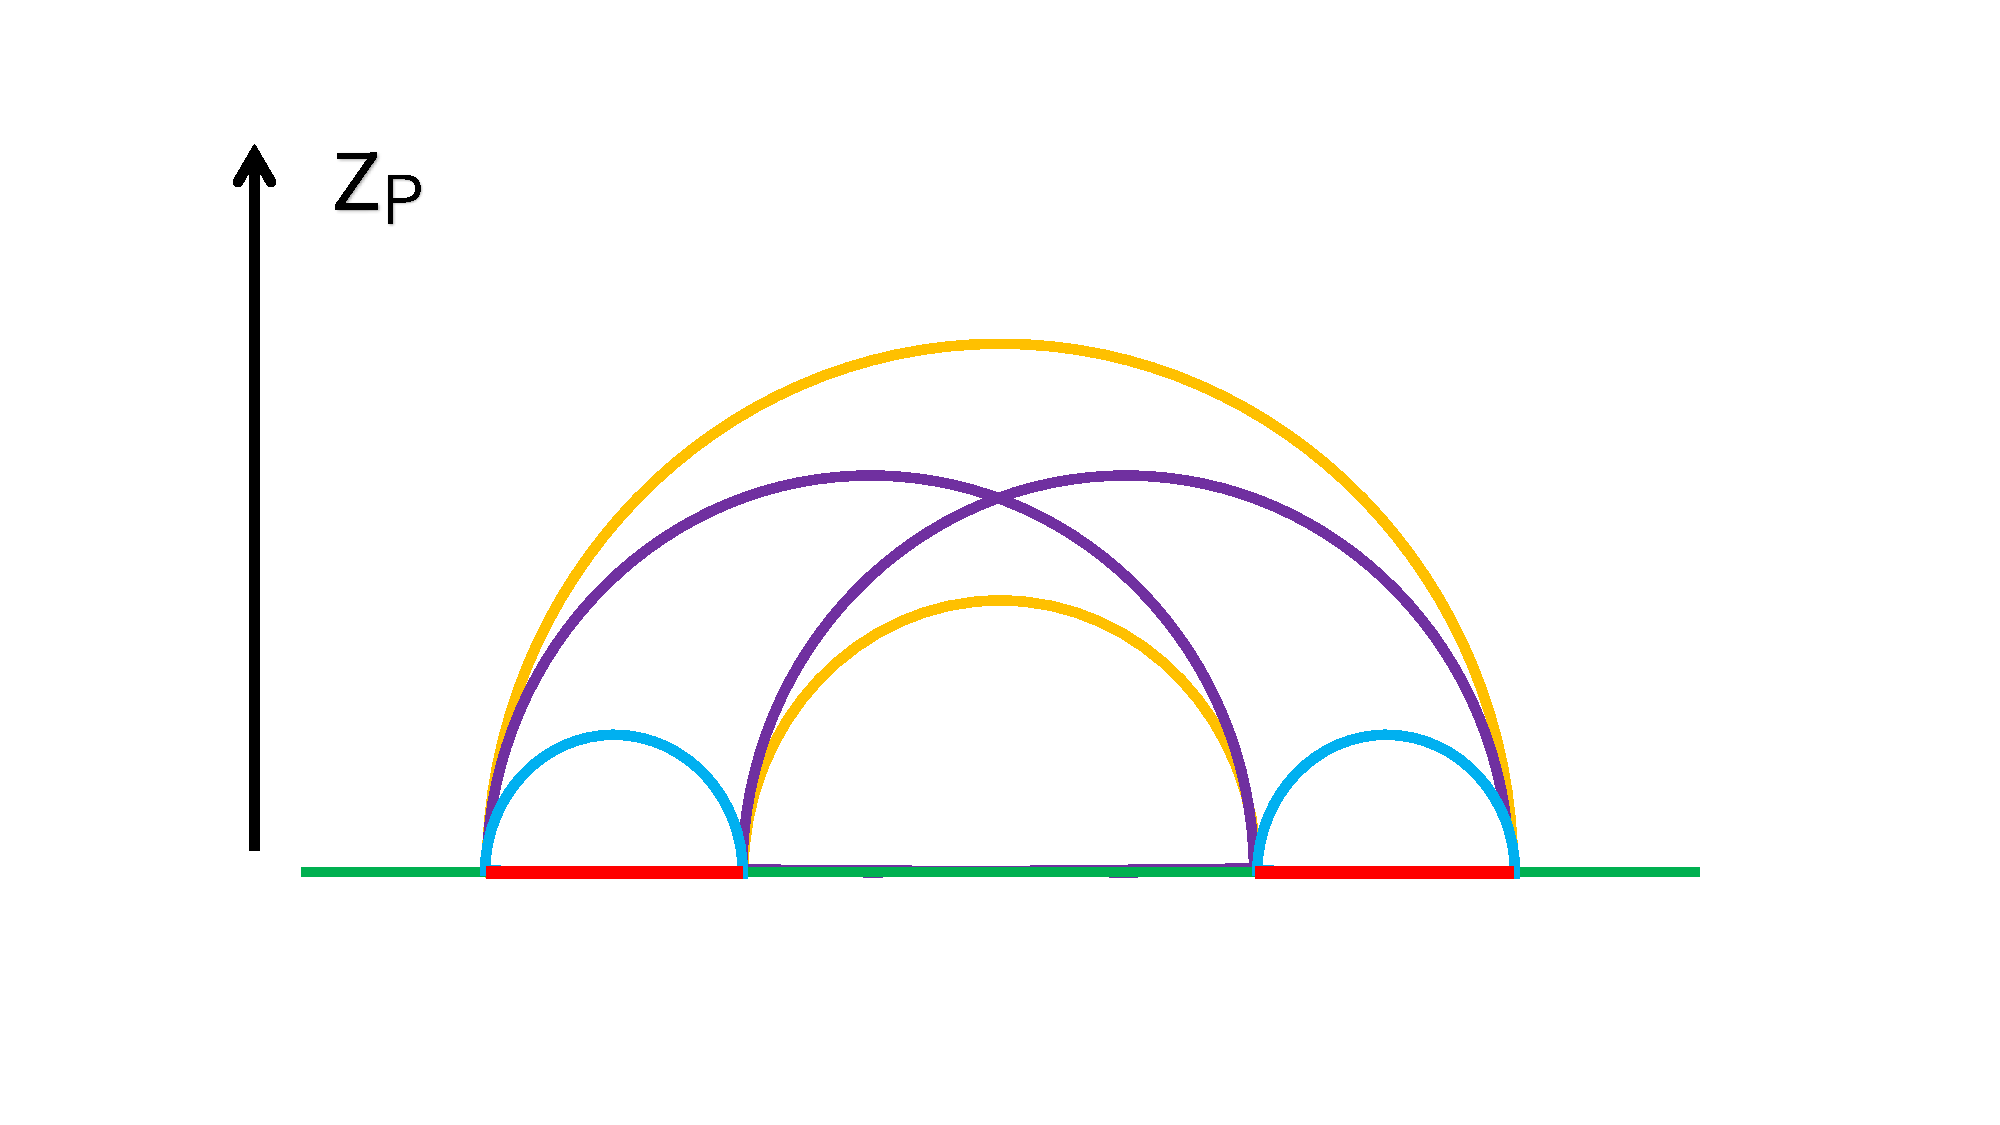
\includegraphics[width=0.7\linewidth]{disconnRTsurface.pdf}
	\label{fig:disconnRTsurface}
	\caption{Poincare座標の境界に定義された、2次元共形場理論の部分系$N=2$の部分系(赤い部分)と、その境界から伸ばした測地線の図。オレンジ・紫・水色の3通りの伸ばし方が考えられる。}
\end{figure}

よって右辺は
\begin{align}
RHS&=\frac{R_A}{2G}\log \frac{\min \left\{ |x_1-x_2|||x_3-x_4|, |x_1-x_3|||x_2-x_4|, |x_1-x_4|||x_2-x_3| \right\}}{\epsilon^2}\\
&=\frac{R_A}{2G}\log \frac{\min \left\{ |x_1-x_2|||x_3-x_4|, |x_1-x_4|||x_2-x_3| \right\}}{\epsilon^2}
\end{align}
となる。したがってAdS$_3$/CFT$_2$対応から、この場合も確かに笠-高柳公式が成立することが分かる。

$|x_1-x_2|||x_3-x_4|$の測地線と非連結区間Aで作られるループは2つの連結成分をもち、この測地線はしばしば\textbf{disconnected geodesic}と呼ばれる。また、$|x_1-x_4|||x_2-x_3|$の測地線と非連結区間Aで作られるループは1つの連結成分をもち、この測地線はしばしば\textbf{connected geodesic}と呼ばれる。

また、$|x_1-x_3|||x_2-x_4|$の寄与が現れないことは、エンタングルメントエントロピーの強劣加法性に対応している。実際、強劣加法性(\ref{ssa})から左辺のエンタングルメントエントロピーに対して
\begin{align}
S(\rho_{[x_1,x_2]})+S(\rho_{[x_3,x_4]})\le S(\rho_{[x_1,x_3]})+S(\rho_{[x_2,x_4]})
\end{align}
が成り立つので、$|x_1-x_3|||x_2-x_4|$の寄与が現れることは無い。このことは右辺では$\min$をとる操作によって実現されている。

\subsub{具体例5 : 円筒上のCFTの低温状態での、連結区間Aのエンタングルメントエントロピー}
半径$L$の円筒上の温度$\beta\gg L$の低温状態$\rho=e^{-\beta H}$について、連結区間$A=[x_1,x_2]$に対して笠-高柳公式の両辺を計算する。

一般にトーラス2点関数の計算は、平面上の2点関数のように中心電荷のみでは決まらないが、$\beta\gg 1$の極限を考えると、
\begin{align}
LHS\sim \frac{c}{3}\log \left(\frac{2L}{\epsilon}\sin\left(\frac{x_1-x_2}{2L}\right)\right)
\end{align}
となる。これは真空の場合の結果に整合している。

この共形場理論に対応する時空は温度$\beta_A\gg 1$のthermal AdSであり、右辺は
\begin{align}
RHS=\frac{\text{length}(\gamma)}{4G}=\frac{R_A}{2G}\log \left(\frac{2L}{\epsilon}\sin\left(\frac{x_1-x_2}{2L}\right)\right)
\end{align}
となる。したがってAdS$_3$/CFT$_2$対応から、この場合も確かに笠-高柳公式が成立することが分かる。

\subsub{具体例6 : 円筒上のCFTの高温状態での、小さな連結区間Aのエンタングルメントエントロピー}
半径$L$の円筒上の温度$\beta\ll L$の高温状態$\rho=e^{-\beta H}$について、小さな連結区間$A=[x_1,x_2],\ |x_1-x_2|\ll L$に対して笠-高柳公式の両辺を計算する。この場合も平面上の有限温度状態の場合と同じで、
\begin{align}
LHS&=S(\rho_A)=\frac{c}{3}\log\left(\frac{2\beta}{\epsilon}\sinh\left(\frac{x_1-x_2}{2\beta}\right)\right)\\
RHS&=\frac{\text{length}(\gamma)}{4G}=\frac{R_A}{2G}\log \left(\frac{2\beta R_A^{-1}}{\epsilon'}\sinh\left(\frac{x_1-x_2}{2\beta R_A^{-1}}\right)\right)
\end{align}
となり、AdS$_3$/CFT$_2$対応から、この場合も確かに笠-高柳公式が成立することが分かる。

\subsub{具体例7: 円筒上のCFTの高温状態での、全体系のエントロピー}
半径$L$の円筒上の温度$\beta\ll L$の高温状態$\rho=e^{-\beta H}$について、全体系に対して笠-高柳公式の両辺を計算する。左辺は単にカノニカル分布$\rho=e^{-\beta H}$のvon Neumannエントロピーであり、$\beta\gg L$より(\ref{cardyCE})から
\begin{align}
LHS\sim \frac{c}{3}\pi \beta^{-1}
\end{align}
となる。また右辺のホモロジー条件を満たす最小測地線は、BTZブラックホールのホライズンを1周するような曲線であり、(\ref{btzwindingcurvelength})より、
\begin{align}
RHS=\frac{2\pi R_A^2\beta_A^{-1}}{4G}=\frac{c_A}{3}\pi R_A\beta_A^{-1}
\end{align}
となる。AdS$_3$/CFT$_2$対応から、この場合も確かに笠-高柳公式が成立することが分かる。また、このことは笠-高柳公式がBekenstein-Hawking公式の一般化になっていることを表す。

\subsection{HRT公式}
笠-高柳公式は、Euclid時間の理論に対する公式である。笠-高柳公式のLorentz時間への拡張は、Hubeny,Rangamani,高柳\cite{Hubeny:2007xt}によって提案されている。この提案は次のようなものである。

$A$が定義されているCFTの時刻$t=t_\ast$のCauchy面を境界に持つような重力側のCauchy面$\Sigma$をとるごとに、上の境界条件とホモロジー条件を満たす長さ最小の曲線$\gamma_\Sigma \of \Sigma$が決まり、$\gamma_\Sigma$の長さのうち最大のものが、エンタングルメントエントロピーを与える。
\begin{oframed}
\begin{align}
S_A(t_\ast)=\max_{\del\Sigma=(t=t_\ast\text{面})} \min_{\substack{\gamma_\Sigma\of\Sigma\\ \del\gamma_\Sigma=\del A\\ \gamma_\Sigma\text{と}A\text{で作られるループは0にホモロガス}}} \frac{\text{Area}(\gamma_\Sigma)}{4G_N}
\end{align}
\end{oframed}

	\chapter{2次元共形場理論での分離クエンチ}\label{chap:singlquench}
\textbf{量子クエンチ(quantum quench)}とは、量子系の平衡状態$\rho$を用意して系のハミルトニアンのパラメータを瞬時に変化させることを指す。クエンチによってハミルトニアンが$H\to H'$と変わるため、一般には$\rho$は$H'$の平衡状態ではなくなり、$t\to \infty$で$H'$に対する平衡状態$\rho'$へ熱平衡化していく。このようなクエンチの問題設定は、孤立量子系の熱平衡化を調べる具体例の一つとして理論的に研究されてきた。近年の実験技術の発展により、冷却原子系を用いて孤立量子系を実現することが出来るようになって以降、様々な量子クエンチに対する系のダイナミクスの研究が理論・実験の双方からなされている。

2次元共形場理論の平衡状態を用意してクエンチしたときのエンタングルメントエントロピーの時間発展を調べる研究は、Calabrese,Cardy\cite{Calabrese2006}によって始まった。エンタングルメントエントロピーは部分系のエネルギー期待値と自由エネルギーの差なので、これを調べることでエンタングルメントによって生じた系の熱力学的なダイナミクスを調べることができる。特に、強結合な2次元共形場理論をクエンチしたときのエンタングルメントエントロピーの解析は、カオス性の強い系の平衡化を考える上でも興味深いが、一般には解析が難しい問題である。そこでAdS/CFT対応や笠-高柳公式を通して、AdS時空での測地線のダイナミクスに置き換えると、エンタングルメントエントロピーの時間発展を簡単に計算できるようになる。

この章では我々の研究\cite{Shimaji:2018czt}に基づき、直線上の共形場理論の真空を分離クエンチしたときのエンタングルメントエントロピーの時間発展を調べる。分離クエンチは実験的にも調べられており\cite{gring2012relaxation}、現実の系への応用を考える上でも興味深い。

\ref{sec:SPQsetup}節ではレプリカ法による計算のセットアップを説明し、\ref{sec:SPQdirac}節で零質量自由Dirac場での計算をする。そして\ref{sec:SPQholcft}節で重力双対を持つような2次元共形場理論でのエンタングルメントエントロピーの時間発展を計算し、AdS時空内の測地線を用いてその振る舞いを解釈する。

\section{問題設定}\label{sec:SPQsetup}
2次元共形場理論における分離クエンチとは、空間方向の1点での相互作用を時刻$t=0$で瞬時に``切る''ことを指す。切られた部分を境界として、分離によって因果的に独立な2つの領域$L,R$が生じる(図\ref{fig:sqlorentz})。
\begin{figure}[h]
	\centering
	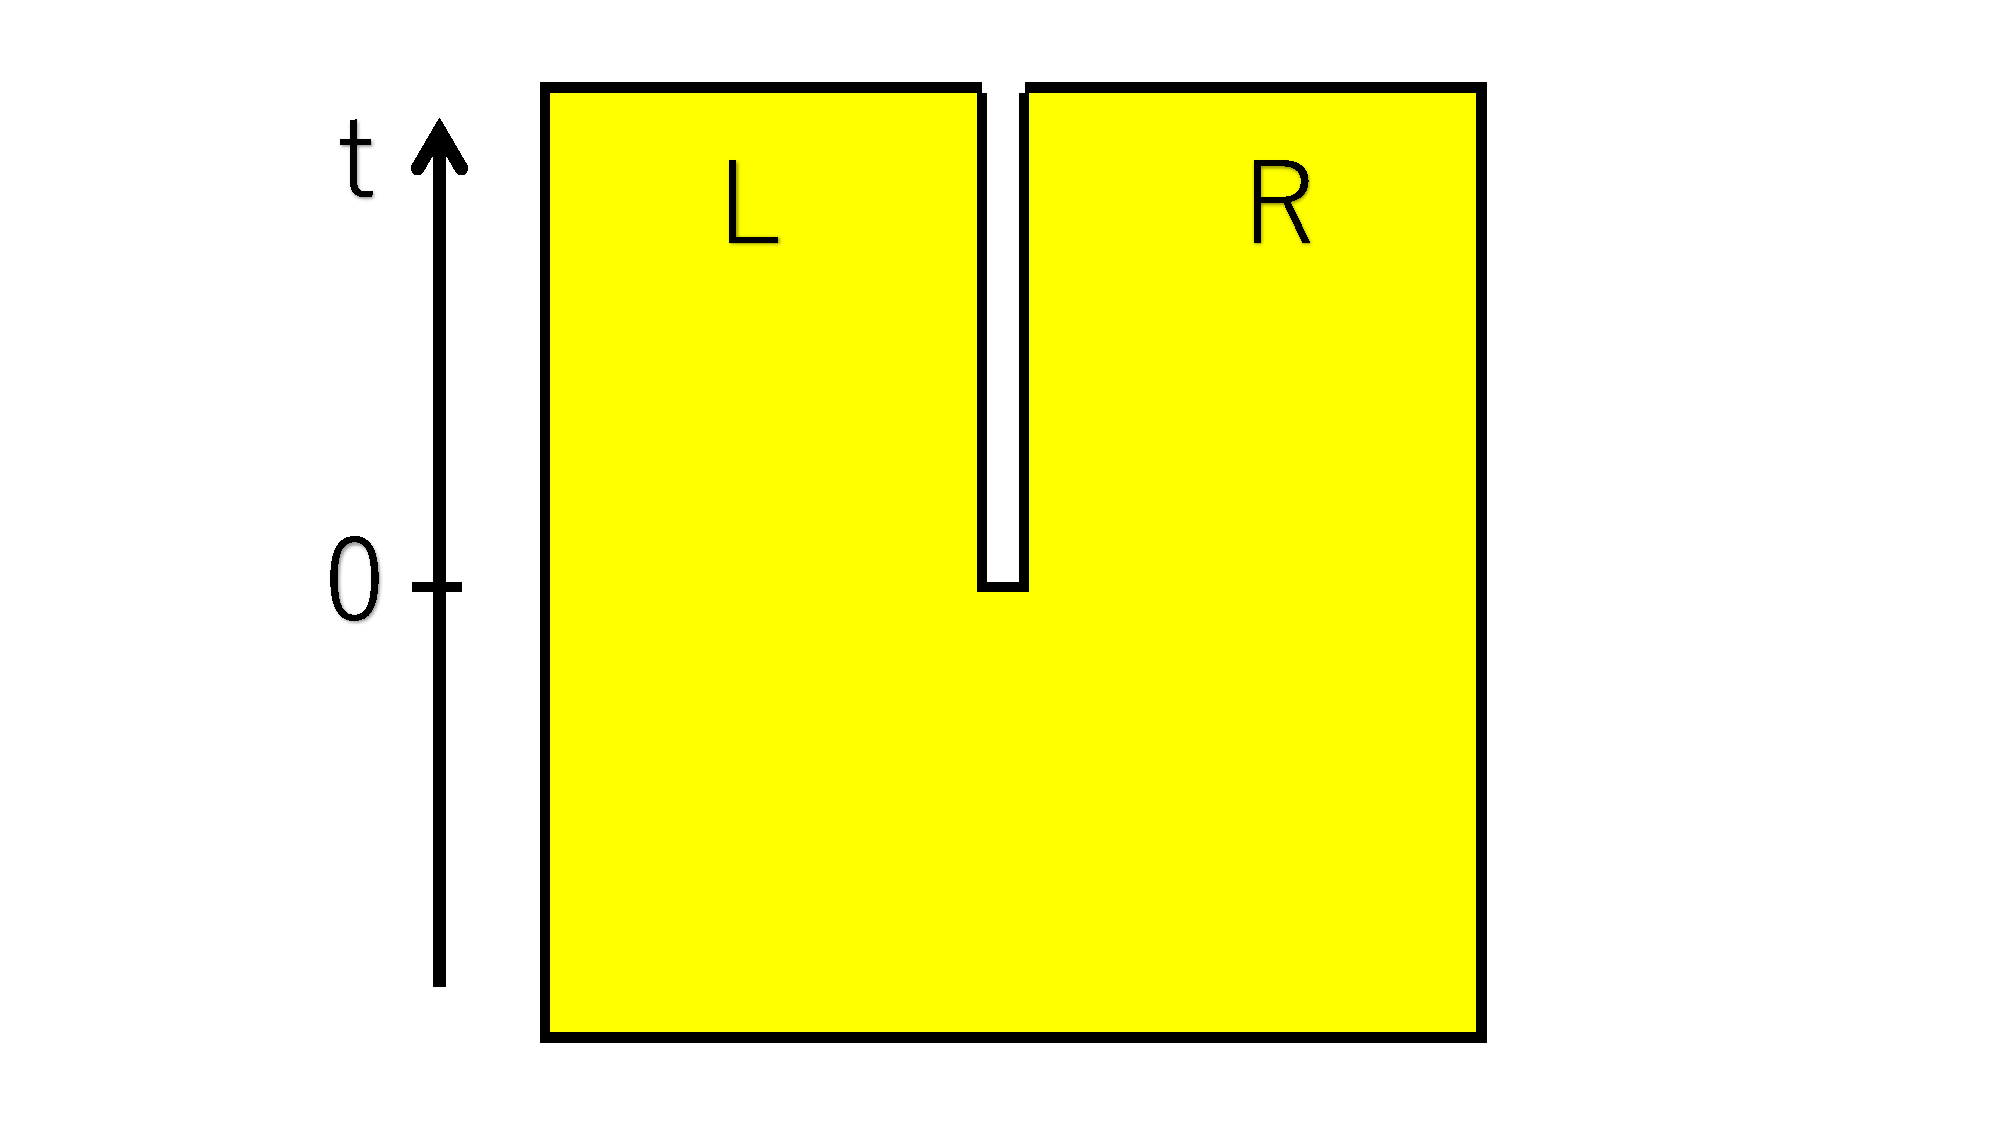
\includegraphics[width=0.7\linewidth]{SQlorentz.pdf}
	\label{fig:sqlorentz}
	\caption{分離クエンチされた系の図。分離によって因果的に独立な2つの領域$L,R$が生じる。}
\end{figure}

真空を分離クエンチした状態に対するエンタングルメントエントロピーをレプリカ法で計算するには、虚時間$\tau=-0,+0$面にクエンチされた状態$|\Psi\ra, \la\Psi|$を経路積分で用意して、注目系以外をトレースアウトしてorbifoldを作る。そして、実時間でのエンタングルメントエントロピーを得るには、レプリカ法で得た虚時間のエンタングルメントエントロピーの結果を$\tau\to 0+it$と解析接続する。

虚時間での経路積分は、区間$[-ia,ia]$に分離が入った平面$w=x+i\tau$座標(図\ref{fig:sqmapping})に対して行う。
\begin{figure}[h]
	\centering
	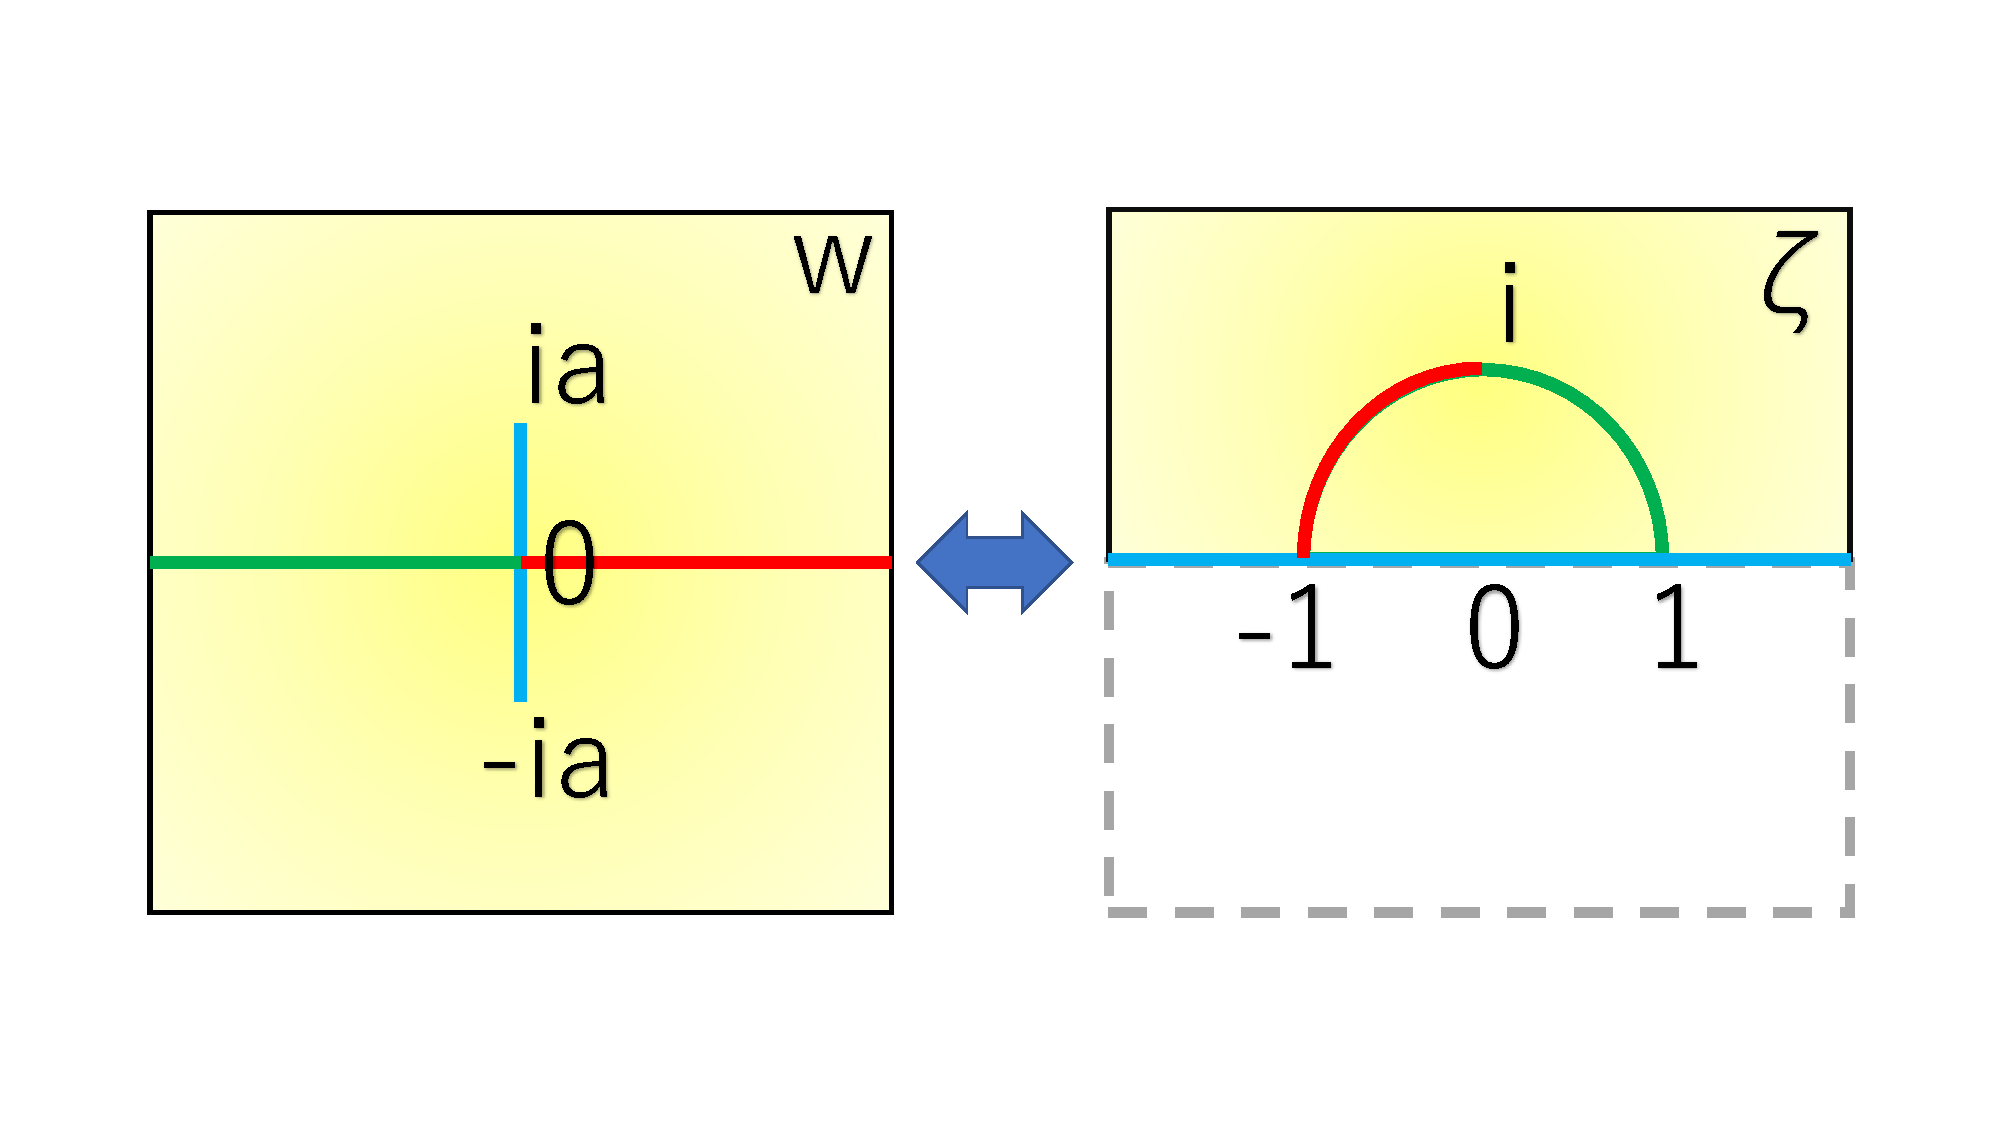
\includegraphics[width=0.7\linewidth]{SQmapping.pdf}
	\label{fig:sqmapping}
	\caption{左は分離クエンチされた真空についてのレプリカ法のセットアップの図。これを共形変換することで右の上半平面に移る。}
\end{figure}

$w$座標は共形変換
\begin{align}
\zeta=i\sqrt{\frac{w+ia}{w-ia}}\equiv f(w)
\end{align}
によって上半平面に移る。したがって虚時間でのエンタングルメントエントロピーの計算は、上半平面$\zeta$上に挿入されたツイスト演算子の相関関数を計算することに帰着される。

ここで、上の共形変換の根号を外すと、
\begin{align}
\zeta(x,\tau)&=\frac{-\ \text{sign}(x)\sqrt{A_{-}(x^2,\tau^2)}+i\sqrt{A_{+}(x^2,\tau^2)}}{\sqrt{2\left(x^2+(\tau-a)^2\right)}}\\
R(x^2,\tau^2)&=\sqrt{(x^2+\tau^2-a^2)^2+4a^2 x^2}\notag\\
&=\sqrt{(x^2+(\tau+a)^2)(x^2+(\tau-a)^2)}\\
A_\pm(x^2,\tau^2) &= R(x^2,\tau^2)\pm(x^2+\tau^2-a^2)
\end{align}
と書けて、さらに微分の絶対値は
\begin{align}
\left| \frac{d\zeta}{dw} \right|=\frac{a}{(R(x^2,\tau^2))^{1/2}\sqrt{x^2+(\tau-a)^2}}
\end{align}
となることに注意しておく。また、$R,A_\pm$は$\tau^2$のみに依存するので、$\tau\to it$の解析接続はそのまま実行できる。このとき、$a \downarrow 0$の極限で
\begin{align}
R(x^2,-t^2)&\sim |x^2-t^2|+\frac{x^2+t^2}{|x^2-t^2|}a^2  \\
A_{\pm}(x^2,-t^2)&\sim \left( |x^2-t^2|\pm (x^2-t^2) \right)+\left( \frac{x^2+t^2}{|x^2-t^2|}\mp 1 \right)a^2
\end{align}
と近似できることに注意しておく。これらの表式は後で使う。

\section{自由ディラック場}\label{sec:SPQdirac}
\subsub{解析計算}
共形境界条件としてNeumann境界条件またはDirichlet境界条件を考える。二重化のトリックを使うと下半平面に鏡像が現れ、Neumann/Dirichlet境界条件に応じてGreen関数は(\ref{scalarGreenUHP}),(\ref{scalarGreenCylinder})となるから、ツイスト演算子は境界条件を反映して
\begin{align}
&&&\text{Neumann}&\sigma_k(\zeta,\overline{\zeta})&=e^{i\frac{k}{n}(X_L(\zeta)-X_R(\overline{\zeta}))}\notag\\
&&&&&=V_{(k/n,-k/n)}(\zeta,\overline{\zeta})&&\left(k=-\frac{n-1}{2},-\frac{n-3}{2},\cdots \frac{n-1}{2}\right)\\
&&&\text{Dirichlet}&\sigma_k(\zeta,\overline{\zeta})&=e^{i\frac{k}{n}(X_L(\zeta)+X_R(\overline{\zeta}))}\notag\\
&&&&&=V_{(k/n,k/n)}(\zeta,\overline{\zeta})&&\left(k=-\frac{n-1}{2},-\frac{n-3}{2},\cdots \frac{n-1}{2}\right)
\end{align}
となる。

区間$[x_1,x_2]$に対するエンタングルメントエントロピーは上のツイスト演算子の2点関数を計算すればよく、NeumannとDirichletで同じ結果が得られる。
\begin{align}
S_A&=-\frac{1}{6}\log (F\epsilon^2)\\
F&=\left|\frac{d\zeta_1}{dw_1}\right|\left|\frac{d\zeta_2}{dw_2}\right|
\frac{(\zeta_1-\overline{\zeta}_2)(\overline{\zeta}_1-\zeta_2)}{|\zeta_1-\overline{\zeta}_1||\zeta_2-\overline{\zeta}_2|(\zeta_1-\zeta_2)(\overline{\zeta}_1-\overline{\zeta}_2)}
\end{align}

いま
\begin{align}
Q(x_1^2,x_2^2,\tau^2)&= \sqrt{(x_1^2+(\tau-a)^2)(x_2^2+(\tau+a)^2)}+(x_1\leftrightarrow x_2)\\
&=\sqrt{2}\sqrt{(x_1^2+\tau^2+a^2)(x_2^2+\tau^2+a^2)-4a^2\tau^2+R(x_1^2,\tau^2)R(x_2^2,\tau^2)}
\end{align}
と書くと、
\begin{align}
|\zeta_1-\zeta_2|^2&=\frac{ Q-\text{sign}(x_1x_2)\sqrt{A_{-1}A_{-2}}-\sqrt{A_{+1}A_{+2}} }{\sqrt{x_1^2+(\tau-a)^2}\sqrt{x_2^2+(\tau-a)^2}}\\
|\zeta_1-\overline{\zeta}_2|^2&=\frac{ Q-\text{sign}(x_1x_2)\sqrt{A_{-1}A_{-2}}+\sqrt{A_{+1}A_{+2}} }{\sqrt{x_1^2+(\tau-a)^2}\sqrt{x_2^2+(\tau-a)^2}}\\
|\zeta_1-\overline{\zeta}_1|&=\frac{\sqrt{2}\sqrt{A_{+1}}}{\sqrt{x_1^2+(\tau-a)^2}}
\end{align}
である。したがって$S_A$は$\tau^2$のみの関数として書けて、
\begin{align}
S_A=\frac{1}{6}\log \left( \frac{2R_1^{1/2}R_2^{1/2}A_{+1}^{1/2}A_{+2}^{1/2}(Q-\text{sign}(x_1x_2)\sqrt{A_{-1}A_{-2}}-\sqrt{A_{+1}A_{+2}})}{a^2\epsilon^2(Q-\text{sign}(x_1x_2)\sqrt{A_{-1}A_{-2}}+\sqrt{A_{+1}A_{+2}})} \right)
\end{align}
となり、解析接続$\tau\to it$はそのまま実行される。いま$|x_1|<|x_2|$として、$a\downarrow 0$の極限をとれば
\begin{align}
Q(x_1^2,x_2^2,-t^2)&\sim \sqrt{2}\sqrt{|(x_1^2-t^2)(x_2^2-t^2)|+(x_1^2-t^2)(x_2^2-t^2)+Q_2 a^2}\\
Q_2&=(x_1^2+t^2)\left(1+\frac{|x_2^2-t^2|}{|x_1^2-t^2|}\right)+(x_1\leftrightarrow x_2)
\end{align}
より、$a\downarrow 0$の極限での$S_A$の近似式は
\begin{align}
S_A(t)\sim \left\{ \begin{array}{ll}
\bigskip\dfrac{1}{3}\log\dfrac{|x_2-x_1|}{\epsilon}  &(0<t<|x_1|)\\
\bigskip\dfrac{1}{6}\log \dfrac{4|x_1|(x_2-x_1)(t-|x_1|)(x_2^2-t^2)}{(x_1+x_2)(t+|x_1|)a\epsilon^2} &(|x_1|<t<|x_2|)\\
\bigskip\dfrac{1}{6}\log \dfrac{4|x_1||x_2|(x_2-x_1)^2}{\epsilon^2(x_1+x_2)^2}  &(|x_2|<t,\ x_1x_2>0 )\\
\dfrac{1}{6}\log\dfrac{4|x_1||x_2|}{\epsilon^2} &(|x_2|<t,\ x_1x_2<0 )
\end{array}\right.
\end{align}
となる。とくに$t\to \infty$では
\begin{align}
S_A(t\to\infty) \sim \left\{ \begin{array}{ll}
\bigskip\dfrac{1}{6}\log \dfrac{4|x_1||x_2|(x_2-x_1)^2}{\epsilon^2(x_1+x_2)^2}  &(x_1x_2>0)\\
\dfrac{1}{6}\log\dfrac{4|x_1||x_2|}{\epsilon^2} &(x_1x_2<0)
\end{array}\right.
\end{align}
となる。

\subsub{数値計算}
上の計算を数値計算したものがグラフ\ref{fig:sd005}である。$a=0.05$で$S_A(t)$と真空のEE $S_\text{vac}=(1/3)\log(L/\epsilon)$の差$S_A(t)-S_\text{vac}$を計算しており、左図は部分系$[50,150]$,右図は$[-20,50]$にとった場合である。
\begin{figure}[h]
	\centering
	\begin{tabular}{c}
		\begin{minipage}{0.50\hsize}
			\centering
			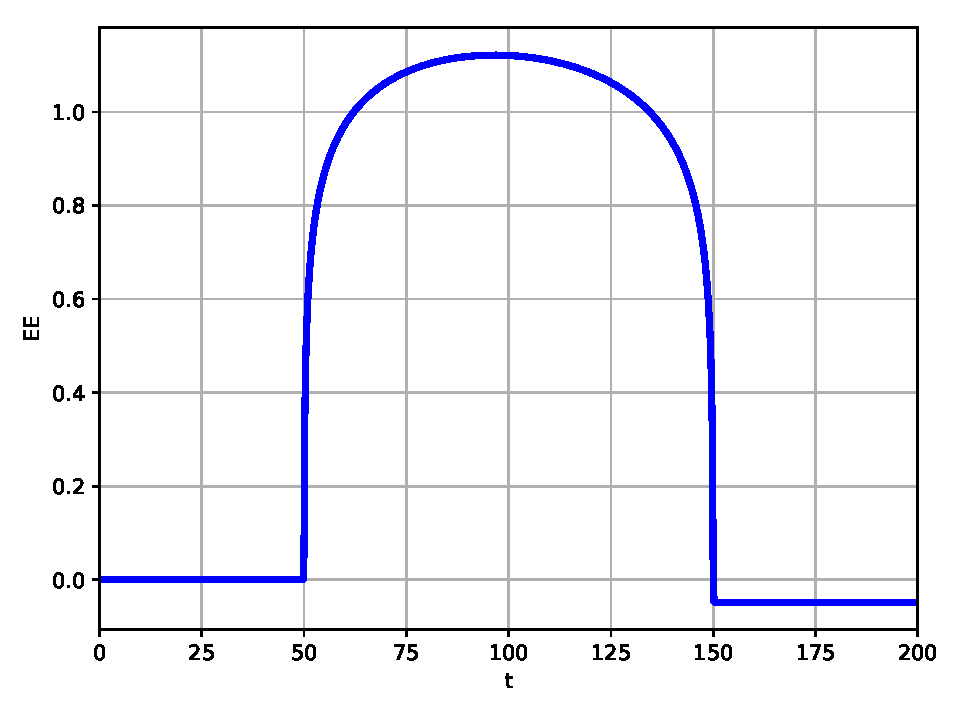
\includegraphics[width=\linewidth]{sd005_50_150.pdf}
		\end{minipage}
		\begin{minipage}{0.50\hsize}
			\centering
			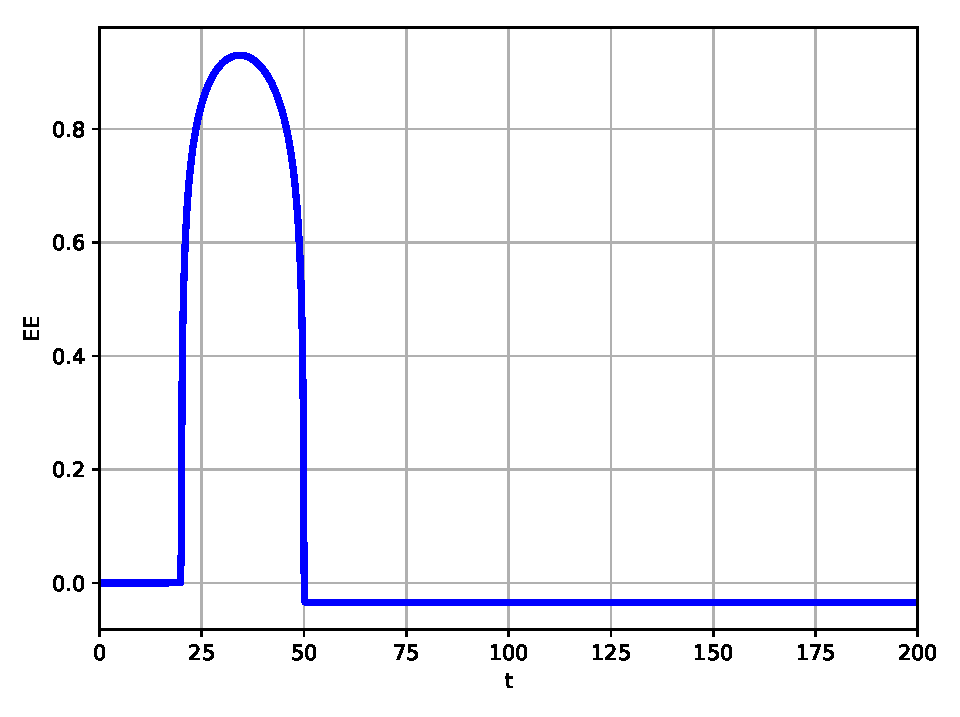
\includegraphics[width=\linewidth]{sd005_20_50.pdf}
		\end{minipage}
	\end{tabular}
	\caption{自由Dirac場の真空を分離クエンチしたときのEEのグラフ。横軸は時間$t$で、縦軸は真空の寄与を引いたEE $S_A(t)-S_\text{vac}$をプロットしている。}
	\label{fig:sd005}
\end{figure}
この結果は\cite{Calabrese:2007rg}で予想されたような、準粒子描像に当てはまっている。

\section{重力双対を持つ共形場理論}\label{sec:SPQholcft}
\subsection{AdS/BCFTの処方を用いたEEの解析}
\subsub{解析計算}
重力双対を持つ共形場理論でのエンタングルメントエントロピーは、笠・高柳公式やHRT公式を用いてAdS空間内の測地線の長さとして計算する。

いま$\zeta$座標は上半平面で定義されている。AdS/BCFTの処方から、$\zeta$座標に対応する境界付きAdS空間としてPoincare座標の上半分を考えることができる。このとき$\IM \zeta=0$面が境界$Q$になる(図\ref{fig:SQadsbcft})。
\begin{figure}[h]
	\centering
	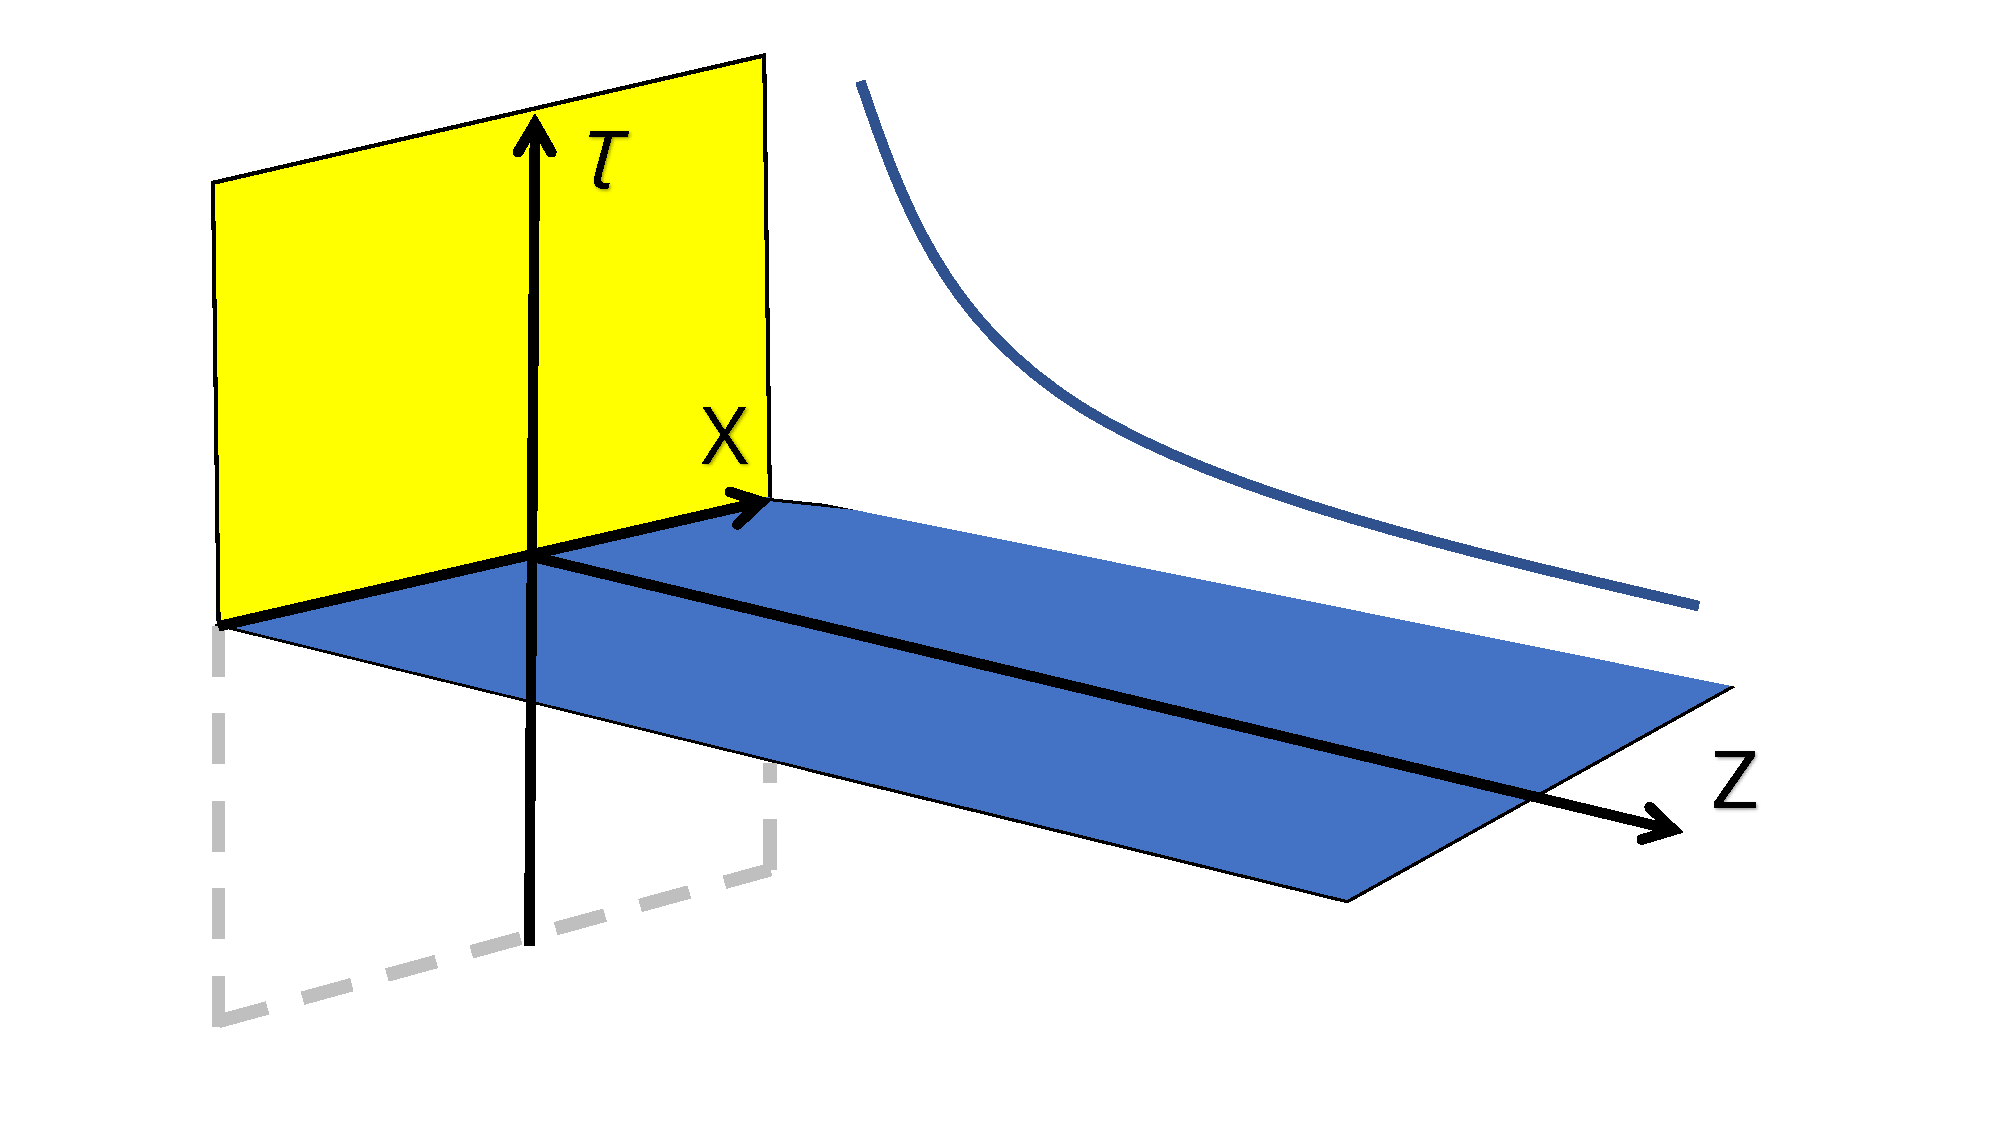
\includegraphics[width=0.7\linewidth]{UHPadsbcft.pdf}
	\label{fig:SQadsbcft}
	\caption{$\zeta$座標に対応する境界付きAdS空間の図。$\IM \zeta=0$面が、AdS/BCFTの処方でNeumann境界条件の課される境界$Q$になる。}
\end{figure}

$c\gg 1$近似を用いると、笠-高柳公式の測地線の候補としては、図(\ref{fig:sqrtsurfacecontraction})のように3つの取り方がある。
\begin{figure}[h]
	\centering
	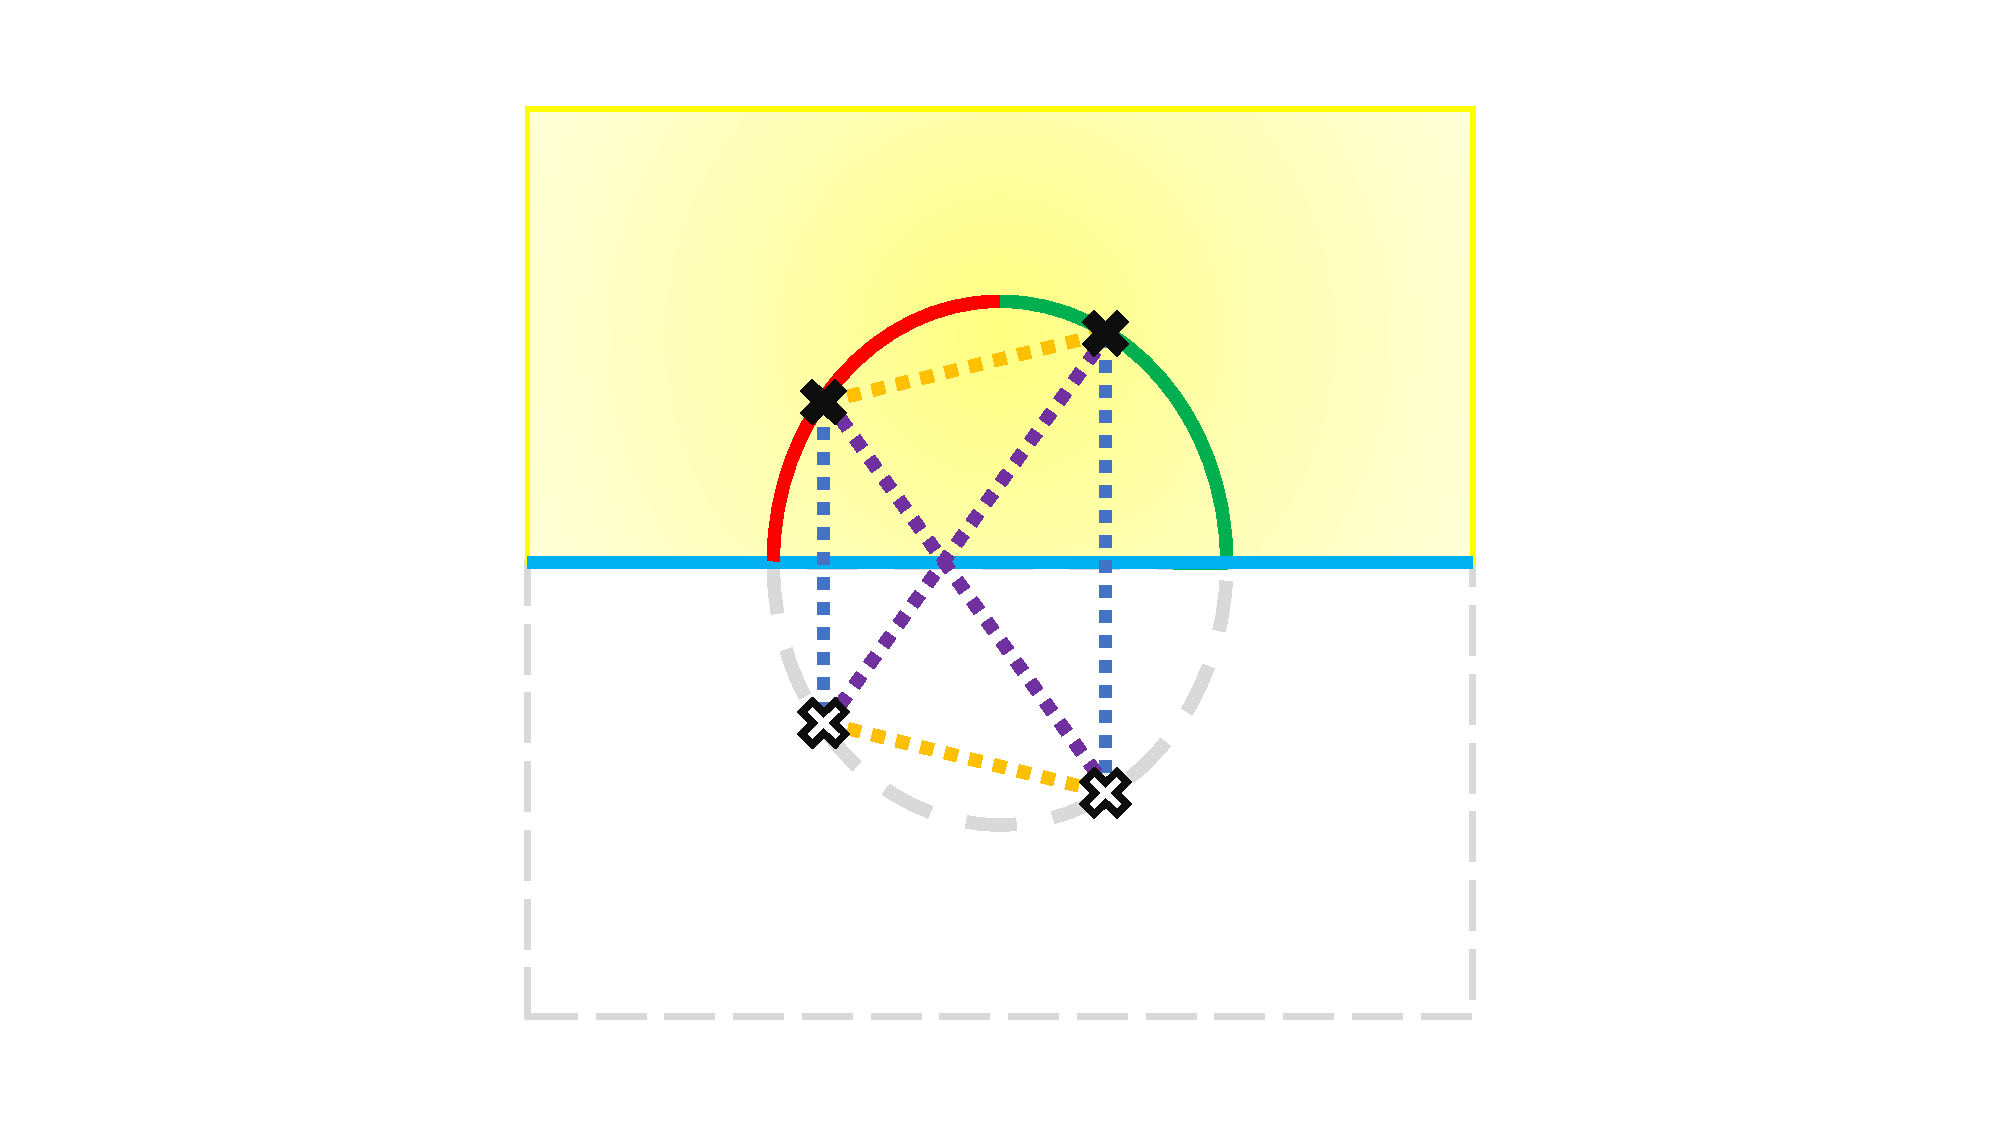
\includegraphics[width=0.7\linewidth]{SQRTsurfacecontraction.pdf}
	\label{fig:sqrtsurfacecontraction}
	\caption{測地線の取り方の図。AdS/BCFTの処方により、AdS空間に対しても``二重化のトリック''の類似を用いることができる。このとき下半平面に鏡像のツイスト演算子があると思って、笠-高柳公式の測地線の長さを計算すればよい。したがって測地線の候補として、オレンジ・紫・青の3つの取り方がある。}
\end{figure}

このときツイスト演算子の4つの挿入点は、必ず半径1の円に内接する四角形を描き、$\zeta_1,\overline{\zeta}_2$と$\zeta_2,\overline{\zeta}_1$を結ぶ測地線が最小となることは無い。したがって、このときも同様に測地線の候補として、$\zeta_1=f(w_1)$と$\zeta_2=f(w_2)$を結ぶ曲線と、$\zeta_1,\zeta_2$がそれぞれの鏡像点$\overline{\zeta}_1,\overline{\zeta}_2$と結ぶ曲線の2種類の取り方があり、それぞれをconnected geodesic, disconnected geodesicと呼ぶことにする。それぞれの測地線に対するエントロピーは
\begin{align}
S^{con}_A&=\frac{c}{6}\log\left(\frac{|f(w_1)-f(w_2)|^2}{\delta_1\delta_2}\right)\\
S^{dis}_A&=\frac{c}{6}\log\left(\frac{4(\IM f(w_1))(\IM f(w_2))}{\delta_1\delta_2}\right)
\end{align}
である。ただし$\delta_i\ (i=1,2)$はPoincare座標での紫外カットオフであり、元の$w$座標に対応する境界付き漸近的AdS空間での紫外カットオフ$\epsilon$との関係は、(\ref{robertsmapz})で$z\sim 0$の極限を考えることで、
\begin{align}
\epsilon |f'(w_i)|=\delta_i\label{cutofftransf}
\end{align}
と関係していることが分かる。

ホログラフィックな共形場理論でのエンタングルメントエントロピーはこれらのうちの小さいほうで求められる。
\begin{align}
S_A(t)=\min \{S^{con}_A(t),S^{dis}_A(t) \}
\end{align}

Dirac場での計算と同様に、$\tau\to it$と解析接続したときの$S^{con}_A(t),S^{dis}_A(t)$の$a\to 0$での近似式を求めると、次のようになる。

\subsub{connected geodesic}
$0<x_1<x_2$のとき
\begin{align}
S_{A}^{con}(t)\sim \frac{c}{6}\log\left\{
\begin{array}{ll}
\bigskip
\dfrac{(x_2-x_1)^2}{\epsilon^2}& (0<t<x_1)\\
\bigskip
\dfrac{2(x_2-x_1)(t-x_1)(x_2-t)}{a\epsilon^2}& (x_1<t<x_2)\\
\bigskip
\dfrac{(x_2-x_1)^2}{\epsilon^2}& (x_2<t)
\end{array}
\right.
\end{align}
$x_1<0<x_2,\ |x_1|<|x_2|$のとき
\begin{align}
S_{A}^{con}(t) \sim \frac{c}{6}\log\left\{
\begin{array}{ll}
\bigskip
\dfrac{(x_2-x_1)^2}{\epsilon^2}& (0<t<-x_1)\\
\bigskip
\dfrac{2(x_2-x_1)(t+x_1)(x_2+t)}{a\epsilon^2}& (-x_1<t<x_2)\\
\bigskip
\dfrac{4(t^2-x_1^2)(t^2-x_2^2)}{a^2\epsilon^2}& (x_2<t)\\
\end{array}
\right.
\end{align}
\subsub{disconnected geodesic}
$|x_1|<|x_2|$のとき
\begin{equation}
S_{A}^{dis} \sim \frac{c}{6}\log\left\{
\begin{array}{ll}
\bigskip
\dfrac{4(x_1^2-t^2)(x_2^2-t^2)}{a^2\epsilon^2}& (0<t<|x_1|)\\
\bigskip
\dfrac{4|x_1|(x_2^2-t^2)}{a\epsilon^2}& (|x_1|<t<|x_2|) \\
\bigskip
\dfrac{4|x_1||x_2|}{\epsilon^2}& (|x_2|<t)
\end{array}
\right.
\end{equation}

したがって$t\to\infty$での$S_A$は
\begin{align}
S_A(t\to\infty)\sim \left\{ \begin{array}{ll}
\bigskip
\min\left\{ \dfrac{c}{3}\log\dfrac{|x_2-x_1|}{\epsilon},\  \dfrac{c}{6}\log\dfrac{4|x_1||x_2|}{\epsilon^2} \right\} & (x_1x_2>0) \\
\bigskip
\dfrac{c}{6}\log\dfrac{4|x_1||x_2|}{\epsilon^2} & (x_1x_2<0) 
\end{array}\right.
\end{align}
となる。

\subsub{数値計算}
上の計算を数値計算したものがグラフ\ref{fig:sh005}である。$a=0.05$で$S_A(t)$と真空のEE$S_\text{vac}=(c/3)\log(L/\epsilon)$の差を計算しており、左図は部分系$[50,150]$,右図は$[-20,50]$にとった場合である。青線がconnected geodesicに対応するグラフで、赤線がdisconnecetd geodesicに対応するグラフであり、$S_A(t)$は2つの最小値である。
\begin{figure}[h]
	\centering
	\begin{tabular}{c}
		\begin{minipage}{0.50\hsize}
			\centering
			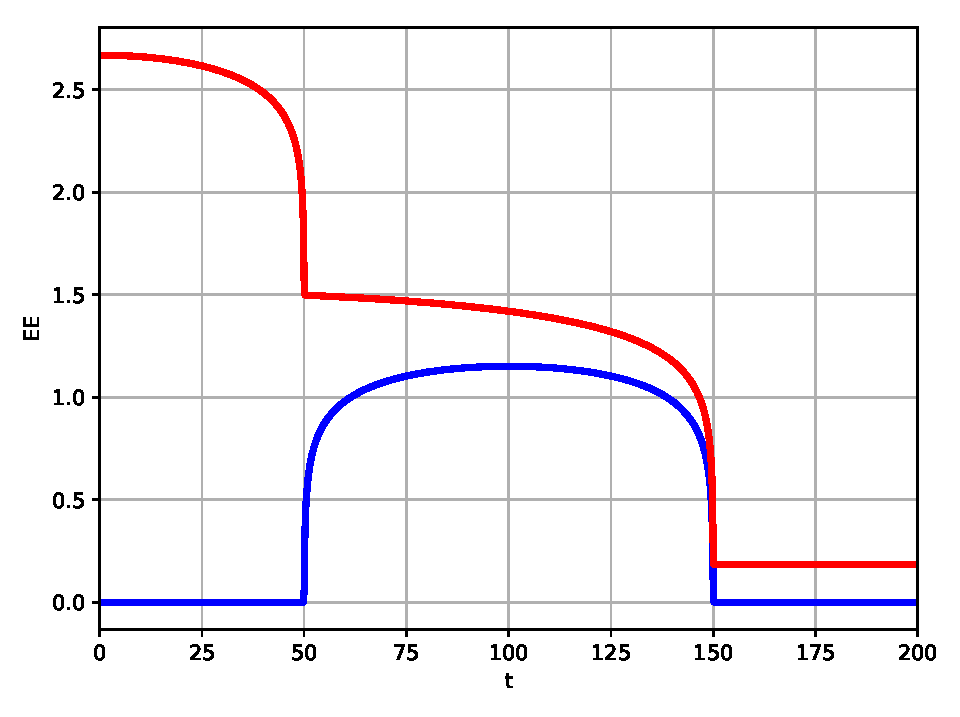
\includegraphics[width=\linewidth]{sh005_50_150.pdf}
		\end{minipage}
		\begin{minipage}{0.50\hsize}
			\centering
			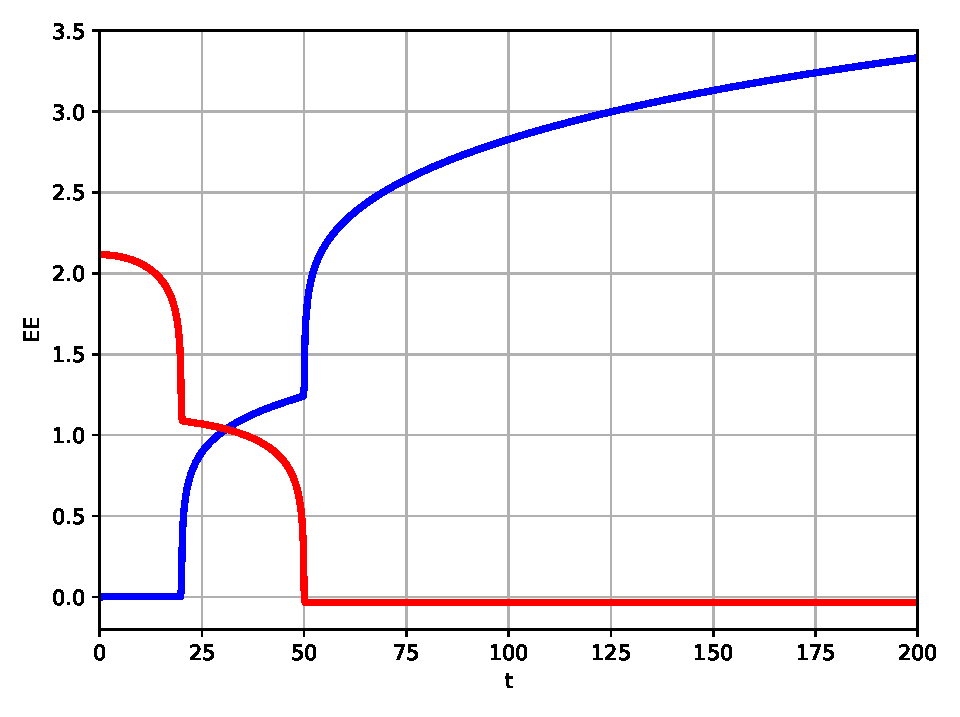
\includegraphics[width=\linewidth]{sh005_20_50.pdf}
		\end{minipage}
	\end{tabular}
	\caption{重力双対を持つ共形場理論の真空を分離クエンチしたときのEEのグラフ。横軸は時間$t$で、縦軸は真空の寄与を引いたEE $S_A(t)-S_\text{vac}$をプロットしている。青線がconnected geodesicに対応するグラフで、赤線がdisconnecetd geodesicに対応するグラフである。}
	\label{fig:sh005}
\end{figure}
この結果も準粒子描像に当てはまっている。

\subsection{AdS側での解釈}
ホログラフィックな共形場理論でのエンタングルメントエントロピー$S_A$をAdS空間の測地線の長さとして求めたが、ここでは$S_A$の振る舞いをAdS側の言葉で解釈してみる。

AdS/BCFTの処方により、上半平面$\zeta$の双対となるAdS時空をPoincare座標
\begin{align}
ds^2 = R_A^2 \frac{d\eta^2+d\zeta d\overline{\zeta}}{\eta^2},\ \IM \zeta>0
\end{align}
にとる。このとき(\ref{robertsmap1})(\ref{robertsmap2})(\ref{robertsmapz})の変換をすると、$w=x+i\tau$座標のホログラフィック共形場理論に対応する境界付きAdS空間の計量は、Feffermann-Graham計量の形で与えられ、
\begin{align}
ds^2&=R_A^2 \left( \frac{dz^2}{z^2}+L(w)dw^2+\overline{L}(\overline{w})d\overline{w}^2+\left( \frac{1}{z^2}+ z^2L(w)\overline{L}(\overline{w})\right)dwd\overline{w}  \right)\\
L(w)&=\frac{3(f'')^2-2f'f'''}{4f'^2}=\frac{3a^2}{4(w^2+a^2)^2}
\end{align}
である。

また、$(\zeta,\overline{\zeta},\eta)$と$(w,\overline{w},z)$は
\begin{align}
\zeta&=i\sqrt{\frac{w+ia}{w-ia}}\left( 1-ia\frac{2z^2(\overline{w}-ia)}{4|w^2+a^2|^2+z^2|2w+ia|^2} \right)\\
\eta&=a\frac{4z|w+ia|^{3/2}|w-ia|^{1/2}}{4|w^2+a^2|^2+z^2|2w+ia|^2}
\end{align}
で関係しており、上半分のPoincare座標では$\IM \zeta=0$にあったboundary surfaceは、この変換によって$Q=\{(x,\tau,z)\mid x=0, \tau\in [-a,a], z>0 \}$面に移ることが分かる。

このとき、計量$ds^2$の体積要素は
\begin{align}
\sqrt{\det(ds^2)}=\frac{R_A}{z^3}\sqrt{ (z^4L^2-1)(z^4\overline{L}^2-1)+z^4(L-\overline{L})^2}
\end{align}
である。

「$x\sim a$かつ$\tau=0$」あるいは「$x=0$かつ$\tau\sim a$」では$L\sim \frac{3}{16 a^2}$となるから、
\begin{align}
\sqrt{\det(ds^2)}\sim \frac{R_A}{z^3}\left|1-\left(\frac{\sqrt{3}z}{4a}\right)^4\right|
\end{align}
である。Poincare座標の体積要素は$R_A/z^3$であるから、虚時間のセットアップにおいて計量は「$x\sim a$かつ$\tau=0$」あるいは「$x=0$かつ$\tau\sim a$」で大きく曲がっていることが分かる。つまり$ds^2$はその境界$Q$付近で大きく曲がっており、境界$Q$はAdS$_3$時空のPoincare座標に存在する``非常に重い物体''として解釈できる。

したがって、Lorentz時間のセットアップを考えた時には、HRT公式から測地線は計量の$\det$の大きくなる境界近くに張り付くようになり、下図のようになる。
\begin{figure}[H]
	\centering
	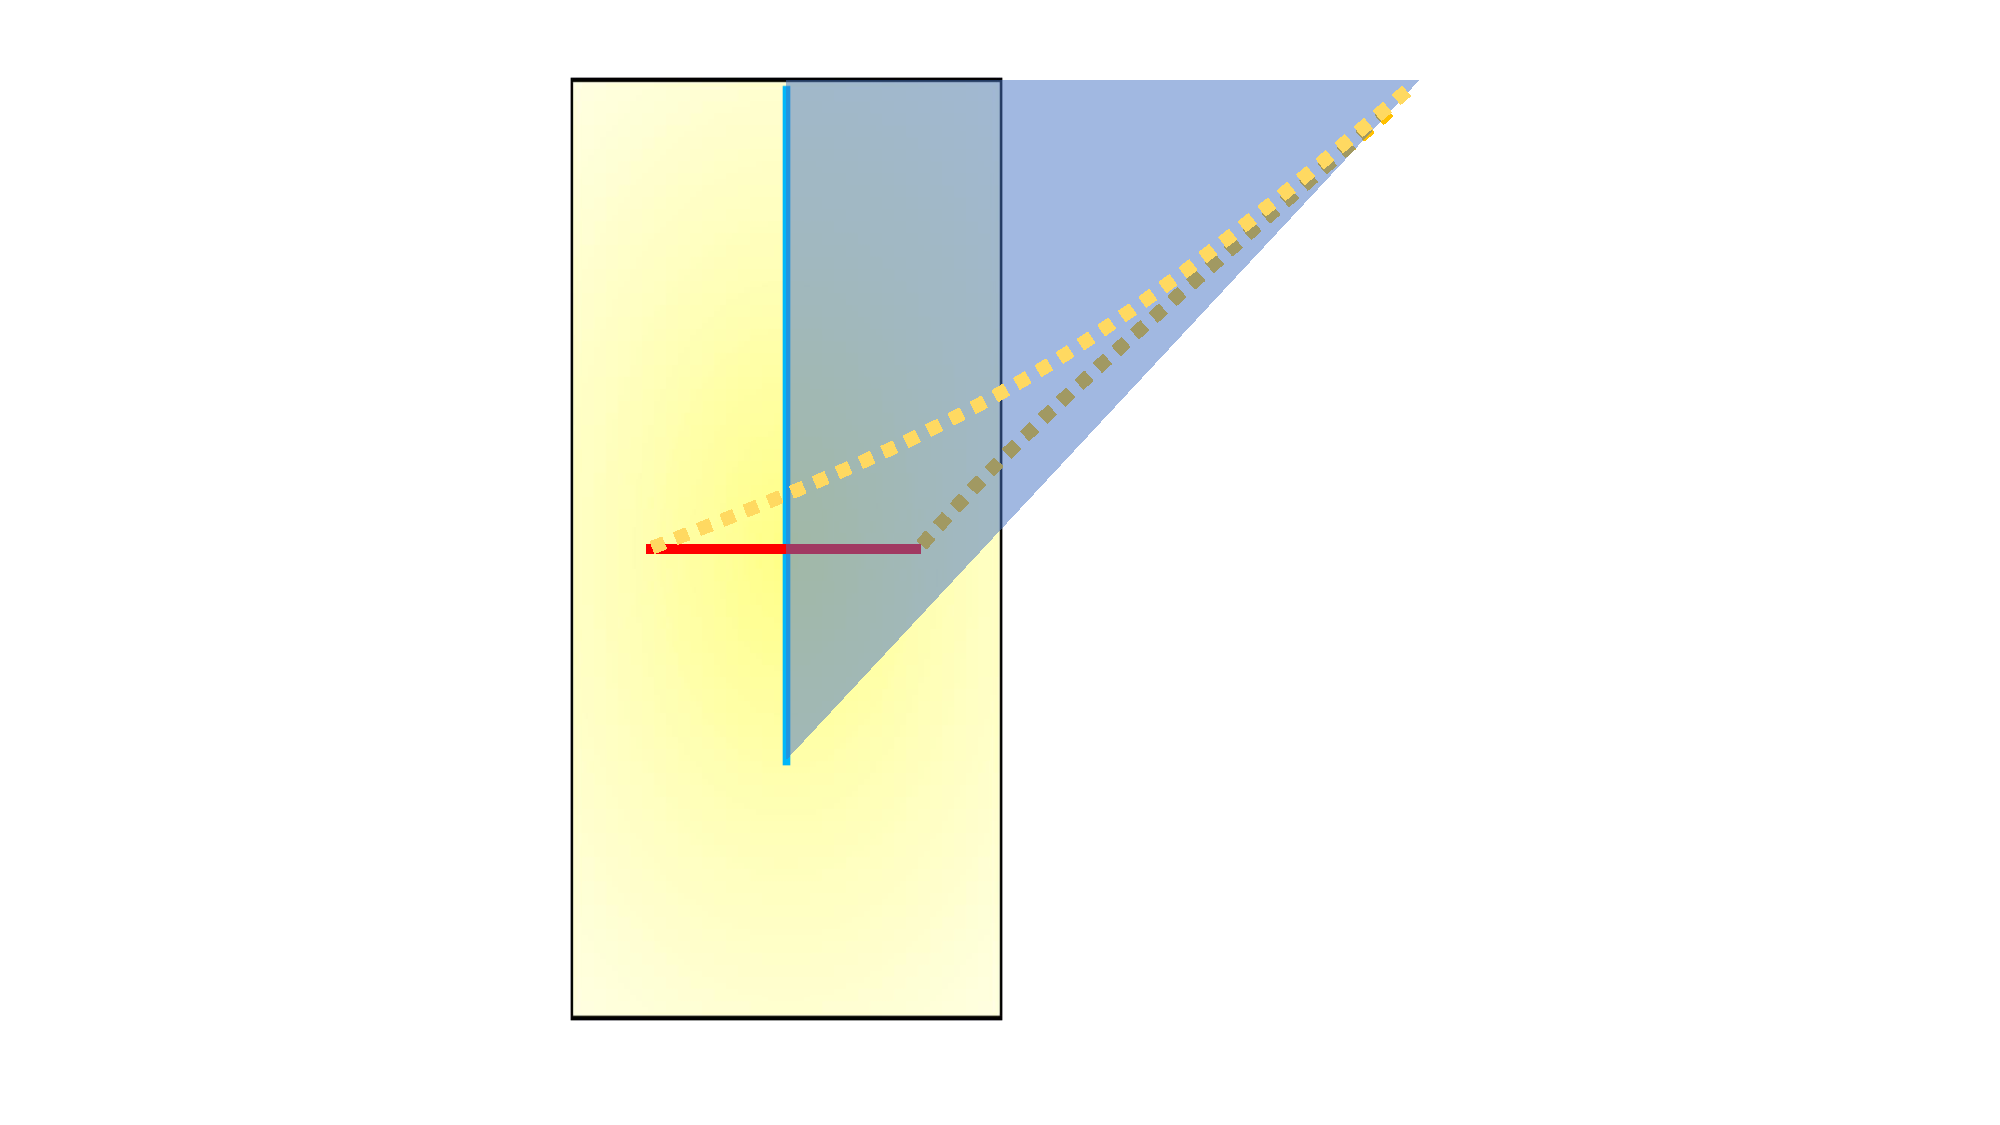
\includegraphics[width=0.7\linewidth]{SQgeod.pdf}
\end{figure}

したがって境界をまたぐ部分系で$t\to \infty$でconnected geodesicの長さが$\log$発散したのはこの境界によって障害が生まれたためであると考えられる。

	\chapter{2次元共形場理論での2重分離クエンチ}\label{chap:doublequench}
この章では我々の研究\cite{Caputa:2019avh}に基づき、直線上の共形場理論の真空を2重分離クエンチしたときのエンタングルメントエントロピーの時間発展を調べる。\ref{sec:DSQsetup}節ではレプリカ法による計算のセットアップを説明し、\ref{sec:DSQdirac}節で零質量自由Dirac場での計算をする。\ref{sec:DSQholcft}節で重力双対を持つような2次元共形場理論でのエンタングルメントエントロピーの時間発展を計算する。そして最後に\ref{sec:DSQSPQ}で1重分離クエンチと2重分離クエンチの違いについて論じる。前章で論じた(1重)分離クエンチの重力側での対応物は、AdS時空に非常に``重い"障害を与えたが、2重分離クエンチの対応物となる障害は互いに重力相互作用によって近づくと予想できる。この予想を、測地線の長さを測る笠-高柳公式によって確認した。

\section{問題設定}\label{sec:DSQsetup}
2次元共形場理論における2重分離クエンチとは、空間方向の異なる2点での相互作用を時刻$t=0$で瞬時に同時に``切る''ことを指す。切られた部分を境界として、分離によって因果的に独立な3つの領域$L,C,R$が生じる(図\ref{fig:dqlorentz})。
\begin{figure}[h]
	\centering
	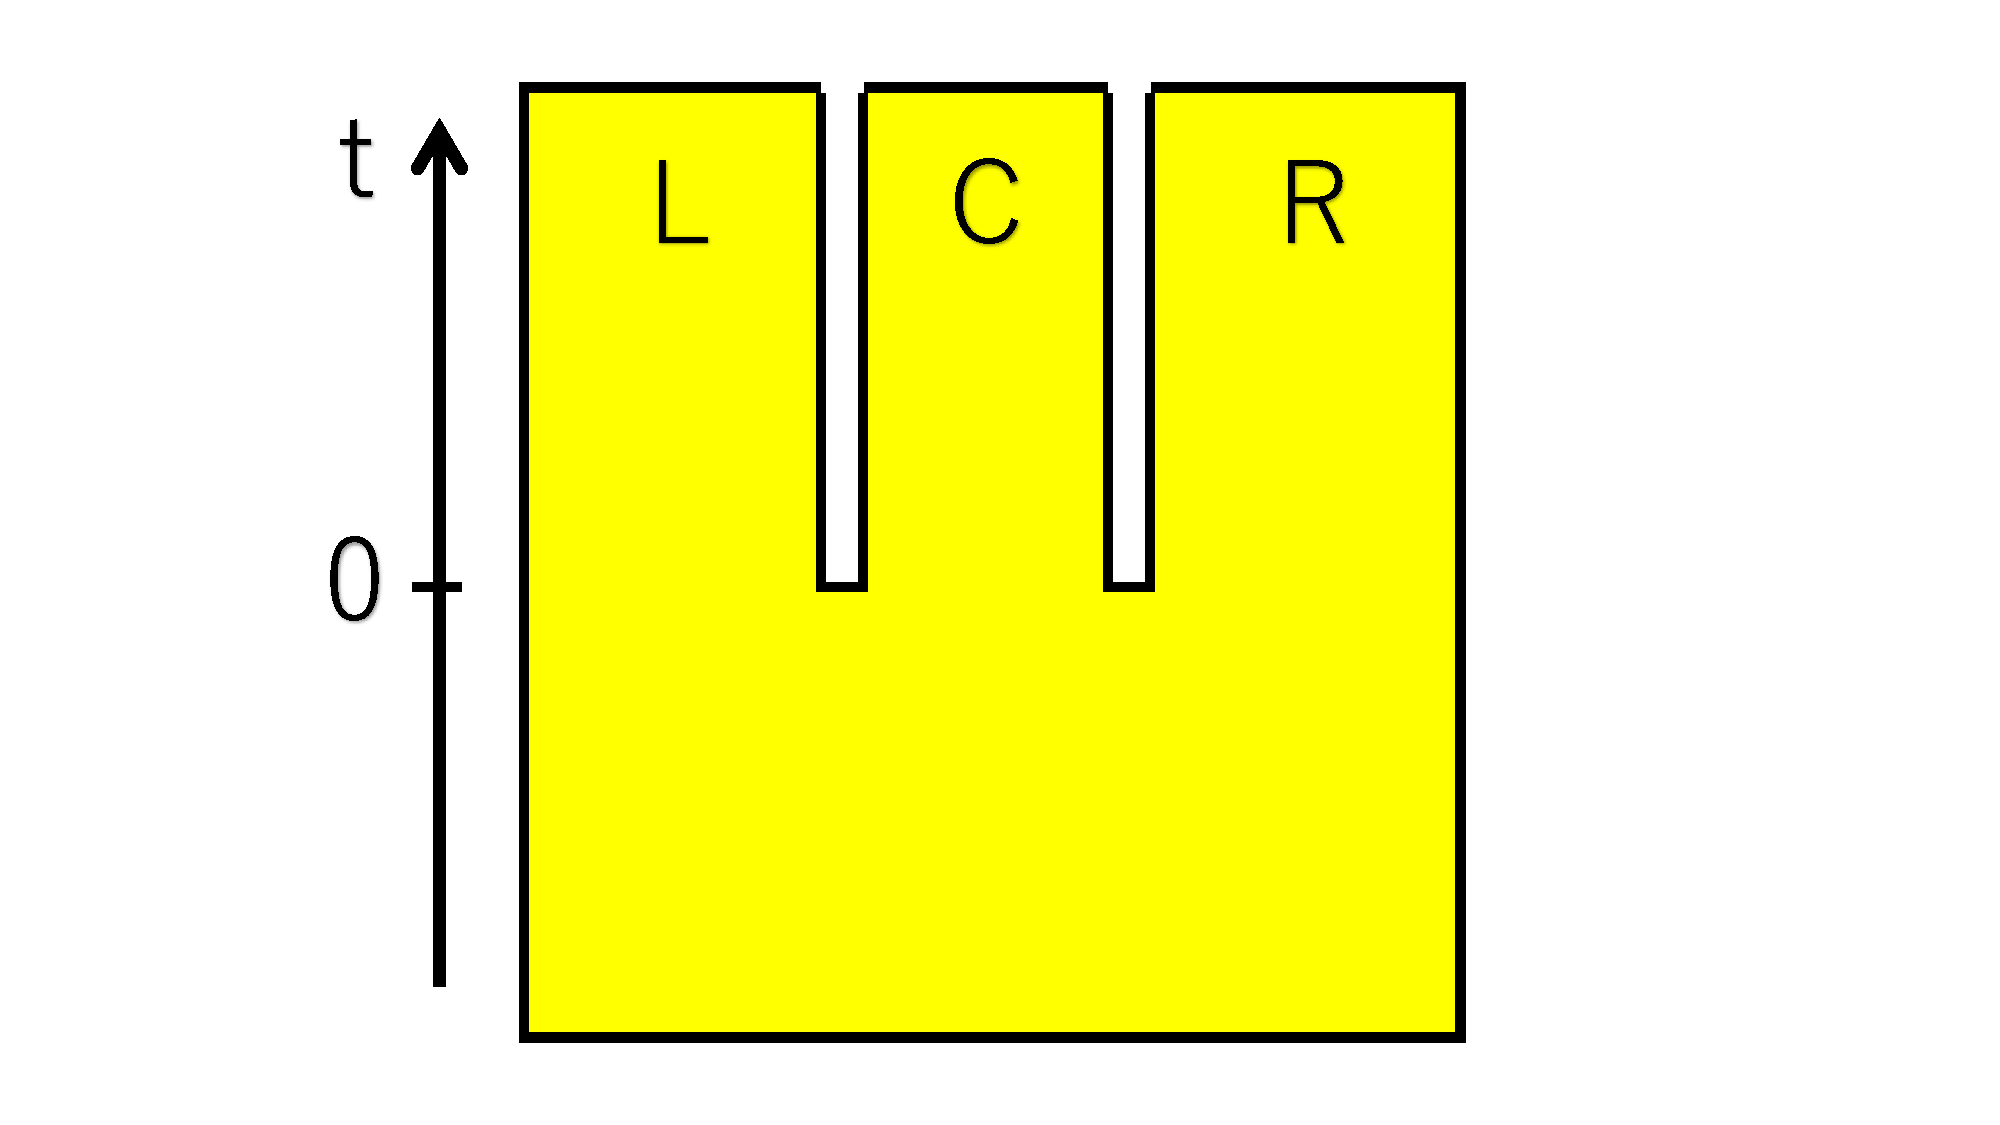
\includegraphics[width=0.7\linewidth]{DQlorentz.pdf}
	\label{fig:dqlorentz}
	\caption{2重分離クエンチされた系の図。分離によって因果的に独立な3つの領域$L,C,R$が生じる。}
\end{figure}

真空を分離クエンチした状態に対するエンタングルメントエントロピーをレプリカ法で計算するには、虚時間$\tau=-0,+0$面にクエンチされた状態$|\Psi\ra, \la\Psi|$を経路積分で用意して、注目系以外をトレースアウトしてorbifoldを作る。そして、実時間でのエンタングルメントエントロピーを得るには、レプリカ法で得た虚時間のエンタングルメントエントロピーの結果を$\tau\to 0+it$と解析接続する。

虚時間でのセットアップは$[\pm b-ia,\pm b+ia]$を2つの分離の境界とし図\ref{fig:dqmapping}で表される。これは
\begin{align}
w(\nu)&=x+i\tau=b\left( 1+ K_{\beta^{-1}}(\nu)+K_{\beta^{-1}}\left(\nu+\frac{i\beta^{-1}}{2}\right) \right)\\
K_{\beta^{-1}}(\nu)&=\frac{1}{\pi i}\left.\frac{\del}{\del \nu'}\log\theta_1(\nu',i\beta^{-1})\right|_{\nu'=\nu}
\end{align}
とすることで、$\IM \nu=\pm \beta^{-1}/4$に境界をもち、$\nu\sim \nu+1$と同一視の入った円筒に移る\cite{sakajo2012force}\cite{Numasawa_2016}。
\begin{figure}[h]
	\centering
	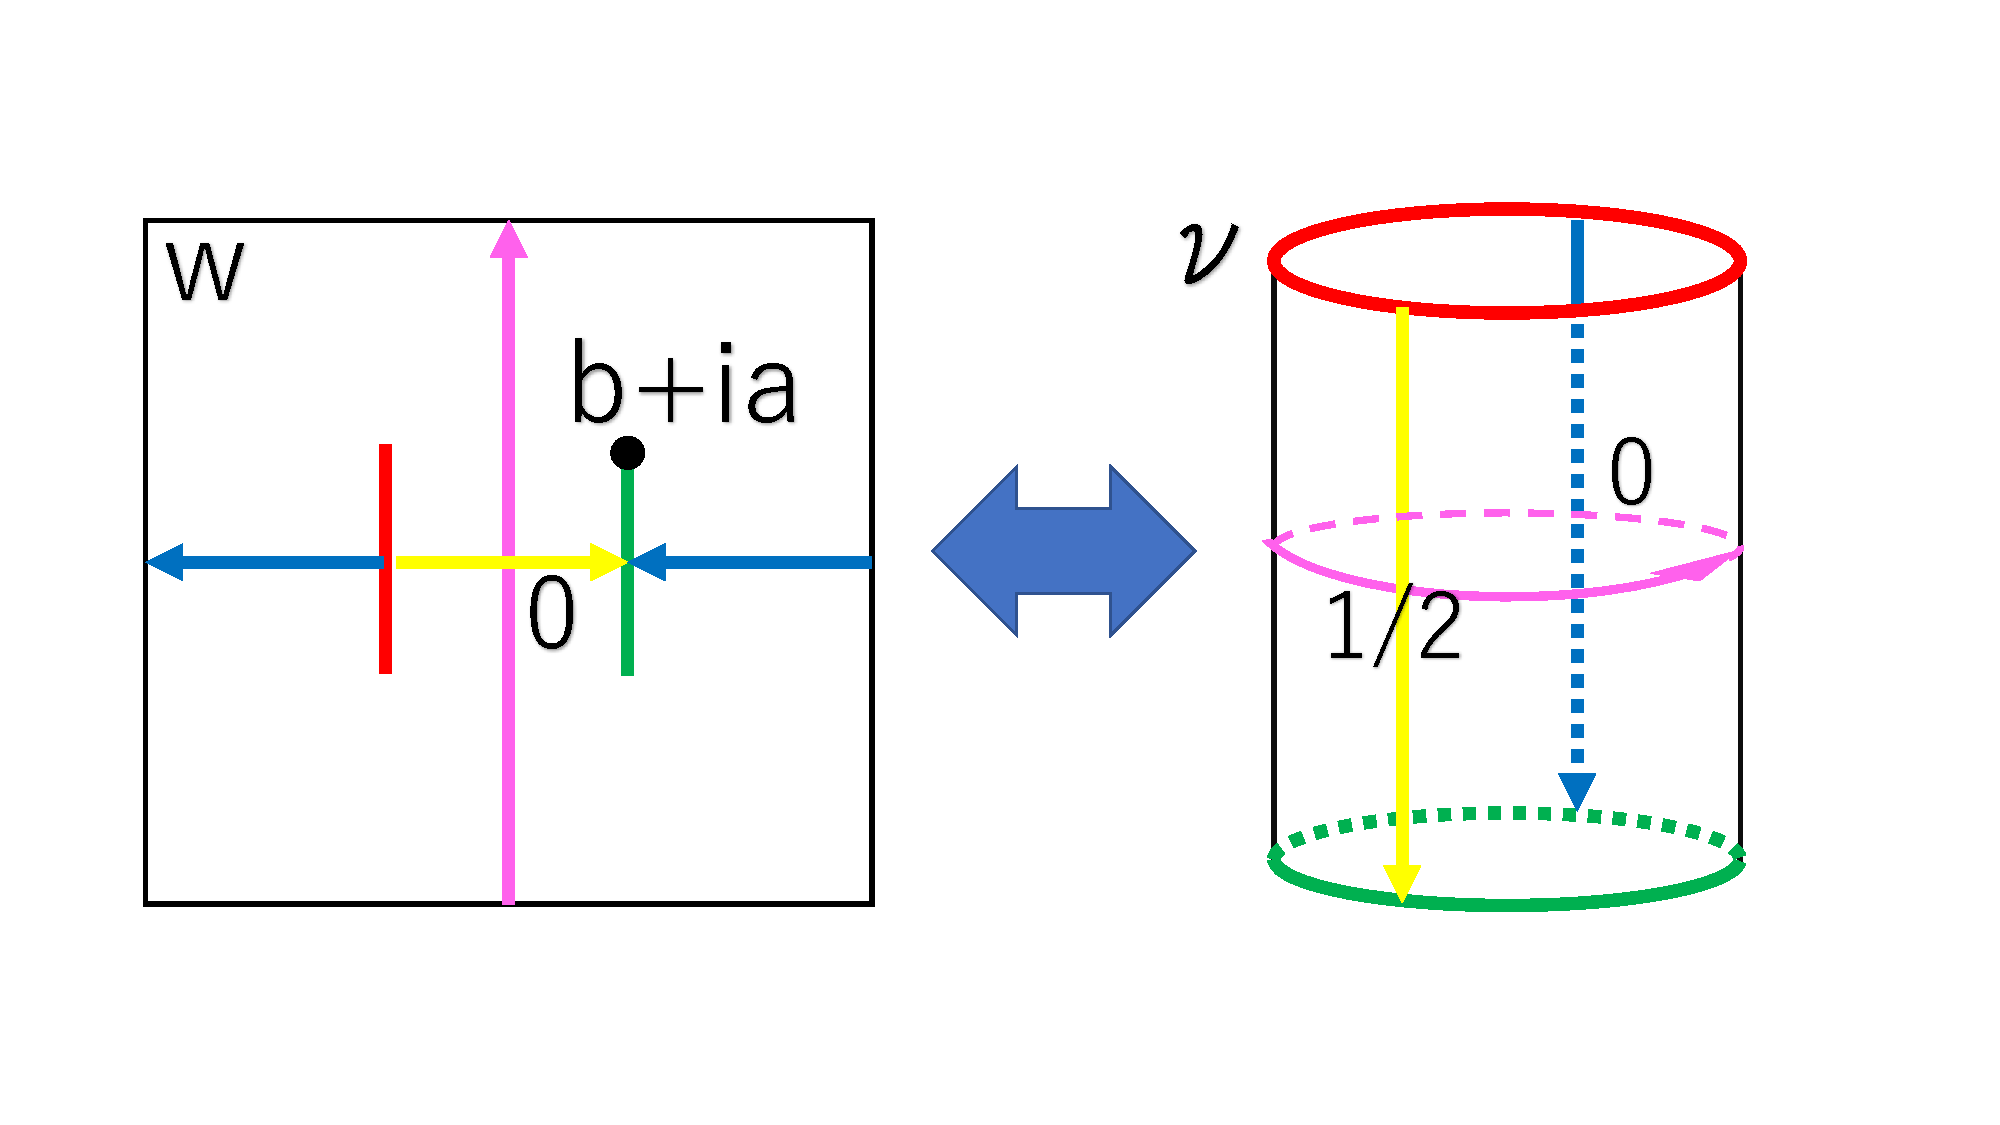
\includegraphics[width=0.7\linewidth]{DQmapping.pdf}
	\label{fig:dqmapping}
	\caption{左は2重分離クエンチされた真空についてのレプリカ法のセットアップの図。これを共形変換することで右図の有限長さの円筒に移る。}
\end{figure}

この円筒は
\begin{align}
2\pi i \beta\nu = \zeta
\end{align}
とすることで、$\RE \zeta=\pm \pi/2$に境界をもち、$\zeta\sim \zeta+2\pi i \beta$と同一視の入った円筒に移る。このとき複素共役は$\overline{w(\zeta)}=w(\overline{\zeta})$で関係づいていることに注意しておく。

パラメータ$\beta^{-1}$は$a/b$のみで決定され、その関係は次のようなグラフになる。
\begin{figure}[h]
	\centering
	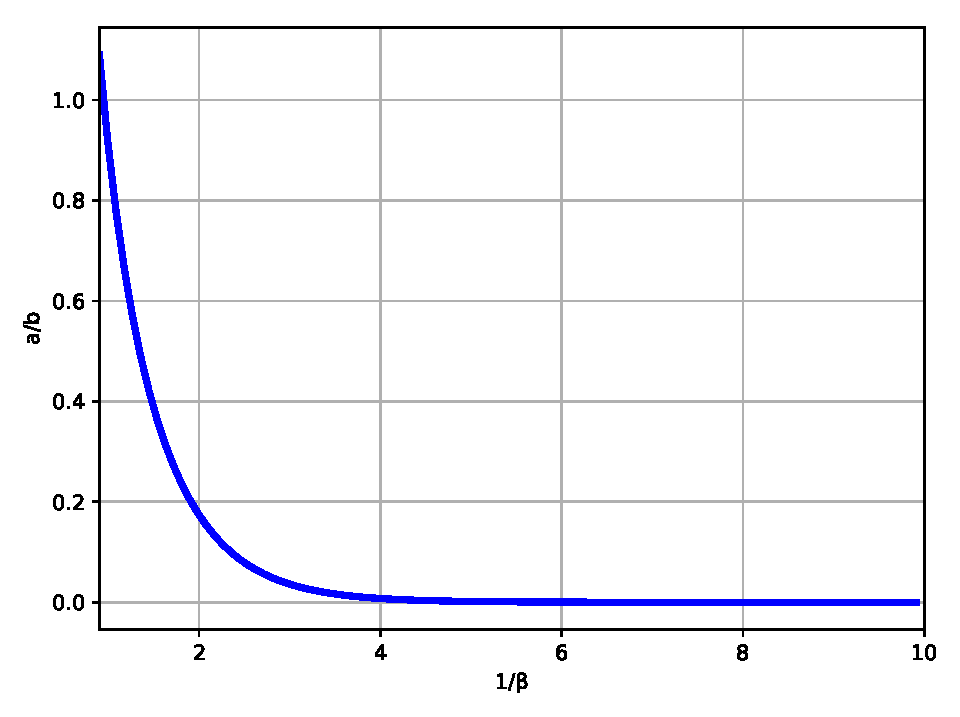
\includegraphics[width=0.5\linewidth]{s2aoverb.pdf}
	\caption{$b=50$に固定したときの、横軸が$\beta^{-1}$で縦軸が$a/b$のグラフ}
\end{figure}

$\beta^{-1}$と$a/b$の関係は、テータ関数の高温・低温極限の近似式から、$a/b\to 0,\infty$の極限で
\begin{align}
\beta^{-1}\sim \left\{ \begin{array}{ll}
\bigskip \dfrac{2b}{a} & (a/b\to \infty\iff \beta^{-1}\to 0)\\
\dfrac{2}{\pi}\log\dfrac{4b}{a} & (a/b\to 0\iff \beta^{-1}\to \infty)
\end{array}\right.
\end{align}
と近似できる。

\section{自由Dirac場}\label{sec:DSQdirac}
\subsection{EEの時間発展}
\subsub{解析計算}
$2$つの区間$[\pm b-ia,\pm b+ia]$での境界条件としてともにNeumann境界条件を課す。また、$\RE \nu$方向が$w$座標での時間方向に対応していることから、$\nu\sim \nu+1$の周期に対してNSセクターのDirac場を考える。

\ref{chap:adscftreview}章での頂点演算子の円筒$2$点関数を$\nu$座標での境界の取り方に合わせて読み替えると、零質量自由Dirac場の真空のエンタングルメントエントロピーは
\begin{align}
S_A &=\frac{1}{6}\log(\frac{G}{\epsilon^2})\\
G&=\frac{1}{(2\pi)^2}\left|\frac{dw_1}{d\nu_1}\right|\left|\frac{dw_2}{d\nu_2}\right|\notag\\
&\times \frac{\theta_1\left(\nu_1-\nu_2|i\beta^{-1}\right)\theta_1
	\left(\overline{\nu}_1-\overline{\nu}_2|i\beta^{-1}\right)\theta_1\left(\nu_1-\overline{\nu}_1+\frac{i\beta^{-1}}{2}|i\beta^{-1}\right)\theta_1\left(\nu_2-\overline{\nu}_2+\frac{i\beta^{-1}}{2}|i\beta^{-1}\right)}{\eta(i\beta^{-1})^6 \theta_1\left(\nu_1-\overline{\nu}_2+\frac{i\beta^{-1}}{2}|i\beta^{-1}\right)\theta_1
	\left(\nu_2-\overline{\nu}_1+\frac{i\beta^{-1}}{2}|i\beta^{-1}\right)}
\end{align}
となる。$2\pi i\beta \nu=\zeta$の座標変換(モジュラー変換)を用いれば、上のエンタングルメントエントロピーは\ref{fincylvertex2ptfunc}の相関関数の式をそのまま使って書くことができる。しかしいま興味のある場合は$a/b\to 0 \iff \beta\to 0$の``高温極限"の場合であるから、$\zeta$座標での相関関数を使うと数値計算でのテータ関数の収束性が悪くなる。そこで今回は$\nu$座標での相関関数を使っている。

\subsub{数値計算}
真空の寄与を引いたEE $S_A(t)-S_\text{vac}$を数値計算したものがグラフ\ref{fig:dd528}である。$b=50,a\sim 0.05\iff \beta^{-1}=5.28$で計算しており、左上図は部分系$[100,200]$、右上図は部分系$[10,30]$、左下図は部分系$[30,100]$、右下図は$[-150,100]$にとった場合である。
\begin{figure}[H]
	\centering
	\begin{tabular}{c}
		\begin{minipage}{0.50\hsize}
			\centering
			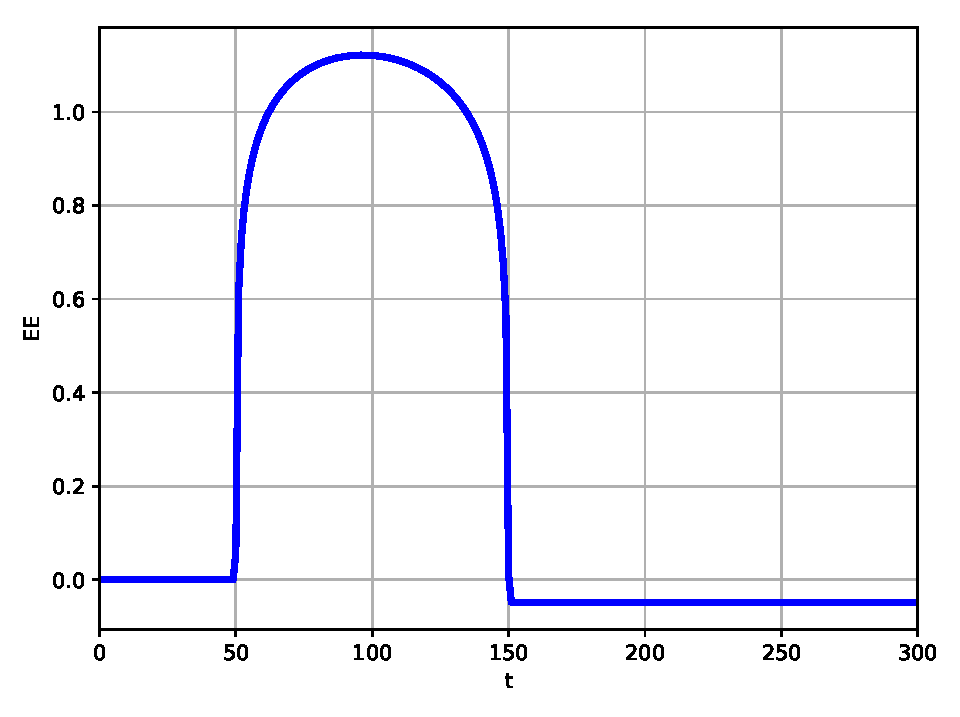
\includegraphics[width=\linewidth]{dd528_100_200.pdf}
		\end{minipage}
		\begin{minipage}{0.50\hsize}
			\centering
			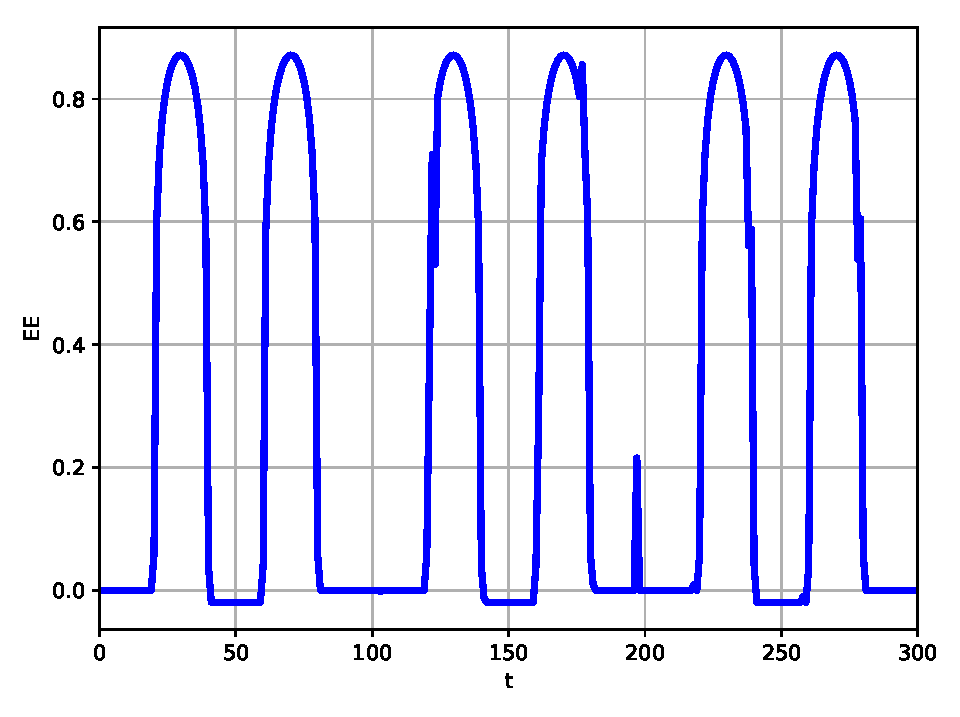
\includegraphics[width=\linewidth]{dd528_10_30.pdf}
		\end{minipage}
		\begin{minipage}{0.06\hsize}
			\vspace{10mm}
		\end{minipage} \\
		\begin{minipage}{0.50\hsize}
			\centering
			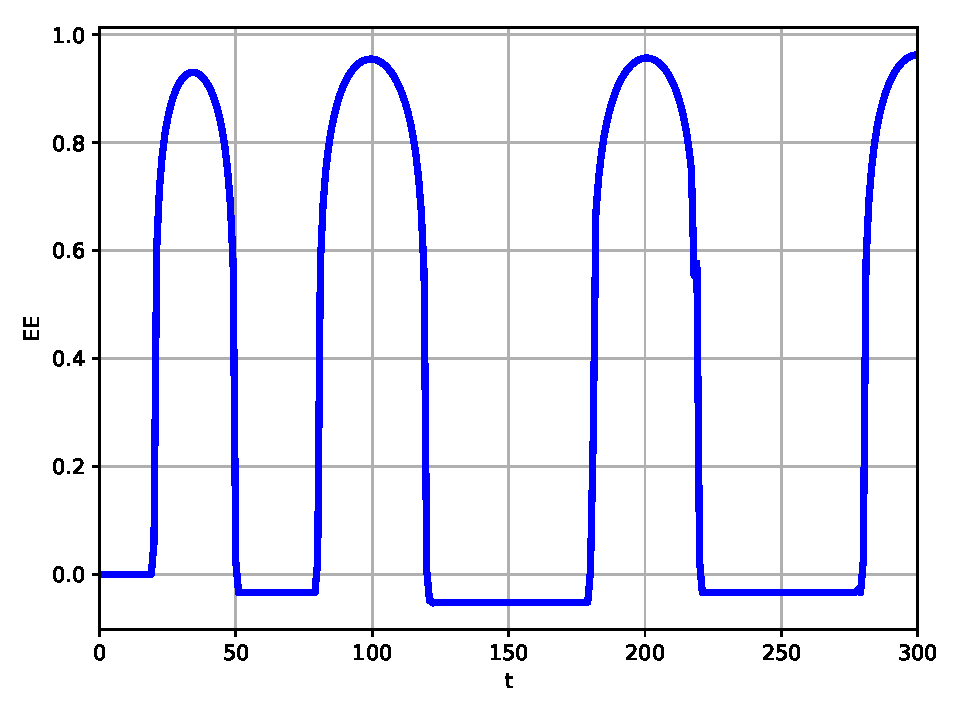
\includegraphics[width=\linewidth]{dd528_30_100.pdf}
		\end{minipage}
		\begin{minipage}{0.50\hsize}
			\centering
			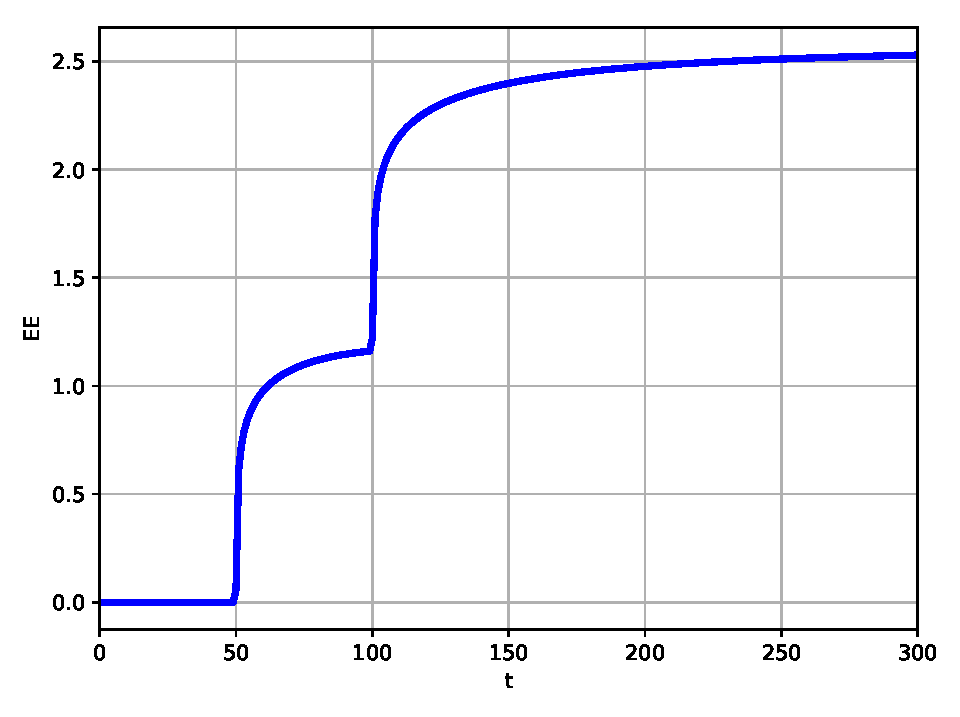
\includegraphics[width=\linewidth]{dd528_150_100.pdf}
		\end{minipage}
	\end{tabular}
	\caption{自由Dirac場の真空を$b=50,a\sim 0.05$で2重分離クエンチしたときのEEのグラフ。横軸は時間$t$で、縦軸は真空の寄与を引いたEE $S_A(t)-S_\text{vac}$をプロットしている。}
	\label{fig:dd528}
\end{figure}

次に$b=50,a\sim 50 \iff \beta^{-1}=0.945$で計算した結果をグラフ\ref{fig:dd0945}にあげる。部分系の取り方は同様で、左上図は部分系$[100,200]$、右上図は部分系$[10,30]$、左下図は部分系$[30,100]$、右下図は$[-150,100]$にとった場合である。
\begin{figure}[H]
	\centering
	\begin{tabular}{c}
		\begin{minipage}{0.50\hsize}
			\centering
			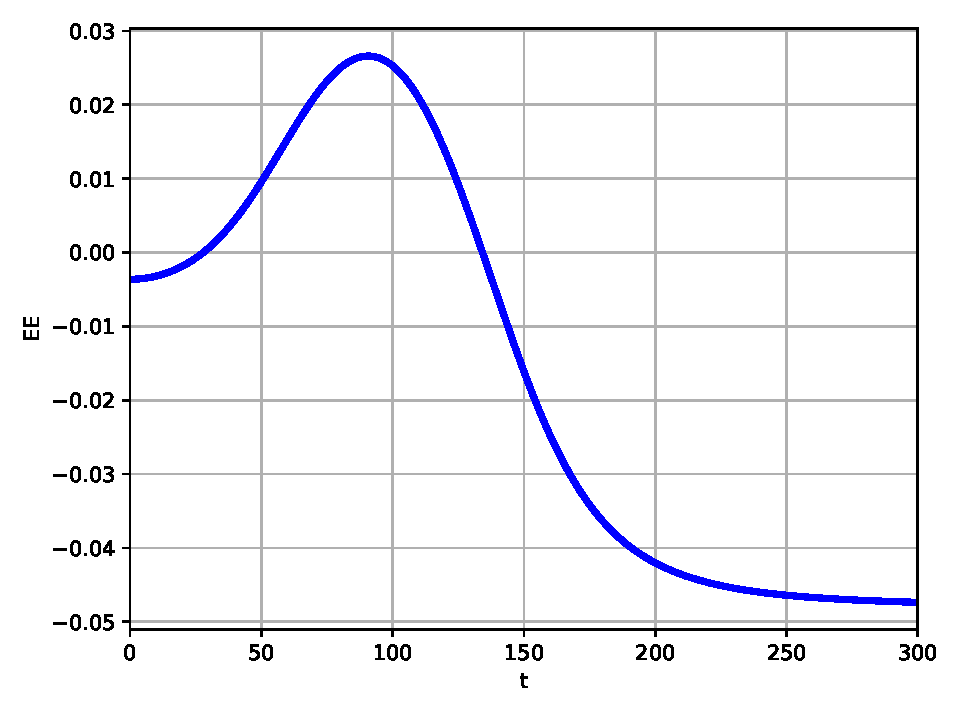
\includegraphics[width=\linewidth]{dd0945_100_200.pdf}
		\end{minipage}
		\begin{minipage}{0.50\hsize}
			\centering
			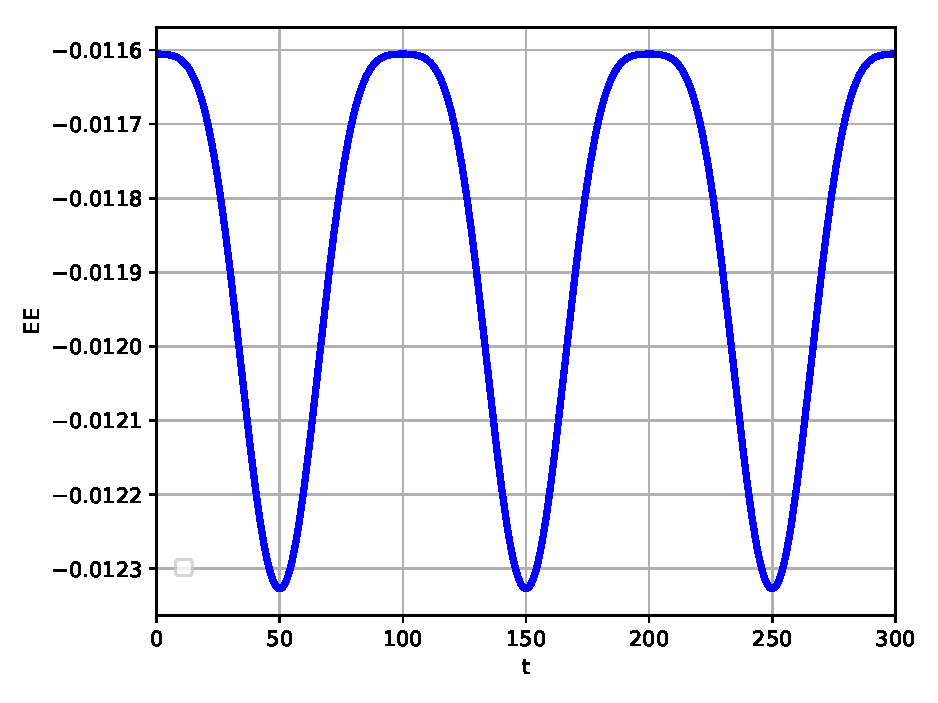
\includegraphics[width=\linewidth]{dd0945_10_30.pdf}
		\end{minipage}
		\begin{minipage}{0.06\hsize}
			\vspace{10mm}
		\end{minipage} \\
		\begin{minipage}{0.50\hsize}
			\centering
			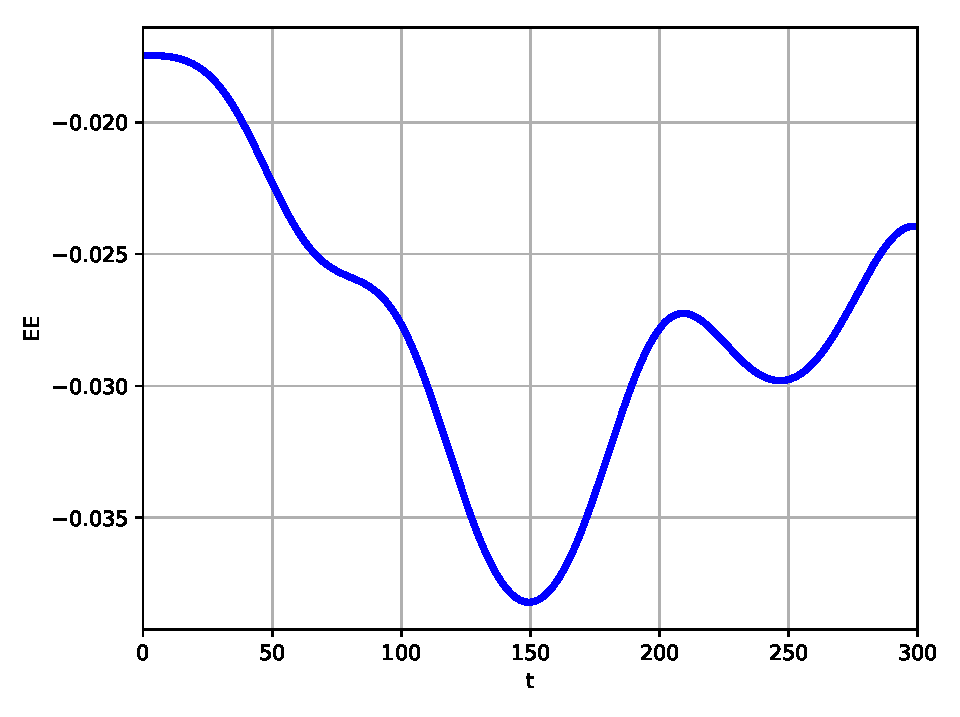
\includegraphics[width=\linewidth]{dd0945_30_100.pdf}
		\end{minipage}
		\begin{minipage}{0.50\hsize}
			\centering
			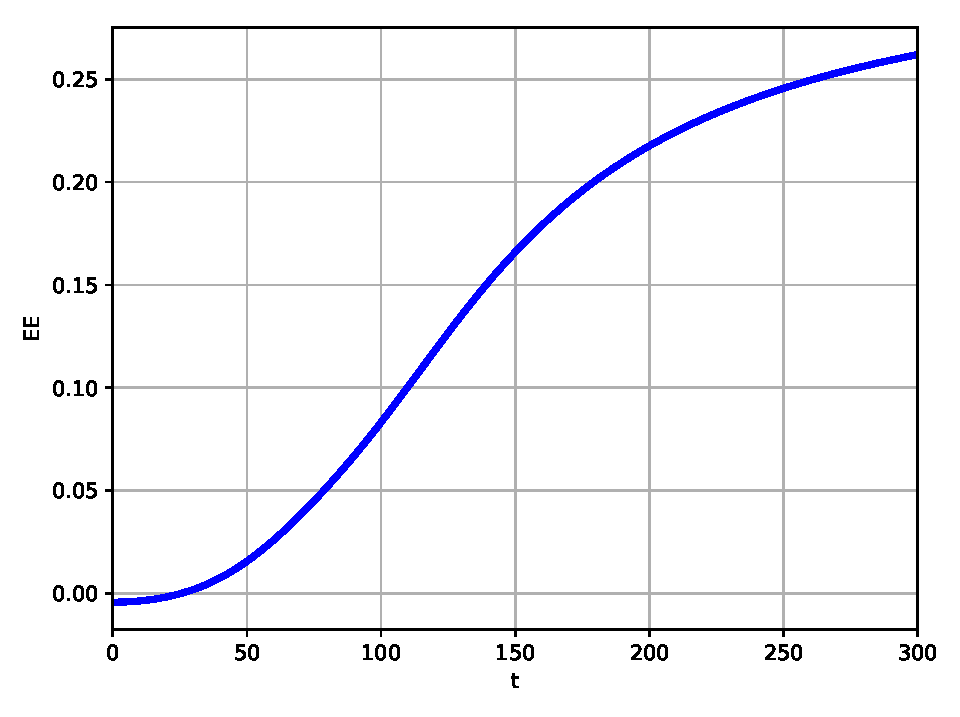
\includegraphics[width=\linewidth]{dd0945_150_100.pdf}
		\end{minipage}
	\end{tabular}
	\caption{自由Dirac場の真空を$b=50,a\sim 50$で2重分離クエンチしたときのEEのグラフ。横軸は時間$t$で、縦軸は真空の寄与を引いたEE $S_A(t)-S_\text{vac}$をプロットしている。}
	\label{fig:dd0945}
\end{figure}
いずれの結果も右下の図を除いて、準粒子描像に当てはまっていることが分かる。

\subsection{中央の領域の熱力学的エントロピー}
\subsub{中央の領域の熱力学的エントロピー}
2重分離クエンチを考えると空間領域は$L,C,R$の$3$つに分かれる。円筒分配関数\ref{diracPFfincyl}から中央の領域の$t\to\infty$における熱力学的エントロピーを求める。エンタングルメントエントロピーの計算に用いたのは$\nu$座標での相関関数だったから、
\begin{align}
\log Z(\beta) &= \log \frac{\theta_3(0|i\beta^{-1})}{\eta(i\beta^{-1})}\\ &=\frac{\pi\beta^{-1}}{12}+2\sum_{m=1}^{\infty}\log (1+e^{-2\pi(m-\frac{1}{2})\beta^{-1}})
\end{align}
であることに注意すると、熱力学的エントロピーは
\begin{align}
S_\text{thermal}&=-\frac{\del \left(-(2\pi\beta)^{-1}\log Z(\beta)\right)}{\del (2\pi\beta)^{-1}}\\
&=\frac{1}{6}\pi\beta^{-1}+2\sum_{m=1}^{\infty} \log(1+e^{-2\pi (m-1/2)\beta^{-1}})-4\pi\beta^{-1}\sum_{m=1}^{\infty}\frac{m-1/2}{1+e^{2\pi (m-1/2)\beta^{-1}}}
\end{align}
となる。さらに$\beta\to 0$の高温極限で熱力学的エントロピーは
\begin{align}
S_\text{thermal}\sim \frac{1}{6}\pi\beta^{-1}\sim \frac{1}{3}\log\frac{4b}{a}
\end{align}
となる。これはBTZブラックホールのエントロピー$\frac{c}{3}\pi\beta^{-1}$を$1/2$倍したものと同じ形をしていることに注意しておく。また、$\beta\to 0$の極限は$b\gg a$の極限に等価である。したがって$S_\text{thermal}$は$a/2$を紫外カットオフと思ったときの領域$C$の真空のエンタングルメントエントロピーに一致することにも注意しておく。

\subsub{領域$L,R$に端点をもち、$C$にまたがるような大きな部分系$A$のEE}
部分系$A=[-X,X],\ X\gg b$のEEについて考える。部分系$A$を$(A\intersection L)\union C \union (A\intersection R)$と3つの因果的に独立な領域に分けると、領域$(A\intersection L),(A\intersection R)$は領域$C$に比べて非常に大きい。このとき領域$C$で起きたクエンチの情報は粗視化されてしまい、$C$は内部の情報にアクセスできなくなった領域として振る舞うようになると考えられる。また、領域$C$が小さい場合を考えるので、$a/b$も小さくなる($\iff$ 高温極限$\beta\to 0$)。したがって、$A$のEEは
\begin{align}
S_A&\sim (A\text{の真空のEE})+(C\text{の熱力学的エントロピー})\\
&=\frac{1}{3}\log\frac{2X}{\epsilon}+\frac{1}{6}\pi\beta^{-1}\label{thermalization}
\end{align}
となると推測される。

実際これが成り立つことを、数値計算で確かめてみる。$b=50,a\sim 0.05\iff \beta^{-1}=5.28$として、部分系$A=[-X,X]$の端点$X$を$100\le X \le 10000$まで変化させ、それぞれの系に対して$t=10^6$でのEE $S_A(t)-S_\text{vac}$を数値計算したものが図\ref{fig:cthermalization}である。
\begin{figure}[H]
	\centering
	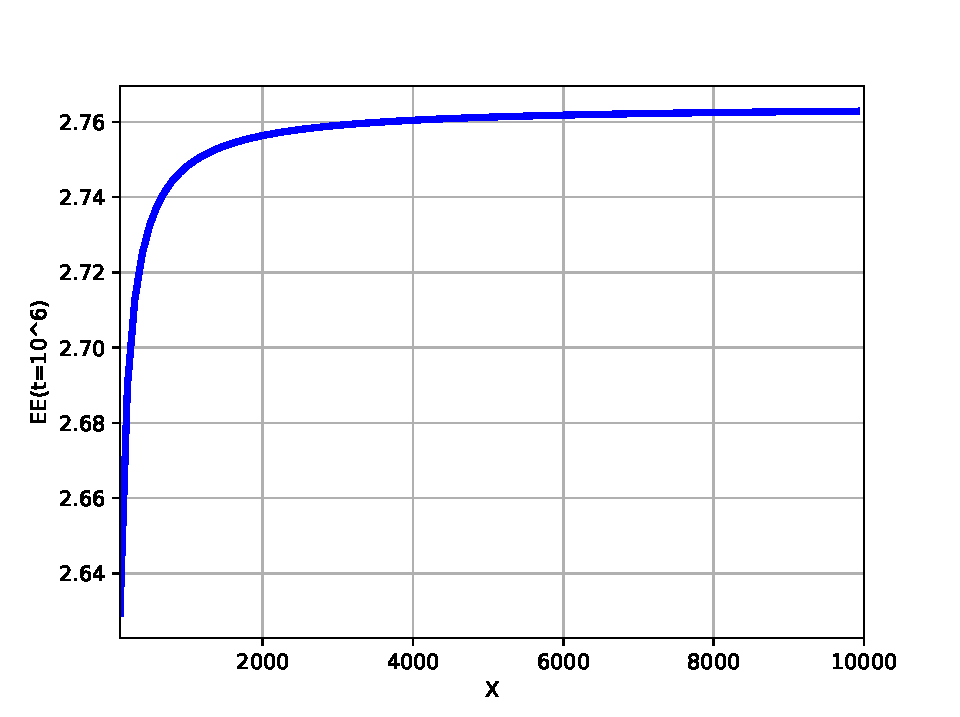
\includegraphics[width=0.7\linewidth]{Cthermalization.pdf}
	\caption{自由Dirac場の真空を$b=50,a\sim 0.05\iff \beta^{-1}=5.28$で2重分離クエンチしたときの、時刻$t=10^6$でのEEのグラフ。横軸は部分系の大きさ$X$で、縦軸は真空の寄与を引いたEE $S_A(t=10^6)-S_\text{vac}$をプロットしている。}
	\label{fig:cthermalization}
\end{figure}

このときたしかに$X\gg b$の``熱力学極限''で、真空の寄与を引いたEE $S_A(t)-S_\text{vac}$が領域$C$の熱力学的エントロピー
\begin{align}
S_\text{thermal}\sim \frac{1}{6}\pi\beta^{-1}\sim 2.76460\cdots
\end{align}
に漸近していて、(\ref{thermalization})が成立している。
\pagebreak
\section{重力双対をもつ共形場理論}\label{sec:DSQholcft}
重力双対をもつ、有限長さの円筒上の共形場理論に双対となるAdS空間を考えたい。

AdS/BCFTでNeumann境界条件を課せば、トーラスを境界に持つAdS空間であるthermal AdSやthermal non-rotating BTZが双対なAdS空間となる。どちらが双対な時空となるかはCFTの逆温度$\beta$で決まり、
\begin{align}
\beta<1 &\to \text{thermal non-rotating BTZ black hole}\\
\beta>1 &\to \text{thermal AdS}
\end{align}
で対応している。以下ではこの2つの場合に分けてエンタングルメントエントロピーを計算する。

\subsection{thermal non-rotating BTZ ($\beta<1$)の場合}
\subsub{解析計算}
$2\pi i \beta \nu=\zeta=X+i T$とすれば、$\zeta$座標の円筒にその鏡像を加えて得られるトーラスは
\begin{align}
X\sim X+2\pi,\ T\sim T+2\pi\beta
\end{align}
の同一視で作られる。(\ref{BTZblackbrane})より、このCFTに対応するthermal non-rotating BTZ計量は
\begin{align}
ds^2=\frac{R_A^2}{z^2}\left( \frac{dz^2}{1-z^2/\beta^2}+\left(1-z^2/\beta^2\right)dT^2+dX^2 \right)
\end{align}
となる。
\begin{figure}[h]
	\centering
	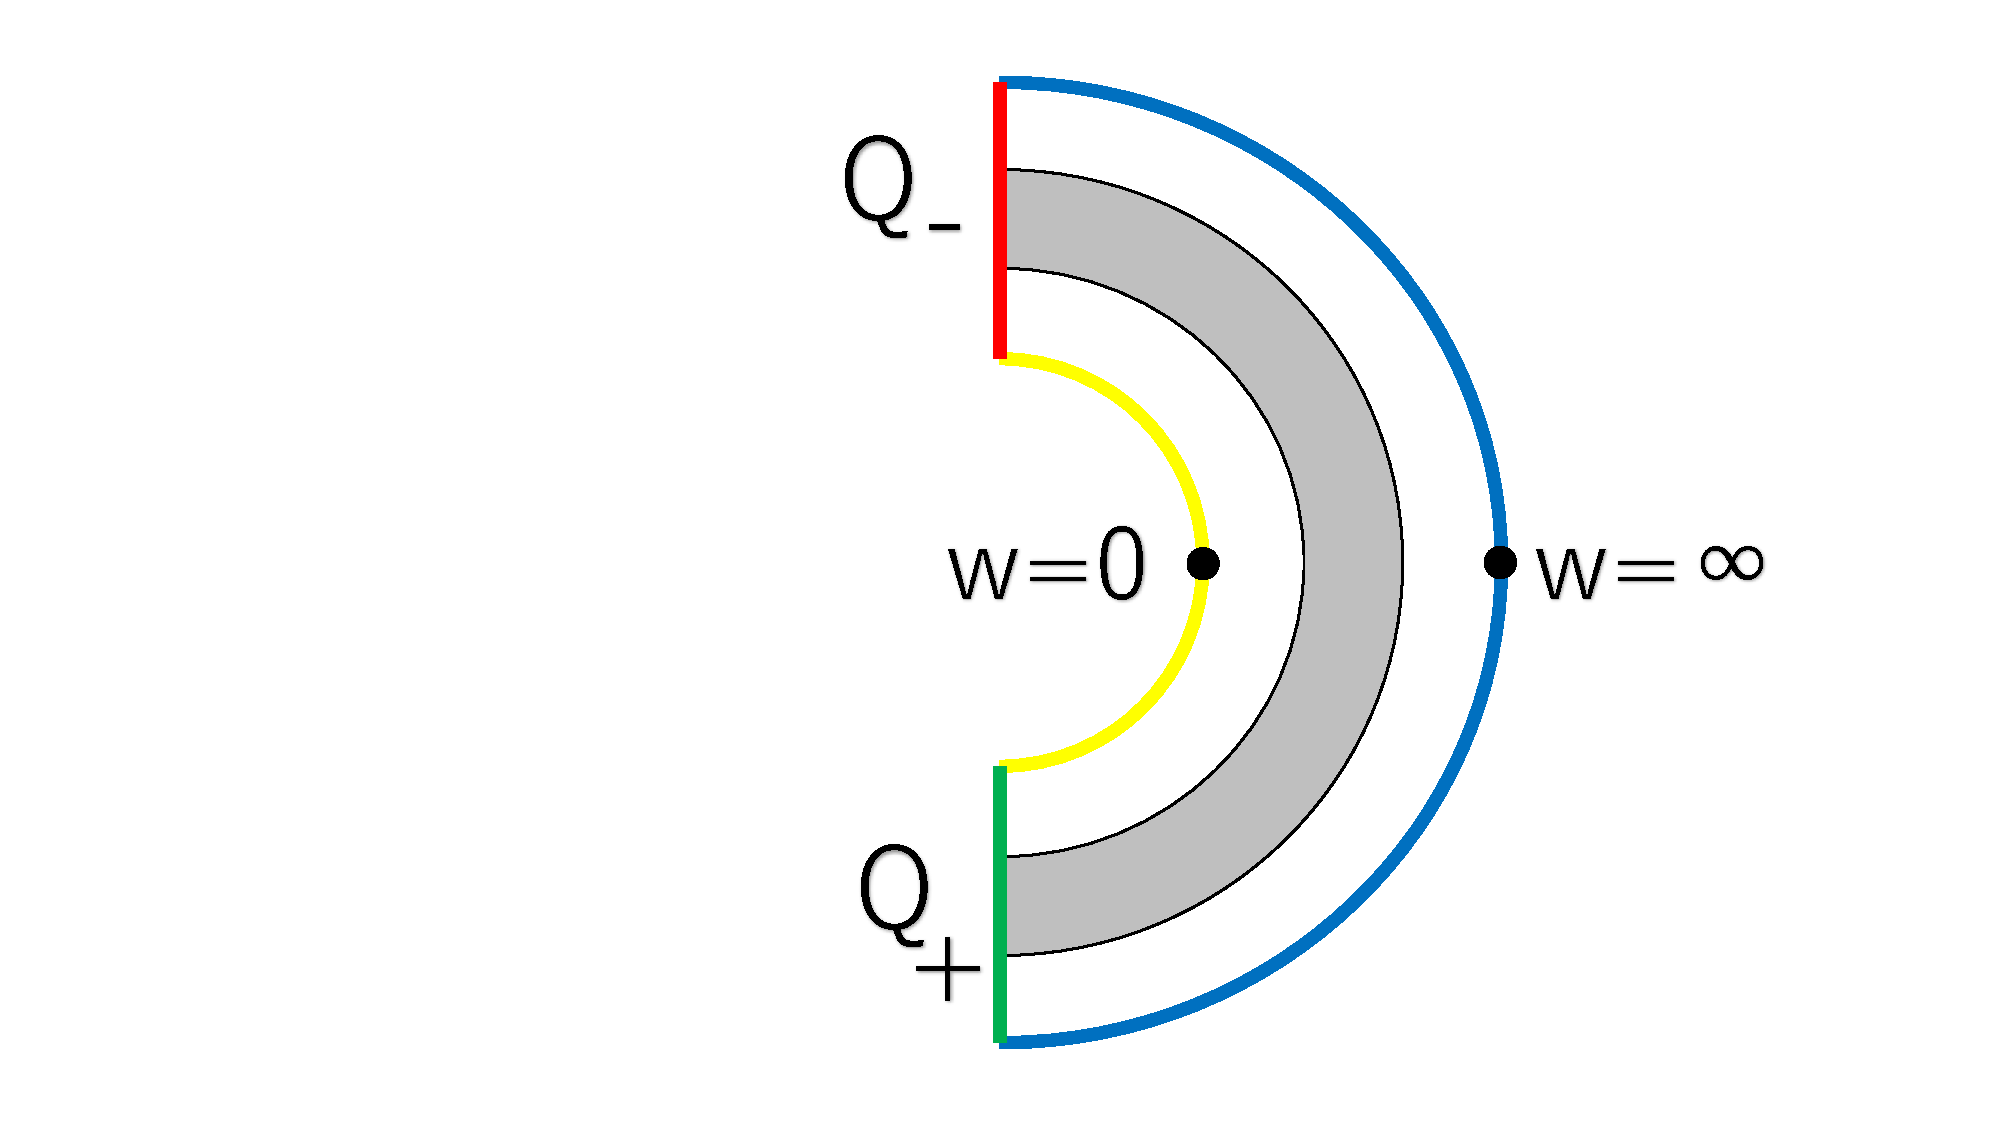
\includegraphics[width=0.7\linewidth]{DQads.pdf}
	\caption{双対なBTZ時空の$\tau=0$の図。この面で測地線を見つければよい。}
	\label{fig:dqads}
\end{figure}

いま、$w$座標での区間$A=[x_1,x_2]$の真空のエンタングルメントエントロピーを笠-高柳公式から求める。$w_i=x_i+i\tau_i\ (i=1,2)$に対応する$\nu,\zeta$座標の点を$\nu_i,\zeta_i$とする。

$c\gg 1$近似を使えば、エンタングルメントエントロピーは
\begin{align}
S_A=\min\{ S_A^{con},S_A^{dis} \}
\end{align}
として求まる。ただし$S_A^{con}$は$\zeta_1,\zeta_2$を結ぶ測地線の長さで決まる。non-rotating BTZ空間の境界の$2$点間の測地線の長さは(\ref{geodlengthGlobal})において$L=\beta^{-1}$として$\sin$を$\sinh$と読み替えればよいから、$S_A^{con}$は
\begin{align}
S^{con}_A&=\frac{c}{6}\log \left( \frac{4\beta^2}{\delta_1\delta_2}\sinh\left(\frac{\zeta_1-\zeta_2}{2\beta} \right)\sinh\left(\frac{\overline{\zeta}_1-\overline{\zeta}_2}{2\beta} \right) \right)\\
&=\frac{c}{6}\log \left( \left(\frac{1}{\pi\epsilon}\right)^2\left|\frac{dw_1}{d\nu_1}\right|\left|\frac{dw_2}{d\nu_2}\right|\sin\left(\pi (\nu_1-\nu_2) \right)\sin\left(\pi (\overline{\nu}_1-\overline{\nu}_2) \right) \right)
\end{align}
となる。ただし$\delta_i (i=1,2)$は\ref{cutofftransf}と同様に、
\begin{align}
\epsilon = \frac{1}{2\pi\beta}\left|\frac{dw_i}{d\nu_i}\right| \delta_i
\end{align}
で関係している。

また$S_A^{dis}$は$\zeta_1,\zeta_2$とそれぞれの鏡像点を結ぶ測地線の長さとして決まる。ただし今の場合、boundary surfaceが2つあるので、ホモロジー条件に注意する必要がある。BCFTの境界$[-b-ia,-b+ia],[b-ia,b+ia]$に対応するboundary surfaceをそれぞれ$Q_-,Q_+$を呼ぶことにする。$\zeta_1,\zeta_2$が共に$Q_+$にエンドする場合や、共に$Q_-$にエンドする場合にはそのまま測地線の長さがエントロピーになる。しかし$\zeta_1,\zeta_2$がそれぞれ別の$Q_{\pm}$にエンドする場合、ホモロジー条件からBTZ BHのエントロピーの半分だけ新たに寄与が生じる。
\begin{figure}[h]
	\centering
	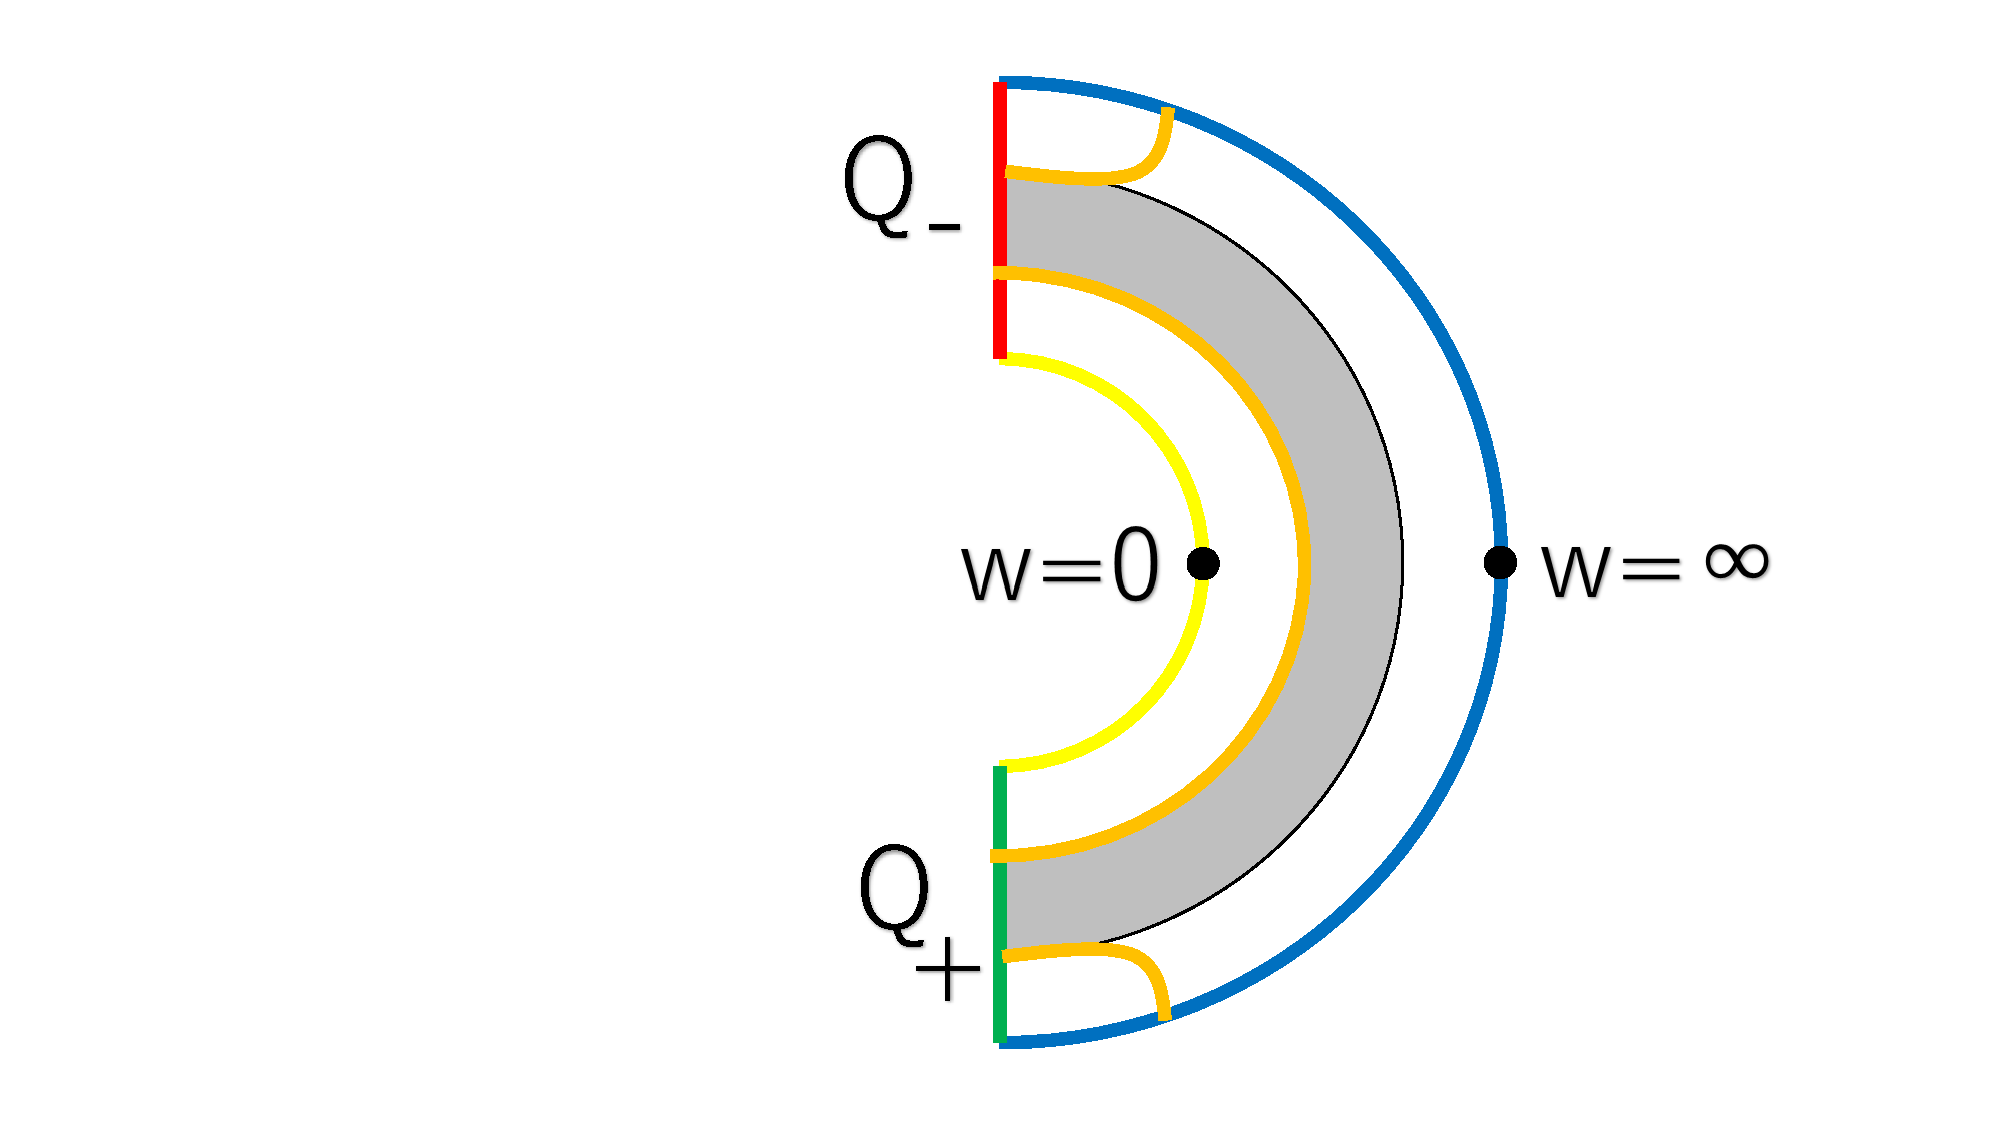
\includegraphics[width=0.7\linewidth]{DQadsgeod.pdf}
	\caption{たとえば連結区間$A=[x_1,x_2],\ x_1\lesssim -b<b\lesssim x_2$についてのEEを考える。これに双対なAdSのセットアップを考えると中央の領域と外側の領域が離れたところにある。このときホモロジー条件により中央の領域の部分からブラックホールエントロピーの半分の値が現れる。}
	\label{fig:dqadsgeod}
\end{figure}

つまり$S_A^{dis}$は以下の式で求められる。

\begin{align}
S_A^{dis}=\min_{\sigma_1=\pm 1,\sigma_2=\pm 1}&\left( \frac{c}{6}\log \frac{1}{\pi\epsilon}\left|\frac{dw_1}{d\nu_1}\right| \sin\left(\pi(\nu_1-\overline{\nu}_1+\frac{i \sigma_1\beta^{-1}}{2})\right)+(1\leftrightarrow 2)\right.\notag\\
&\left.+\frac{1-\sigma_1\sigma_2}{2}\times \frac{c}{6}\pi\beta^{-1}\right)
\end{align}

\subsub{数値計算}
上の計算を数値計算したものがグラフ\ref{fig:dh528}である。$b=50,a=0.05$で計算しており、左上図は部分系$[100,200]$、右上図は部分系$[10,30]$、左下図は部分系$[30,100]$、右下図は$[-150,100]$にとった場合である。
\begin{figure}[H]
	\centering
	\begin{tabular}{c}
		\begin{minipage}{0.50\hsize}
			\centering
			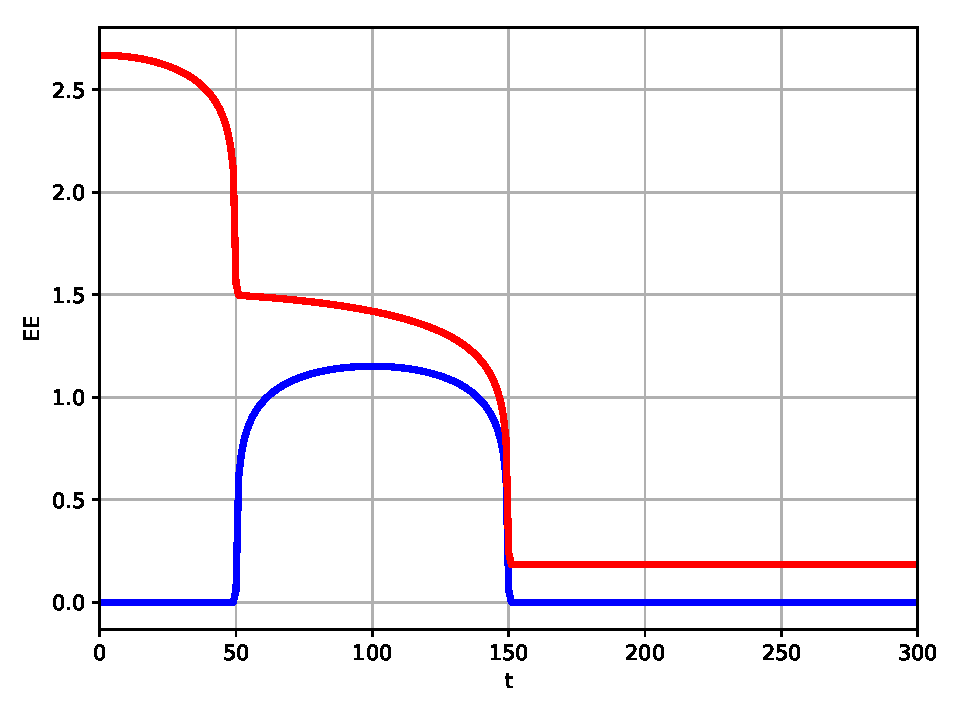
\includegraphics[width=\linewidth]{dh528_100_200.pdf}
		\end{minipage}
		\begin{minipage}{0.50\hsize}
			\centering
			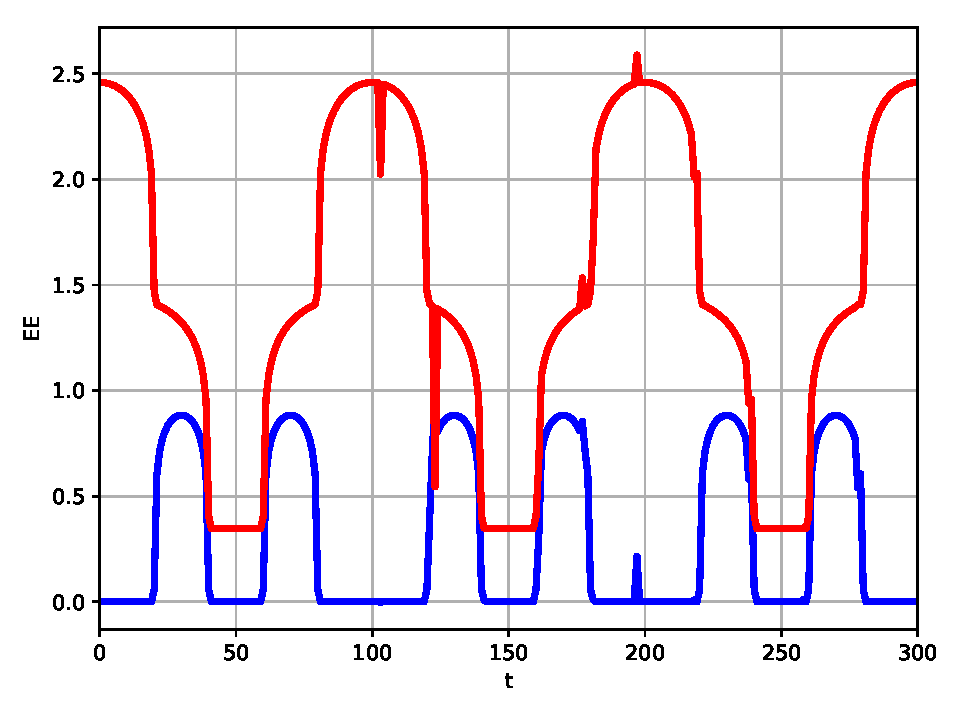
\includegraphics[width=\linewidth]{dh528_10_30.pdf}
		\end{minipage}
		\begin{minipage}{0.06\hsize}
			\vspace{10mm}
		\end{minipage} \\
		\begin{minipage}{0.50\hsize}
			\centering
			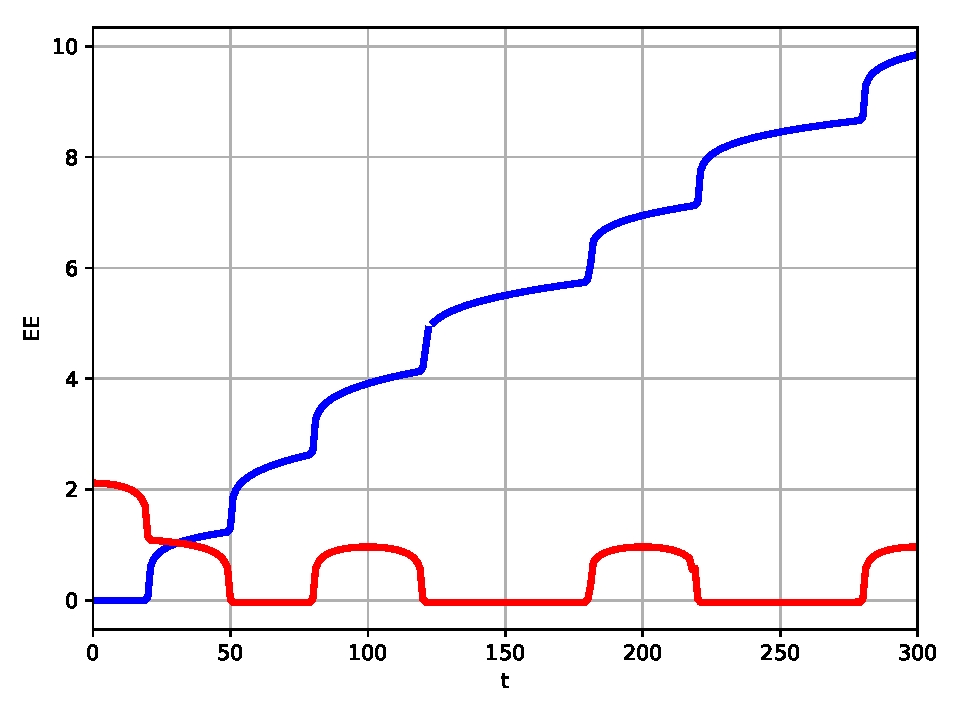
\includegraphics[width=\linewidth]{dh528_30_100.pdf}
		\end{minipage}
		\begin{minipage}{0.50\hsize}
			\centering
			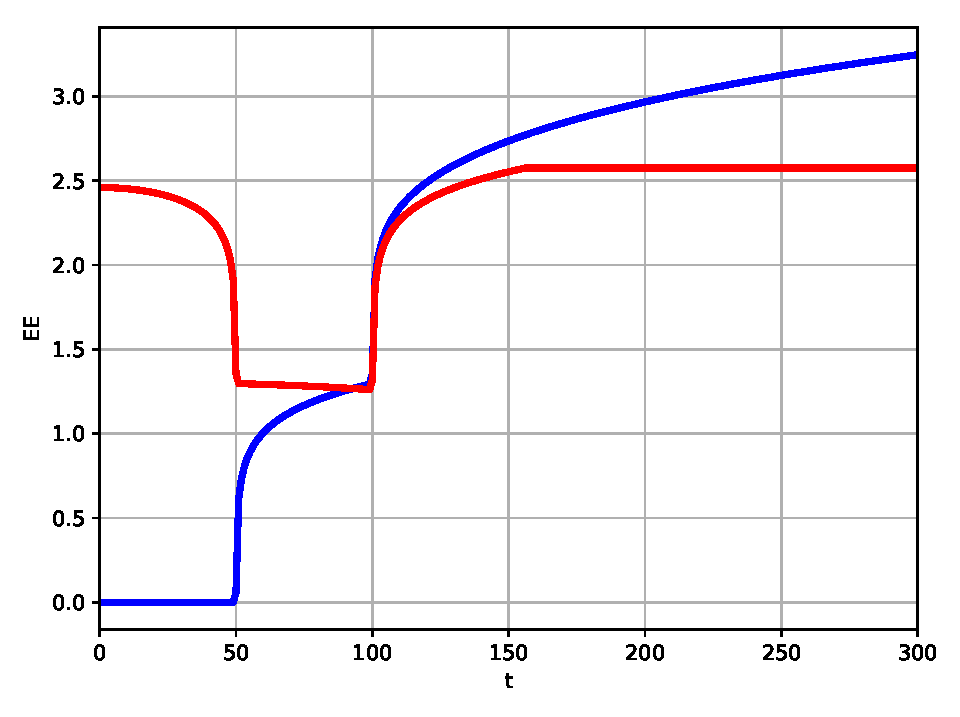
\includegraphics[width=\linewidth]{dh528_150_100.pdf}
		\end{minipage}
	\end{tabular}
	\caption{重力双対を持つ共形場理論の真空を$b=50,a=0.05$で2重分離クエンチしたときのEEのグラフ。横軸は時間$t$で、縦軸は真空の寄与を引いたEE $S_A(t)-S_\text{vac}$をプロットしている。}
	\label{fig:dh528}
\end{figure}
この結果から、右下の図を除いて準粒子描像に当てはまっていることが分かる。

\subsub{BTZ相での、中央の領域$C$を囲む領域のEE}
中央の領域$C$を覆う領域$A,\ (C\subset A)$に対する$S_A(t)-S_\text{vac}$はDirac場の時とは異なり、$t\to\infty$極限をとらなくてもエントロピーはある値に到達した後で一定値になる。これは重力双対をもつような共形場理論がDirac場に比べて非常にカオス性が強く、情報が瞬時に粗視化されてしまうことが表れている。とくに熱力学極限をとればその一定値は、Dirac場と同様に
\begin{align}
S_C(t\gg b)-S_\text{vac} \sim \frac{c}{6}\pi\beta^{-1} \sim \frac{c}{3}\log\frac{4b}{a}
\end{align}
となる。重力双対をもつ共形場理論の場合でも、$C$の熱力学的エントロピーは$a/2$を紫外カットオフと思った領域$C$のエンタングルメントエントロピーに一致している。

\subsection{thermal AdS ($\beta>1$)の場合}
\subsub{解析計算}
逆温度$\beta$のthermal AdSは逆温度$\beta^{-1}$のthermal non-rotating BTZに等しいことに注意すると、$\zeta$座標のCFTに対するthermal AdSの計量は
\begin{align}
ds^2&=\frac{1}{z^2}\left( \frac{dz^2}{1-\beta^2z^2}+\left(1-\beta^2z^2\right)dX^2+dT^2 \right)\\
X&\sim X+2\pi/\beta,\ T\sim T+2\pi
\end{align}
となる。

したがってThermal AdS相での$S_A^{con}$は
\begin{align}
S^{con}_A&=\frac{c}{6}\log \left( \frac{4}{\beta^2\delta_1\delta_2}\sinh\left(\frac{\beta(\zeta_1-\zeta_2)}{2} \right)\sinh\left(\frac{\beta(\overline{\zeta}_1-\overline{\zeta}_2)}{2} \right) \right)\\
&=\frac{c}{6}\log \left( \left(\frac{1}{\pi\beta\epsilon}\right)^2\left|\frac{dw_{1}}{d\nu_{1}}\right|\left|\frac{dw_{2}}{d\nu_{2}}\right|\sin\left(\pi\beta (\nu_1-\nu_2) \right)\sin\left(\pi\beta (\overline{\nu}_1-\overline{\nu}_2) \right)\right)
\end{align}
また$S^{dis}_A$は
\begin{equation}
S^{dis}_A=\min_{\sigma_1,\sigma_2=\pm 1}\left[\frac{c}{6}\log \left( \frac{1}{\pi\beta\epsilon}\left|\frac{dw_{1}}{d\nu_{1}}\right|\sinh\left(\pi\beta\left(\nu_1-\overline{\nu}_1+ \sigma_1 \frac{i}{2\beta}\right)\right)\right)+(1\leftrightarrow 2)\right]
\end{equation}
で計算される。

\subsub{数値計算}
$b=50,a=50$で計算した結果をグラフ\ref{fig:dh0945}にあげる。部分系の取り方は同様で、左上図は部分系$[100,200]$、右上図は部分系$[10,30]$、左下図は部分系$[30,100]$、右下図は$[-150,100]$にとった場合である。
\begin{figure}[H]
	\centering
	\begin{tabular}{c}
		\begin{minipage}{0.50\hsize}
			\centering
			\includegraphics[width=\linewidth]{dh0945_100_200.pdf}
		\end{minipage}
		\begin{minipage}{0.50\hsize}
			\centering
			\includegraphics[width=\linewidth]{dh0945_10_30.pdf}
		\end{minipage}
		\begin{minipage}{0.06\hsize}
			\vspace{10mm}
		\end{minipage} \\
		\begin{minipage}{0.50\hsize}
			\centering
			\includegraphics[width=\linewidth]{dh0945_30_100.pdf}
		\end{minipage}
		\begin{minipage}{0.50\hsize}
			\centering
			\includegraphics[width=\linewidth]{dh0945_150_100.pdf}
		\end{minipage}
	\end{tabular}
	\caption{重力双対を持つ共形場理論の真空を$b=50,a=50$で2重分離クエンチしたときのEE}
	\label{fig:dh0945}
\end{figure}
この結果から、右下の図を除いて準粒子描像に当てはまっていることが分かる。


\section{2つの1重分離クエンチと2重分離クエンチの比較と重力相互作用}\label{sec:DSQSPQ}

3次元AdS重力はChern-Simons理論だったので、その内部領域には力学的自由度が無い。しかし境界には力学的自由度が存在し、これはboundary gravitonと呼ばれている。

1重クエンチの解析で、共形場理論の境界の双対は、AdS空間での重い物体であることが分かった。我々の2重クエンチのモデルにおいても同様のことが成り立つと考えられるが、このときboundary gravitonによって2つの重い物体同士は引き合うと考えられる。
\begin{figure}[h]
	\centering
	\includegraphics[width=0.7\linewidth]{DQgravdual.pdf}
	\caption{点線が重力相互作用が無いと仮定した場合の境界・測地線の図で、実線が今回のセットアップの図である。}
	\label{fig:dqgravdual}
\end{figure}
このとき笠-高柳公式を考えると、クエンチ点から離れたところの測地線を2重クエンチの場合と、2つの独立な1重クエンチで比較したときに、前者のほうが計量のゆがみが減ることにより短くなると考えられる。そこで次の予想を立てた。
\begin{align}\label{conjecture}
S^\text{double}-(S^{\text{single, }+b}+S^{\text{single, }-b})<S_\text{vac}
\end{align}
ただし$S_\text{vac}=\frac{c}{3}\log\frac{L}{\epsilon}$は真空のエンタングルメントエントロピーを表している。

たとえば$b=50,a=1$で部分系$A=[100,200]$に対して比
\begin{align}
R=\frac{S^\text{double}-S_\text{vac}}{S^{\text{single, }+b}+S^{\text{single, }-b}-2S_\text{vac}}
\end{align}
を計算してみるとグラフのようになり、確かに上の不等式は成り立っている。
\begin{figure}[h]
	\centering
	\includegraphics[width=0.7\linewidth]{DSratio.pdf}
	\caption{各時刻$t$での比$R$の値。$R<1$なら\ref{conjecture}が成立している。}
	\label{fig:dsratio}
\end{figure}

$b\ll x_1,x_2$となるような部分系$A=[x_1,x_2]$に対しては、boundary gravitonの存在によって、つねに上の不等式が成り立つと我々は予想している。
	\chapter{まとめと今後の展望}
\section*{まとめ}
本論文では、AdS/CFT対応の手法を利用した分離クエンチにおけるエンタングルメントのダイナミクスの解析を述べた。

\ref{chap:adscftreview}章ではAdS$_3$/CFT$_2$対応を概説した。AdS$_3$/CFT$_2$対応では、2次元共形場理論のVirasoro対称性が3次元漸近的AdS時空の境界にあるVirasoro対称性に対応し、さらに共形場理論の高温/低温状態はブラックホールが存在する/しない時空に対応する。そして共形場理論の高温状態のエントロピーはCardy公式を通してBekenstein-Hawkingエントロピーに対応する。2次元共形場理論が古典的なAdS$_3$重力理論に双対になるためには、古典極限$R_A\gg G$に対応して中心電荷が$c\gg 1$となり、また、重力理論のスペクトルに対応して共形場理論のスペクトルも``sparse"になる必要がある。また、例えば共形境界条件を課した上半平面上や有限長さの円筒の境界共形場理論は、二重化のトリックを用いることで半分のVirasoro対称性をもった平面上の共形場理論に対応する。この境界共形場理論の重力双対は、AdS時空を``半分"に分けたものに自然に対応すると考えるのがAdS/BCFTの処方である。

\ref{chap:EEreview}章では2次元共形場理論のエンタングルメントエントロピーを概説した。場の理論のエンタングルメントエントロピーとは空間領域を2つに分けたときに定義され、真空ですら紫外発散するエンタングルメントエントロピーを持つ。2次元共形場理論の真空の連結区間に対するエンタングルメントエントロピーは、その区間の長さと中心電荷のみで決まる。とくに重力双対をもつような共形場理論に対しては、共形場理論のエンタングルメントエントロピーはAdS空間の極小測地線の長さに対応するというのが笠-高柳公式の主張である。笠-高柳公式の強力なところは、長さと中心電荷だけでは決まらない非連結区間のエンタングルメントエントロピーを測地線の長さの計算に対応づけたり、混合状態のエンタングルメントエントロピーをBekenstein-Hawkingエントロピーに関係づけたりすることができる点である。

\ref{chap:singlquench}章では我々の論文\cite{Shimaji:2018czt}に基づき、2次元共形場理論の真空を分離クエンチしたときのエンタングルメントエントロピー(EE)の振る舞いを調べた。連結区間のEEの振る舞いは、零質量自由Dirac場でも重力双対をもつ共形場理論でも準粒子描像によって理解できた。連結区間が分離をまたがない場合とまたぐ場合で、笠-高柳公式のconnectedな測地線の振る舞いが大きく変わる。とくに分離をまたぐ連結区間に対するconnectedな測地線は、AdS空間に伸びた分離の境界によって伸びて、これがlog増大の原因になることが分かった。AdS空間に伸びた分離の境界近くの重力側では非常に重い境界の存在によって起きた効果であると解釈できることが分かった。このとき測地線はPoincare座標で覆える領域を越えて伸びており、AdS空間の大域的な構造によって解釈される。これはAdS/BCFTの処方によって、上半平面上の2点関数であるEEを平面上の4点関数に帰着できたことで生じた効果である。

\ref{chap:doublequench}章では我々の論文\cite{Caputa:2019avh}に基づき、2次元共形場理論の真空を2重分離クエンチしたときのエンタングルメントエントロピー(EE)の振る舞いを調べた。クエンチの分離をまたがない連結領域のEEは零質量自由Dirac場でも重力双対を持つ共形場理論でも準粒子描像によって理解できた。このとき特に中央の領域$C$にある連結領域のEEの振る舞いは振動し、これは境界で準粒子が反射する描像として解釈できることが分かる。2つの境界をまたぐ連結区間のEEは零質量自由Dirac場でも重力双対を持つ共形場理論でも同様に、$t\to \infty$で、ブラックホールエントロピーの半分に対応した値に収束する。この振る舞いは、2つの分離によって中央の領域$C$は有限区間となったことで有限体積効果によって有限温度状態に熱化することで生じると考えられる。そして、2重分離クエンチにおける境界も1重分離クエンチと同様に非常に重い物体であると考えられるが、AdS$_3$の境界に残った重力相互作用の効果で引き寄せあうと考えられる。このことを2重分離クエンチと1重分離クエンチでのEEの振る舞いを比較することで確かめた。
\section*{今後の展望}
本研究では、2次元共形場理論の真空に対して分離クエンチ・2重分離クエンチをしたときのEEの振る舞いを調べた。

今後の課題として、別の共形場理論に対して分離クエンチを考えることは興味深い。
\begin{description}
	\item[2次元ユニタリーCFT] \hfill\\
	$c<1$の2次元CFTのユニタリーミニマルモデルは可積分な理論として知られており、典型的な熱化現象は見られないことが多くの例で知られている。その理論において2重分離クエンチをしたときにも、中央の領域$C$を含む大きな部分系でのEEを調べたときに、部分系の大きさを大きくする``熱力学極限"で熱化するような振る舞いが見られるかどうかを検証することは興味深い。また、$c>1$のLiouville理論などでのEEの振る舞いを調べることも、AdS/CFT対応やCFTのカオス性を調べる上で興味深い。
	\item[高次元共形場理論]
	分離クエンチ・2重分離クエンチは系の相互作用を切ることで系を分離するものであり、分離によって分かれた系は因果的に独立になる。$d+1\ (d\ge 2)$次元の共形場理論でも$d$次元の境界を作ることで、系の分離クエンチを考えることができる。このとき$d$次元の境界を``ホライズン"として分かれた系は因果的に独立になる。そのときのエンタングルメントのダイナミクスを笠-高柳公式などで調べることは、$d+2$次元の非平衡な重力理論を調べることにつながる。
\end{description}

また、本研究\cite{Shimaji:2018czt}\cite{Caputa:2019avh}では分離クエンチの他に、「接合クエンチ」も取り扱っている。接合クエンチとは、相互作用していなかった系を瞬時に相互作用させて接合するクエンチのことである。例えば有限区間と半直線を接合クエンチすること\cite{Calabrese_2016}は、直感的に言えば「熱平衡化した系」(=有限区間)を「低温の環境」(=半直線)にくっつけることを表しており、熱力学の問題として興味深い。このような考え方はブラックホール蒸発のトイモデルにも用いられ、\cite{almheiri2019page}では我々の論文\cite{Shimaji:2018czt}が引用されている。

\section*{謝辞}
修士課程に進む機会を与えてくださった島地屋餅店の皆様と、765プロダクション所属の横山奈緒さんに感謝いたします。

(理学部5号館5階の修論スペースに置かれるだろう論文には、研究室の方々や同期への感謝を表明していますが、公開verでは実名を出すことを避けておきます。)
	\appendix
	\chapter{テータ関数の公式}
テータ関数、指標付きテータ関数の定義
\begin{align}
\theta(\nu,\tau)&=\sum_{n=-\infty}^{\infty} \exp(\pi i n^2 \tau + 2\pi i n \nu)\\
\theta\left[\begin{array}{c}
a\\
b\end{array}\right](\nu,\tau)&=\exp(\pi i a^2 \tau + 2\pi i a (\nu+b))\theta(\nu+a\tau+b,\tau)\notag\\
&=\sum_{n=-\infty}^{\infty}\exp\left(\pi i (n+a)^2\tau + 2\pi i (n+a)(\nu+b) \right)
\end{align}

Jacobiのテータ関数の定義
\begin{align}
\theta_1(\nu|\tau)&=-\theta\left[\begin{array}{c}
1/2\\
1/2\end{array}\right](\nu,\tau)=-i\sum_{n=-\infty}^\infty (-1)^n e^{\pi i \tau (n-1/2)^2}e^{2\pi i \nu(n-1/2)} \\
\theta_2(\nu|\tau)&=\theta\left[\begin{array}{c}
1/2\\
0\end{array}\right](\nu,\tau)=\sum_{n=-\infty}^{\infty} e^{\pi i \tau(n-1/2)^2}e^{2\pi i \nu (n-1/2)}\\
\theta_3(\nu|\tau)&=\theta\left[\begin{array}{c}
0\\
0\end{array}\right](\nu,\tau)=\sum_{n=-\infty}^{\infty} e^{\pi i \tau n^2}e^{2\pi i \nu n}\\
\theta_4(\nu|\tau)&=\theta\left[\begin{array}{c}
0\\
1/2\end{array}\right](\nu,\tau)=\sum_{n=-\infty}^{\infty} (-1)^n e^{\pi i \tau n^2}e^{2\pi i \nu n}
\end{align}

Dedekindのエータ関数の定義
\begin{align}
\eta(\tau)=e^{\pi i \tau/12}\prod_{m=1}^\infty (1-e^{2\pi i m\tau})=\left(\frac{\del_\nu \theta_1(\nu|\tau)|_{\nu=0}}{2\pi}\right)^{1/3}
\end{align}

無限積表示
\begin{align}
\theta_1(\nu|\tau)&=2e^{\pi i \tau/4}\sin\pi\nu \prod_{m=1}^{\infty}(1-e^{2\pi i m\tau})(1-e^{2\pi i\nu}e^{2\pi i m\tau})(1-e^{-2\pi i\nu}e^{2\pi i m\tau})\\
\theta_2(\nu|\tau)&=2e^{\pi i \tau/4}\cos\pi\nu \prod_{m=1}^{\infty}(1-e^{2\pi i m\tau})(1+e^{2\pi i\nu}e^{2\pi i m\tau})(1+e^{-2\pi i\nu}e^{2\pi i m\tau})\\
\theta_3(\nu|\tau)&=\prod_{m=1}^{\infty}(1-e^{2\pi i m\tau})(1+e^{2\pi i\nu}e^{2\pi i (m-1/2)\tau})(1+e^{-2\pi i\nu}e^{2\pi i (m-1/2)\tau})\\
\theta_4(\nu|\tau)&=\prod_{m=1}^{\infty}(1-e^{2\pi i m\tau})(1-e^{2\pi i\nu}e^{2\pi i (m-1/2)\tau})(1-e^{-2\pi i\nu}e^{2\pi i (m-1/2)\tau})
\end{align}
反転
\begin{align}
\theta_1(-\nu|\tau)&=-\theta_1(\nu|\tau)\\
\theta_2(-\nu|\tau)&=\theta_2(\nu|\tau)\\
\theta_3(-\nu|\tau)&=\theta_3(\nu|\tau)\\
\theta_4(-\nu|\tau)&=\theta_4(\nu|\tau)
\end{align}
モジュラー変換性
\begin{align}
\theta_1(\nu|\tau+1)&=e^{\pi i \tau}\theta_1(\nu|\tau)\\
\theta_2(\nu|\tau+1)&=e^{\pi i \tau}\theta_2(\nu|\tau)\\
\theta_3(\nu|\tau+1)&=\theta_4(\nu|\tau)\\
\theta_4(\nu|\tau+1)&=\theta_3(\nu|\tau)\\
\theta_1(\nu/\tau,-1/\tau)&=-i(-i\tau)^{1/2}e^{\pi i \nu^2/\tau}\theta_1(\nu|\tau)\\
\theta_2(\nu/\tau,-1/\tau)&=(-i\tau)^{1/2}e^{\pi i \nu^2/\tau}\theta_4(\nu|\tau)\\
\theta_3(\nu/\tau,-1/\tau)&=(-i\tau)^{1/2}e^{\pi i \nu^2/\tau}\theta_3(\nu|\tau)\\
\theta_4(\nu/\tau,-1/\tau)&=(-i\tau)^{1/2}e^{\pi i \nu^2/\tau}\theta_2(\nu|\tau)\\
\eta(\tau+1)&=e^{\pi i/12}\eta(\tau)\\
\eta(-1/\tau)&=(-i\tau)^{1/2}\eta(\tau)
\end{align}
擬二重周期性
\begin{align}
\theta_1(\nu+1|\tau)&=-\theta_1(\nu|\tau)\\
\theta_2(\nu+1|\tau)&=-\theta_2(\nu|\tau)\\
\theta_3(\nu+1|\tau)&=\theta_3(\nu|\tau)\\
\theta_4(\nu+1|\tau)&=\theta_4(\nu|\tau)\\
\theta_1(\nu+\tau|\tau)&=-e^{-\pi i \tau}e^{-2\pi i \nu}\theta_1(\nu|\tau)\label{quasidoubleperiod}\\
\theta_2(\nu+\tau|\tau)&=e^{-\pi i \tau}e^{-2\pi i \nu}\theta_2(\nu|\tau)\\
\theta_3(\nu+\tau|\tau)&=e^{-\pi i \tau}e^{-2\pi i \nu}\theta_3(\nu|\tau)\\
\theta_4(\nu+\tau|\tau)&=-e^{-\pi i \tau}e^{-2\pi i \nu}\theta_4(\nu|\tau)
\end{align}
半周期ずらす
\begin{align}
\theta_1(v\pm 1/2|\tau)&=\pm \theta_2(\nu|\tau)\\
\theta_2(v\pm 1/2|\tau)&=\mp \theta_1(\nu|\tau)\\
\theta_3(v\pm 1/2|\tau)&= \theta_4(\nu|\tau)\\
\theta_4(v\pm 1/2|\tau)&= \theta_3(\nu|\tau)\\
\theta_1(\nu\pm\tau/2|\tau)&=\pm ie^{-\pi i \tau/4}e^{\mp \pi i \nu}\theta_4(\nu|\tau)\\
\theta_2(\nu\pm\tau/2|\tau)&=e^{-\pi i \tau/4}e^{\mp \pi i \nu}\theta_3(\nu|\tau)\\
\theta_3(\nu\pm\tau/2|\tau)&=e^{-\pi i \tau/4}e^{\mp \pi i \nu}\theta_2(\nu|\tau)\\
\theta_4(\nu\pm\tau/2|\tau)&=\pm ie^{-\pi i \tau/4}e^{\mp \pi i \nu}\theta_1(\nu|\tau)
\end{align}
複素共役
\begin{align}
\overline{\theta_1(\nu|\tau)}&=-\theta_1(-\bar{\nu}|-\bar{\tau})=\theta_1(\bar{\nu}|-\bar{\tau})\\
\overline{\theta_2(\nu|\tau)}&=\theta_2(-\bar{\nu}|-\bar{\tau})=\theta_2(\bar{\nu}|-\bar{\tau})\\
\overline{\theta_3(\nu|\tau)}&=\theta_3(-\bar{\nu}|-\bar{\tau})=\theta_3(\bar{\nu}|-\bar{\tau})\\
\overline{\theta_4(\nu|\tau)}&=\theta_4(-\bar{\nu}|-\bar{\tau})=\theta_4(\bar{\nu}|-\bar{\tau})\\
\overline{\eta(\tau)}&=\eta(-\bar{\tau})
\end{align}
低温極限$\IM\tau\to\infty$
\begin{align}
\theta_1(\nu|\tau)&= 2e^{\pi i \tau/4}\sin \pi\nu \times(1+O(e^{2\pi i \tau}))\\
\theta_2(\nu|\tau)&= 2e^{\pi i \tau/4}\cos \pi\nu \times(1+O(e^{2\pi i \tau}))\\
\theta_3(\nu|\tau)&= 1+2e^{\pi i \tau}\cos 2\pi\nu +O(e^{2\pi i \tau})\\
\theta_4(\nu|\tau)&= 1-2e^{\pi i \tau}\cos 2\pi\nu +O(e^{2\pi i \tau})\\
\eta(\tau)&=e^{\pi i \tau/12}(1+O(e^{2\pi i \tau}))
\end{align}
高温極限$\tau=i\beta, \beta\to 0$
\begin{align}
\theta_1(\nu|i\beta)&= 2\beta^{-1/2}\exp\left( -\frac{\pi}{\beta}\left(\nu^2+\frac{1}{4}\right) \right)\sinh \frac{\pi \nu}{\beta} \times (1+O(e^{-2\pi/\beta}))\\
\theta_2(\nu|i\beta)&= 2\beta^{-1/2}\exp\left( -\frac{\pi}{\beta}\left(\nu^2+\frac{1}{4}\right) \right)\cosh \frac{\pi \nu}{\beta} \times (1+O(e^{-2\pi/\beta}))\\
\theta_3(\nu|i\beta)&= \beta^{-1/2}e^{-\pi \nu^2/\beta}\left(1+2e^{-\pi/\beta}\cos(2\pi i\nu/\beta)+O(e^{-2\pi/\beta})\right)\\
\theta_4(\nu|i\beta)&= \beta^{-1/2}e^{-\pi \nu^2/\beta}\left(1-2e^{-\pi/\beta}\cos(2\pi i\nu/\beta)+O(e^{-2\pi/\beta})\right)\\
\eta(i\beta)&=\beta^{-1/2}e^{-\pi/(12\beta)}\times (1+O(e^{-2\pi/\beta}))
\end{align}
Landenの公式
\begin{align}
\theta_1(\nu|\tau)\theta_2(\nu|\tau)&=\theta_4(0,|2\tau)\theta_1(2\nu|2\tau)\\
\theta_3(\nu|\tau)\theta_4(\nu|\tau)&=\theta_4(0,|2\tau)\theta_4(2\nu|2\tau)
\end{align}

	\chapter{局所分離クエンチで用いた数値計算}
\ref{chap:singlquench},\ref{chap:doublequench}章でのEEの数値計算に用いたコードを載せておく。(修士論文発表会後にhttps://github.com/tomoesaturn/MasterThesis で公開する予定である。)

境界共形場理論での相関関数の計算には二重化のトリックを用いていたが、これを数値的に実現するためには複素関数のbranchに注意してその定義域を適切にとる必要がある。最終的に我々は$x+i\tau\to x-t$の解析接続をしたいので、数値計算では最初から$w=x-t,\overline{w}=x+t$を用いて、$t=0$で$w=\overline{w}$となるようにbranchの取り方を決める。

以下のコードではPythonのmpmathライブラリを用いて計算している。mpmathライブラリでのテータ関数の定義は、我々の定義と$\nu$が$\pi$倍だけずれていることに注意する。これによってテータ関数の$\nu$微分も$\pi$倍ずれる。

\begin{lstlisting}
import mpmath as mp
from mpmath import j,pi,exp,jtheta,re,im,sin,sinh,log,atan,tanh,cos,diff,qp


"""
SINGLE SPLITING QUENCH
"""
# conformal map for single splitting quench. zeta=exp(i*theta)
def theta(x,t,a):
	if x>0:
		return atan(-(x-t)/a)
	else:
		return -pi+atan(-(x-t)/a)

def thetaB(x,t,a):
	if x>0:
		return atan(-(x+t)/a)
	else:
		return -pi+atan(-(x+t)/a)

#EE for dirac fermion
def S_single_dirac(x1,x2,t,a):
	t1,t2,tb1,tb2 = theta(x1,t,a), theta(x2,t,a), thetaB(x1,t,a), thetaB(x2,t,a)
	z1,z2,zb1,zb2 = j*exp(j*t1), j*exp(j*t2), j*exp(-j*tb1), j*exp(-j*tb2)

	deriv = a**2 / ( exp(j*(t1-tb1+t2-tb2)/2) * cos(t1)*cos(t2)*cos(tb1)*cos(tb2) )
	conn = (z1-z2)*(zb1-zb2)
	disconn = (z1-zb1)*(z2-zb2)
	cross = (z1-zb2)*(z2-zb1)

	return re(log( deriv * conn * disconn / cross ))/6 - log((x2-x1)**2)/6

#EE for holographic CFT
def S_single_hol_conn(x1,x2,t,a):
	t1,t2,tb1,tb2 = theta(x1,t,a), theta(x2,t,a), thetaB(x1,t,a), thetaB(x2,t,a)
	z1,z2,zb1,zb2 = j*exp(j*t1), j*exp(j*t2), j*exp(-j*tb1), j*exp(-j*tb2)

	deriv = a**2 / ( exp(j*(t1-tb1+t2-tb2)/2) * cos(t1)*cos(t2)*cos(tb1)*cos(tb2) )
	conn = (z1-z2)*(zb1-zb2)

	return re(log( deriv * conn ))/6 - log((x2-x1)**2)/6

def S_single_hol_disconn(x1,x2,t,a):
	t1,t2,tb1,tb2 = theta(x1,t,a), theta(x2,t,a), thetaB(x1,t,a), thetaB(x2,t,a)
	z1,z2,zb1,zb2 = j*exp(j*t1), j*exp(j*t2), j*exp(-j*tb1), j*exp(-j*tb2)

	deriv = a**2 / ( exp(j*(t1-tb1+t2-tb2)/2) * cos(t1)*cos(t2)*cos(tb1)*cos(tb2) )
	disconn = (z1-zb1)*(z2-zb2)

	return re(log( deriv * disconn ))/6 - log((x2-x1)**2)/6

def S_single_hol(x1,x2,t,a):
	t1,t2,tb1,tb2 = theta(x1,t,a), theta(x2,t,a), thetaB(x1,t,a), thetaB(x2,t,a)
	z1,z2,zb1,zb2 = j*exp(j*t1), j*exp(j*t2), j*exp(-j*tb1), j*exp(-j*tb2)

	deriv = a**2 / ( exp(j*(t1-tb1+t2-tb2)/2) * cos(t1)*cos(t2)*cos(tb1)*cos(tb2) )
	conn = (z1-z2)*(zb1-zb2)
	disconn = (z1-zb1)*(z2-zb2)

	return min([re(log( deriv * conn )),re(log( deriv * disconn ))])/6 - log((x2-x1)**2)/6


"""
DOUBLE SPLITING QUENCH
"""
# theta/eta function
def jt1(nu,tau):
	return jtheta(1,pi*nu,exp(pi*j*tau),0)

def jt1d(nu,tau):
	return jtheta(1,pi*nu,exp(pi*j*tau),1)

def eta(tau):
	return exp(j*pi*tau/12)*qp(exp(2*pi*j*tau),exp(2*pi*j*tau))

# conformal map from cylinder to plane, s=beta^{-1}
def w(v,s,b):
	return -j*b*( jt1d(v,j*s)/jt1(v,j*s) + jt1d(v+j*s/2,j*s)/jt1(v+j*s/2,j*s) + j )

def Dw(v,s,b):
	return diff(lambda x: w(x,s,b), v, 1)

def cutoff(s,b):
	return im(w(mp.findroot(lambda y: diff(lambda x: im(w(x-j*s/4,s,b)) ,y,1),1/2)-j*s/4,s,b))

# inverse map
def v(x,t,s,b):
	# c is atrificial parameter for findroot.
	c = 10**(-10)
	if x>b:
		return j*mp.findroot(lambda y: re(w(j*y,s,b)-(x-t)), [-s/2+c,0-c],"bisect")
	elif x<-b:
		return j*mp.findroot(lambda y: re(w(j*y,s,b)-(x-t)), [0+c,s/2-c],"bisect")
	else:
		tolerant = 10**(-20)
		normparam = 10**11
		return 1/2+j*mp.findroot(lambda y: tanh(re(w(1/2+j*y,s,b)-(x-t))/normparam), 0,tol=tolerant)

def vb(x,t,s,b):
	if abs(x)>b:
		return -v(x,-t,s,b)
	else:
		return 1-v(x,-t,s,b)

#EE for dirac fermion
def S_double_dirac(x1,x2,t,s,b):
	v1,v2,vb1,vb2 = v(x1,t,s,b),v(x2,t,s,b),vb(x1,t,s,b),vb(x2,t,s,b)

	deriv = ((2*pi)**(-4)) * Dw(v1,s,b)*(-Dw(-vb1,s,b))*Dw(v2,s,b)*(-Dw(-vb2,s,b))
	conn = jt1(v1-v2,j*s) * jt1(vb2-vb1,j*s) / eta(j*s)**6
	disconn = jt1(v1-vb1+j*s/2,j*s) * jt1(v2-vb2+j*s/2,j*s)
	cross = jt1(v1-vb2+j*s/2,j*s) * jt1(v2-vb1+j*s/2,j*s)

	return re(log( deriv * (conn * disconn / cross)**2 ))/12-log((x2-x1)**2)/6

#EE for holographic CFT
def S_double_hol_conn(x1,x2,t,s,b):
	v1,v2,vb1,vb2 = v(x1,t,s,b),v(x2,t,s,b),vb(x1,t,s,b),vb(x2,t,s,b)

	deriv = (pi**(-4)) * Dw(v1,s,b)*(-Dw(-vb1,s,b))*Dw(v2,s,b)*(-Dw(-vb2,s,b))
	if s<1:
		conn = (s**2) * sinh(pi * (v1-v2)/s) * sinh(pi * (vb1-vb2)/s)
	else:
		conn =  sin(pi * (v1-v2)) * sin(pi * (vb1-vb2))

	return re(log( deriv * conn**2 ))/12-log((x2-x1)**2)/6

def S_double_hol_disconn(x1,x2,t,s,b):
	v1,v2,vb1,vb2 = v(x1,t,s,b),v(x2,t,s,b),vb(x1,t,s,b),vb(x2,t,s,b)
	#difference from mirror twist op
	p1,n1,p2,n2 = v1-vb1+j*s/2, v1-vb1-j*s/2, v2-vb2+j*s/2, v2-vb2-j*s/2

	deriv = (pi**(-4)) * Dw(v1,s,b)*(-Dw(-vb1,s,b))*Dw(v2,s,b)*(-Dw(-vb2,s,b))
	if s<1:
		g1 = min([re(sinh(pi * p1/s)**2),re(sinh(pi * n1/s)**2)])
		g2 = min([re(sinh(pi * p2/s)**2),re(sinh(pi * n2/s)**2)])
		disconnSquare = (s**4) * g1 * g2
	else:
		m1 = sin(pi * p1) * sin(pi * p2)
		m2 = sin(pi * p1) * sin(pi * n2) * exp(pi*s)
		m3 = sin(pi * n1) * sin(pi * p2) * exp(pi*s)
		m4 = sin(pi * n1) * sin(pi * n2)
		disconnSquare =  min([re(m1**2),re(m2**2),re(m3**2),re(m4**2)])

	return re(log( deriv * disconnSquare ))/12-log((x2-x1)**2)/6

def S_double_hol(x1,x2,t,s,b):
	v1,v2,vb1,vb2 = v(x1,t,s,b),v(x2,t,s,b),vb(x1,t,s,b),vb(x2,t,s,b)
	p1,n1,p2,n2 = v1-vb1+j*s/2, v1-vb1-j*s/2, v2-vb2+j*s/2, v2-vb2-j*s/2

	deriv = (pi**(-4)) * Dw(v1,s,b)*(-Dw(-vb1,s,b))*Dw(v2,s,b)*(-Dw(-vb2,s,b))
	if s<1:
		conn = (s**2) * sinh(pi * (v1-v2)/s) * sinh(pi * (vb1-vb2)/s)
		g1 = min([re(sinh(pi * p1/s)**2),re(sinh(pi * n1/s)**2)])
		g2 = min([re(sinh(pi * p2/s)**2),re(sinh(pi * n2/s)**2)])
		disconnSquare = (s**4) * g1 * g2
	else:
		conn =  sin(pi * (v1-v2)) * sin(pi * (vb1-vb2))
		m1 = sin(pi * p1) * sin(pi * p2)
		m2 = sin(pi * p1) * sin(pi * n2) * exp(pi*s)
		m3 = sin(pi * n1) * sin(pi * p2) * exp(pi*s)
		m4 = sin(pi * n1) * sin(pi * n2)
		disconnSquare =  min([re(m1**2),re(m2**2),re(m3**2),re(m4**2)])

	return min([re(log( deriv * re(conn)**2 )),re(log( deriv * disconnSquare ))])/12-log((x2-x1)**2)/6
	
"""
PLOTTING
"""
if __name__ == '__main__':

	mp.dps = 500  #dps for precision
	mp.pretty = True

	#plot of DOUBLE SPLITTING QUENCH
	b = 50
	maxtime = 300
	plotpoints = 300
	s = 0.945
	x1, x2 = 100, 200
	mp.plot([lambda t: S_double_dirac(x1, x2, t, s, b)],[0,maxtime],points=plotpoints)
	mp.plot([lambda t: S_double_hol_conn(x1, x2, t, s, b),lambda t: S_double_hol_disconn(x1, x2, t, s, b)],[0,maxtime],points=plotpoints)
	
	"""
	plot of SINGLE SPLITTING QUENCH
	"""
	s,b = 5.28,50
	a = cutoff(s,b)
	maxtime = 200
	plotpoints = 1000
	x1, x2 = 50, 150
	mp.plot(lambda t: S_single_dirac(x1, x2, t, a),[0,maxtime],points=plotpoints)
	mp.plot([lambda t: S_single_hol_conn(x1, x2, t, a),lambda t: S_single_hol_disconn(x1, x2, t, a)],[0,maxtime],points=plotpoints)
\end{lstlisting}
	
	\bibliographystyle{unsrt}
	\bibliography{bib}
\end{document}